% Options for packages loaded elsewhere
% Options for packages loaded elsewhere
\PassOptionsToPackage{unicode}{hyperref}
\PassOptionsToPackage{hyphens}{url}
\PassOptionsToPackage{dvipsnames,svgnames,x11names}{xcolor}
%
\documentclass[
  spanish,
  a4paper,
]{scrreport}
\usepackage{xcolor}
\usepackage{amsmath,amssymb}
\setcounter{secnumdepth}{5}
\usepackage{iftex}
\ifPDFTeX
  \usepackage[T1]{fontenc}
  \usepackage[utf8]{inputenc}
  \usepackage{textcomp} % provide euro and other symbols
\else % if luatex or xetex
  \usepackage{unicode-math} % this also loads fontspec
  \defaultfontfeatures{Scale=MatchLowercase}
  \defaultfontfeatures[\rmfamily]{Ligatures=TeX,Scale=1}
\fi
\usepackage{lmodern}
\ifPDFTeX\else
  % xetex/luatex font selection
\fi
% Use upquote if available, for straight quotes in verbatim environments
\IfFileExists{upquote.sty}{\usepackage{upquote}}{}
\IfFileExists{microtype.sty}{% use microtype if available
  \usepackage[]{microtype}
  \UseMicrotypeSet[protrusion]{basicmath} % disable protrusion for tt fonts
}{}
\makeatletter
\@ifundefined{KOMAClassName}{% if non-KOMA class
  \IfFileExists{parskip.sty}{%
    \usepackage{parskip}
  }{% else
    \setlength{\parindent}{0pt}
    \setlength{\parskip}{6pt plus 2pt minus 1pt}}
}{% if KOMA class
  \KOMAoptions{parskip=half}}
\makeatother
% Make \paragraph and \subparagraph free-standing
\makeatletter
\ifx\paragraph\undefined\else
  \let\oldparagraph\paragraph
  \renewcommand{\paragraph}{
    \@ifstar
      \xxxParagraphStar
      \xxxParagraphNoStar
  }
  \newcommand{\xxxParagraphStar}[1]{\oldparagraph*{#1}\mbox{}}
  \newcommand{\xxxParagraphNoStar}[1]{\oldparagraph{#1}\mbox{}}
\fi
\ifx\subparagraph\undefined\else
  \let\oldsubparagraph\subparagraph
  \renewcommand{\subparagraph}{
    \@ifstar
      \xxxSubParagraphStar
      \xxxSubParagraphNoStar
  }
  \newcommand{\xxxSubParagraphStar}[1]{\oldsubparagraph*{#1}\mbox{}}
  \newcommand{\xxxSubParagraphNoStar}[1]{\oldsubparagraph{#1}\mbox{}}
\fi
\makeatother

\usepackage{color}
\usepackage{fancyvrb}
\newcommand{\VerbBar}{|}
\newcommand{\VERB}{\Verb[commandchars=\\\{\}]}
\DefineVerbatimEnvironment{Highlighting}{Verbatim}{commandchars=\\\{\}}
% Add ',fontsize=\small' for more characters per line
\usepackage{framed}
\definecolor{shadecolor}{RGB}{241,243,245}
\newenvironment{Shaded}{\begin{snugshade}}{\end{snugshade}}
\newcommand{\AlertTok}[1]{\textcolor[rgb]{0.68,0.00,0.00}{#1}}
\newcommand{\AnnotationTok}[1]{\textcolor[rgb]{0.37,0.37,0.37}{#1}}
\newcommand{\AttributeTok}[1]{\textcolor[rgb]{0.40,0.45,0.13}{#1}}
\newcommand{\BaseNTok}[1]{\textcolor[rgb]{0.68,0.00,0.00}{#1}}
\newcommand{\BuiltInTok}[1]{\textcolor[rgb]{0.00,0.23,0.31}{#1}}
\newcommand{\CharTok}[1]{\textcolor[rgb]{0.13,0.47,0.30}{#1}}
\newcommand{\CommentTok}[1]{\textcolor[rgb]{0.37,0.37,0.37}{#1}}
\newcommand{\CommentVarTok}[1]{\textcolor[rgb]{0.37,0.37,0.37}{\textit{#1}}}
\newcommand{\ConstantTok}[1]{\textcolor[rgb]{0.56,0.35,0.01}{#1}}
\newcommand{\ControlFlowTok}[1]{\textcolor[rgb]{0.00,0.23,0.31}{\textbf{#1}}}
\newcommand{\DataTypeTok}[1]{\textcolor[rgb]{0.68,0.00,0.00}{#1}}
\newcommand{\DecValTok}[1]{\textcolor[rgb]{0.68,0.00,0.00}{#1}}
\newcommand{\DocumentationTok}[1]{\textcolor[rgb]{0.37,0.37,0.37}{\textit{#1}}}
\newcommand{\ErrorTok}[1]{\textcolor[rgb]{0.68,0.00,0.00}{#1}}
\newcommand{\ExtensionTok}[1]{\textcolor[rgb]{0.00,0.23,0.31}{#1}}
\newcommand{\FloatTok}[1]{\textcolor[rgb]{0.68,0.00,0.00}{#1}}
\newcommand{\FunctionTok}[1]{\textcolor[rgb]{0.28,0.35,0.67}{#1}}
\newcommand{\ImportTok}[1]{\textcolor[rgb]{0.00,0.46,0.62}{#1}}
\newcommand{\InformationTok}[1]{\textcolor[rgb]{0.37,0.37,0.37}{#1}}
\newcommand{\KeywordTok}[1]{\textcolor[rgb]{0.00,0.23,0.31}{\textbf{#1}}}
\newcommand{\NormalTok}[1]{\textcolor[rgb]{0.00,0.23,0.31}{#1}}
\newcommand{\OperatorTok}[1]{\textcolor[rgb]{0.37,0.37,0.37}{#1}}
\newcommand{\OtherTok}[1]{\textcolor[rgb]{0.00,0.23,0.31}{#1}}
\newcommand{\PreprocessorTok}[1]{\textcolor[rgb]{0.68,0.00,0.00}{#1}}
\newcommand{\RegionMarkerTok}[1]{\textcolor[rgb]{0.00,0.23,0.31}{#1}}
\newcommand{\SpecialCharTok}[1]{\textcolor[rgb]{0.37,0.37,0.37}{#1}}
\newcommand{\SpecialStringTok}[1]{\textcolor[rgb]{0.13,0.47,0.30}{#1}}
\newcommand{\StringTok}[1]{\textcolor[rgb]{0.13,0.47,0.30}{#1}}
\newcommand{\VariableTok}[1]{\textcolor[rgb]{0.07,0.07,0.07}{#1}}
\newcommand{\VerbatimStringTok}[1]{\textcolor[rgb]{0.13,0.47,0.30}{#1}}
\newcommand{\WarningTok}[1]{\textcolor[rgb]{0.37,0.37,0.37}{\textit{#1}}}

\usepackage{longtable,booktabs,array}
\newcounter{none} % for unnumbered tables
\usepackage{calc} % for calculating minipage widths
% Correct order of tables after \paragraph or \subparagraph
\usepackage{etoolbox}
\makeatletter
\patchcmd\longtable{\par}{\if@noskipsec\mbox{}\fi\par}{}{}
\makeatother
% Allow footnotes in longtable head/foot
\IfFileExists{footnotehyper.sty}{\usepackage{footnotehyper}}{\usepackage{footnote}}
\makesavenoteenv{longtable}
\usepackage{graphicx}
\makeatletter
\newsavebox\pandoc@box
\newcommand*\pandocbounded[1]{% scales image to fit in text height/width
  \sbox\pandoc@box{#1}%
  \Gscale@div\@tempa{\textheight}{\dimexpr\ht\pandoc@box+\dp\pandoc@box\relax}%
  \Gscale@div\@tempb{\linewidth}{\wd\pandoc@box}%
  \ifdim\@tempb\p@<\@tempa\p@\let\@tempa\@tempb\fi% select the smaller of both
  \ifdim\@tempa\p@<\p@\scalebox{\@tempa}{\usebox\pandoc@box}%
  \else\usebox{\pandoc@box}%
  \fi%
}
% Set default figure placement to htbp
\def\fps@figure{htbp}
\makeatother



\ifLuaTeX
\usepackage[bidi=basic,shorthands=off]{babel}
\else
\usepackage[bidi=default,shorthands=off]{babel}
\fi
\ifLuaTeX
  \usepackage{selnolig} % disable illegal ligatures
\fi


\setlength{\emergencystretch}{3em} % prevent overfull lines

\providecommand{\tightlist}{%
  \setlength{\itemsep}{0pt}\setlength{\parskip}{0pt}}



 


\usepackage{venndiagram}
\newcommand{\NN}{\mathbb{N}}
\newcommand{\ZZ}{\mathbb{Z}}
\newcommand{\QQ}{\mathbb{Q}}
\newcommand{\RR}{\mathbb{R}}
\newcommand{\CC}{\mathbb{C}}
\DeclareMathOperator{\operatorname{Int}}{Int}
\DeclareMathOperator{\operatorname{Ext}}{Ext}
\DeclareMathOperator{\operatorname{Fr}}{Fr}
\DeclareMathOperator{\Adh}{Adh}
\DeclareMathOperator{\Ac}{Ac}
\DeclareMathOperator{\sen}{sen}
\makeatletter
\@ifpackageloaded{tcolorbox}{}{\usepackage[skins,breakable]{tcolorbox}}
\@ifpackageloaded{fontawesome5}{}{\usepackage{fontawesome5}}
\definecolor{quarto-callout-color}{HTML}{909090}
\definecolor{quarto-callout-note-color}{HTML}{0758E5}
\definecolor{quarto-callout-important-color}{HTML}{CC1914}
\definecolor{quarto-callout-warning-color}{HTML}{EB9113}
\definecolor{quarto-callout-tip-color}{HTML}{00A047}
\definecolor{quarto-callout-caution-color}{HTML}{FC5300}
\definecolor{quarto-callout-color-frame}{HTML}{acacac}
\definecolor{quarto-callout-note-color-frame}{HTML}{4582ec}
\definecolor{quarto-callout-important-color-frame}{HTML}{d9534f}
\definecolor{quarto-callout-warning-color-frame}{HTML}{f0ad4e}
\definecolor{quarto-callout-tip-color-frame}{HTML}{02b875}
\definecolor{quarto-callout-caution-color-frame}{HTML}{fd7e14}
\makeatother
\makeatletter
\@ifpackageloaded{bookmark}{}{\usepackage{bookmark}}
\makeatother
\makeatletter
\@ifpackageloaded{caption}{}{\usepackage{caption}}
\AtBeginDocument{%
\ifdefined\contentsname
  \renewcommand*\contentsname{Tabla de contenidos}
\else
  \newcommand\contentsname{Tabla de contenidos}
\fi
\ifdefined\listfigurename
  \renewcommand*\listfigurename{Listado de Figuras}
\else
  \newcommand\listfigurename{Listado de Figuras}
\fi
\ifdefined\listtablename
  \renewcommand*\listtablename{Listado de Tablas}
\else
  \newcommand\listtablename{Listado de Tablas}
\fi
\ifdefined\figurename
  \renewcommand*\figurename{Figura}
\else
  \newcommand\figurename{Figura}
\fi
\ifdefined\tablename
  \renewcommand*\tablename{Tabla}
\else
  \newcommand\tablename{Tabla}
\fi
}
\@ifpackageloaded{float}{}{\usepackage{float}}
\floatstyle{ruled}
\@ifundefined{c@chapter}{\newfloat{codelisting}{h}{lop}}{\newfloat{codelisting}{h}{lop}[chapter]}
\floatname{codelisting}{Listado}
\newcommand*\listoflistings{\listof{codelisting}{Listado de Listados}}
\makeatother
\makeatletter
\makeatother
\makeatletter
\@ifpackageloaded{caption}{}{\usepackage{caption}}
\@ifpackageloaded{subcaption}{}{\usepackage{subcaption}}
\makeatother
\usepackage{bookmark}
\IfFileExists{xurl.sty}{\usepackage{xurl}}{} % add URL line breaks if available
\urlstyle{same}
\hypersetup{
  pdftitle={Manual de Python},
  pdfauthor={Alfredo Sánchez Alberca},
  pdflang={es},
  colorlinks=true,
  linkcolor={blue},
  filecolor={Maroon},
  citecolor={Blue},
  urlcolor={Blue},
  pdfcreator={LaTeX via pandoc}}


\title{Manual de Python}
\usepackage{etoolbox}
\makeatletter
\providecommand{\subtitle}[1]{% add subtitle to \maketitle
  \apptocmd{\@title}{\par {\large #1 \par}}{}{}
}
\makeatother
\subtitle{Introducción a la programación con Python con ejemplos}
\author{Alfredo Sánchez Alberca}
\date{2026-07-17}
\begin{document}
\begin{titlepage}

%\AddToShipoutPicture*{\put(0,0){\includegraphics[scale=0.8]{img/background2}}} % Imagen de fondo, requiere el paquete eso-pic.
\begin{center}
\vspace*{5cm}

\Huge
{\textbf{\textsf{Manual de Python}}}

\vspace{0.5cm}
\LARGE
{\textbf{\textsf{Introducción a la programación con Python con
ejemplos}}}

\vspace{1.5cm}

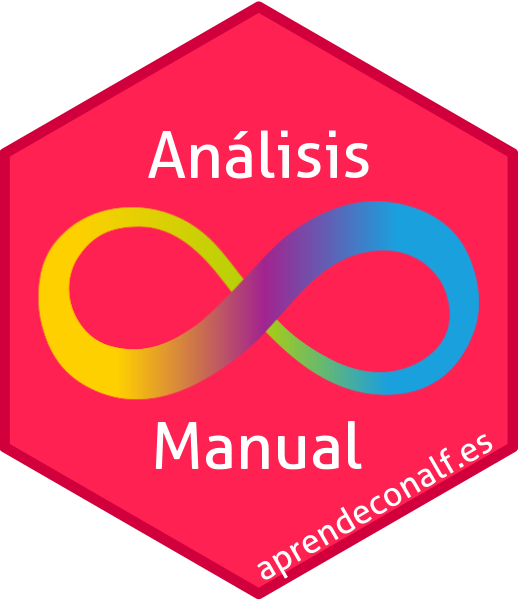
\includegraphics[width=0.4\textwidth]{img/logos/sticker.png}
\end{center}

\vfill

\begin{flushleft}
\begin{tabular}{ll}

\includegraphics[width=0.1\textwidth]{img/logos/aprendeconalf.png} & \parbox[b]{5cm}{\Large\textsf{Alfredo
Sánchez
Alberca}\\ \textsf{asalber@ceu.es} \\ \textsf{https://aprendeconalf.es}}
\end{tabular}
\end{flushleft}
\end{titlepage}
\renewcommand*\contentsname{Tabla de contenidos}
{
\setcounter{tocdepth}{2}
\tableofcontents
}

\bookmarksetup{startatroot}

\chapter*{Prefacio}\label{prefacio}
\addcontentsline{toc}{chapter}{Prefacio}

\markboth{Prefacio}{Prefacio}

¡Bienvenido al Manual de Python!

\href{https://www.python.org/}{Python} es uno de los lenguajes de
programación más extendidos, que se caracteriza por ser fácil de
aprender debido a que su sintaxis es fácil de entender para los humanos.
En este manual se presentan los conceptos básicos para iniciarse en la
programación con este lenguaje, con abundantes ejemplos.

\section*{Capítulos}\label{capuxedtulos}
\addcontentsline{toc}{section}{Capítulos}

\markright{Capítulos}

\begin{enumerate}
\def\labelenumi{\arabic{enumi}.}
\tightlist
\item
  \href{01-introduccion-python.qmd}{Introducción a Python}
\item
  \href{02-tipos-datos-simples.qmd}{Tipos de Datos Primitivos Simples}
\item
  \href{03-entrada-salida.qmd}{Entrada y Salida por Terminal}
\item
  \href{04-condicionales.qmd}{Condicionales}
\item
  \href{05-bucles.qmd}{Bucles}
\item
  \href{06-listas.qmd}{Listas}
\item
  \href{07-tuplas.qmd}{Tuplas}
\item
  \href{08-diccionarios.qmd}{Diccionarios}
\item
  \href{09-funciones.qmd}{Funciones}
\item
  \href{10-programacion-funcional.qmd}{Programación funcional}
\item
  \href{11-comprension-colecciones.qmd}{Comprensión de Colecciones}
\item
  \href{12-ficheros.qmd}{Ficheros}
\item
  \href{13-excepciones.qmd}{Excepciones}
\item
  \href{14-objetos.qmd}{Programación Orientada a Objetos}
\item
  \href{15-modulos.qmd}{Módulos}
\item
  \href{16-datetime.qmd}{La librería Datetime}
\item
  \href{17-numpy.qmd}{La librería Numpy}
\item
  \href{18-pandas.qmd}{La librería Pandas}
\item
  \href{19-matplotlib.qmd}{La librería Matplotlib}
\end{enumerate}

\section*{Apéndices}\label{apuxe9ndices}
\addcontentsline{toc}{section}{Apéndices}

\markright{Apéndices}

\begin{enumerate}
\def\labelenumi{\arabic{enumi}.}
\setcounter{enumi}{19}
\tightlist
\item
  \href{20-depuracion.qmd}{Depuración de código}
\item
  \href{21-referencias.qmd}{Referencias}
\end{enumerate}

\section*{Licencia}\label{licencia}
\addcontentsline{toc}{section}{Licencia}

\markright{Licencia}

Esta obra está bajo una licencia Reconocimiento -- No comercial --
Compartir bajo la misma licencia 3.0 España de Creative Commons. Para
ver una copia de esta licencia, visite
\url{https://creativecommons.org/licenses/by-nc-sa/3.0/es/}.

Con esta licencia eres libre de:

\begin{itemize}
\tightlist
\item
  Copiar, distribuir y mostrar este trabajo.
\item
  Realizar modificaciones de este trabajo.
\end{itemize}

Bajo las siguientes condiciones:

\begin{itemize}
\item
  \textbf{Reconocimiento}. Debe reconocer los créditos de la obra de la
  manera especificada por el autor o el licenciador (pero no de una
  manera que sugiera que tiene su apoyo o apoyan el uso que hace de su
  obra).
\item
  \textbf{No comercial}. No puede utilizar esta obra para fines
  comerciales.
\item
  \textbf{Compartir bajo la misma licencia}. Si altera o transforma esta
  obra, o genera una obra derivada, sólo puede distribuir la obra
  generada bajo una licencia idéntica a ésta.
\end{itemize}

Al reutilizar o distribuir la obra, tiene que dejar bien claro los
términos de la licencia de esta obra.

\bookmarksetup{startatroot}

\chapter{Introducción a Python}\label{introducciuxf3n-a-python}

\section{¿Qué es Python?}\label{quuxe9-es-python}

\href{https://www.python.org/}{Python} es un lenguaje de programación de
alto nivel multiparadigma que permite:

\begin{itemize}
\tightlist
\item
  Programación imperativa
\item
  Programación funcional
\item
  Programación orientada a objetos
\end{itemize}

Fue creado por Guido van Rossum en 1990 aunque actualmente es
desarrollado y mantenido por la
\href{https://www.python.org/psf-landing/}{Python Software Foundation}

\section{Principales ventajas de
Python}\label{principales-ventajas-de-python}

\begin{itemize}
\tightlist
\item
  Es de código abierto (certificado por la OSI).
\item
  Es interpretable y compilable.
\item
  Es fácil de aprender gracias a que su sintaxis es bastante legible
  para los humanos.
\item
  Es un lenguaje maduro (29 años).
\item
  Es fácilmente extensible e integrable en otros lenguajes (C, java).
\item
  Esta mantenido por una gran comunidad de desarrolladores y hay
  multitud de recursos para su aprendizaje.
\end{itemize}

\section{Tipos de ejecución}\label{tipos-de-ejecuciuxf3n}

\subsection{Interpretado en la consola de
Python}\label{interpretado-en-la-consola-de-python}

Se ejecuta cada instrucción que introduce el usuario de manera
interactiva.

\begin{Shaded}
\begin{Highlighting}[]
\OperatorTok{\textgreater{}}\NormalTok{ python}
\OperatorTok{\textgreater{}\textgreater{}\textgreater{}}\NormalTok{ name }\ExtensionTok{=} \StringTok{"Alf"}
\OperatorTok{\textgreater{}\textgreater{}\textgreater{}}\NormalTok{ print}\KeywordTok{(}\StringTok{"Hola "}\ExtensionTok{,}\NormalTok{ name}\KeywordTok{)}
\ExtensionTok{Hola}\NormalTok{ Alf}
\end{Highlighting}
\end{Shaded}

\subsection{Interpretado en fichero}\label{interpretado-en-fichero}

Se leen y se ejecutan una a una todas las instrucciones del fichero.

\begin{Shaded}
\begin{Highlighting}[]
\CommentTok{\# Fichero hola.py}
\NormalTok{name }\OperatorTok{=} \StringTok{"Alf"}
\BuiltInTok{print}\NormalTok{(}\StringTok{"Hola "}\NormalTok{, name)}
\end{Highlighting}
\end{Shaded}

\begin{Shaded}
\begin{Highlighting}[]
\OperatorTok{\textgreater{}}\NormalTok{ python }\ExtensionTok{hola.py}
\ExtensionTok{Hola}\NormalTok{ Alf}
\end{Highlighting}
\end{Shaded}

También se puede hacer el fichero ejecutable indicando en la primera
línea la ruta hasta el intérprete de Python.

\begin{Shaded}
\begin{Highlighting}[]
\CommentTok{\#!/usr/bin/python3}
\NormalTok{name }\OperatorTok{=} \StringTok{"Alf"}
\BuiltInTok{print}\NormalTok{(}\StringTok{"Hola"}\NormalTok{, name)}
\end{Highlighting}
\end{Shaded}

\begin{Shaded}
\begin{Highlighting}[]
\OperatorTok{\textgreater{}}\NormalTok{ chmod }\ExtensionTok{+x}\NormalTok{ hola.py}
\OperatorTok{\textgreater{}}\NormalTok{ ./hola.py}
\ExtensionTok{Hola}\NormalTok{ Alf}
\end{Highlighting}
\end{Shaded}

\subsection{Compilado a bytecode}\label{compilado-a-bytecode}

\begin{Shaded}
\begin{Highlighting}[]
\CommentTok{\# Fichero hola.py}
\NormalTok{name }\OperatorTok{=} \StringTok{"Alf"}
\BuiltInTok{print}\NormalTok{(}\StringTok{"Hola "} \OperatorTok{+}\NormalTok{ name)}
\end{Highlighting}
\end{Shaded}

\begin{Shaded}
\begin{Highlighting}[]
\OperatorTok{\textgreater{}}\NormalTok{ python }\ExtensionTok{{-}O} \AttributeTok{{-}m}\NormalTok{ py\_compile hola.py}
\OperatorTok{\textgreater{}}\NormalTok{ python }\ExtensionTok{\_\_pycache\_\_/hola.cpython{-}37.pyc}
\ExtensionTok{Hola}\NormalTok{ Alf}
\end{Highlighting}
\end{Shaded}

\subsection{Compilado a ejecutable del
sistema}\label{compilado-a-ejecutable-del-sistema}

Hay distintos paquetes que permiten compilar a un ejecutable del sistema
operativo usado, por ejemplo \texttt{pyinstaller}.

\begin{Shaded}
\begin{Highlighting}[]
\OperatorTok{\textgreater{}}\NormalTok{ conda }\FunctionTok{install}\NormalTok{ pyinstaller}
\OperatorTok{\textgreater{}}\NormalTok{ pyinstaller }\ExtensionTok{hola.py}
\OperatorTok{\textgreater{}}\NormalTok{ ./dist/hola/hola}
\ExtensionTok{Hola}\NormalTok{ Alf}
\end{Highlighting}
\end{Shaded}

\bookmarksetup{startatroot}

\chapter{Tipos de Datos Primitivos
Simples}\label{tipos-de-datos-primitivos-simples}

\section{Tipos de datos primitivos
simples}\label{tipos-de-datos-primitivos-simples-1}

\begin{itemize}
\tightlist
\item
  \textbf{Números} (numbers): Secuencia de dígitos (pueden incluir el -
  para negativos y el . para decimales) que representan números.\\
  \textbf{Ejemplo}. 0, -1, 3.1415.
\item
  \textbf{Cadenas} (strings): Secuencia de caracteres alfanuméricos que
  representan texto. Se escriben entre comillas simples o dobles.\\
  \textbf{Ejemplo}. `Hola', ``Adiós''.
\item
  \textbf{Booleanos} (boolean): Contiene únicamente dos elementos
  \texttt{True} y \texttt{False} que representan los valores lógicos
  verdadero y falso respectivamente.
\end{itemize}

Estos datos son inmutables, es decir, su valor es constante y no puede
cambiar.

\section{Tipos de datos primitivos compuestos
(contenedores)}\label{tipos-de-datos-primitivos-compuestos-contenedores}

\begin{itemize}
\tightlist
\item
  \textbf{Listas} (lists): Colecciones de objetos que representan
  secuencias ordenadas de objetos de distintos tipos. Se representan con
  corchetes y los elementos se separan por comas.\\
  \textbf{Ejemplo}. {[}1, ``dos'', {[}3, 4{]}, True{]}.
\item
  \textbf{Tuplas} (tuples). Colecciones de objetos que representan
  secuencias ordenadas de objetos de distintos tipos. A diferencia de
  las listas son inmutables, es decir, que no cambian durante la
  ejecución. Se representan mediante paréntesis y los elementos se
  separan por comas.\\
  \textbf{Ejemplo}. (1, `dos', 3)
\item
  \textbf{Diccionarios} (dictionaries): Colecciones de objetos con una
  clave asociada. Se representan con llaves, los pares separados por
  comas y cada par contiene una clave y un objeto asociado separados por
  dos puntos.\\
  \textbf{Ejemplo}. \{`pi':3.1416, `e':2.718\}.
\end{itemize}

\section{\texorpdfstring{Clase de un dato
(\texttt{type()})}{Clase de un dato (type())}}\label{clase-de-un-dato-type}

La clase a la que pertenece un dato se obtiene con el comando
\texttt{type()}

\begin{Shaded}
\begin{Highlighting}[]
\OperatorTok{\textgreater{}\textgreater{}\textgreater{}} \BuiltInTok{type}\NormalTok{(}\DecValTok{1}\NormalTok{)}
\OperatorTok{\textless{}}\KeywordTok{class} \StringTok{\textquotesingle{}int\textquotesingle{}}\OperatorTok{\textgreater{}}
\OperatorTok{\textgreater{}\textgreater{}\textgreater{}} \BuiltInTok{type}\NormalTok{(}\StringTok{"Hola"}\NormalTok{)}
\OperatorTok{\textless{}}\KeywordTok{class} \StringTok{\textquotesingle{}str\textquotesingle{}}\OperatorTok{\textgreater{}}
\OperatorTok{\textgreater{}\textgreater{}\textgreater{}} \BuiltInTok{type}\NormalTok{([}\DecValTok{1}\NormalTok{, }\StringTok{"dos"}\NormalTok{, [}\DecValTok{3}\NormalTok{, }\DecValTok{4}\NormalTok{], }\VariableTok{True}\NormalTok{])}
\OperatorTok{\textless{}}\KeywordTok{class} \StringTok{\textquotesingle{}list\textquotesingle{}}\OperatorTok{\textgreater{}}
\OperatorTok{\textgreater{}\textgreater{}\textgreater{}}\BuiltInTok{type}\NormalTok{(\{}\StringTok{\textquotesingle{}pi\textquotesingle{}}\NormalTok{:}\FloatTok{3.1416}\NormalTok{, }\StringTok{\textquotesingle{}e\textquotesingle{}}\NormalTok{:}\FloatTok{2.718}\NormalTok{\})}
\OperatorTok{\textless{}}\KeywordTok{class} \StringTok{\textquotesingle{}dict\textquotesingle{}}\OperatorTok{\textgreater{}}
\OperatorTok{\textgreater{}\textgreater{}\textgreater{}}\BuiltInTok{type}\NormalTok{((}\DecValTok{1}\NormalTok{, }\StringTok{\textquotesingle{}dos\textquotesingle{}}\NormalTok{, }\DecValTok{3}\NormalTok{))}
\OperatorTok{\textless{}}\KeywordTok{class} \StringTok{\textquotesingle{}tuple\textquotesingle{}}\OperatorTok{\textgreater{}}
\end{Highlighting}
\end{Shaded}

\section{\texorpdfstring{Números (clases \texttt{int} y
\texttt{float})}{Números (clases int y float)}}\label{nuxfameros-clases-int-y-float}

Secuencia de dígitos (pueden incluir el - para negativos y el . para
decimales) que representan números. Pueden ser enteros (\texttt{int}) o
reales (\texttt{float}).

\begin{Shaded}
\begin{Highlighting}[]
\OperatorTok{\textgreater{}\textgreater{}\textgreater{}} \BuiltInTok{type}\NormalTok{(}\DecValTok{1}\NormalTok{)}
\OperatorTok{\textless{}}\KeywordTok{class} \StringTok{\textquotesingle{}int\textquotesingle{}}\OperatorTok{\textgreater{}}
\OperatorTok{\textgreater{}\textgreater{}\textgreater{}} \BuiltInTok{type}\NormalTok{(}\OperatorTok{{-}}\DecValTok{2}\NormalTok{)}
\OperatorTok{\textless{}}\KeywordTok{class} \StringTok{\textquotesingle{}int\textquotesingle{}}\OperatorTok{\textgreater{}}
\OperatorTok{\textgreater{}\textgreater{}\textgreater{}} \BuiltInTok{type}\NormalTok{(}\FloatTok{2.3}\NormalTok{)}
\OperatorTok{\textless{}}\KeywordTok{class} \StringTok{\textquotesingle{}float\textquotesingle{}}\OperatorTok{\textgreater{}}
\end{Highlighting}
\end{Shaded}

\subsection{Operadores aritméticos}\label{operadores-aritmuxe9ticos}

\begin{itemize}
\tightlist
\item
  Operadores aritméticos: \texttt{+} (suma), \texttt{-} (resta),
  \texttt{*} (producto), \texttt{/} (cociente), \texttt{//} (cociente
  división entera), \texttt{\%} (resto división entera), \texttt{**}
  (potencia).
\end{itemize}

Orden de prioridad de evaluación:

{\def\LTcaptype{none} % do not increment counter
\begin{longtable}[]{@{}cc@{}}
\toprule\noalign{}
\endhead
\bottomrule\noalign{}
\endlastfoot
1 & Funciones predefinidas \\
2 & Potencias \\
3 & Productos y cocientes \\
4 & Sumas y restas \\
& \\
\end{longtable}
}

Se puede saltar el orden de evaluación utilizando paréntesis
\texttt{(\ )}.

\begin{Shaded}
\begin{Highlighting}[]
\OperatorTok{\textgreater{}\textgreater{}\textgreater{}} \DecValTok{2}\OperatorTok{+}\DecValTok{3}
\DecValTok{5}
\OperatorTok{\textgreater{}\textgreater{}\textgreater{}} \DecValTok{5}\OperatorTok{*{-}}\DecValTok{2}
\OperatorTok{{-}}\DecValTok{10}
\OperatorTok{\textgreater{}\textgreater{}\textgreater{}} \DecValTok{5}\OperatorTok{/}\DecValTok{2}
\FloatTok{2.5}
\OperatorTok{\textgreater{}\textgreater{}\textgreater{}} \DecValTok{5}\OperatorTok{//}\DecValTok{2}
\DecValTok{2}
\OperatorTok{\textgreater{}\textgreater{}\textgreater{}}\NormalTok{ (}\DecValTok{2}\OperatorTok{+}\DecValTok{3}\NormalTok{)}\OperatorTok{**}\DecValTok{2}
\DecValTok{25}
\end{Highlighting}
\end{Shaded}

\subsection{Operadores lógicos con
números}\label{operadores-luxf3gicos-con-nuxfameros}

Devuelven un valor lógico o booleano.

\begin{itemize}
\tightlist
\item
  Operadores lógicos: \texttt{==} (igual que), \texttt{\textgreater{}}
  (mayor que), \texttt{\textless{}} (menor que),
  \texttt{\textgreater{}=} (mayor o igual que), \texttt{\textless{}=}
  (menor o igual que), \texttt{!=} (distinto de).
\end{itemize}

\begin{Shaded}
\begin{Highlighting}[]
\OperatorTok{\textgreater{}\textgreater{}\textgreater{}} \DecValTok{3}\OperatorTok{==}\DecValTok{3}
\VariableTok{True}
\OperatorTok{\textgreater{}\textgreater{}\textgreater{}} \FloatTok{3.1}\OperatorTok{\textless{}=}\DecValTok{3}
\VariableTok{False}
\OperatorTok{\textgreater{}\textgreater{}\textgreater{}} \OperatorTok{{-}}\DecValTok{1}\OperatorTok{!=}\DecValTok{1}
\VariableTok{True}
\end{Highlighting}
\end{Shaded}

\section{\texorpdfstring{Cadenas (clase
\texttt{str})}{Cadenas (clase str)}}\label{cadenas-clase-str}

Secuencia de caracteres alfanuméricos que representan texto. Se escriben
entre comillas sencillas ' o dobles ``.

\begin{Shaded}
\begin{Highlighting}[]
\CommentTok{\textquotesingle{}Python\textquotesingle{}}
\CommentTok{"123"}
\CommentTok{\textquotesingle{}True\textquotesingle{}}
\CommentTok{\# Cadena vacía}
\CommentTok{\textquotesingle{}\textquotesingle{}}
\CommentTok{\# Cadena con un espacio en blanco}
\CommentTok{\textquotesingle{} \textquotesingle{}}
\CommentTok{\# Cambio de línea}
\CommentTok{\textquotesingle{}}\CharTok{\textbackslash{}n}\CommentTok{\textquotesingle{}}
\CommentTok{\# Tabulador}
\CommentTok{\textquotesingle{}}\CharTok{\textbackslash{}t}\CommentTok{\textquotesingle{}}
\end{Highlighting}
\end{Shaded}

\subsection{Acceso a los elementos de una
cadena}\label{acceso-a-los-elementos-de-una-cadena}

Cada carácter tiene asociado un índice que permite acceder a él.

{\def\LTcaptype{none} % do not increment counter
\begin{longtable}[]{@{}ccccccc@{}}
\toprule\noalign{}
Cadena & \texttt{P} & \texttt{y} & \texttt{t} & \texttt{h} & \texttt{o}
& \texttt{n} \\
\midrule\noalign{}
\endhead
\bottomrule\noalign{}
\endlastfoot
Índice positivo & 0 & 1 & 2 & 3 & 4 & 5 \\
Índice negativo & -6 & -5 & -4 & -3 & -2 & -1 \\
\end{longtable}
}

\begin{itemize}
\tightlist
\item
  \texttt{c{[}i{]}} devuelve el carácter de la cadena \texttt{c} con el
  índice \texttt{i}.
\end{itemize}

\begin{tcolorbox}[enhanced jigsaw, arc=.35mm, bottomrule=.15mm, bottomtitle=1mm, breakable, colback=white, colbacktitle=quarto-callout-warning-color!10!white, colframe=quarto-callout-warning-color-frame, coltitle=black, left=2mm, leftrule=.75mm, opacityback=0, opacitybacktitle=0.6, rightrule=.15mm, title=\textcolor{quarto-callout-warning-color}{\faExclamationTriangle}\hspace{0.5em}{Advertencia}, titlerule=0mm, toprule=.15mm, toptitle=1mm]

El índice del primer carácter de la cadena es 0.

\end{tcolorbox}

También se pueden utilizar índices negativos para recorrer la cadena del
final al principio.

\begin{tcolorbox}[enhanced jigsaw, arc=.35mm, bottomrule=.15mm, bottomtitle=1mm, breakable, colback=white, colbacktitle=quarto-callout-warning-color!10!white, colframe=quarto-callout-warning-color-frame, coltitle=black, left=2mm, leftrule=.75mm, opacityback=0, opacitybacktitle=0.6, rightrule=.15mm, title=\textcolor{quarto-callout-warning-color}{\faExclamationTriangle}\hspace{0.5em}{Advertencia}, titlerule=0mm, toprule=.15mm, toptitle=1mm]

El índice del último carácter de la cadena es -1.

\end{tcolorbox}

\begin{Shaded}
\begin{Highlighting}[]
\OperatorTok{\textgreater{}\textgreater{}\textgreater{}} \StringTok{\textquotesingle{}Python\textquotesingle{}}\NormalTok{[}\DecValTok{0}\NormalTok{]}
\CommentTok{\textquotesingle{}P\textquotesingle{}}
\OperatorTok{\textgreater{}\textgreater{}\textgreater{}} \StringTok{\textquotesingle{}Python\textquotesingle{}}\NormalTok{[}\DecValTok{1}\NormalTok{]}
\CommentTok{\textquotesingle{}y\textquotesingle{}}
\OperatorTok{\textgreater{}\textgreater{}\textgreater{}} \StringTok{\textquotesingle{}Python\textquotesingle{}}\NormalTok{[}\OperatorTok{{-}}\DecValTok{1}\NormalTok{]}
\CommentTok{\textquotesingle{}n\textquotesingle{}}
\OperatorTok{\textgreater{}\textgreater{}\textgreater{}} \StringTok{\textquotesingle{}Python\textquotesingle{}}\NormalTok{[}\DecValTok{6}\NormalTok{]}
\NormalTok{Traceback (most recent call last):}
\NormalTok{  File }\StringTok{"\textless{}stdin\textgreater{}"}\NormalTok{, line }\DecValTok{1}\NormalTok{, }\KeywordTok{in} \OperatorTok{\textless{}}\NormalTok{module}\OperatorTok{\textgreater{}}
\PreprocessorTok{IndexError}\NormalTok{: string index out of }\BuiltInTok{range}
\end{Highlighting}
\end{Shaded}

\subsection{Subcadenas}\label{subcadenas}

\begin{itemize}
\tightlist
\item
  \texttt{c{[}i:j:k{]}} : Devuelve la subcadena de \texttt{c} desde el
  carácter con el índice \texttt{i} hasta el carácter anterior al índice
  \texttt{j}, tomando caracteres cada \texttt{k}.
\end{itemize}

\begin{Shaded}
\begin{Highlighting}[]
\OperatorTok{\textgreater{}\textgreater{}\textgreater{}} \StringTok{\textquotesingle{}Python\textquotesingle{}}\NormalTok{[}\DecValTok{1}\NormalTok{:}\DecValTok{4}\NormalTok{]}
\CommentTok{\textquotesingle{}yth\textquotesingle{}}
\OperatorTok{\textgreater{}\textgreater{}\textgreater{}} \StringTok{\textquotesingle{}Python\textquotesingle{}}\NormalTok{[}\DecValTok{1}\NormalTok{:}\DecValTok{1}\NormalTok{]}
\CommentTok{\textquotesingle{}\textquotesingle{}}
\OperatorTok{\textgreater{}\textgreater{}\textgreater{}} \StringTok{\textquotesingle{}Python\textquotesingle{}}\NormalTok{[}\DecValTok{2}\NormalTok{:]}
\CommentTok{\textquotesingle{}thon\textquotesingle{}}
\OperatorTok{\textgreater{}\textgreater{}\textgreater{}} \StringTok{\textquotesingle{}Python\textquotesingle{}}\NormalTok{[:}\OperatorTok{{-}}\DecValTok{2}\NormalTok{]}
\CommentTok{\textquotesingle{}Pyth\textquotesingle{}}
\OperatorTok{\textgreater{}\textgreater{}\textgreater{}} \StringTok{\textquotesingle{}Python\textquotesingle{}}\NormalTok{[:]}
\CommentTok{\textquotesingle{}Python\textquotesingle{}}
\OperatorTok{\textgreater{}\textgreater{}\textgreater{}} \StringTok{\textquotesingle{}Python\textquotesingle{}}\NormalTok{[}\DecValTok{0}\NormalTok{:}\DecValTok{6}\NormalTok{:}\DecValTok{2}\NormalTok{]}
\CommentTok{\textquotesingle{}Pto\textquotesingle{}}
\end{Highlighting}
\end{Shaded}

\subsection{Operaciones con cadenas}\label{operaciones-con-cadenas}

\begin{itemize}
\tightlist
\item
  \texttt{c1\ +\ c2} : Devuelve la cadena resultado de concatenar las
  cadenas \texttt{c1} y \texttt{c2}.
\item
  \texttt{c\ *\ n} : Devuelve la cadena resultado de concatenar
  \texttt{n} copias de la cadena \texttt{c}.
\item
  \texttt{c1\ in\ c2} : Devuelve \texttt{True} si \texttt{c1} es una
  cadena concenida en \texttt{c2} y \texttt{False} en caso contrario.
\item
  \texttt{c1\ not\ in\ c2} : Devuelve \texttt{True} si \texttt{c1} es
  una cadena no concenida en \texttt{c2} y \texttt{False} en caso
  contrario.
\end{itemize}

\begin{Shaded}
\begin{Highlighting}[]
\OperatorTok{\textgreater{}\textgreater{}\textgreater{}} \StringTok{\textquotesingle{}Me gusta \textquotesingle{}} \OperatorTok{+} \StringTok{\textquotesingle{}Python\textquotesingle{}}
\CommentTok{\textquotesingle{}Me gusta Python\textquotesingle{}}
\OperatorTok{\textgreater{}\textgreater{}\textgreater{}} \StringTok{\textquotesingle{}Python\textquotesingle{}} \OperatorTok{*} \DecValTok{3}
\CommentTok{\textquotesingle{}PythonPythonPython\textquotesingle{}}
\OperatorTok{\textgreater{}\textgreater{}\textgreater{}} \StringTok{\textquotesingle{}y\textquotesingle{}} \KeywordTok{in} \StringTok{\textquotesingle{}Python\textquotesingle{}}
\VariableTok{True}
\OperatorTok{\textgreater{}\textgreater{}\textgreater{}} \StringTok{\textquotesingle{}tho\textquotesingle{}} \KeywordTok{in} \StringTok{\textquotesingle{}Python\textquotesingle{}}
\VariableTok{True}
\OperatorTok{\textgreater{}\textgreater{}\textgreater{}} \StringTok{\textquotesingle{}to\textquotesingle{}} \KeywordTok{not} \KeywordTok{in} \StringTok{\textquotesingle{}Python\textquotesingle{}}
\VariableTok{True}
\end{Highlighting}
\end{Shaded}

\subsection{Operaciones de comparación de
cadenas}\label{operaciones-de-comparaciuxf3n-de-cadenas}

\begin{itemize}
\tightlist
\item
  \texttt{c1\ ==\ c2} : Devuelve \texttt{True} si la cadena \texttt{c1}
  es igual que la cadena \texttt{c2} y \texttt{False} en caso contrario.
\item
  \texttt{c1\ \textgreater{}\ c2} : Devuelve \texttt{True} si la cadena
  \texttt{c1} sucede a la cadena \texttt{c2} y \texttt{False} en caso
  contrario.
\item
  \texttt{c1\ \textless{}\ c2} : Devuelve \texttt{True} si la cadena
  \texttt{c1} antecede a la cadena \texttt{c2} y \texttt{False} en caso
  contrario.
\item
  \texttt{c1\ \textgreater{}=\ c2} : Devuelve \texttt{True} si la cadena
  \texttt{c1} sucede o es igual a la cadena \texttt{c2} y \texttt{False}
  en caso contrario.
\item
  \texttt{c1\ \textless{}=\ c2} : Devuelve \texttt{True} si la cadena
  \texttt{c1} antecede o es igual a la cadena \texttt{c2} y
  \texttt{False} en caso contrario.
\item
  \texttt{c1\ !=\ c2} : Devuelve \texttt{True} si la cadena \texttt{c1}
  es distinta de la cadena \texttt{c2} y \texttt{False} en caso
  contrario.
\end{itemize}

\begin{tcolorbox}[enhanced jigsaw, arc=.35mm, bottomrule=.15mm, bottomtitle=1mm, breakable, colback=white, colbacktitle=quarto-callout-warning-color!10!white, colframe=quarto-callout-warning-color-frame, coltitle=black, left=2mm, leftrule=.75mm, opacityback=0, opacitybacktitle=0.6, rightrule=.15mm, title=\textcolor{quarto-callout-warning-color}{\faExclamationTriangle}\hspace{0.5em}{Advertencia}, titlerule=0mm, toprule=.15mm, toptitle=1mm]

Utilizan el orden establecido en el
\href{https://www.codigosascii.com/}{código ASCII}.

\end{tcolorbox}

\begin{Shaded}
\begin{Highlighting}[]
\OperatorTok{\textgreater{}\textgreater{}\textgreater{}} \StringTok{\textquotesingle{}Python\textquotesingle{}} \OperatorTok{==} \StringTok{\textquotesingle{}python\textquotesingle{}}
\VariableTok{False}
\OperatorTok{\textgreater{}\textgreater{}\textgreater{}} \StringTok{\textquotesingle{}Python\textquotesingle{}} \OperatorTok{\textless{}} \StringTok{\textquotesingle{}python\textquotesingle{}}
\VariableTok{True}
\OperatorTok{\textgreater{}\textgreater{}\textgreater{}} \StringTok{\textquotesingle{}a\textquotesingle{}} \OperatorTok{\textgreater{}} \StringTok{\textquotesingle{}Z\textquotesingle{}}
\VariableTok{True}
\OperatorTok{\textgreater{}\textgreater{}\textgreater{}} \StringTok{\textquotesingle{}A\textquotesingle{}} \OperatorTok{\textgreater{}=} \StringTok{\textquotesingle{}Z\textquotesingle{}}
\VariableTok{False}
\OperatorTok{\textgreater{}\textgreater{}\textgreater{}} \StringTok{\textquotesingle{}\textquotesingle{}} \OperatorTok{\textless{}} \StringTok{\textquotesingle{}Python\textquotesingle{}}
\VariableTok{True}
\end{Highlighting}
\end{Shaded}

\subsection{Funciones de cadenas}\label{funciones-de-cadenas}

\begin{itemize}
\tightlist
\item
  \texttt{len(c)} : Devuelve el número de caracteres de la cadena
  \texttt{c}.
\item
  \texttt{min(c)} : Devuelve el carácter menor de la cadena \texttt{c}.
\item
  \texttt{max(c)} : Devuelve el carácter mayor de la cadena \texttt{c}.
\item
  \texttt{c.upper()} : Devuelve la cadena con los mismos caracteres que
  la cadena \texttt{c} pero en mayúsculas.
\item
  \texttt{c.lower()} : Devuelve la cadena con los mismos caracteres que
  la cadena \texttt{c} pero en minúsculas.
\item
  \texttt{c.title()} : Devuelve la cadena con los mismos caracteres que
  la cadena \texttt{c} con el primer carácter en mayúsculas y el resto
  en minúsculas.
\item
  \texttt{c.split(delimitador)} : Devuelve la lista formada por las
  subcadenas que resultan de partir la cadena \texttt{c} usando como
  delimitador la cadena \texttt{delimitador}. Si no se especifica el
  delimitador utiliza por defecto el espacio en blanco.
\end{itemize}

\begin{Shaded}
\begin{Highlighting}[]
\OperatorTok{\textgreater{}\textgreater{}\textgreater{}} \BuiltInTok{len}\NormalTok{(}\StringTok{\textquotesingle{}Python\textquotesingle{}}\NormalTok{)}
\DecValTok{6}
\OperatorTok{\textgreater{}\textgreater{}\textgreater{}} \BuiltInTok{min}\NormalTok{(}\StringTok{\textquotesingle{}Python\textquotesingle{}}\NormalTok{)}
\CommentTok{\textquotesingle{}P\textquotesingle{}}
\OperatorTok{\textgreater{}\textgreater{}\textgreater{}} \BuiltInTok{max}\NormalTok{(}\StringTok{\textquotesingle{}Python\textquotesingle{}}\NormalTok{)}
\CommentTok{\textquotesingle{}y\textquotesingle{}}
\OperatorTok{\textgreater{}\textgreater{}\textgreater{}} \StringTok{\textquotesingle{}Python\textquotesingle{}}\NormalTok{.upper()}
\CommentTok{\textquotesingle{}PYTHON\textquotesingle{}}
\OperatorTok{\textgreater{}\textgreater{}\textgreater{}} \StringTok{\textquotesingle{}A,B,C\textquotesingle{}}\NormalTok{.split(}\StringTok{\textquotesingle{},\textquotesingle{}}\NormalTok{)}
\NormalTok{[}\StringTok{\textquotesingle{}A\textquotesingle{}}\NormalTok{, }\StringTok{\textquotesingle{}B\textquotesingle{}}\NormalTok{, }\StringTok{\textquotesingle{}C\textquotesingle{}}\NormalTok{]}
\OperatorTok{\textgreater{}\textgreater{}\textgreater{}} \StringTok{\textquotesingle{}I love Python\textquotesingle{}}\NormalTok{.split()}
\NormalTok{[}\StringTok{\textquotesingle{}I\textquotesingle{}}\NormalTok{, }\StringTok{\textquotesingle{}love\textquotesingle{}}\NormalTok{, }\StringTok{\textquotesingle{}Python\textquotesingle{}}\NormalTok{]}
\end{Highlighting}
\end{Shaded}

\subsection{\texorpdfstring{Cadenas formateadas
(\texttt{format()})}{Cadenas formateadas (format())}}\label{cadenas-formateadas-format}

\begin{itemize}
\tightlist
\item
  \texttt{c.format(valores)}: Devuelve la cadena \texttt{c} tras
  sustituir los valores de la secuencia \texttt{valores} en los
  marcadores de posición de \texttt{c}. Los marcadores de posición se
  indican mediante llaves \texttt{\{\}} en la cadena \texttt{c}, y el
  reemplazo de los valores se puede realizar por posición, indicando en
  número de orden del valor dentro de las llaves, o por nombre,
  indicando el nombre del valor, siempre y cuando los valores se pasen
  con el formato \texttt{nombre\ =\ valor}.
\end{itemize}

\begin{Shaded}
\begin{Highlighting}[]
\OperatorTok{\textgreater{}\textgreater{}\textgreater{}} \StringTok{\textquotesingle{}Un }\SpecialCharTok{\{\}}\StringTok{ vale }\SpecialCharTok{\{\}}\StringTok{ }\SpecialCharTok{\{\}}\StringTok{\textquotesingle{}}\NormalTok{.}\BuiltInTok{format}\NormalTok{(}\StringTok{\textquotesingle{}€\textquotesingle{}}\NormalTok{, }\FloatTok{1.12}\NormalTok{, }\StringTok{\textquotesingle{}$\textquotesingle{}}\NormalTok{)}
\CommentTok{\textquotesingle{}Un € vale 1.12 $\textquotesingle{}}
\OperatorTok{\textgreater{}\textgreater{}\textgreater{}} \StringTok{\textquotesingle{}Un }\SpecialCharTok{\{2\}}\StringTok{ vale }\SpecialCharTok{\{1\}}\StringTok{ }\SpecialCharTok{\{0\}}\StringTok{\textquotesingle{}}\NormalTok{.}\BuiltInTok{format}\NormalTok{(}\StringTok{\textquotesingle{}€\textquotesingle{}}\NormalTok{, }\FloatTok{1.12}\NormalTok{, }\StringTok{\textquotesingle{}$\textquotesingle{}}\NormalTok{)}
\CommentTok{\textquotesingle{}Un $ vale 1.12 €\textquotesingle{}}
\OperatorTok{\textgreater{}\textgreater{}\textgreater{}} \StringTok{\textquotesingle{}Un }\SpecialCharTok{\{moneda1\}}\StringTok{ vale }\SpecialCharTok{\{cambio\}}\StringTok{ }\SpecialCharTok{\{moneda2\}}\StringTok{\textquotesingle{}}\NormalTok{.}\BuiltInTok{format}\NormalTok{(moneda1 }\OperatorTok{=} \StringTok{\textquotesingle{}€\textquotesingle{}}\NormalTok{, cambio }\OperatorTok{=} \FloatTok{1.12}\NormalTok{, moneda2 }\OperatorTok{=} \StringTok{\textquotesingle{}$\textquotesingle{}}\NormalTok{)}
\CommentTok{\textquotesingle{}Un € vale 1.12 $\textquotesingle{}}
\end{Highlighting}
\end{Shaded}

Los marcadores de posición, a parte de indicar la posición de los
valores de reemplazo, pueden indicar también el formato de estos. Para
ello se utiliza la siguiente sintaxis:

\begin{itemize}
\tightlist
\item
  \texttt{\{:n\}} : Alinea el valor a la izquierda rellenando con
  espacios por la derecha hasta los \texttt{n} caracteres.
\item
  \texttt{\{:\textgreater{}n\}} : Alinea el valor a la derecha
  rellenando con espacios por la izquierda hasta los \texttt{n}
  caracteres.
\item
  \texttt{\{:\^{}n\}} : Alinea el valor en el centro rellenando con
  espacios por la izquierda y por la derecha hasta los \texttt{n}
  caracteres.
\item
  \texttt{\{:nd\}} : Formatea el valor como un número entero con
  \texttt{n} caracteres rellenando con espacios blancos por la
  izquierda.
\item
  \texttt{\{:n.mf\}} : Formatea el valor como un número real con un
  tamaño de \texttt{n} caracteres (incluído el separador de decimales) y
  \texttt{m} cifras decimales, rellenando con espacios blancos por la
  izquierda.
\end{itemize}

\begin{Shaded}
\begin{Highlighting}[]
\OperatorTok{\textgreater{}\textgreater{}\textgreater{}} \StringTok{\textquotesingle{}Hoy es }\SpecialCharTok{\{:\^{}10\}}\StringTok{, mañana }\SpecialCharTok{\{:10\}}\StringTok{ y pasado }\SpecialCharTok{\{:\textgreater{}10\}}\StringTok{\textquotesingle{}}\NormalTok{.}\BuiltInTok{format}\NormalTok{(}\StringTok{\textquotesingle{}lunes\textquotesingle{}}\NormalTok{, }\StringTok{\textquotesingle{}martes\textquotesingle{}}\NormalTok{, }\StringTok{\textquotesingle{}miércoles\textquotesingle{}}\NormalTok{)}
\CommentTok{\textquotesingle{}Hoy es   lunes   , mañana martes     y pasado  miércoles\textquotesingle{}}
\OperatorTok{\textgreater{}\textgreater{}\textgreater{}} \StringTok{\textquotesingle{}Cantidad }\SpecialCharTok{\{:5d\}}\StringTok{\textquotesingle{}}\NormalTok{.}\BuiltInTok{format}\NormalTok{(}\DecValTok{12}\NormalTok{)}\StringTok{\textquotesingle{}}
\ErrorTok{\textquotesingle{}Cantidad    12\textquotesingle{}}
\ErrorTok{\textgreater{}\textgreater{}\textgreater{} \textquotesingle{}Pi vale \{:8.4f\}\textquotesingle{}.format(3.141592)}
\CommentTok{\textquotesingle{}Pi vale   3.1416\textquotesingle{}}
\end{Highlighting}
\end{Shaded}

\section{\texorpdfstring{Datos lógicos o booleanos (clase
\texttt{bool})}{Datos lógicos o booleanos (clase bool)}}\label{datos-luxf3gicos-o-booleanos-clase-bool}

Contiene únicamente dos elementos \texttt{True} y \texttt{False} que
representan los valores lógicos verdadero y falso respectivamente.

\texttt{False} tiene asociado el valor 0 y \texttt{True} tiene asociado
el valor 1.

\subsection{Operaciones con valores
lógicos}\label{operaciones-con-valores-luxf3gicos}

\begin{itemize}
\tightlist
\item
  Operadores lógicos: \texttt{==} (igual que), \texttt{\textgreater{}}
  (mayor), \texttt{\textless{}} (menor), \texttt{\textgreater{}=} (mayor
  o igual que), \texttt{\textless{}=} (menor o igual que), \texttt{!=}
  (distinto de).
\item
  \texttt{not\ b} (negación) : Devuelve \texttt{True} si el dato
  booleano \texttt{b} es \texttt{False} , y \texttt{False} en caso
  contrario.
\item
  \texttt{b1\ and\ b2} : Devuelve \texttt{True} si los datos booleanos
  \texttt{b1} y \texttt{b2} son \texttt{True}, y \texttt{False} en caso
  contrario.
\item
  \texttt{b1\ or\ b2} : Devuelve \texttt{True} si alguno de los datos
  booleanos \texttt{b1} o \texttt{b2} son \texttt{True}, y
  \texttt{False} en caso contrario.
\end{itemize}

\subsection{Tabla de verdad}\label{tabla-de-verdad}

{\def\LTcaptype{none} % do not increment counter
\begin{longtable}[]{@{}ccccc@{}}
\toprule\noalign{}
\texttt{x} & \texttt{y} & \texttt{not\ x} & \texttt{x\ and\ y} &
\texttt{x\ or\ y} \\
\midrule\noalign{}
\endhead
\bottomrule\noalign{}
\endlastfoot
\texttt{False} & \texttt{False} & \texttt{True} & \texttt{False} &
\texttt{False} \\
\texttt{False} & \texttt{True} & \texttt{True} & \texttt{False} &
\texttt{True} \\
\texttt{True} & \texttt{False} & \texttt{False} & \texttt{False} &
\texttt{True} \\
\texttt{True} & \texttt{True} & \texttt{False} & \texttt{True} &
\texttt{True} \\
\end{longtable}
}

\begin{Shaded}
\begin{Highlighting}[]
\OperatorTok{\textgreater{}\textgreater{}\textgreater{}} \KeywordTok{not} \VariableTok{True}
\VariableTok{False}
\OperatorTok{\textgreater{}\textgreater{}\textgreater{}} \VariableTok{False} \KeywordTok{or} \VariableTok{True}
\VariableTok{True}
\OperatorTok{\textgreater{}\textgreater{}\textgreater{}} \VariableTok{True} \KeywordTok{and} \VariableTok{False}
\VariableTok{False}
\OperatorTok{\textgreater{}\textgreater{}\textgreater{}} \VariableTok{True} \KeywordTok{and} \VariableTok{True}
\VariableTok{True}
\end{Highlighting}
\end{Shaded}

\section{Conversión de datos primitivos
simples}\label{conversiuxf3n-de-datos-primitivos-simples}

Las siguientes funciones convierten un dato de un tipo en otro, siempre
y cuando la conversión sea posible.

\begin{itemize}
\tightlist
\item
  \texttt{int()} convierte a entero.\\
  \textbf{Ejemplo}. \texttt{int(\textquotesingle{}12\textquotesingle{})}
  \texttt{12}\\
  \texttt{int(True)} \texttt{1}\strut \\
  \texttt{int(\textquotesingle{}c\textquotesingle{})} Error
\item
  \texttt{float()} convierte a real.\\
  \textbf{Ejemplo}.
  \texttt{float(\textquotesingle{}3.14\textquotesingle{})}
  \texttt{3.14}\\
  \texttt{float(True)} \texttt{1.0}\strut \\
  \texttt{float(\textquotesingle{}III\textquotesingle{})} Error
\item
  \texttt{str()} convierte a cadena.\\
  \textbf{Ejemplo}. \texttt{str(3.14)}
  \texttt{\textquotesingle{}3.14\textquotesingle{}}\\
  \texttt{str(True)}
  \texttt{\textquotesingle{}True\textquotesingle{}}\strut \\
\item
  \texttt{bool()} convierte a lógico.\\
  \textbf{Ejemplo}. \texttt{bool(\textquotesingle{}0\textquotesingle{})}
  \texttt{False}\\
  \texttt{bool(\textquotesingle{}3.14\textquotesingle{})}
  \texttt{True}\strut \\
  \texttt{bool(\textquotesingle{}\textquotesingle{})}
  \texttt{False}\strut \\
  \texttt{bool(\textquotesingle{}Hola\textquotesingle{})} \texttt{True}
\end{itemize}

\section{Variables}\label{variables}

Una variable es un identificador ligado a algún valor.

Reglas para nombrarlas:

\begin{itemize}
\tightlist
\item
  Comienzan siempre por una letra, seguida de otras letras o números.
\item
  No se pueden utilizarse palabras reservadas del lenguaje.
\end{itemize}

A diferencia de otros lenguajes no tienen asociado un tipo y no es
necesario declararlas antes de usarlas (tipado dinámico).

Para asignar un valor a una variable se utiliza el operador \texttt{=} y
para borrar una variable se utiliza la instrucción \texttt{del}.

\begin{Shaded}
\begin{Highlighting}[]
\NormalTok{lenguaje }\OperatorTok{=} \StringTok{\textquotesingle{}Python\textquotesingle{}}
\NormalTok{x }\OperatorTok{=} \FloatTok{3.14}
\NormalTok{y }\OperatorTok{=} \DecValTok{3} \OperatorTok{+} \DecValTok{2}
\CommentTok{\# Asignación múltiple}
\NormalTok{a1, a2 }\OperatorTok{=} \DecValTok{1}\NormalTok{, }\DecValTok{2}
\CommentTok{\# Intercambio de valores}
\NormalTok{a, b }\OperatorTok{=}\NormalTok{ b, a}
\CommentTok{\# Incremento (equivale a x = x + 2)}
\NormalTok{x }\OperatorTok{+=} \DecValTok{2}
\CommentTok{\# Decremento (equivale a x = x {-} 1)}
\NormalTok{x }\OperatorTok{{-}=} \DecValTok{1}
\CommentTok{\# Valor no definido}
\NormalTok{x }\OperatorTok{=} \VariableTok{None}
\KeywordTok{del}\NormalTok{ x}
\end{Highlighting}
\end{Shaded}

\bookmarksetup{startatroot}

\chapter{Entrada y Salida por
Terminal}\label{entrada-y-salida-por-terminal}

\section{\texorpdfstring{Entrada por terminal
(\texttt{input()})}{Entrada por terminal (input())}}\label{entrada-por-terminal-input}

Para asignar a una variable un valor introducido por el usuario en la
consola se utiliza la instrucción

\texttt{input(mensaje)} : Muestra la cadena \texttt{mensaje} por la
terminal y devuelve una cadena con la entrada del usuario.

\begin{tcolorbox}[enhanced jigsaw, arc=.35mm, bottomrule=.15mm, bottomtitle=1mm, breakable, colback=white, colbacktitle=quarto-callout-warning-color!10!white, colframe=quarto-callout-warning-color-frame, coltitle=black, left=2mm, leftrule=.75mm, opacityback=0, opacitybacktitle=0.6, rightrule=.15mm, title=\textcolor{quarto-callout-warning-color}{\faExclamationTriangle}\hspace{0.5em}{Advertencia}, titlerule=0mm, toprule=.15mm, toptitle=1mm]

El valor devuelto siempre es una cadena, incluso si el usuario introduce
un dato numérico.

\end{tcolorbox}

\begin{Shaded}
\begin{Highlighting}[]
\OperatorTok{\textgreater{}\textgreater{}\textgreater{}}\NormalTok{ language }\OperatorTok{=} \BuiltInTok{input}\NormalTok{(}\StringTok{\textquotesingle{}¿Cuál es tu lenguaje favorito? \textquotesingle{}}\NormalTok{)}
\NormalTok{¿Cuál es tu lenguaje favorito? Python}
\OperatorTok{\textgreater{}\textgreater{}\textgreater{}}\NormalTok{ language}
\CommentTok{\textquotesingle{}Python\textquotesingle{}}
\OperatorTok{\textgreater{}\textgreater{}\textgreater{}}\NormalTok{ age }\OperatorTok{=} \BuiltInTok{input}\NormalTok{(}\StringTok{\textquotesingle{}¿Cuál es tu edad? \textquotesingle{}}\NormalTok{)}
\NormalTok{¿Cuál es tu edad? }\DecValTok{20}
\OperatorTok{\textgreater{}\textgreater{}\textgreater{}}\NormalTok{ age}
\CommentTok{\textquotesingle{}20\textquotesingle{}}
\end{Highlighting}
\end{Shaded}

\section{\texorpdfstring{Salida por terminal
(\texttt{print()})}{Salida por terminal (print())}}\label{salida-por-terminal-print}

Para mostrar un dato por la terminal se utiliza la instrucción

\texttt{print(dato1,\ ...,\ sep=\textquotesingle{}\ \textquotesingle{},\ end=\textquotesingle{}\textbackslash{}n\textquotesingle{},\ file=sys.stdout})

donde

\begin{itemize}
\tightlist
\item
  \texttt{dato1,\ ...} son los datos a imprimir y pueden indicarse
  tantos como se quieran separados por comas.
\item
  \texttt{sep} establece el separador entre los datos, que por defecto
  es un espacio en blanco
  \texttt{\textquotesingle{}\ \textquotesingle{}}.
\item
  \texttt{end} indica la cadena final de la impresión, que por defecto
  es un cambio de línea \texttt{\textbackslash{}n}.
\item
  \texttt{file} indica la dirección del flujo de salida, que por defecto
  es la salida estándar \texttt{sys.stdout}.
\end{itemize}

\begin{Shaded}
\begin{Highlighting}[]
\OperatorTok{\textgreater{}\textgreater{}\textgreater{}} \BuiltInTok{print}\NormalTok{(}\StringTok{\textquotesingle{}Hola\textquotesingle{}}\NormalTok{)}
\NormalTok{Hola}
\OperatorTok{\textgreater{}\textgreater{}\textgreater{}}\NormalTok{ name }\OperatorTok{=} \StringTok{\textquotesingle{}Alf\textquotesingle{}}
\OperatorTok{\textgreater{}\textgreater{}\textgreater{}} \BuiltInTok{print}\NormalTok{(}\StringTok{\textquotesingle{}Hola\textquotesingle{}}\NormalTok{, name)}
\NormalTok{Hola Alf}
\OperatorTok{\textgreater{}\textgreater{}\textgreater{}} \BuiltInTok{print}\NormalTok{(}\StringTok{\textquotesingle{}El valor de pi es\textquotesingle{}}\NormalTok{, }\FloatTok{3.1415}\NormalTok{)}
\NormalTok{El valor de pi es }\FloatTok{3.1415}
\OperatorTok{\textgreater{}\textgreater{}\textgreater{}} \BuiltInTok{print}\NormalTok{(}\StringTok{\textquotesingle{}Hola\textquotesingle{}}\NormalTok{, name, sep}\OperatorTok{=}\StringTok{\textquotesingle{}\textquotesingle{}}\NormalTok{)}
\NormalTok{HolaAlf}
\OperatorTok{\textgreater{}\textgreater{}\textgreater{}} \BuiltInTok{print}\NormalTok{(}\StringTok{\textquotesingle{}Hola\textquotesingle{}}\NormalTok{, name, end}\OperatorTok{=}\StringTok{\textquotesingle{}!}\CharTok{\textbackslash{}n}\StringTok{\textquotesingle{}}\NormalTok{)}
\NormalTok{Hola Alf}\OperatorTok{!}
\end{Highlighting}
\end{Shaded}

\section{Salida formateada por terminal (cadenas
f)}\label{salida-formateada-por-terminal-cadenas-f}

Para construir cadenas que combinen texto con el valor de variables o
expresiones de una forma más cómoda y legible que con \texttt{format()},
Python ofrece las \textbf{cadenas f} (\emph{f-strings}). Se escriben
anteponiendo la letra \texttt{f} a la cadena, y dentro de ella se pueden
incluir variables o expresiones entre llaves \texttt{\{\}}, que serán
sustituidas por su valor.

\begin{Shaded}
\begin{Highlighting}[]
\OperatorTok{\textgreater{}\textgreater{}\textgreater{}}\NormalTok{ name }\OperatorTok{=} \StringTok{\textquotesingle{}Alf\textquotesingle{}}
\OperatorTok{\textgreater{}\textgreater{}\textgreater{}}\NormalTok{ age }\OperatorTok{=} \DecValTok{20}
\OperatorTok{\textgreater{}\textgreater{}\textgreater{}} \BuiltInTok{print}\NormalTok{(}\SpecialStringTok{f\textquotesingle{}Me llamo }\SpecialCharTok{\{}\NormalTok{name}\SpecialCharTok{\}}\SpecialStringTok{ y tengo }\SpecialCharTok{\{}\NormalTok{age}\SpecialCharTok{\}}\SpecialStringTok{ años\textquotesingle{}}\NormalTok{)}
\NormalTok{Me llamo Alf y tengo }\DecValTok{20}\NormalTok{ años}
\OperatorTok{\textgreater{}\textgreater{}\textgreater{}} \BuiltInTok{print}\NormalTok{(}\SpecialStringTok{f\textquotesingle{}El año que viene tendré }\SpecialCharTok{\{}\NormalTok{age }\OperatorTok{+} \DecValTok{1}\SpecialCharTok{\}}\SpecialStringTok{ años\textquotesingle{}}\NormalTok{)}
\NormalTok{El año que viene tendré }\DecValTok{21}\NormalTok{ años}
\end{Highlighting}
\end{Shaded}

Al igual que con \texttt{format()}, dentro de las llaves se puede
añadir, tras el signo \texttt{:}, un formato para controlar la
alineación, la anchura o el número de decimales con los que se muestra
el valor:

\begin{itemize}
\tightlist
\item
  \texttt{\{valor:n\}} : Alinea \texttt{valor} a la izquierda rellenando
  con espacios por la derecha hasta los \texttt{n} caracteres.
\item
  \texttt{\{valor:\textgreater{}n\}} : Alinea \texttt{valor} a la
  derecha rellenando con espacios por la izquierda hasta los \texttt{n}
  caracteres.
\item
  \texttt{\{valor:\^{}n\}} : Alinea \texttt{valor} en el centro
  rellenando con espacios por la izquierda y por la derecha hasta los
  \texttt{n} caracteres.
\item
  \texttt{\{valor:nd\}} : Formatea \texttt{valor} como un número entero
  con \texttt{n} caracteres rellenando con espacios en blanco por la
  izquierda.
\item
  \texttt{\{valor:n.mf\}} : Formatea \texttt{valor} como un número real
  con un tamaño de \texttt{n} caracteres (incluido el separador de
  decimales) y \texttt{m} cifras decimales, rellenando con espacios en
  blanco por la izquierda.
\end{itemize}

\begin{Shaded}
\begin{Highlighting}[]
\OperatorTok{\textgreater{}\textgreater{}\textgreater{}}\NormalTok{ pi }\OperatorTok{=} \FloatTok{3.141592}
\OperatorTok{\textgreater{}\textgreater{}\textgreater{}} \BuiltInTok{print}\NormalTok{(}\SpecialStringTok{f\textquotesingle{}Pi vale }\SpecialCharTok{\{}\NormalTok{pi}\SpecialCharTok{:8.2f\}}\SpecialStringTok{\textquotesingle{}}\NormalTok{)}
\NormalTok{Pi vale     }\FloatTok{3.14}
\OperatorTok{\textgreater{}\textgreater{}\textgreater{}}\NormalTok{ dia }\OperatorTok{=} \StringTok{\textquotesingle{}Lunes\textquotesingle{}}
\OperatorTok{\textgreater{}\textgreater{}\textgreater{}}\NormalTok{ temperatura }\OperatorTok{=} \FloatTok{21.4}
\OperatorTok{\textgreater{}\textgreater{}\textgreater{}} \BuiltInTok{print}\NormalTok{(}\SpecialStringTok{f\textquotesingle{}}\SpecialCharTok{\{}\NormalTok{dia}\SpecialCharTok{:\textless{}10\}\{}\NormalTok{temperatura}\SpecialCharTok{:\textgreater{}6.1f\}}\SpecialStringTok{ ºC\textquotesingle{}}\NormalTok{)}
\NormalTok{Lunes       }\FloatTok{21.4}\NormalTok{ ºC}
\end{Highlighting}
\end{Shaded}

\begin{tcolorbox}[enhanced jigsaw, arc=.35mm, bottomrule=.15mm, bottomtitle=1mm, breakable, colback=white, colbacktitle=quarto-callout-warning-color!10!white, colframe=quarto-callout-warning-color-frame, coltitle=black, left=2mm, leftrule=.75mm, opacityback=0, opacitybacktitle=0.6, rightrule=.15mm, title=\textcolor{quarto-callout-warning-color}{\faExclamationTriangle}\hspace{0.5em}{Advertencia}, titlerule=0mm, toprule=.15mm, toptitle=1mm]

Las cadenas f solo están disponibles a partir de Python 3.6.

\end{tcolorbox}

\bookmarksetup{startatroot}

\chapter{Condicionales}\label{condicionales}

\section{\texorpdfstring{Condicionales
(\texttt{if})}{Condicionales (if)}}\label{condicionales-if}

\begin{quote}
\texttt{if} \emph{\texttt{condición1}}\texttt{:}\strut \\
    \emph{\texttt{bloque\ código}}\\
\texttt{elif} \emph{\texttt{condición2}}\texttt{:}\strut \\
    \emph{\texttt{bloque\ código}}\\
\ldots{}\\
\texttt{else\ :}\strut \\
    \emph{\texttt{bloque\ código}}
\end{quote}

Evalúa la expresión lógica \texttt{condición1} y ejecuta el primer
bloque de código si es \texttt{True}; si no, evalúa la siguientes
condiciones hasta llegar a la primera que es \texttt{True} y ejecuta el
bloque de código asociado. Si ninguna condición es \texttt{True} ejecuta
el bloque de código después de \texttt{else:}.

Pueden aparecer varios bloques \texttt{elif} pero solo uno \texttt{else}
al final.

\begin{tcolorbox}[enhanced jigsaw, arc=.35mm, bottomrule=.15mm, bottomtitle=1mm, breakable, colback=white, colbacktitle=quarto-callout-warning-color!10!white, colframe=quarto-callout-warning-color-frame, coltitle=black, left=2mm, leftrule=.75mm, opacityback=0, opacitybacktitle=0.6, rightrule=.15mm, title=\textcolor{quarto-callout-warning-color}{\faExclamationTriangle}\hspace{0.5em}{Advertencia}, titlerule=0mm, toprule=.15mm, toptitle=1mm]

Los bloques de código deben estar indentados por 4 espacios.

\end{tcolorbox}

La instrucción condicional permite evaluar el estado del programa y
tomar decisiones sobre qué código ejecutar en función del mismo.

\begin{Shaded}
\begin{Highlighting}[]
\OperatorTok{\textgreater{}\textgreater{}\textgreater{}}\NormalTok{ edad }\OperatorTok{=} \DecValTok{14}
\OperatorTok{\textgreater{}\textgreater{}\textgreater{}} \ControlFlowTok{if}\NormalTok{ edad }\OperatorTok{\textless{}=} \DecValTok{18}\NormalTok{ : }
\NormalTok{...     }\BuiltInTok{print}\NormalTok{(}\StringTok{\textquotesingle{}Menor\textquotesingle{}}\NormalTok{)}
\NormalTok{... }\ControlFlowTok{elif}\NormalTok{ edad }\OperatorTok{\textgreater{}} \DecValTok{65}\NormalTok{:}
\NormalTok{...     }\BuiltInTok{print}\NormalTok{(}\StringTok{\textquotesingle{}Jubilado\textquotesingle{}}\NormalTok{)}
\NormalTok{... }\ControlFlowTok{else}\NormalTok{:}
\NormalTok{...     }\BuiltInTok{print}\NormalTok{(}\StringTok{\textquotesingle{}Activo\textquotesingle{}}\NormalTok{)}
\NormalTok{...}
\NormalTok{Menor}
\OperatorTok{\textgreater{}\textgreater{}\textgreater{}}\NormalTok{ age }\OperatorTok{=} \DecValTok{20}
\OperatorTok{\textgreater{}\textgreater{}\textgreater{}} \ControlFlowTok{if}\NormalTok{ edad }\OperatorTok{\textless{}=} \DecValTok{18}\NormalTok{ : }
\NormalTok{...     }\BuiltInTok{print}\NormalTok{(}\StringTok{\textquotesingle{}Menor\textquotesingle{}}\NormalTok{)}
\NormalTok{... }\ControlFlowTok{elif}\NormalTok{ edad }\OperatorTok{\textgreater{}} \DecValTok{65}\NormalTok{:}
\NormalTok{...     }\BuiltInTok{print}\NormalTok{(}\StringTok{\textquotesingle{}Jubilado\textquotesingle{}}\NormalTok{)}
\NormalTok{... }\ControlFlowTok{else}\NormalTok{:}
\NormalTok{...     }\BuiltInTok{print}\NormalTok{(}\StringTok{\textquotesingle{}Activo\textquotesingle{}}\NormalTok{)}
\NormalTok{...}
\NormalTok{Activo}
\end{Highlighting}
\end{Shaded}

\bookmarksetup{startatroot}

\chapter{Bucles}\label{bucles}

\section{\texorpdfstring{Bucles condicionales
(\texttt{while})}{Bucles condicionales (while)}}\label{bucles-condicionales-while}

\begin{quote}
\texttt{while} \emph{\texttt{condición}}\texttt{:}\strut \\
    \emph{\texttt{bloque\ código}}
\end{quote}

Repite la ejecución del bloque de código mientras la expresión lógica
\texttt{condición} sea cierta.

Se puede interrumpir en cualquier momento la ejecución del bloque de
código con la instrucción \texttt{break}.

\begin{tcolorbox}[enhanced jigsaw, arc=.35mm, bottomrule=.15mm, bottomtitle=1mm, breakable, colback=white, colbacktitle=quarto-callout-warning-color!10!white, colframe=quarto-callout-warning-color-frame, coltitle=black, left=2mm, leftrule=.75mm, opacityback=0, opacitybacktitle=0.6, rightrule=.15mm, title=\textcolor{quarto-callout-warning-color}{\faExclamationTriangle}\hspace{0.5em}{Advertencia}, titlerule=0mm, toprule=.15mm, toptitle=1mm]

El bloque de código debe estar indentado por 4 espacios.

\end{tcolorbox}

\begin{Shaded}
\begin{Highlighting}[]
\OperatorTok{\textgreater{}\textgreater{}\textgreater{}} \CommentTok{\# Pregunta al usuario por un número hasta que introduce 0.}
\OperatorTok{\textgreater{}\textgreater{}\textgreater{}}\NormalTok{ num }\OperatorTok{=} \VariableTok{None}
\OperatorTok{\textgreater{}\textgreater{}\textgreater{}} \ControlFlowTok{while}\NormalTok{ num }\OperatorTok{!=} \DecValTok{0}\NormalTok{:}
\NormalTok{...     num }\OperatorTok{=} \BuiltInTok{int}\NormalTok{(}\BuiltInTok{input}\NormalTok{(}\StringTok{\textquotesingle{}Introduce un número: \textquotesingle{}}\NormalTok{))}
\NormalTok{... }
\NormalTok{Introduce un número: }\DecValTok{2}
\NormalTok{Introduce un número: }\DecValTok{1}
\NormalTok{Introduce un número: }\DecValTok{0}
\OperatorTok{\textgreater{}\textgreater{}\textgreater{}} 
\end{Highlighting}
\end{Shaded}

Alternativa:

\begin{Shaded}
\begin{Highlighting}[]
\OperatorTok{\textgreater{}\textgreater{}\textgreater{}} \CommentTok{\# Pregunta al usuario por un número hasta que introduce 0.}
\OperatorTok{\textgreater{}\textgreater{}\textgreater{}} \ControlFlowTok{while} \VariableTok{True}\NormalTok{:}
\NormalTok{...     num }\OperatorTok{=} \BuiltInTok{int}\NormalTok{(}\BuiltInTok{input}\NormalTok{(}\StringTok{\textquotesingle{}Introduce un número: \textquotesingle{}}\NormalTok{))}
\NormalTok{...     }\ControlFlowTok{if}\NormalTok{ num }\OperatorTok{==} \DecValTok{0}\NormalTok{:}
\NormalTok{...         }\ControlFlowTok{break}
\NormalTok{...}
\NormalTok{Introduce un número: }\DecValTok{2}
\NormalTok{Introduce un número: }\DecValTok{1}
\NormalTok{Introduce un número: }\DecValTok{0}
\OperatorTok{\textgreater{}\textgreater{}\textgreater{}}
\end{Highlighting}
\end{Shaded}

\section{\texorpdfstring{Bucles iterativos
(\texttt{for})}{Bucles iterativos (for)}}\label{bucles-iterativos-for}

\begin{quote}
\texttt{for} \emph{\texttt{i}} \texttt{in}
\emph{\texttt{secuencia}}\texttt{:}\strut \\
    \emph{\texttt{bloque\ código}}
\end{quote}

Repite la ejecución del bloque de código para cada elemento de la
secuencia \texttt{secuencia}, asignado dicho elemento a \texttt{i} en
cada repetición.

Se puede interrumpir en cualquier momento la ejecución del bloque de
código con la instrucción \texttt{break} o saltar la ejecución para un
determinado elemento de la secuencia con la instrucción
\texttt{continue}.

\begin{tcolorbox}[enhanced jigsaw, arc=.35mm, bottomrule=.15mm, bottomtitle=1mm, breakable, colback=white, colbacktitle=quarto-callout-warning-color!10!white, colframe=quarto-callout-warning-color-frame, coltitle=black, left=2mm, leftrule=.75mm, opacityback=0, opacitybacktitle=0.6, rightrule=.15mm, title=\textcolor{quarto-callout-warning-color}{\faExclamationTriangle}\hspace{0.5em}{Advertencia}, titlerule=0mm, toprule=.15mm, toptitle=1mm]

El bloque de código debe estar indentado por 4 espacios.

\end{tcolorbox}

Se utiliza fundamentalmente para recorrer colecciones de objetos como
cadenas, listas, tuplas o diccionarios.

A menudo se usan con la instrucción \texttt{range}:

\begin{itemize}
\tightlist
\item
  \texttt{range(fin)} : Genera una secuencia de números enteros desde 0
  hasta \texttt{fin-1}.
\item
  \texttt{range(inicio,\ fin,\ salto)} : Genera una secuencia de números
  enteros desde \texttt{inicio} hasta \texttt{fin-1} con un incremento
  de \texttt{salto}.
\end{itemize}

\begin{Shaded}
\begin{Highlighting}[]
\OperatorTok{\textgreater{}\textgreater{}\textgreater{}}\NormalTok{ palabra }\OperatorTok{=} \StringTok{\textquotesingle{}Python\textquotesingle{}}
\OperatorTok{\textgreater{}\textgreater{}\textgreater{}} \ControlFlowTok{for}\NormalTok{ letra }\KeywordTok{in}\NormalTok{ palabra:}
\NormalTok{...     }\BuiltInTok{print}\NormalTok{(letra)}
\NormalTok{... }
\NormalTok{P}
\NormalTok{y}
\NormalTok{t}
\NormalTok{h}
\NormalTok{o}
\NormalTok{n}
\end{Highlighting}
\end{Shaded}

\begin{Shaded}
\begin{Highlighting}[]
\OperatorTok{\textgreater{}\textgreater{}\textgreater{}} \ControlFlowTok{for}\NormalTok{ i }\KeywordTok{in} \BuiltInTok{range}\NormalTok{(}\DecValTok{1}\NormalTok{, }\DecValTok{10}\NormalTok{, }\DecValTok{2}\NormalTok{):}
\NormalTok{...     }\BuiltInTok{print}\NormalTok{(i, end}\OperatorTok{=}\StringTok{", "}\NormalTok{)}
\NormalTok{...}
\DecValTok{1}\NormalTok{, }\DecValTok{3}\NormalTok{, }\DecValTok{5}\NormalTok{, }\DecValTok{7}\NormalTok{, }\DecValTok{9}\NormalTok{, }\OperatorTok{\textgreater{}\textgreater{}\textgreater{}}
\end{Highlighting}
\end{Shaded}

\bookmarksetup{startatroot}

\chapter{Listas}\label{listas}

Una \textbf{lista} es una secuencias ordenadas de objetos de distintos
tipos.

Se caracterizan por:

\begin{itemize}
\tightlist
\item
  Tienen orden.
\item
  Pueden contener elementos de distintos tipos.
\item
  Son mutables, es decir, pueden alterarse durante la ejecución de un
  programa.
\end{itemize}

\section{Creación de listas con
corchetes}\label{creaciuxf3n-de-listas-con-corchetes}

Para crear una lista, basta con poner los elementos entre corchetes
\texttt{{[}} \texttt{{]}} separados por comas.

\begin{Shaded}
\begin{Highlighting}[]
\CommentTok{\# Lista vacía}
\OperatorTok{\textgreater{}\textgreater{}\textgreater{}} \BuiltInTok{type}\NormalTok{([])}
\OperatorTok{\textless{}}\KeywordTok{class} \StringTok{\textquotesingle{}list\textquotesingle{}}\OperatorTok{\textgreater{}}
\CommentTok{\# Lista con elementos de distintos tipos}
\OperatorTok{\textgreater{}\textgreater{}\textgreater{}}\NormalTok{ [}\DecValTok{1}\NormalTok{, }\StringTok{"dos"}\NormalTok{, }\VariableTok{True}\NormalTok{]}
\CommentTok{\# Listas anidadas}
\OperatorTok{\textgreater{}\textgreater{}\textgreater{}}\NormalTok{ [}\DecValTok{1}\NormalTok{, [}\DecValTok{2}\NormalTok{, }\DecValTok{3}\NormalTok{], }\DecValTok{4}\NormalTok{]}
\end{Highlighting}
\end{Shaded}

\section{\texorpdfstring{Creación de listas mediante la función
\texttt{list()}}{Creación de listas mediante la función list()}}\label{creaciuxf3n-de-listas-mediante-la-funciuxf3n-list}

Otra forma de crear listas es mediante la función \texttt{list()}.

\begin{itemize}
\tightlist
\item
  \texttt{list(c)} : Crea una lista con los elementos de la secuencia o
  colección \texttt{c}.
\end{itemize}

Se pueden indicar los elementos separados por comas, mediante una
cadena, o mediante una colección de elementos iterable.

\begin{Shaded}
\begin{Highlighting}[]
\OperatorTok{\textgreater{}\textgreater{}\textgreater{}} \BuiltInTok{list}\NormalTok{()}
\NormalTok{[]}
\OperatorTok{\textgreater{}\textgreater{}\textgreater{}} \BuiltInTok{list}\NormalTok{(}\DecValTok{1}\NormalTok{, }\DecValTok{2}\NormalTok{, }\DecValTok{3}\NormalTok{)}
\NormalTok{[}\DecValTok{1}\NormalTok{, }\DecValTok{2}\NormalTok{, }\DecValTok{3}\NormalTok{]}
\OperatorTok{\textgreater{}\textgreater{}\textgreater{}} \BuiltInTok{list}\NormalTok{(}\StringTok{"Python"}\NormalTok{)}
\NormalTok{[}\StringTok{\textquotesingle{}P\textquotesingle{}}\NormalTok{, }\StringTok{\textquotesingle{}y\textquotesingle{}}\NormalTok{, }\StringTok{\textquotesingle{}t\textquotesingle{}}\NormalTok{, }\StringTok{\textquotesingle{}h\textquotesingle{}}\NormalTok{, }\StringTok{\textquotesingle{}o\textquotesingle{}}\NormalTok{, }\StringTok{\textquotesingle{}n\textquotesingle{}}\NormalTok{]}
\end{Highlighting}
\end{Shaded}

\section{Acceso a los elementos de una
lista}\label{acceso-a-los-elementos-de-una-lista}

Se utilizan los mismos operadores de acceso que para cadenas de
caracteres.

\begin{itemize}
\tightlist
\item
  \texttt{l{[}i{]}} : Devuelve el elemento de la lista \texttt{l} con el
  índice \texttt{i}.
\end{itemize}

\begin{tcolorbox}[enhanced jigsaw, arc=.35mm, bottomrule=.15mm, bottomtitle=1mm, breakable, colback=white, colbacktitle=quarto-callout-warning-color!10!white, colframe=quarto-callout-warning-color-frame, coltitle=black, left=2mm, leftrule=.75mm, opacityback=0, opacitybacktitle=0.6, rightrule=.15mm, title=\textcolor{quarto-callout-warning-color}{\faExclamationTriangle}\hspace{0.5em}{Advertencia}, titlerule=0mm, toprule=.15mm, toptitle=1mm]

El índice del primer elemento de la lista es 0.

\end{tcolorbox}

\begin{Shaded}
\begin{Highlighting}[]
\OperatorTok{\textgreater{}\textgreater{}\textgreater{}}\NormalTok{ a }\OperatorTok{=}\NormalTok{ [}\StringTok{\textquotesingle{}P\textquotesingle{}}\NormalTok{, }\StringTok{\textquotesingle{}y\textquotesingle{}}\NormalTok{, }\StringTok{\textquotesingle{}t\textquotesingle{}}\NormalTok{, }\StringTok{\textquotesingle{}h\textquotesingle{}}\NormalTok{, }\StringTok{\textquotesingle{}o\textquotesingle{}}\NormalTok{, }\StringTok{\textquotesingle{}n\textquotesingle{}}\NormalTok{]}
\OperatorTok{\textgreater{}\textgreater{}\textgreater{}}\NormalTok{ a[}\DecValTok{0}\NormalTok{]}
\CommentTok{\textquotesingle{}P\textquotesingle{}}
\OperatorTok{\textgreater{}\textgreater{}\textgreater{}}\NormalTok{ a[}\DecValTok{5}\NormalTok{]}
\CommentTok{\textquotesingle{}n\textquotesingle{}}
\OperatorTok{\textgreater{}\textgreater{}\textgreater{}}\NormalTok{ a[}\DecValTok{6}\NormalTok{]}
\NormalTok{Traceback (most recent call last):}
\NormalTok{  File }\StringTok{"\textless{}stdin\textgreater{}"}\NormalTok{, line }\DecValTok{1}\NormalTok{, }\KeywordTok{in} \OperatorTok{\textless{}}\NormalTok{module}\OperatorTok{\textgreater{}}
\PreprocessorTok{IndexError}\NormalTok{: }\BuiltInTok{list}\NormalTok{ index out of }\BuiltInTok{range}
\OperatorTok{\textgreater{}\textgreater{}\textgreater{}}\NormalTok{ a[}\OperatorTok{{-}}\DecValTok{1}\NormalTok{]}
\CommentTok{\textquotesingle{}n\textquotesingle{}}
\end{Highlighting}
\end{Shaded}

\section{Sublistas}\label{sublistas}

\begin{itemize}
\tightlist
\item
  \texttt{l{[}i:j:k{]}} : Devuelve la sublista desde el elemento de
  \texttt{l} con el índice \texttt{i} hasta el elemento anterior al
  índice \texttt{j}, tomando elementos cada \texttt{k}.
\end{itemize}

\begin{Shaded}
\begin{Highlighting}[]
\OperatorTok{\textgreater{}\textgreater{}\textgreater{}}\NormalTok{ a }\OperatorTok{=}\NormalTok{ [}\StringTok{\textquotesingle{}P\textquotesingle{}}\NormalTok{, }\StringTok{\textquotesingle{}y\textquotesingle{}}\NormalTok{, }\StringTok{\textquotesingle{}t\textquotesingle{}}\NormalTok{, }\StringTok{\textquotesingle{}h\textquotesingle{}}\NormalTok{, }\StringTok{\textquotesingle{}o\textquotesingle{}}\NormalTok{, }\StringTok{\textquotesingle{}n\textquotesingle{}}\NormalTok{]}
\OperatorTok{\textgreater{}\textgreater{}\textgreater{}}\NormalTok{ a[}\DecValTok{1}\NormalTok{:}\DecValTok{4}\NormalTok{]}
\NormalTok{[}\StringTok{\textquotesingle{}y\textquotesingle{}}\NormalTok{, }\StringTok{\textquotesingle{}t\textquotesingle{}}\NormalTok{, }\StringTok{\textquotesingle{}h\textquotesingle{}}\NormalTok{]}
\OperatorTok{\textgreater{}\textgreater{}\textgreater{}}\NormalTok{ a[}\DecValTok{1}\NormalTok{:}\DecValTok{1}\NormalTok{]}
\NormalTok{[]}
\OperatorTok{\textgreater{}\textgreater{}\textgreater{}}\NormalTok{ a[:}\OperatorTok{{-}}\DecValTok{3}\NormalTok{]}
\NormalTok{[}\StringTok{\textquotesingle{}y\textquotesingle{}}\NormalTok{, }\StringTok{\textquotesingle{}t\textquotesingle{}}\NormalTok{, }\StringTok{\textquotesingle{}h\textquotesingle{}}\NormalTok{]}
\OperatorTok{\textgreater{}\textgreater{}\textgreater{}}\NormalTok{ a[:]}
\NormalTok{[}\StringTok{\textquotesingle{}P\textquotesingle{}}\NormalTok{, }\StringTok{\textquotesingle{}y\textquotesingle{}}\NormalTok{, }\StringTok{\textquotesingle{}t\textquotesingle{}}\NormalTok{, }\StringTok{\textquotesingle{}h\textquotesingle{}}\NormalTok{, }\StringTok{\textquotesingle{}o\textquotesingle{}}\NormalTok{, }\StringTok{\textquotesingle{}n\textquotesingle{}}\NormalTok{]}
\OperatorTok{\textgreater{}\textgreater{}\textgreater{}}\NormalTok{ a[}\DecValTok{0}\NormalTok{:}\DecValTok{6}\NormalTok{:}\DecValTok{2}\NormalTok{]}
\NormalTok{[}\StringTok{\textquotesingle{}P\textquotesingle{}}\NormalTok{, }\StringTok{\textquotesingle{}t\textquotesingle{}}\NormalTok{, }\StringTok{\textquotesingle{}o\textquotesingle{}}\NormalTok{]}
\end{Highlighting}
\end{Shaded}

\section{Operaciones que no modifican una
lista}\label{operaciones-que-no-modifican-una-lista}

\begin{itemize}
\tightlist
\item
  \texttt{len(l)} : Devuelve el número de elementos de la lista
  \texttt{l}.
\item
  \texttt{min(l)} : Devuelve el mínimo elemento de la lista \texttt{l}
  siempre que los datos sean comparables.
\item
  \texttt{max(l)} : Devuelve el máximo elemento de la lista \texttt{l}
  siempre que los datos sean comparables.
\item
  \texttt{sum(l)} : Devuelve la suma de los elementos de la lista
  \texttt{l}, siempre que los datos se puedan sumar.
\item
  \texttt{dato\ in\ l} : Devuelve \texttt{True} si el dato \texttt{dato}
  pertenece a la lista \texttt{l} y \texttt{False} en caso contrario.
\item
  \texttt{l.index(dato)} : Devuelve la posición que ocupa en la lista
  \texttt{l} el primer elemento con valor \texttt{dato}.
\item
  \texttt{l.count(dato)} : Devuelve el número de veces que el valor
  \texttt{dato} está contenido en la lista \texttt{l}.
\item
  \texttt{all(l)} : Devuelve \texttt{True} si todos los elementos de la
  lista \texttt{l} son \texttt{True} y \texttt{False} en caso contrario.
\item
  \texttt{any(l)} : Devuelve \texttt{True} si algún elemento de la lista
  \texttt{l} es \texttt{True} y \texttt{False} en caso contrario.
\end{itemize}

\begin{Shaded}
\begin{Highlighting}[]
\OperatorTok{\textgreater{}\textgreater{}\textgreater{}}\NormalTok{ a }\OperatorTok{=}\NormalTok{ [}\DecValTok{1}\NormalTok{, }\DecValTok{2}\NormalTok{, }\DecValTok{2}\NormalTok{, }\DecValTok{3}\NormalTok{]}
\OperatorTok{\textgreater{}\textgreater{}\textgreater{}} \BuiltInTok{len}\NormalTok{(a)}
\DecValTok{4}
\OperatorTok{\textgreater{}\textgreater{}\textgreater{}} \BuiltInTok{min}\NormalTok{(a)}
\DecValTok{1}
\OperatorTok{\textgreater{}\textgreater{}\textgreater{}} \BuiltInTok{max}\NormalTok{(a)}
\DecValTok{3}
\OperatorTok{\textgreater{}\textgreater{}\textgreater{}} \BuiltInTok{sum}\NormalTok{(a)}
\DecValTok{8}
\OperatorTok{\textgreater{}\textgreater{}\textgreater{}} \DecValTok{3} \KeywordTok{in}\NormalTok{ a}
\VariableTok{True}
\OperatorTok{\textgreater{}\textgreater{}\textgreater{}}\NormalTok{ a.index(}\DecValTok{2}\NormalTok{)}
\DecValTok{1}
\OperatorTok{\textgreater{}\textgreater{}\textgreater{}}\NormalTok{ a.count(}\DecValTok{2}\NormalTok{)}
\DecValTok{2}
\OperatorTok{\textgreater{}\textgreater{}\textgreater{}} \BuiltInTok{all}\NormalTok{(a)}
\VariableTok{True}
\OperatorTok{\textgreater{}\textgreater{}\textgreater{}} \BuiltInTok{any}\NormalTok{([}\DecValTok{0}\NormalTok{, }\VariableTok{False}\NormalTok{, }\DecValTok{3}\OperatorTok{\textless{}}\DecValTok{2}\NormalTok{])}
\VariableTok{False}
\end{Highlighting}
\end{Shaded}

\section{Operaciones que modifican una
lista}\label{operaciones-que-modifican-una-lista}

\begin{itemize}
\tightlist
\item
  \texttt{l1\ +\ l2} : Crea una nueva lista concatenan los elementos de
  la listas \texttt{l1} y \texttt{l2}.
\item
  \texttt{l.append(dato)} : Añade \texttt{dato} al final de la lista
  \texttt{l}.
\item
  \texttt{l.extend(sequencia)} : Añade los datos de \texttt{sequencia}
  al final de la lista \texttt{l}.
\item
  \texttt{l.insert(índice,\ dato)} : Inserta \texttt{dato} en la
  posición \texttt{índice} de la lista \texttt{l} y desplaza los
  elementos una posición a partir de la posición \texttt{índice}.
\item
  \texttt{l.remove(dato)} : Elimina el primer elemento con valor
  \texttt{dato} en la lista \texttt{l} y desplaza los que están por
  detrás de él una posición hacia delante.
\item
  \texttt{l.pop({[}índice{]})} : Devuelve el dato en la posición
  \texttt{índice} y lo elimina de la lista \texttt{l}, desplazando los
  elementos por detrás de él una posición hacia delante.
\item
  \texttt{l.sort()} : Ordena los elementos de la lista \texttt{l} de
  acuerdo al orden predefinido, siempre que los elementos sean
  comparables.
\item
  \texttt{l.reverse()} : invierte el orden de los elementos de la lista
  \texttt{l}.
\end{itemize}

\begin{Shaded}
\begin{Highlighting}[]
\OperatorTok{\textgreater{}\textgreater{}\textgreater{}}\NormalTok{ a }\OperatorTok{=}\NormalTok{ [}\DecValTok{1}\NormalTok{, }\DecValTok{3}\NormalTok{]}
\OperatorTok{\textgreater{}\textgreater{}\textgreater{}}\NormalTok{ b }\OperatorTok{=}\NormalTok{ [}\DecValTok{2}\NormalTok{ , }\DecValTok{4}\NormalTok{, }\DecValTok{6}\NormalTok{]}
\OperatorTok{\textgreater{}\textgreater{}\textgreater{}}\NormalTok{ a.append(}\DecValTok{5}\NormalTok{)}
\OperatorTok{\textgreater{}\textgreater{}\textgreater{}}\NormalTok{ a}
\NormalTok{[}\DecValTok{1}\NormalTok{, }\DecValTok{3}\NormalTok{, }\DecValTok{5}\NormalTok{]}
\OperatorTok{\textgreater{}\textgreater{}\textgreater{}}\NormalTok{ a.remove(}\DecValTok{3}\NormalTok{)}
\OperatorTok{\textgreater{}\textgreater{}\textgreater{}}\NormalTok{ a}
\NormalTok{[}\DecValTok{1}\NormalTok{, }\DecValTok{5}\NormalTok{]}
\OperatorTok{\textgreater{}\textgreater{}\textgreater{}}\NormalTok{ a.insert(}\DecValTok{1}\NormalTok{, }\DecValTok{3}\NormalTok{)}
\OperatorTok{\textgreater{}\textgreater{}\textgreater{}}\NormalTok{ a}
\NormalTok{[}\DecValTok{1}\NormalTok{, }\DecValTok{3}\NormalTok{, }\DecValTok{5}\NormalTok{]}
\OperatorTok{\textgreater{}\textgreater{}\textgreater{}}\NormalTok{ b.pop()}
\DecValTok{6}
\OperatorTok{\textgreater{}\textgreater{}\textgreater{}}\NormalTok{ c }\OperatorTok{=}\NormalTok{ a }\OperatorTok{+}\NormalTok{ b}
\OperatorTok{\textgreater{}\textgreater{}\textgreater{}}\NormalTok{ c}
\NormalTok{[}\DecValTok{1}\NormalTok{, }\DecValTok{3}\NormalTok{, }\DecValTok{5}\NormalTok{, }\DecValTok{2}\NormalTok{, }\DecValTok{4}\NormalTok{]}
\OperatorTok{\textgreater{}\textgreater{}\textgreater{}}\NormalTok{ c.sort()}
\OperatorTok{\textgreater{}\textgreater{}\textgreater{}}\NormalTok{ c}
\NormalTok{[}\DecValTok{1}\NormalTok{, }\DecValTok{2}\NormalTok{, }\DecValTok{3}\NormalTok{, }\DecValTok{4}\NormalTok{, }\DecValTok{5}\NormalTok{]}
\OperatorTok{\textgreater{}\textgreater{}\textgreater{}}\NormalTok{ c.reverse()}
\OperatorTok{\textgreater{}\textgreater{}\textgreater{}}\NormalTok{ c}
\NormalTok{[}\DecValTok{5}\NormalTok{, }\DecValTok{4}\NormalTok{, }\DecValTok{3}\NormalTok{, }\DecValTok{2}\NormalTok{, }\DecValTok{1}\NormalTok{]}
\end{Highlighting}
\end{Shaded}

\section{Copia de listas}\label{copia-de-listas}

Existen dos formas de copiar listas:

\begin{itemize}
\tightlist
\item
  \textbf{Copia por referencia} \texttt{l1\ =\ l2}: Asocia la la
  variable \texttt{l1} la misma lista que tiene asociada la variable
  \texttt{l2}, es decir, ambas variables apuntan a la misma dirección de
  memoria. Cualquier cambio que hagamos a través de \texttt{l1} o
  \texttt{l2} afectará a la misma lista.
\item
  \textbf{Copia por valor} \texttt{l1\ =\ list(l2)}: Crea una copia de
  la lista asociada a \texttt{l2} en una dirección de memoria diferente
  y se la asocia a \texttt{l1}. Las variables apuntan a direcciones de
  memoria diferentes que contienen los mismos datos. Cualquier cambio
  que hagamos a través de \texttt{l1} no afectará a la lista de
  \texttt{l2} y viceversa.
\end{itemize}

\begin{Shaded}
\begin{Highlighting}[]
\OperatorTok{\textgreater{}\textgreater{}\textgreater{}}\NormalTok{ a }\OperatorTok{=}\NormalTok{ [}\DecValTok{1}\NormalTok{, }\DecValTok{2}\NormalTok{, }\DecValTok{3}\NormalTok{]}
\OperatorTok{\textgreater{}\textgreater{}\textgreater{}} \CommentTok{\# copia por referencia}
\OperatorTok{\textgreater{}\textgreater{}\textgreater{}}\NormalTok{ b }\OperatorTok{=}\NormalTok{ a}
\OperatorTok{\textgreater{}\textgreater{}\textgreater{}}\NormalTok{ b}
\NormalTok{[}\DecValTok{1}\NormalTok{, }\DecValTok{2}\NormalTok{, }\DecValTok{3}\NormalTok{]}
\OperatorTok{\textgreater{}\textgreater{}\textgreater{}}\NormalTok{ b.remove(}\DecValTok{2}\NormalTok{)}
\OperatorTok{\textgreater{}\textgreater{}\textgreater{}}\NormalTok{ b}
\NormalTok{[}\DecValTok{1}\NormalTok{, }\DecValTok{3}\NormalTok{]}
\OperatorTok{\textgreater{}\textgreater{}\textgreater{}}\NormalTok{ a}
\NormalTok{[}\DecValTok{1}\NormalTok{, }\DecValTok{3}\NormalTok{]}
\end{Highlighting}
\end{Shaded}

\begin{Shaded}
\begin{Highlighting}[]
\OperatorTok{\textgreater{}\textgreater{}\textgreater{}}\NormalTok{ a }\OperatorTok{=}\NormalTok{ [}\DecValTok{1}\NormalTok{, }\DecValTok{2}\NormalTok{, }\DecValTok{3}\NormalTok{]}
\OperatorTok{\textgreater{}\textgreater{}\textgreater{}} \CommentTok{\# copia por referencia}
\OperatorTok{\textgreater{}\textgreater{}\textgreater{}}\NormalTok{ b }\OperatorTok{=} \BuiltInTok{list}\NormalTok{(a)}
\OperatorTok{\textgreater{}\textgreater{}\textgreater{}}\NormalTok{ b}
\NormalTok{[}\DecValTok{1}\NormalTok{, }\DecValTok{2}\NormalTok{, }\DecValTok{3}\NormalTok{]}
\OperatorTok{\textgreater{}\textgreater{}\textgreater{}}\NormalTok{ b.remove(}\DecValTok{2}\NormalTok{)}
\OperatorTok{\textgreater{}\textgreater{}\textgreater{}}\NormalTok{ b}
\NormalTok{[}\DecValTok{1}\NormalTok{, }\DecValTok{3}\NormalTok{]}
\OperatorTok{\textgreater{}\textgreater{}\textgreater{}}\NormalTok{ a}
\NormalTok{[}\DecValTok{1}\NormalTok{, }\DecValTok{2}\NormalTok{, }\DecValTok{3}\NormalTok{]}
\end{Highlighting}
\end{Shaded}

\bookmarksetup{startatroot}

\chapter{Tuplas}\label{tuplas}

Una \textbf{tupla} es una secuencias ordenadas de objetos de distintos
tipos.

Se caracterizan por:

\begin{itemize}
\tightlist
\item
  Tienen orden.
\item
  Pueden contener elementos de distintos tipos.
\item
  Son inmutables, es decir, no pueden alterarse durante la ejecución de
  un programa.
\end{itemize}

Se usan habitualmente para representar colecciones de datos una
determinada estructura semántica, como por ejemplo un vector o una
matriz.

\section{Creación de tuplas con
paréntesis}\label{creaciuxf3n-de-tuplas-con-paruxe9ntesis}

Para crear una tupla basta con escribir sus elementos entre paréntesis
\texttt{(} \texttt{)} separados por comas.

\begin{Shaded}
\begin{Highlighting}[]
\CommentTok{\# Tupla vacía}
\BuiltInTok{type}\NormalTok{(())}
\OperatorTok{\textless{}}\KeywordTok{class} \StringTok{\textquotesingle{}tuple\textquotesingle{}}\OperatorTok{\textgreater{}}
\CommentTok{\# Tupla con elementos de distintos tipos}
\NormalTok{(}\DecValTok{1}\NormalTok{, }\StringTok{"dos"}\NormalTok{, }\VariableTok{True}\NormalTok{)}
\CommentTok{\# Vector}
\NormalTok{(}\DecValTok{1}\NormalTok{, }\DecValTok{2}\NormalTok{, }\DecValTok{3}\NormalTok{)}
\CommentTok{\# Matriz}
\NormalTok{((}\DecValTok{1}\NormalTok{, }\DecValTok{2}\NormalTok{, }\DecValTok{3}\NormalTok{), (}\DecValTok{4}\NormalTok{, }\DecValTok{5}\NormalTok{, }\DecValTok{6}\NormalTok{))}
\end{Highlighting}
\end{Shaded}

\section{\texorpdfstring{Creación de tuplas mediante la función
\texttt{tuple()}}{Creación de tuplas mediante la función tuple()}}\label{creaciuxf3n-de-tuplas-mediante-la-funciuxf3n-tuple}

Otra forma de crear tuplas es mediante la función \texttt{tuple()}.

\begin{itemize}
\tightlist
\item
  \texttt{tuple(c)} : Crea una tupla con los elementos de la secuencia o
  colección \texttt{c}.
\end{itemize}

Se pueden indicar los elementos separados por comas, mediante una
cadena, o mediante una colección de elementos iterable.

\begin{Shaded}
\begin{Highlighting}[]
\OperatorTok{\textgreater{}\textgreater{}\textgreater{}} \BuiltInTok{tuple}\NormalTok{()}
\NormalTok{()}
\OperatorTok{\textgreater{}\textgreater{}\textgreater{}} \BuiltInTok{tuple}\NormalTok{(}\DecValTok{1}\NormalTok{, }\DecValTok{2}\NormalTok{, }\DecValTok{3}\NormalTok{)}
\NormalTok{(}\DecValTok{1}\NormalTok{, }\DecValTok{2}\NormalTok{, }\DecValTok{3}\NormalTok{)}
\OperatorTok{\textgreater{}\textgreater{}\textgreater{}} \BuiltInTok{tuple}\NormalTok{(}\StringTok{"Python"}\NormalTok{)}
\NormalTok{(}\StringTok{\textquotesingle{}P\textquotesingle{}}\NormalTok{, }\StringTok{\textquotesingle{}y\textquotesingle{}}\NormalTok{, }\StringTok{\textquotesingle{}t\textquotesingle{}}\NormalTok{, }\StringTok{\textquotesingle{}h\textquotesingle{}}\NormalTok{, }\StringTok{\textquotesingle{}o\textquotesingle{}}\NormalTok{, }\StringTok{\textquotesingle{}n\textquotesingle{}}\NormalTok{)}
\OperatorTok{\textgreater{}\textgreater{}\textgreater{}} \BuiltInTok{tuple}\NormalTok{([}\DecValTok{1}\NormalTok{, }\DecValTok{2}\NormalTok{, }\DecValTok{3}\NormalTok{])}
\NormalTok{(}\DecValTok{1}\NormalTok{, }\DecValTok{2}\NormalTok{, }\DecValTok{3}\NormalTok{)}
\end{Highlighting}
\end{Shaded}

\section{Operaciones con tuplas}\label{operaciones-con-tuplas}

El acceso a los elementos de una tupla se realiza del mismo modo que en
las listas. También se pueden obtener subtuplas de la misma manera que
las sublistas.

Las operaciones de listas que no modifican la lista también son
aplicables a las tuplas.

\begin{Shaded}
\begin{Highlighting}[]
\OperatorTok{\textgreater{}\textgreater{}\textgreater{}}\NormalTok{ a }\OperatorTok{=}\NormalTok{ (}\DecValTok{1}\NormalTok{, }\DecValTok{2}\NormalTok{, }\DecValTok{3}\NormalTok{)}
\OperatorTok{\textgreater{}\textgreater{}\textgreater{}}\NormalTok{ a[}\DecValTok{1}\NormalTok{]}
\DecValTok{2}
\OperatorTok{\textgreater{}\textgreater{}\textgreater{}} \BuiltInTok{len}\NormalTok{(a)}
\DecValTok{3}
\OperatorTok{\textgreater{}\textgreater{}\textgreater{}}\NormalTok{ a.index(}\DecValTok{3}\NormalTok{)}
\DecValTok{2}
\OperatorTok{\textgreater{}\textgreater{}\textgreater{}} \DecValTok{0} \KeywordTok{in}\NormalTok{ a}
\VariableTok{False}
\OperatorTok{\textgreater{}\textgreater{}\textgreater{}}\NormalTok{ b }\OperatorTok{=}\NormalTok{ ((}\DecValTok{1}\NormalTok{, }\DecValTok{2}\NormalTok{, }\DecValTok{3}\NormalTok{), (}\DecValTok{4}\NormalTok{, }\DecValTok{5}\NormalTok{, }\DecValTok{6}\NormalTok{))}
\OperatorTok{\textgreater{}\textgreater{}\textgreater{}}\NormalTok{ b[}\DecValTok{1}\NormalTok{]}
\NormalTok{(}\DecValTok{4}\NormalTok{, }\DecValTok{5}\NormalTok{, }\DecValTok{6}\NormalTok{)}
\OperatorTok{\textgreater{}\textgreater{}\textgreater{}}\NormalTok{ b[}\DecValTok{1}\NormalTok{][}\DecValTok{2}\NormalTok{]}
\DecValTok{6}
\end{Highlighting}
\end{Shaded}

\bookmarksetup{startatroot}

\chapter{Diccionarios}\label{diccionarios}

Un diccionario es una colección de pares formados por una \emph{clave} y
un \emph{valor} asociado a la clave.

Se caracterizan por:

\begin{itemize}
\tightlist
\item
  No tienen orden.
\item
  Pueden contener elementos de distintos tipos.
\item
  Son mutables, es decir, pueden alterarse durante la ejecución de un
  programa.
\item
  Las claves son únicas, es decir, no pueden repetirse en un mismo
  diccionario, y pueden ser de cualquier tipo de datos inmutable.
\end{itemize}

\section{Creación de diccionarios con
llaves}\label{creaciuxf3n-de-diccionarios-con-llaves}

Para crear un diccionario basta con escribir sus pares entre llaves
\texttt{\{\ \}} separados por comas. En cada par del diccionario la
clave se separa del valor asociado con dos puntos \texttt{:}.

\begin{Shaded}
\begin{Highlighting}[]
\CommentTok{\# Diccionario vacío}
\BuiltInTok{type}\NormalTok{(\{\})}
\OperatorTok{\textless{}}\KeywordTok{class} \StringTok{\textquotesingle{}dict\textquotesingle{}}\OperatorTok{\textgreater{}}
\CommentTok{\# Diccionario con elementos de distintos tipos}
\NormalTok{\{}\StringTok{\textquotesingle{}nombre\textquotesingle{}}\NormalTok{:}\StringTok{\textquotesingle{}Alfredo\textquotesingle{}}\NormalTok{, }\StringTok{\textquotesingle{}despacho\textquotesingle{}}\NormalTok{: }\DecValTok{218}\NormalTok{, }\StringTok{\textquotesingle{}email\textquotesingle{}}\NormalTok{:}\StringTok{\textquotesingle{}asalber@ceu.es\textquotesingle{}}\NormalTok{\}}
\CommentTok{\# Diccionarios anidados}
\NormalTok{\{}\StringTok{\textquotesingle{}nombre\_completo\textquotesingle{}}\NormalTok{:\{}\StringTok{\textquotesingle{}nombre\textquotesingle{}}\NormalTok{: }\StringTok{\textquotesingle{}Alfredo\textquotesingle{}}\NormalTok{, }\StringTok{\textquotesingle{}Apellidos\textquotesingle{}}\NormalTok{: }\StringTok{\textquotesingle{}Sánchez Alberca\textquotesingle{}}\NormalTok{\}\}}
\end{Highlighting}
\end{Shaded}

\section{Acceso a los elementos de un
diccionario}\label{acceso-a-los-elementos-de-un-diccionario}

\begin{itemize}
\tightlist
\item
  \texttt{d{[}clave{]}} devuelve el valor del diccionario \texttt{d}
  asociado a la clave \texttt{clave}. Si en el diccionario no existe esa
  clave devuelve un error.
\item
  \texttt{d.get(clave,\ valor)} devuelve el valor del diccionario
  \texttt{d} asociado a la clave \texttt{clave}. Si en el diccionario no
  existe esa clave devuelve \texttt{valor}, y si no se especifica un
  valor por defecto devuelve \texttt{None}.
\end{itemize}

\begin{Shaded}
\begin{Highlighting}[]
\OperatorTok{\textgreater{}\textgreater{}\textgreater{}}\NormalTok{ a }\OperatorTok{=}\NormalTok{ \{}\StringTok{\textquotesingle{}nombre\textquotesingle{}}\NormalTok{:}\StringTok{\textquotesingle{}Alfredo\textquotesingle{}}\NormalTok{, }\StringTok{\textquotesingle{}despacho\textquotesingle{}}\NormalTok{: }\DecValTok{218}\NormalTok{, }\StringTok{\textquotesingle{}email\textquotesingle{}}\NormalTok{:}\StringTok{\textquotesingle{}asalber@ceu.es\textquotesingle{}}\NormalTok{\}}
\OperatorTok{\textgreater{}\textgreater{}\textgreater{}}\NormalTok{ a[}\StringTok{\textquotesingle{}nombre\textquotesingle{}}\NormalTok{]}
\CommentTok{\textquotesingle{}Alfredo\textquotesingle{}}
\OperatorTok{\textgreater{}\textgreater{}\textgreater{}}\NormalTok{ a[}\StringTok{\textquotesingle{}despacho\textquotesingle{}}\NormalTok{] }\OperatorTok{=} \DecValTok{210}
\OperatorTok{\textgreater{}\textgreater{}\textgreater{}}\NormalTok{ a}
\NormalTok{\{}\StringTok{\textquotesingle{}nombre\textquotesingle{}}\NormalTok{:}\StringTok{\textquotesingle{}Alfredo\textquotesingle{}}\NormalTok{, }\StringTok{\textquotesingle{}despacho\textquotesingle{}}\NormalTok{: }\DecValTok{218}\NormalTok{, }\StringTok{\textquotesingle{}email\textquotesingle{}}\NormalTok{:}\StringTok{\textquotesingle{}asalber@ceu.es\textquotesingle{}}\NormalTok{\}}
\OperatorTok{\textgreater{}\textgreater{}\textgreater{}}\NormalTok{ a.get(}\StringTok{\textquotesingle{}email\textquotesingle{}}\NormalTok{)}
\CommentTok{\textquotesingle{}asalber@ceu.es\textquotesingle{}}
\OperatorTok{\textgreater{}\textgreater{}\textgreater{}}\NormalTok{ a.get(}\StringTok{\textquotesingle{}universidad\textquotesingle{}}\NormalTok{, }\StringTok{\textquotesingle{}CEU\textquotesingle{}}\NormalTok{)}
\CommentTok{\textquotesingle{}CEU\textquotesingle{}}
\end{Highlighting}
\end{Shaded}

\section{Operaciones que no modifican un
diccionario}\label{operaciones-que-no-modifican-un-diccionario}

\begin{itemize}
\tightlist
\item
  \texttt{len(d)} : Devuelve el número de elementos del diccionario
  \texttt{d}.
\item
  \texttt{min(d)} : Devuelve la mínima clave del diccionario \texttt{d}
  siempre que las claves sean comparables.
\item
  \texttt{max(d)} : Devuelve la máxima clave del diccionario \texttt{d}
  siempre que las claves sean comparables.
\item
  \texttt{sum(d)} : Devuelve la suma de las claves del diccionario
  \texttt{d}, siempre que las claves se puedan sumar.
\item
  \texttt{clave\ in\ d} : Devuelve \texttt{True} si la clave
  \texttt{clave} pertenece al diccionario \texttt{d} y \texttt{False} en
  caso contrario.
\item
  \texttt{d.keys()} : Devuelve un iterador sobre las claves de un
  diccionario.
\item
  \texttt{d.values()} : Devuelve un iterador sobre los valores de un
  diccionario.
\item
  \texttt{d.items()} : Devuelve un iterador sobre los pares clave-valor
  de un diccionario.
\end{itemize}

\begin{Shaded}
\begin{Highlighting}[]
\OperatorTok{\textgreater{}\textgreater{}\textgreater{}}\NormalTok{ a }\OperatorTok{=}\NormalTok{ \{}\StringTok{\textquotesingle{}nombre\textquotesingle{}}\NormalTok{:}\StringTok{\textquotesingle{}Alfredo\textquotesingle{}}\NormalTok{, }\StringTok{\textquotesingle{}despacho\textquotesingle{}}\NormalTok{: }\DecValTok{218}\NormalTok{, }\StringTok{\textquotesingle{}email\textquotesingle{}}\NormalTok{:}\StringTok{\textquotesingle{}asalber@ceu.es\textquotesingle{}}\NormalTok{\}}
\OperatorTok{\textgreater{}\textgreater{}\textgreater{}} \BuiltInTok{len}\NormalTok{(a)}
\DecValTok{3}
\OperatorTok{\textgreater{}\textgreater{}\textgreater{}} \BuiltInTok{min}\NormalTok{(a)}
\CommentTok{\textquotesingle{}despacho\textquotesingle{}}
\OperatorTok{\textgreater{}\textgreater{}\textgreater{}} \StringTok{\textquotesingle{}email\textquotesingle{}} \KeywordTok{in}\NormalTok{ a}
\VariableTok{True}
\OperatorTok{\textgreater{}\textgreater{}\textgreater{}}\NormalTok{ a.keys()}
\NormalTok{dict\_keys([}\StringTok{\textquotesingle{}nombre\textquotesingle{}}\NormalTok{, }\StringTok{\textquotesingle{}despacho\textquotesingle{}}\NormalTok{, }\StringTok{\textquotesingle{}email\textquotesingle{}}\NormalTok{])}
\OperatorTok{\textgreater{}\textgreater{}\textgreater{}}\NormalTok{ a.values()}
\NormalTok{dict\_values([}\StringTok{\textquotesingle{}Alfredo\textquotesingle{}}\NormalTok{, }\DecValTok{218}\NormalTok{, }\StringTok{\textquotesingle{}asalber@ceu.es\textquotesingle{}}\NormalTok{])}
\OperatorTok{\textgreater{}\textgreater{}\textgreater{}}\NormalTok{ a.items()}
\NormalTok{dict\_items([(}\StringTok{\textquotesingle{}nombre\textquotesingle{}}\NormalTok{, }\StringTok{\textquotesingle{}Alfredo\textquotesingle{}}\NormalTok{), (}\StringTok{\textquotesingle{}despacho\textquotesingle{}}\NormalTok{, }\DecValTok{218}\NormalTok{), (}\StringTok{\textquotesingle{}email\textquotesingle{}}\NormalTok{, }\StringTok{\textquotesingle{}asalber@ceu.es\textquotesingle{}}\NormalTok{)])}
\end{Highlighting}
\end{Shaded}

\section{Operaciones que modifican un
diccionario}\label{operaciones-que-modifican-un-diccionario}

\begin{itemize}
\tightlist
\item
  \texttt{d{[}clave{]}\ =\ valor} : Añade al diccionario \texttt{d} el
  par formado por la clave \texttt{clave} y el valor \texttt{valor}.
\item
  \texttt{d.update(d2)}. Añade los pares del diccionario \texttt{d2} al
  diccionario \texttt{d}.
\item
  \texttt{d.pop(clave,\ alternativo)} : Devuelve del valor asociado a la
  clave \texttt{clave} del diccionario \texttt{d} y lo elimina del
  diccionario. Si la clave no está devuelve el valor
  \texttt{alternativo}.
\item
  \texttt{d.popitem()} : Devuelve la tupla formada por la clave y el
  valor del último par añadido al diccionario \texttt{d} y lo elimina
  del diccionario.
\item
  \texttt{del\ d{[}clave{]}} : Elimina del diccionario \texttt{d} el par
  con la clave \texttt{clave}.
\item
  \texttt{d.clear()} : Elimina todos los pares del diccionario
  \texttt{d} de manera que se queda vacío.
\end{itemize}

\begin{Shaded}
\begin{Highlighting}[]
\OperatorTok{\textgreater{}\textgreater{}\textgreater{}}\NormalTok{ a }\OperatorTok{=}\NormalTok{ \{}\StringTok{\textquotesingle{}nombre\textquotesingle{}}\NormalTok{:}\StringTok{\textquotesingle{}Alfredo\textquotesingle{}}\NormalTok{, }\StringTok{\textquotesingle{}despacho\textquotesingle{}}\NormalTok{: }\DecValTok{218}\NormalTok{, }\StringTok{\textquotesingle{}email\textquotesingle{}}\NormalTok{:}\StringTok{\textquotesingle{}asalber@ceu.es\textquotesingle{}}\NormalTok{\}}
\OperatorTok{\textgreater{}\textgreater{}\textgreater{}}\NormalTok{ a[}\StringTok{\textquotesingle{}universidad\textquotesingle{}}\NormalTok{] }\OperatorTok{=} \StringTok{\textquotesingle{}CEU\textquotesingle{}}
\OperatorTok{\textgreater{}\textgreater{}\textgreater{}}\NormalTok{ a}
\NormalTok{\{}\StringTok{\textquotesingle{}nombre\textquotesingle{}}\NormalTok{: }\StringTok{\textquotesingle{}Alfredo\textquotesingle{}}\NormalTok{, }\StringTok{\textquotesingle{}despacho\textquotesingle{}}\NormalTok{: }\DecValTok{218}\NormalTok{, }\StringTok{\textquotesingle{}email\textquotesingle{}}\NormalTok{: }\StringTok{\textquotesingle{}asalber@ceu.es\textquotesingle{}}\NormalTok{, }\StringTok{\textquotesingle{}universidad\textquotesingle{}}\NormalTok{: }\StringTok{\textquotesingle{}CEU\textquotesingle{}}\NormalTok{\}}
\OperatorTok{\textgreater{}\textgreater{}\textgreater{}}\NormalTok{ a.pop(}\StringTok{\textquotesingle{}despacho\textquotesingle{}}\NormalTok{)}
\DecValTok{218}
\OperatorTok{\textgreater{}\textgreater{}\textgreater{}}\NormalTok{ a}
\NormalTok{\{}\StringTok{\textquotesingle{}nombre\textquotesingle{}}\NormalTok{: }\StringTok{\textquotesingle{}Alfredo\textquotesingle{}}\NormalTok{, }\StringTok{\textquotesingle{}email\textquotesingle{}}\NormalTok{: }\StringTok{\textquotesingle{}asalber@ceu.es\textquotesingle{}}\NormalTok{, }\StringTok{\textquotesingle{}universidad\textquotesingle{}}\NormalTok{: }\StringTok{\textquotesingle{}CEU\textquotesingle{}}\NormalTok{\}}
\OperatorTok{\textgreater{}\textgreater{}\textgreater{}}\NormalTok{ a.popitem()}
\NormalTok{(}\StringTok{\textquotesingle{}universidad\textquotesingle{}}\NormalTok{, }\StringTok{\textquotesingle{}CEU\textquotesingle{}}\NormalTok{)}
\OperatorTok{\textgreater{}\textgreater{}\textgreater{}}\NormalTok{ a}
\NormalTok{\{}\StringTok{\textquotesingle{}nombre\textquotesingle{}}\NormalTok{: }\StringTok{\textquotesingle{}Alfredo\textquotesingle{}}\NormalTok{, }\StringTok{\textquotesingle{}email\textquotesingle{}}\NormalTok{: }\StringTok{\textquotesingle{}asalber@ceu.es\textquotesingle{}}\NormalTok{\}}
\OperatorTok{\textgreater{}\textgreater{}\textgreater{}} \KeywordTok{del}\NormalTok{ a[}\StringTok{\textquotesingle{}email\textquotesingle{}}\NormalTok{]}
\OperatorTok{\textgreater{}\textgreater{}\textgreater{}}\NormalTok{ a}
\NormalTok{\{}\StringTok{\textquotesingle{}nombre\textquotesingle{}}\NormalTok{: }\StringTok{\textquotesingle{}Alfredo\textquotesingle{}}\NormalTok{\}}
\OperatorTok{\textgreater{}\textgreater{}\textgreater{}}\NormalTok{ a.clear()}
\OperatorTok{\textgreater{}\textgreater{}\textgreater{}}\NormalTok{ a}
\NormalTok{\{\}}
\end{Highlighting}
\end{Shaded}

\section{Copia de diccionarios}\label{copia-de-diccionarios}

Existen dos formas de copiar diccionarios:

\begin{itemize}
\tightlist
\item
  \textbf{Copia por referencia} \texttt{d1\ =\ d2}: Asocia la la
  variable \texttt{d1} el mismo diccionario que tiene asociado la
  variable \texttt{d2}, es decir, ambas variables apuntan a la misma
  dirección de memoria. Cualquier cambio que hagamos a través de
  \texttt{l1} o \texttt{l2} afectará al mismo diccionario.
\item
  \textbf{Copia por valor} \texttt{d1\ =\ list(d2)}: Crea una copia del
  diccionario asociado a \texttt{d2} en una dirección de memoria
  diferente y se la asocia a \texttt{d1}. Las variables apuntan a
  direcciones de memoria diferentes que contienen los mismos datos.
  Cualquier cambio que hagamos a través de \texttt{l1} no afectará al
  diccionario de \texttt{l2} y viceversa.
\end{itemize}

\begin{Shaded}
\begin{Highlighting}[]
\OperatorTok{\textgreater{}\textgreater{}\textgreater{}}\NormalTok{ a }\OperatorTok{=}\NormalTok{ \{}\DecValTok{1}\NormalTok{:}\StringTok{\textquotesingle{}A\textquotesingle{}}\NormalTok{, }\DecValTok{2}\NormalTok{:}\StringTok{\textquotesingle{}B\textquotesingle{}}\NormalTok{, }\DecValTok{3}\NormalTok{:}\StringTok{\textquotesingle{}C\textquotesingle{}}\NormalTok{\}}
\OperatorTok{\textgreater{}\textgreater{}\textgreater{}} \CommentTok{\# copia por referencia}
\OperatorTok{\textgreater{}\textgreater{}\textgreater{}}\NormalTok{ b }\OperatorTok{=}\NormalTok{ a}
\OperatorTok{\textgreater{}\textgreater{}\textgreater{}}\NormalTok{ b}
\NormalTok{\{}\DecValTok{1}\NormalTok{:}\StringTok{\textquotesingle{}A\textquotesingle{}}\NormalTok{, }\DecValTok{2}\NormalTok{:}\StringTok{\textquotesingle{}B\textquotesingle{}}\NormalTok{, }\DecValTok{3}\NormalTok{:}\StringTok{\textquotesingle{}C\textquotesingle{}}\NormalTok{\}}
\OperatorTok{\textgreater{}\textgreater{}\textgreater{}}\NormalTok{ b.pop(}\DecValTok{2}\NormalTok{)}
\OperatorTok{\textgreater{}\textgreater{}\textgreater{}}\NormalTok{ b}
\NormalTok{\{}\DecValTok{1}\NormalTok{:}\StringTok{\textquotesingle{}A\textquotesingle{}}\NormalTok{, }\DecValTok{3}\NormalTok{:}\StringTok{\textquotesingle{}C\textquotesingle{}}\NormalTok{\}}
\OperatorTok{\textgreater{}\textgreater{}\textgreater{}}\NormalTok{ a}
\NormalTok{\{}\DecValTok{1}\NormalTok{:}\StringTok{\textquotesingle{}A\textquotesingle{}}\NormalTok{, }\DecValTok{3}\NormalTok{:}\StringTok{\textquotesingle{}C\textquotesingle{}}\NormalTok{\}}
\end{Highlighting}
\end{Shaded}

\begin{Shaded}
\begin{Highlighting}[]
\OperatorTok{\textgreater{}\textgreater{}\textgreater{}}\NormalTok{ a }\OperatorTok{=}\NormalTok{ \{}\DecValTok{1}\NormalTok{:}\StringTok{\textquotesingle{}A\textquotesingle{}}\NormalTok{, }\DecValTok{2}\NormalTok{:}\StringTok{\textquotesingle{}B\textquotesingle{}}\NormalTok{, }\DecValTok{3}\NormalTok{:}\StringTok{\textquotesingle{}C\textquotesingle{}}\NormalTok{\}}
\OperatorTok{\textgreater{}\textgreater{}\textgreater{}} \CommentTok{\# copia por referencia}
\OperatorTok{\textgreater{}\textgreater{}\textgreater{}}\NormalTok{ b }\OperatorTok{=} \BuiltInTok{dict}\NormalTok{(a)}
\OperatorTok{\textgreater{}\textgreater{}\textgreater{}}\NormalTok{ b}
\NormalTok{\{}\DecValTok{1}\NormalTok{:}\StringTok{\textquotesingle{}A\textquotesingle{}}\NormalTok{, }\DecValTok{2}\NormalTok{:}\StringTok{\textquotesingle{}B\textquotesingle{}}\NormalTok{, }\DecValTok{3}\NormalTok{:}\StringTok{\textquotesingle{}C\textquotesingle{}}\NormalTok{\}}
\OperatorTok{\textgreater{}\textgreater{}\textgreater{}}\NormalTok{ b.pop(}\DecValTok{2}\NormalTok{)}
\OperatorTok{\textgreater{}\textgreater{}\textgreater{}}\NormalTok{ b}
\NormalTok{\{}\DecValTok{1}\NormalTok{:}\StringTok{\textquotesingle{}A\textquotesingle{}}\NormalTok{, }\DecValTok{3}\NormalTok{:}\StringTok{\textquotesingle{}C\textquotesingle{}}\NormalTok{\}}
\OperatorTok{\textgreater{}\textgreater{}\textgreater{}}\NormalTok{ a}
\NormalTok{\{}\DecValTok{1}\NormalTok{:}\StringTok{\textquotesingle{}A\textquotesingle{}}\NormalTok{, }\DecValTok{2}\NormalTok{:}\StringTok{\textquotesingle{}B\textquotesingle{}}\NormalTok{, }\DecValTok{3}\NormalTok{:}\StringTok{\textquotesingle{}C\textquotesingle{}}\NormalTok{\}}
\end{Highlighting}
\end{Shaded}

\bookmarksetup{startatroot}

\chapter{Funciones}\label{funciones}

Una función es un bloque de código que tiene asociado un nombre, de
manera que cada vez que se quiera ejecutar el bloque de código basta con
invocar el nombre de la función.

\section{\texorpdfstring{Creación de funciones
(\texttt{def})}{Creación de funciones (def)}}\label{creaciuxf3n-de-funciones-def}

Para declarar una función se utiliza la siguiente sintaxis:

\begin{quote}
\texttt{def\ \textless{}nombre-funcion\textgreater{}\ (\textless{}parámetros\textgreater{}):}\strut \\
     \emph{\texttt{bloque\ código}}\\
     \texttt{return\ \textless{}objeto\textgreater{}}
\end{quote}

\begin{Shaded}
\begin{Highlighting}[]
\OperatorTok{\textgreater{}\textgreater{}\textgreater{}} \KeywordTok{def}\NormalTok{ bienvenida():}
\NormalTok{...     }\BuiltInTok{print}\NormalTok{(}\StringTok{\textquotesingle{}¡Bienvenido a Python!\textquotesingle{}}\NormalTok{)}
\NormalTok{...     }\ControlFlowTok{return}
\NormalTok{...}
\OperatorTok{\textgreater{}\textgreater{}\textgreater{}} \BuiltInTok{type}\NormalTok{(bienvenida)}
\OperatorTok{\textless{}}\KeywordTok{class} \StringTok{\textquotesingle{}function\textquotesingle{}}\OperatorTok{\textgreater{}}
\OperatorTok{\textgreater{}\textgreater{}\textgreater{}}\NormalTok{ bienvenida()}
\NormalTok{¡Bienvenido a Python}\OperatorTok{!}
\end{Highlighting}
\end{Shaded}

\section{Parámetros y argumentos de una
función}\label{paruxe1metros-y-argumentos-de-una-funciuxf3n}

Una función puede recibir valores cuando se invoca a través de unas
variables conocidas como \emph{parámetros} que se definen entre
paréntesis en la declaración de la función. En el cuerpo de la función
se pueden usar estos parámetros como si fuesen variables.

Los valores que se pasan a la función en una llamada o invocación
concreta de ella se conocen como \emph{argumentos} y se asocian a los
parámetros de la declaración de la función.

\begin{Shaded}
\begin{Highlighting}[]
\OperatorTok{\textgreater{}\textgreater{}\textgreater{}} \KeywordTok{def}\NormalTok{ bienvenida(nombre):}
\NormalTok{...     }\BuiltInTok{print}\NormalTok{(}\StringTok{\textquotesingle{}¡Bienvenido a Python\textquotesingle{}}\NormalTok{, nombre }\OperatorTok{+} \StringTok{\textquotesingle{}!\textquotesingle{}}\NormalTok{)}
\NormalTok{...     }\ControlFlowTok{return}
\NormalTok{...}
\OperatorTok{\textgreater{}\textgreater{}\textgreater{}}\NormalTok{ bienvenida(}\StringTok{\textquotesingle{}Alf\textquotesingle{}}\NormalTok{)}
\NormalTok{¡Bienvenido a Python Alf}\OperatorTok{!}
\end{Highlighting}
\end{Shaded}

\section{Paso de argumentos a una
función}\label{paso-de-argumentos-a-una-funciuxf3n}

Los argumentos se pueden pasar de dos formas:

\begin{itemize}
\tightlist
\item
  \textbf{Argumentos posicionales}: Se asocian a los parámetros de la
  función en el mismo orden que aparecen en la definición de la función.
\item
  \textbf{Argumentos nominales}: Se indica explícitamente el nombre del
  parámetro al que se asocia un argumento de la forma
  \texttt{parametro\ =\ argumento}.
\end{itemize}

\begin{Shaded}
\begin{Highlighting}[]
\OperatorTok{\textgreater{}\textgreater{}\textgreater{}} \KeywordTok{def}\NormalTok{ bienvenida(nombre, apellido):}
\NormalTok{...     }\BuiltInTok{print}\NormalTok{(}\StringTok{\textquotesingle{}¡Bienvenido a Python\textquotesingle{}}\NormalTok{, nombre, apellido }\OperatorTok{+} \StringTok{\textquotesingle{}!\textquotesingle{}}\NormalTok{)}
\NormalTok{...     }\ControlFlowTok{return}
\NormalTok{...}
\OperatorTok{\textgreater{}\textgreater{}\textgreater{}}\NormalTok{ bienvenida(}\StringTok{\textquotesingle{}Alfredo\textquotesingle{}}\NormalTok{, }\StringTok{\textquotesingle{}Sánchez)}
\ErrorTok{¡Bienvenido a Python Alfredo Sánchez!}
\OperatorTok{\textgreater{}\textgreater{}\textgreater{}}\NormalTok{ bienvenida(apellido }\OperatorTok{=} \StringTok{\textquotesingle{}Sánchez\textquotesingle{}}\NormalTok{, nombre }\OperatorTok{=} \StringTok{\textquotesingle{}Alfredo\textquotesingle{}}\NormalTok{)}
\NormalTok{¡Bienvenido a Python Alfredo Sánchez}\OperatorTok{!}
\end{Highlighting}
\end{Shaded}

\section{Retorno de una función}\label{retorno-de-una-funciuxf3n}

Una función puede devolver un objeto de cualquier tipo tras su
invocación. Para ello el objeto a devolver debe escribirse detrás de la
palabra reservada \texttt{return}. Si no se indica ningún objeto, la
función no devolverá nada.

\begin{Shaded}
\begin{Highlighting}[]
\OperatorTok{\textgreater{}\textgreater{}\textgreater{}} \KeywordTok{def}\NormalTok{ area\_triangulo(base, altura):}
\NormalTok{...     }\ControlFlowTok{return}\NormalTok{ base }\OperatorTok{*}\NormalTok{ altura }\OperatorTok{/} \DecValTok{2}
\NormalTok{...}
\OperatorTok{\textgreater{}\textgreater{}\textgreater{}}\NormalTok{ area\_triangulo(}\DecValTok{2}\NormalTok{, }\DecValTok{3}\NormalTok{)}
\DecValTok{3}
\OperatorTok{\textgreater{}\textgreater{}\textgreater{}}\NormalTok{ area\_triangulo(}\DecValTok{4}\NormalTok{, }\DecValTok{5}\NormalTok{)}
\DecValTok{10}
\end{Highlighting}
\end{Shaded}

Una función puede devolver más de un objeto separándolos por comas tras
la palabra reservada \texttt{return}. En tal caso, la función agrupará
los objetos en una tupla y devolverá la tupla.

\section{Argumentos por defecto}\label{argumentos-por-defecto}

En la definición de una función se puede asignar a cada parámetro un
argumento por defecto, de manera que si se invoca la función sin
proporcionar ningún argumento para ese parámetro, se utiliza el
argumento por defecto.

\begin{Shaded}
\begin{Highlighting}[]
\OperatorTok{\textgreater{}\textgreater{}\textgreater{}} \KeywordTok{def}\NormalTok{ bienvenida(nombre, lenguaje }\OperatorTok{=} \StringTok{\textquotesingle{}Python\textquotesingle{}}\NormalTok{):}
\NormalTok{...     }\BuiltInTok{print}\NormalTok{(}\StringTok{\textquotesingle{}¡Bienvenido a\textquotesingle{}}\NormalTok{, lenguaje, nombre }\OperatorTok{+} \StringTok{\textquotesingle{}!\textquotesingle{}}\NormalTok{)}
\NormalTok{...     }\ControlFlowTok{return}
\NormalTok{...}
\OperatorTok{\textgreater{}\textgreater{}\textgreater{}}\NormalTok{ bienvenida(}\StringTok{\textquotesingle{}Alf\textquotesingle{}}\NormalTok{)}
\NormalTok{¡Bienvenido a Python Alf}\OperatorTok{!}
\OperatorTok{\textgreater{}\textgreater{}\textgreater{}}\NormalTok{ bienvenida(}\StringTok{\textquotesingle{}Alf\textquotesingle{}}\NormalTok{, }\StringTok{\textquotesingle{}Java\textquotesingle{}}\NormalTok{)}
\NormalTok{¡Bienvenido a Java Alf}\OperatorTok{!}
\end{Highlighting}
\end{Shaded}

\begin{tcolorbox}[enhanced jigsaw, arc=.35mm, bottomrule=.15mm, bottomtitle=1mm, breakable, colback=white, colbacktitle=quarto-callout-warning-color!10!white, colframe=quarto-callout-warning-color-frame, coltitle=black, left=2mm, leftrule=.75mm, opacityback=0, opacitybacktitle=0.6, rightrule=.15mm, title=\textcolor{quarto-callout-warning-color}{\faExclamationTriangle}\hspace{0.5em}{Advertencia}, titlerule=0mm, toprule=.15mm, toptitle=1mm]

Los parámetros con un argumento por defecto deben indicarse después de
los parámetros sin argumentos por defectos. De lo contrario se produce
un error.

\end{tcolorbox}

\section{Pasar un número indeterminado de
argumentos}\label{pasar-un-nuxfamero-indeterminado-de-argumentos}

Por último, es posible pasar un número variable de argumentos a un
parámetro. Esto se puede hacer de dos formas:

\begin{itemize}
\tightlist
\item
  \texttt{*parametro}: Se antepone un asterisco al nombre del parámetro
  y en la invocación de la función se pasa el número variable de
  argumentos separados por comas. Los argumentos se guardan en una lista
  que se asocia al parámetro.
\end{itemize}

\begin{Shaded}
\begin{Highlighting}[]
\OperatorTok{\textgreater{}\textgreater{}\textgreater{}} \KeywordTok{def}\NormalTok{ menu(}\OperatorTok{*}\NormalTok{platos):}
\NormalTok{...     }\BuiltInTok{print}\NormalTok{(}\StringTok{\textquotesingle{}Hoy tenemos: \textquotesingle{}}\NormalTok{, end}\OperatorTok{=}\StringTok{\textquotesingle{}\textquotesingle{}}\NormalTok{)}
\NormalTok{...     }\ControlFlowTok{for}\NormalTok{ plato }\KeywordTok{in}\NormalTok{ platos:}
\NormalTok{...         }\BuiltInTok{print}\NormalTok{(plato, end}\OperatorTok{=}\StringTok{\textquotesingle{}, \textquotesingle{}}\NormalTok{)}
\NormalTok{...     }\ControlFlowTok{return}
\NormalTok{...}
\OperatorTok{\textgreater{}\textgreater{}\textgreater{}}\NormalTok{ menu(}\StringTok{\textquotesingle{}pasta\textquotesingle{}}\NormalTok{, }\StringTok{\textquotesingle{}pizza\textquotesingle{}}\NormalTok{, }\StringTok{\textquotesingle{}ensalada\textquotesingle{}}\NormalTok{)}
\NormalTok{Hoy tenemos: pasta, pizza, ensalada,}
\end{Highlighting}
\end{Shaded}

\begin{itemize}
\tightlist
\item
  \texttt{**parametro}: Se anteponen dos asteriscos al nombre del
  parámetro y en la invocación de la función se pasa el número variable
  de argumentos por pares \texttt{nombre\ =\ valor}, separados por
  comas. Los argumentos se guardan en un diccionario que se asocia al
  parámetro.
\end{itemize}

\begin{Shaded}
\begin{Highlighting}[]
\OperatorTok{\textgreater{}\textgreater{}\textgreater{}} \KeywordTok{def}\NormalTok{ contacto(}\OperatorTok{**}\NormalTok{info):}
\NormalTok{...     }\BuiltInTok{print}\NormalTok{(}\StringTok{\textquotesingle{}Datos del contacto)}
\ErrorTok{...     for clave, valor in info.items}\NormalTok{():}
\NormalTok{...         }\BuiltInTok{print}\NormalTok{(clave, }\StringTok{":"}\NormalTok{, valor)}
\NormalTok{...     }\ControlFlowTok{return}
\NormalTok{...}
\OperatorTok{\textgreater{}\textgreater{}\textgreater{}}\NormalTok{ contacto(Nombre }\OperatorTok{=} \StringTok{"Alf"}\NormalTok{, Email }\OperatorTok{=} \StringTok{"asalber@ceu.es"}\NormalTok{)}
\NormalTok{Datos }\KeywordTok{del}\NormalTok{ contacto}
\NormalTok{Nombre : Alf}
\NormalTok{Email : asalber}\OperatorTok{@}\NormalTok{ceu.es}
\OperatorTok{\textgreater{}\textgreater{}\textgreater{}}\NormalTok{ contacto(Nombre }\OperatorTok{=} \StringTok{"Alf"}\NormalTok{, Email }\OperatorTok{=} \StringTok{"asalber@ceu.es"}\NormalTok{, Dirección }\OperatorTok{=} \StringTok{"Madrid"}\NormalTok{)}
\NormalTok{Datos }\KeywordTok{del}\NormalTok{ contacto}
\NormalTok{Nombre : Alf}
\NormalTok{Email : asalber}\OperatorTok{@}\NormalTok{ceu.es}
\NormalTok{Dirección : Madrid}
\end{Highlighting}
\end{Shaded}

\section{Ámbito de los parámetros y variables de una
función}\label{uxe1mbito-de-los-paruxe1metros-y-variables-de-una-funciuxf3n}

Los parámetros y las variables declaradas dentro de una función son de
\textbf{ámbito local}, mientras que las definidas fuera de ella son de
ámbito \textbf{ámbito global}.

Tanto los parámetros como las variables del ámbito local de una función
sólo están accesibles durante la ejecución de la función, es decir,
cuando termina la ejecución de la función estas variables desaparecen y
no son accesibles desde fuera de la función.

\begin{Shaded}
\begin{Highlighting}[]
\OperatorTok{\textgreater{}\textgreater{}\textgreater{}} \KeywordTok{def}\NormalTok{ bienvenida(nombre):}
\NormalTok{...     lenguaje }\OperatorTok{=} \StringTok{\textquotesingle{}Python\textquotesingle{}}
\NormalTok{...     }\BuiltInTok{print}\NormalTok{(}\StringTok{\textquotesingle{}¡Bienvenido a\textquotesingle{}}\NormalTok{, lenguaje, nombre }\OperatorTok{+} \StringTok{\textquotesingle{}!\textquotesingle{}}\NormalTok{)}
\NormalTok{...     }\ControlFlowTok{return}
\NormalTok{...}
\OperatorTok{\textgreater{}\textgreater{}\textgreater{}}\NormalTok{ bienvenida(}\StringTok{\textquotesingle{}Alf\textquotesingle{}}\NormalTok{)}
\NormalTok{¡Bienvenido a Python Alf}\OperatorTok{!}
\OperatorTok{\textgreater{}\textgreater{}\textgreater{}}\NormalTok{ lenguaje}
\NormalTok{Traceback (most recent call last):}
\NormalTok{  File }\StringTok{"\textless{}stdin\textgreater{}"}\NormalTok{, line }\DecValTok{1}\NormalTok{, }\KeywordTok{in} \OperatorTok{\textless{}}\NormalTok{module}\OperatorTok{\textgreater{}}
\PreprocessorTok{NameError}\NormalTok{: name }\StringTok{\textquotesingle{}lenguaje\textquotesingle{}} \KeywordTok{is} \KeywordTok{not}\NormalTok{ defined}
\end{Highlighting}
\end{Shaded}

Si en el ámbito local de una función existe una variable que también
existe en el ámbito global, durante la ejecución de la función la
variable global queda eclipsada por la variable local y no es accesible
hasta que finaliza la ejecución de la función.

\begin{Shaded}
\begin{Highlighting}[]
\OperatorTok{\textgreater{}\textgreater{}\textgreater{}}\NormalTok{ lenguaje }\OperatorTok{=} \StringTok{\textquotesingle{}Java\textquotesingle{}}
\OperatorTok{\textgreater{}\textgreater{}\textgreater{}} \KeywordTok{def}\NormalTok{ bienvenida():}
\NormalTok{...     lenguaje }\OperatorTok{=} \StringTok{\textquotesingle{}Python\textquotesingle{}}
\NormalTok{...     }\BuiltInTok{print}\NormalTok{(}\StringTok{\textquotesingle{}¡Bienvenido a\textquotesingle{}}\NormalTok{, lenguaje }\OperatorTok{+} \StringTok{\textquotesingle{}!\textquotesingle{}}\NormalTok{)}
\NormalTok{...     }\ControlFlowTok{return}
\NormalTok{...}
\OperatorTok{\textgreater{}\textgreater{}\textgreater{}}\NormalTok{ bienvenida()}
\NormalTok{¡Bienvenido a Python}\OperatorTok{!}
\OperatorTok{\textgreater{}\textgreater{}\textgreater{}} \BuiltInTok{print}\NormalTok{(lenguaje)}
\NormalTok{Java}
\end{Highlighting}
\end{Shaded}

\section{Paso de argumentos por
asignación}\label{paso-de-argumentos-por-asignaciuxf3n}

En Python los argumentos se pasan a una función por asignación, es
decir, se asignan a los parámetros de la función como si fuesen
variables locales. De este modo, cuando los argumentos son objetos
mutables (listas, diccionarios, etc.) se pasa al parámetro una
referencia al objeto, de manera que cualquier cambio que se haga dentro
de la función mediante el parámetro asociado afectará al objeto
original.

\begin{Shaded}
\begin{Highlighting}[]
\OperatorTok{\textgreater{}\textgreater{}\textgreater{}}\NormalTok{ primer\_curso }\OperatorTok{=}\NormalTok{ [}\StringTok{\textquotesingle{}Matemáticas\textquotesingle{}}\NormalTok{, }\StringTok{\textquotesingle{}Física\textquotesingle{}}\NormalTok{]}
\OperatorTok{\textgreater{}\textgreater{}\textgreater{}} \KeywordTok{def}\NormalTok{ añade\_asignatura(curso, asignatura):}
\NormalTok{...     curso.append(asignatura)}
\NormalTok{...     }\ControlFlowTok{return}
\NormalTok{...}
\OperatorTok{\textgreater{}\textgreater{}\textgreater{}}\NormalTok{ añade\_asignatura(primer\_curso, }\StringTok{\textquotesingle{}Química\textquotesingle{}}\NormalTok{)}
\OperatorTok{\textgreater{}\textgreater{}\textgreater{}} \BuiltInTok{print}\NormalTok{(primer\_curso)}
\NormalTok{[}\StringTok{\textquotesingle{}Matemáticas\textquotesingle{}}\NormalTok{, }\StringTok{\textquotesingle{}Física\textquotesingle{}}\NormalTok{, }\StringTok{\textquotesingle{}Química\textquotesingle{}}\NormalTok{]}
\end{Highlighting}
\end{Shaded}

\section{Las funciones son objetos}\label{las-funciones-son-objetos}

En Python las funciones son objetos como el resto de tipos de datos, de
manera que es posible asignar una función a una variable y luego
utilizar la variable para hacer la llamada a la función.

\begin{Shaded}
\begin{Highlighting}[]
\OperatorTok{\textgreater{}\textgreater{}\textgreater{}} \KeywordTok{def}\NormalTok{ saludo(nombre):}
\NormalTok{...     }\BuiltInTok{print}\NormalTok{(}\StringTok{"Hola"}\NormalTok{, nombre)}
\NormalTok{...     }\ControlFlowTok{return}
\NormalTok{... }
\OperatorTok{\textgreater{}\textgreater{}\textgreater{}}\NormalTok{ bienvenida }\OperatorTok{=}\NormalTok{ saludo}
\OperatorTok{\textgreater{}\textgreater{}\textgreater{}}\NormalTok{ bienvenida(}\StringTok{"Alf"}\NormalTok{)}
\NormalTok{Hola Alf}
\end{Highlighting}
\end{Shaded}

Esto permite, por tanto, pasar funciones como argumentos en la llamada a
una función y que una función pueda devolver otras funciones.

\begin{Shaded}
\begin{Highlighting}[]
\OperatorTok{\textgreater{}\textgreater{}\textgreater{}} \KeywordTok{def}\NormalTok{ impuesto(porcentaje):}
\NormalTok{...     }\KeywordTok{def}\NormalTok{ aplicar(base):}
\NormalTok{...             }\ControlFlowTok{return}\NormalTok{ base }\OperatorTok{*}\NormalTok{ porcentaje }\OperatorTok{/} \DecValTok{100}
\NormalTok{...     }\ControlFlowTok{return}\NormalTok{ aplicar}
\NormalTok{... }
\OperatorTok{\textgreater{}\textgreater{}\textgreater{}}\NormalTok{ iva }\OperatorTok{=}\NormalTok{ impuesto(}\DecValTok{21}\NormalTok{)}
\OperatorTok{\textgreater{}\textgreater{}\textgreater{}}\NormalTok{ iva(}\DecValTok{1000}\NormalTok{)}
\FloatTok{210.0}
\end{Highlighting}
\end{Shaded}

\section{Funciones recursivas}\label{funciones-recursivas}

Una función recursiva es una función que en su cuerpo contiene una llama
a si misma.

La recursión es una práctica común en la mayoría de los lenguajes de
programación ya que permite resolver las tareas recursivas de manera más
natural.

Para garantizar el final de una función recursiva, las sucesivas
llamadas tienen que reducir el grado de complejidad del problema, hasta
que este pueda resolverse directamente sin necesidad de volver a llamar
a la función.

\begin{Shaded}
\begin{Highlighting}[]
\OperatorTok{\textgreater{}\textgreater{}\textgreater{}} \KeywordTok{def}\NormalTok{ factorial(n):}
\NormalTok{...     }\ControlFlowTok{if}\NormalTok{ n }\OperatorTok{==} \DecValTok{0}\NormalTok{:}
\NormalTok{...         }\ControlFlowTok{return} \DecValTok{1}
\NormalTok{...     }\ControlFlowTok{else}\NormalTok{:}
\NormalTok{...         }\ControlFlowTok{return}\NormalTok{ n }\OperatorTok{*}\NormalTok{ factorial(n}\OperatorTok{{-}}\DecValTok{1}\NormalTok{)}
\NormalTok{...}
\OperatorTok{\textgreater{}\textgreater{}\textgreater{}}\NormalTok{ f(}\DecValTok{5}\NormalTok{)}
\DecValTok{120}
\end{Highlighting}
\end{Shaded}

\subsection{Funciones recursivas
múltiples}\label{funciones-recursivas-muxfaltiples}

Una función recursiva puede invocarse a si misma tantas veces como
quiera en su cuerpo.

\begin{Shaded}
\begin{Highlighting}[]
\OperatorTok{\textgreater{}\textgreater{}\textgreater{}} \KeywordTok{def}\NormalTok{ fibonacci(n):}
\NormalTok{...     }\ControlFlowTok{if}\NormalTok{ n }\OperatorTok{\textless{}=} \DecValTok{1}\NormalTok{:}
\NormalTok{...         }\ControlFlowTok{return}\NormalTok{ n}
\NormalTok{...     }\ControlFlowTok{else}\NormalTok{:}
\NormalTok{...         }\ControlFlowTok{return}\NormalTok{ fibonacci(n }\OperatorTok{{-}} \DecValTok{1}\NormalTok{) }\OperatorTok{+}\NormalTok{ fibonacci(n }\OperatorTok{{-}} \DecValTok{2}\NormalTok{)}
\NormalTok{...}
\OperatorTok{\textgreater{}\textgreater{}\textgreater{}}\NormalTok{ fibonacci(}\DecValTok{6}\NormalTok{)}
\DecValTok{8}
\end{Highlighting}
\end{Shaded}

\subsection{Los riesgos de la
recursión}\label{los-riesgos-de-la-recursiuxf3n}

Aunque la recursión permite resolver las tareas recursivas de forma más
natural, hay que tener cuidado con ella porque suele consumir bastante
memoria, ya que cada llamada a la función crea un nuevo ámbito local con
las variables y los parámetros de la función.

En muchos casos es más eficiente resolver la tarea recursiva de forma
iterativa usando bucles.

\begin{Shaded}
\begin{Highlighting}[]
\OperatorTok{\textgreater{}\textgreater{}\textgreater{}} \KeywordTok{def}\NormalTok{ fibonacci(n):}
\NormalTok{...     a, b }\OperatorTok{=} \DecValTok{0}\NormalTok{, }\DecValTok{1}
\NormalTok{...     }\ControlFlowTok{for}\NormalTok{ i }\KeywordTok{in} \BuiltInTok{range}\NormalTok{(n):}
\NormalTok{...         a, b }\OperatorTok{=}\NormalTok{ b, a }\OperatorTok{+}\NormalTok{ b}
\NormalTok{...     }\ControlFlowTok{return}\NormalTok{ a}
\NormalTok{...}
\OperatorTok{\textgreater{}\textgreater{}\textgreater{}}\NormalTok{ fibonacci(}\DecValTok{6}\NormalTok{)}
\DecValTok{8}
\end{Highlighting}
\end{Shaded}

\section{Documentación de
funciones}\label{documentaciuxf3n-de-funciones}

Una práctica muy recomendable cuando se define una función es describir
lo que la función hace en un comentario.

En Python esto se hace con un \textbf{docstring} que es un tipo de
comentario especial se hace en la línea siguiente al encabezado de la
función entre tres comillas simples
\texttt{\textquotesingle{}\textquotesingle{}\textquotesingle{}} o dobles
\texttt{"""}.

Después se puede acceder a la documentación de la función con la función
\texttt{help(\textless{}nombre-función\textgreater{})}.

\begin{Shaded}
\begin{Highlighting}[]
\OperatorTok{\textgreater{}\textgreater{}\textgreater{}} \KeywordTok{def}\NormalTok{ area\_triangulo(base, altura):}
\NormalTok{... }\StringTok{"""Función que calcula el área de un triángulo.}
\StringTok{...}
\StringTok{... Parámetros:}
\StringTok{...     {-} base: Un número real con la base del triángulo.}
\StringTok{...     {-} altura: Un número real con la altura del triángulo.}
\StringTok{... Salida:}
\StringTok{...     Un número real con el área del triángulo de base y altura especificadas.}
\StringTok{... """}
\NormalTok{...     }\ControlFlowTok{return}\NormalTok{ base }\OperatorTok{*}\NormalTok{ altura }\OperatorTok{/} \DecValTok{2}
\NormalTok{...}
\OperatorTok{\textgreater{}\textgreater{}\textgreater{}} \BuiltInTok{help}\NormalTok{(area\_triangulo)}
\NormalTok{area\_triangulo(base, altura)}
\NormalTok{    Función que calcula el área de un triángulo.}

\NormalTok{    Parámetros:}
        \OperatorTok{{-}}\NormalTok{ base: Un número real con la base }\KeywordTok{del}\NormalTok{ triángulo.}
        \OperatorTok{{-}}\NormalTok{ altura: Un número real con la altura }\KeywordTok{del}\NormalTok{ triángulo.}
\NormalTok{    Salida:}
\NormalTok{        Un número real con el área }\KeywordTok{del}\NormalTok{ triángulo de base y altura especificadas.}
\end{Highlighting}
\end{Shaded}

\bookmarksetup{startatroot}

\chapter{Programación funcional}\label{programaciuxf3n-funcional}

En Python las funciones son objetos de primera clase, es decir, que
pueden pasarse como argumentos de una función, al igual que el resto de
los tipos de datos.

\begin{Shaded}
\begin{Highlighting}[]
\OperatorTok{\textgreater{}\textgreater{}\textgreater{}} \KeywordTok{def}\NormalTok{ aplica(funcion, argumento):}
\NormalTok{...     }\ControlFlowTok{return}\NormalTok{ funcion(argumento)}
\NormalTok{...}
\OperatorTok{\textgreater{}\textgreater{}\textgreater{}} \KeywordTok{def}\NormalTok{ cuadrado(n):}
\NormalTok{...     }\ControlFlowTok{return}\NormalTok{ n}\OperatorTok{*}\NormalTok{n}
\NormalTok{...}
\OperatorTok{\textgreater{}\textgreater{}\textgreater{}} \KeywordTok{def}\NormalTok{ cubo(n):}
\NormalTok{...     }\ControlFlowTok{return}\NormalTok{ n}\OperatorTok{**}\DecValTok{3}
\NormalTok{...}
\OperatorTok{\textgreater{}\textgreater{}\textgreater{}}\NormalTok{ aplica(cuadrado, }\DecValTok{5}\NormalTok{)}
\DecValTok{25}
\OperatorTok{\textgreater{}\textgreater{}\textgreater{}}\NormalTok{ aplica(cubo, }\DecValTok{5}\NormalTok{)}
\DecValTok{125}
\end{Highlighting}
\end{Shaded}

\section{\texorpdfstring{Funciones anónimas
(\texttt{lambda})}{Funciones anónimas (lambda)}}\label{funciones-anuxf3nimas-lambda}

Existe un tipo especial de funciones que no tienen nombre asociado y se
conocen como \textbf{funciones anónimas} o \textbf{funciones lambda}.

La sintaxis para definir una función anónima es

\begin{quote}
\texttt{lambda\ \textless{}parámetros\textgreater{}\ :\ \textless{}expresión\textgreater{}}
\end{quote}

Estas funciones se suelen asociar a una variable o parámetro desde la
que hacer la llamada.

\begin{Shaded}
\begin{Highlighting}[]
\OperatorTok{\textgreater{}\textgreater{}\textgreater{}}\NormalTok{ area }\OperatorTok{=} \KeywordTok{lambda}\NormalTok{ base, altura : base }\OperatorTok{*}\NormalTok{ altura}
\OperatorTok{\textgreater{}\textgreater{}\textgreater{}}\NormalTok{ area(}\DecValTok{4}\NormalTok{, }\DecValTok{5}\NormalTok{)}
\DecValTok{10}
\end{Highlighting}
\end{Shaded}

\section{\texorpdfstring{Aplicar una función a todos los elementos de
una colección iterable
(\texttt{map})}{Aplicar una función a todos los elementos de una colección iterable (map)}}\label{aplicar-una-funciuxf3n-a-todos-los-elementos-de-una-colecciuxf3n-iterable-map}

\texttt{map(f,\ c)} : Devuelve una objeto iterable con los resultados de
aplicar la función \texttt{f} a los elementos de la colección
\texttt{c}. Si la función \texttt{f} requiere \texttt{n} argumentos
entonces deben pasarse \texttt{n} colecciones con los argumentos. Para
convertir el objeto en una lista, tupla o diccionario hay que aplicar
explícitamente las funciones \texttt{list()}, \texttt{tuple()} o
\texttt{dic()} respectivamente.

\begin{Shaded}
\begin{Highlighting}[]
\OperatorTok{\textgreater{}\textgreater{}\textgreater{}} \KeywordTok{def}\NormalTok{ cuadrado(n):}
\NormalTok{...     }\ControlFlowTok{return}\NormalTok{ n }\OperatorTok{*}\NormalTok{ n}
\NormalTok{...}
\OperatorTok{\textgreater{}\textgreater{}\textgreater{}} \BuiltInTok{list}\NormalTok{(}\BuiltInTok{map}\NormalTok{(cuadrado, [}\DecValTok{1}\NormalTok{, }\DecValTok{2}\NormalTok{, }\DecValTok{3}\NormalTok{])}
\NormalTok{[}\DecValTok{1}\NormalTok{, }\DecValTok{4}\NormalTok{, }\DecValTok{9}\NormalTok{]}
\end{Highlighting}
\end{Shaded}

\begin{Shaded}
\begin{Highlighting}[]
\OperatorTok{\textgreater{}\textgreater{}\textgreater{}} \KeywordTok{def}\NormalTok{ rectangulo(a, b):}
\NormalTok{...     }\ControlFlowTok{return}\NormalTok{ a }\OperatorTok{*}\NormalTok{ b}
\NormalTok{...}
\OperatorTok{\textgreater{}\textgreater{}\textgreater{}} \BuiltInTok{tuple}\NormalTok{(}\BuiltInTok{map}\NormalTok{(rectangulo, (}\DecValTok{1}\NormalTok{, }\DecValTok{2}\NormalTok{, }\DecValTok{3}\NormalTok{), (}\DecValTok{4}\NormalTok{, }\DecValTok{5}\NormalTok{, }\DecValTok{6}\NormalTok{)))}
\NormalTok{(}\DecValTok{4}\NormalTok{, }\DecValTok{10}\NormalTok{, }\DecValTok{18}\NormalTok{)}
\end{Highlighting}
\end{Shaded}

\section{\texorpdfstring{Filtrar los elementos de una colección iterable
(\texttt{filter})}{Filtrar los elementos de una colección iterable (filter)}}\label{filtrar-los-elementos-de-una-colecciuxf3n-iterable-filter}

\texttt{filter(f,\ c)} : Devuelve una objeto iterable con los elementos
de la colección \texttt{c} que devuelven \texttt{True} al aplicarles la
función \texttt{f}. Para convertir el objeto en una lista, tupla o
diccionario hay que aplicar explícitamente las funciones
\texttt{list()}, \texttt{tuple()} o \texttt{dic()} respectivamente.

\begin{tcolorbox}[enhanced jigsaw, arc=.35mm, bottomrule=.15mm, bottomtitle=1mm, breakable, colback=white, colbacktitle=quarto-callout-warning-color!10!white, colframe=quarto-callout-warning-color-frame, coltitle=black, left=2mm, leftrule=.75mm, opacityback=0, opacitybacktitle=0.6, rightrule=.15mm, title=\textcolor{quarto-callout-warning-color}{\faExclamationTriangle}\hspace{0.5em}{Advertencia}, titlerule=0mm, toprule=.15mm, toptitle=1mm]

\texttt{f} debe ser una función que recibe un argumento y devuelve un
valor booleano.

\end{tcolorbox}

\begin{Shaded}
\begin{Highlighting}[]
\OperatorTok{\textgreater{}\textgreater{}\textgreater{}} \KeywordTok{def}\NormalTok{ par(n):}
\NormalTok{...     }\ControlFlowTok{return}\NormalTok{ n }\OperatorTok{\%} \DecValTok{2} \OperatorTok{==} \DecValTok{0}
\NormalTok{...}
\OperatorTok{\textgreater{}\textgreater{}\textgreater{}} \BuiltInTok{list}\NormalTok{(}\BuiltInTok{filter}\NormalTok{(par, }\BuiltInTok{range}\NormalTok{(}\DecValTok{10}\NormalTok{))}
\NormalTok{[}\DecValTok{0}\NormalTok{, }\DecValTok{2}\NormalTok{, }\DecValTok{4}\NormalTok{, }\DecValTok{6}\NormalTok{, }\DecValTok{8}\NormalTok{]}
\end{Highlighting}
\end{Shaded}

\section{\texorpdfstring{Combinar los elementos de varias colecciones
iterables
(\texttt{zip})}{Combinar los elementos de varias colecciones iterables (zip)}}\label{combinar-los-elementos-de-varias-colecciones-iterables-zip}

\texttt{zip(c1,\ c2,\ ...)} : Devuelve un objeto iterable cuyos
elementos son tuplas formadas por los elementos que ocupan la misma
posición en las colecciones \texttt{c1}, \texttt{c2}, etc. El número de
elementos de las tuplas es el número de colecciones que se pasen. Para
convertir el objeto en una lista, tupla o diccionario hay que aplicar
explícitamente las funciones \texttt{list()}, \texttt{tuple()} o
\texttt{dic()} respectivamente.

\begin{Shaded}
\begin{Highlighting}[]
\OperatorTok{\textgreater{}\textgreater{}\textgreater{}}\NormalTok{ asignaturas }\OperatorTok{=}\NormalTok{ [}\StringTok{\textquotesingle{}Matemáticas\textquotesingle{}}\NormalTok{, }\StringTok{\textquotesingle{}Física\textquotesingle{}}\NormalTok{, }\StringTok{\textquotesingle{}Química\textquotesingle{}}\NormalTok{, }\StringTok{\textquotesingle{}Economía\textquotesingle{}}\NormalTok{]}
\OperatorTok{\textgreater{}\textgreater{}\textgreater{}}\NormalTok{ notas }\OperatorTok{=}\NormalTok{ [}\FloatTok{6.0}\NormalTok{, }\FloatTok{3.5}\NormalTok{, }\FloatTok{7.5}\NormalTok{, }\FloatTok{8.0}\NormalTok{]}
\OperatorTok{\textgreater{}\textgreater{}\textgreater{}} \BuiltInTok{list}\NormalTok{(}\BuiltInTok{zip}\NormalTok{(asignaturas, notas))}
\NormalTok{[(}\StringTok{\textquotesingle{}Matemáticas\textquotesingle{}}\NormalTok{, }\FloatTok{6.0}\NormalTok{), (}\StringTok{\textquotesingle{}Física\textquotesingle{}}\NormalTok{, }\FloatTok{3.5}\NormalTok{), (}\StringTok{\textquotesingle{}Química\textquotesingle{}}\NormalTok{, }\FloatTok{7.5}\NormalTok{), (}\StringTok{\textquotesingle{}Economía\textquotesingle{}}\NormalTok{, }\FloatTok{8.0}\NormalTok{)]}
\OperatorTok{\textgreater{}\textgreater{}\textgreater{}} \BuiltInTok{dict}\NormalTok{(}\BuiltInTok{zip}\NormalTok{(asignaturas, notas[:}\DecValTok{3}\NormalTok{]))}
\NormalTok{\{}\StringTok{\textquotesingle{}Matemáticas\textquotesingle{}}\NormalTok{: }\FloatTok{6.0}\NormalTok{, }\StringTok{\textquotesingle{}Física\textquotesingle{}}\NormalTok{: }\FloatTok{3.5}\NormalTok{, }\StringTok{\textquotesingle{}Química\textquotesingle{}}\NormalTok{: }\FloatTok{7.5}\NormalTok{\}}
\end{Highlighting}
\end{Shaded}

\section{\texorpdfstring{Operar todos los elementos de una colección
iterable
(\texttt{reduce})}{Operar todos los elementos de una colección iterable (reduce)}}\label{operar-todos-los-elementos-de-una-colecciuxf3n-iterable-reduce}

\texttt{reduce(f,\ l)} : Aplicar la función \texttt{f} a los dos
primeros elementos de la secuencia \texttt{l}. Con el valor obtenido
vuelve a aplicar la función \texttt{f} a ese valor y el siguiente de la
secuencia, y así hasta que no quedan más elementos en la lista. Devuelve
el valor resultado de la última aplicación de la función \texttt{f}.

La función \texttt{reduce} está definida en el módulo
\texttt{functools}.

\begin{Shaded}
\begin{Highlighting}[]
\OperatorTok{\textgreater{}\textgreater{}\textgreater{}} \ImportTok{from}\NormalTok{ functools }\ImportTok{import} \BuiltInTok{reduce}
\OperatorTok{\textgreater{}\textgreater{}\textgreater{}} \KeywordTok{def}\NormalTok{ producto(n, m):}
\NormalTok{...     }\ControlFlowTok{return}\NormalTok{ n }\OperatorTok{*}\NormalTok{ m}
\NormalTok{...}
\OperatorTok{\textgreater{}\textgreater{}\textgreater{}} \BuiltInTok{reduce}\NormalTok{(producto, }\BuiltInTok{range}\NormalTok{(}\DecValTok{1}\NormalTok{, }\DecValTok{5}\NormalTok{))}
\DecValTok{24}
\end{Highlighting}
\end{Shaded}

\bookmarksetup{startatroot}

\chapter{Comprensión de
colecciones}\label{comprensiuxf3n-de-colecciones}

En muchas aplicaciones es habitual aplicar una función o realizar una
operación con los elementos de una colección (lista, tupla o
diccionario) y obtener una nueva colección de elementos transformados.
Aunque esto se puede hacer recorriendo la secuencia con un bucle
iterativo, y en programación funcional mediante la función \texttt{map},
Python incorpora un mecanismo muy potente que permite esto mismo de
manera más simple.

\section{Comprensión de listas}\label{comprensiuxf3n-de-listas}

\begin{quote}
{[}\emph{expresion} \texttt{for} \emph{variable} \texttt{in}
\emph{lista} \texttt{if} \emph{condicion}{]}
\end{quote}

Esta instrucción genera la lista cuyos elementos son el resultado de
evaluar la expresión \emph{expresion}, para cada valor que toma la
variable \emph{variable}, donde \emph{variable} toma todos los valores
de la lista \emph{lista} que cumplen la condición \emph{condición}.

\begin{Shaded}
\begin{Highlighting}[]
\OperatorTok{\textgreater{}\textgreater{}\textgreater{}}\NormalTok{ [x }\OperatorTok{**} \DecValTok{2} \ControlFlowTok{for}\NormalTok{ x }\KeywordTok{in} \BuiltInTok{range}\NormalTok{(}\DecValTok{10}\NormalTok{)]}
\NormalTok{[}\DecValTok{0}\NormalTok{, }\DecValTok{1}\NormalTok{, }\DecValTok{4}\NormalTok{, }\DecValTok{9}\NormalTok{, }\DecValTok{16}\NormalTok{, }\DecValTok{25}\NormalTok{, }\DecValTok{36}\NormalTok{, }\DecValTok{49}\NormalTok{, }\DecValTok{64}\NormalTok{, }\DecValTok{81}\NormalTok{]}
\OperatorTok{\textgreater{}\textgreater{}\textgreater{}}\NormalTok{ [x }\ControlFlowTok{for}\NormalTok{ x }\KeywordTok{in} \BuiltInTok{range}\NormalTok{(}\DecValTok{10}\NormalTok{) }\ControlFlowTok{if}\NormalTok{ x }\OperatorTok{\%} \DecValTok{2} \OperatorTok{==} \DecValTok{0}\NormalTok{]}
\NormalTok{[}\DecValTok{0}\NormalTok{, }\DecValTok{2}\NormalTok{, }\DecValTok{4}\NormalTok{, }\DecValTok{6}\NormalTok{, }\DecValTok{8}\NormalTok{]}
\OperatorTok{\textgreater{}\textgreater{}\textgreater{}}\NormalTok{ [x }\OperatorTok{**} \DecValTok{2} \ControlFlowTok{for}\NormalTok{ x }\KeywordTok{in} \BuiltInTok{range}\NormalTok{(}\DecValTok{10}\NormalTok{) }\ControlFlowTok{if}\NormalTok{ x }\OperatorTok{\%} \DecValTok{2} \OperatorTok{==} \DecValTok{0}\NormalTok{]}
\NormalTok{[}\DecValTok{0}\NormalTok{, }\DecValTok{4}\NormalTok{, }\DecValTok{16}\NormalTok{, }\DecValTok{36}\NormalTok{, }\DecValTok{64}\NormalTok{]}
\OperatorTok{\textgreater{}\textgreater{}\textgreater{}}\NormalTok{ notas }\OperatorTok{=}\NormalTok{ \{}\StringTok{\textquotesingle{}Carmen\textquotesingle{}}\NormalTok{:}\DecValTok{5}\NormalTok{, }\StringTok{\textquotesingle{}Antonio\textquotesingle{}}\NormalTok{:}\DecValTok{4}\NormalTok{, }\StringTok{\textquotesingle{}Juan\textquotesingle{}}\NormalTok{:}\DecValTok{8}\NormalTok{, }\StringTok{\textquotesingle{}Mónica\textquotesingle{}}\NormalTok{:}\DecValTok{9}\NormalTok{, }\StringTok{\textquotesingle{}María\textquotesingle{}}\NormalTok{: }\DecValTok{6}\NormalTok{, }\StringTok{\textquotesingle{}Pablo\textquotesingle{}}\NormalTok{:}\DecValTok{3}\NormalTok{\}}
\OperatorTok{\textgreater{}\textgreater{}\textgreater{}}\NormalTok{ [nombre }\ControlFlowTok{for}\NormalTok{ (nombre, nota) }\KeywordTok{in}\NormalTok{ notas.items() }\ControlFlowTok{if}\NormalTok{ nota }\OperatorTok{\textgreater{}=} \DecValTok{5}\NormalTok{]}
\NormalTok{[}\StringTok{\textquotesingle{}Carmen\textquotesingle{}}\NormalTok{, }\StringTok{\textquotesingle{}Juan\textquotesingle{}}\NormalTok{, }\StringTok{\textquotesingle{}Mónica\textquotesingle{}}\NormalTok{, }\StringTok{\textquotesingle{}María\textquotesingle{}}\NormalTok{]}
\end{Highlighting}
\end{Shaded}

\section{Comprensión de
diccionarios}\label{comprensiuxf3n-de-diccionarios}

\begin{quote}
\{\emph{expresion-clave}\texttt{:}\emph{expresion-valor} \texttt{for}
\emph{variables} \texttt{in} \emph{lista} \texttt{if} \emph{condicion}\}
\end{quote}

Esta instrucción genera el diccionario formado por los pares cuyas
claves son el resultado de evaluar la expresión \emph{expresion-clave} y
cuyos valores son el resultado de evaluar la expresión
\emph{expresion-valor}, para cada valor que toma la variable
\emph{variable}, donde \emph{variable} toma todos los valores de la
lista \emph{lista} que cumplen la condición \emph{condición}.

\begin{Shaded}
\begin{Highlighting}[]
\OperatorTok{\textgreater{}\textgreater{}\textgreater{}}\NormalTok{ \{palabra:}\BuiltInTok{len}\NormalTok{(palabra) }\ControlFlowTok{for}\NormalTok{ palabra }\KeywordTok{in}\NormalTok{ [}\StringTok{\textquotesingle{}I\textquotesingle{}}\NormalTok{, }\StringTok{\textquotesingle{}love\textquotesingle{}}\NormalTok{, }\StringTok{\textquotesingle{}Python\textquotesingle{}}\NormalTok{]\}}
\NormalTok{\{}\StringTok{\textquotesingle{}I\textquotesingle{}}\NormalTok{: }\DecValTok{1}\NormalTok{, }\StringTok{\textquotesingle{}love\textquotesingle{}}\NormalTok{: }\DecValTok{4}\NormalTok{, }\StringTok{\textquotesingle{}Python\textquotesingle{}}\NormalTok{: }\DecValTok{6}\NormalTok{\}}
\OperatorTok{\textgreater{}\textgreater{}\textgreater{}}\NormalTok{ notas }\OperatorTok{=}\NormalTok{ \{}\StringTok{\textquotesingle{}Carmen\textquotesingle{}}\NormalTok{:}\DecValTok{5}\NormalTok{, }\StringTok{\textquotesingle{}Antonio\textquotesingle{}}\NormalTok{:}\DecValTok{4}\NormalTok{, }\StringTok{\textquotesingle{}Juan\textquotesingle{}}\NormalTok{:}\DecValTok{8}\NormalTok{, }\StringTok{\textquotesingle{}Mónica\textquotesingle{}}\NormalTok{:}\DecValTok{9}\NormalTok{, }\StringTok{\textquotesingle{}María\textquotesingle{}}\NormalTok{: }\DecValTok{6}\NormalTok{, }\StringTok{\textquotesingle{}Pablo\textquotesingle{}}\NormalTok{:}\DecValTok{3}\NormalTok{\}}
\OperatorTok{\textgreater{}\textgreater{}\textgreater{}}\NormalTok{ \{nombre: nota }\OperatorTok{+}\DecValTok{1} \ControlFlowTok{for}\NormalTok{ (nombre, nota) }\KeywordTok{in}\NormalTok{ notas.items() }\ControlFlowTok{if}\NormalTok{ nota }\OperatorTok{\textgreater{}=} \DecValTok{5}\NormalTok{])}
\NormalTok{\{}\StringTok{\textquotesingle{}Carmen\textquotesingle{}}\NormalTok{: }\DecValTok{6}\NormalTok{, }\StringTok{\textquotesingle{}Juan\textquotesingle{}}\NormalTok{: }\DecValTok{9}\NormalTok{, }\StringTok{\textquotesingle{}Mónica\textquotesingle{}}\NormalTok{: }\DecValTok{10}\NormalTok{, }\StringTok{\textquotesingle{}María\textquotesingle{}}\NormalTok{: }\DecValTok{7}\NormalTok{\}}
\end{Highlighting}
\end{Shaded}

\bookmarksetup{startatroot}

\chapter{Ficheros}\label{ficheros}

Hasta ahora hemos visto como interactuar con un programa a través del
teclado (entrada de datos) y la terminal (salida), pero en la mayor
parte de las aplicaciones reales tendremos que leer y escribir datos en
ficheros.

Al utilizar ficheros para guardar los datos estos perdurarán tras la
ejecución del programa, pudiendo ser consultados o utilizados más tarde.

Las operaciones más habituales con ficheros son:

\begin{itemize}
\tightlist
\item
  Crear un fichero.
\item
  Escribir datos en un fichero.
\item
  Leer datos de un fichero.
\item
  Borrar un fichero.
\end{itemize}

\section{Creación y escritura de
ficheros}\label{creaciuxf3n-y-escritura-de-ficheros}

Para crear un fichero nuevo se utiliza la siguiente función:

\begin{itemize}
\tightlist
\item
  \texttt{open(ruta,\ \textquotesingle{}w\textquotesingle{})} : Crea el
  fichero con la ruta \texttt{ruta}, lo abre en modo escritura (el
  argumento `w' significa \emph{write}) y devuelve un objeto que lo
  referencia.
\end{itemize}

\begin{tcolorbox}[enhanced jigsaw, arc=.35mm, bottomrule=.15mm, bottomtitle=1mm, breakable, colback=white, colbacktitle=quarto-callout-warning-color!10!white, colframe=quarto-callout-warning-color-frame, coltitle=black, left=2mm, leftrule=.75mm, opacityback=0, opacitybacktitle=0.6, rightrule=.15mm, title=\textcolor{quarto-callout-warning-color}{\faExclamationTriangle}\hspace{0.5em}{Advertencia}, titlerule=0mm, toprule=.15mm, toptitle=1mm]

Si el fichero indicado por la ruta ya existe en el sistema, se
reemplazará por el nuevo.

\end{tcolorbox}

Una vez creado el fichero, para escribir datos en él se utiliza el
siguiente método:

\begin{itemize}
\tightlist
\item
  \texttt{f.write(c)} : Escribe la cadena \texttt{c} en el fichero
  referenciado por \texttt{f} y devuelve el número de caracteres
  escritos.
\end{itemize}

\begin{Shaded}
\begin{Highlighting}[]
\OperatorTok{\textgreater{}\textgreater{}\textgreater{}}\NormalTok{ f }\OperatorTok{=} \BuiltInTok{open}\NormalTok{(}\StringTok{\textquotesingle{}saludo.txt\textquotesingle{}}\NormalTok{, }\StringTok{\textquotesingle{}w\textquotesingle{}}\NormalTok{)}
\OperatorTok{\textgreater{}\textgreater{}\textgreater{}}\NormalTok{ f.write(}\StringTok{\textquotesingle{}¡Bienvenido a Python!\textquotesingle{}}\NormalTok{)}
\DecValTok{21}
\end{Highlighting}
\end{Shaded}

\section{Añadir datos a un fichero}\label{auxf1adir-datos-a-un-fichero}

Si en lugar de crear un fichero nuevo queremos añadir datos a un fichero
existente se debe utilizar la siguiente función:

\begin{itemize}
\tightlist
\item
  \texttt{open(ruta,\ \textquotesingle{}a\textquotesingle{})} : Abre el
  fichero con la ruta \texttt{ruta} en modo añadir (el argumento `a'
  significa \emph{append}) y devuelve un objeto que lo referencia.
\end{itemize}

Una vez abierto el fichero, se utiliza el método de escritura anterior y
los datos se añaden al final del fichero.

\begin{Shaded}
\begin{Highlighting}[]
\OperatorTok{\textgreater{}\textgreater{}\textgreater{}}\NormalTok{ f }\OperatorTok{=} \BuiltInTok{open}\NormalTok{(}\StringTok{\textquotesingle{}saludo.txt\textquotesingle{}}\NormalTok{, }\StringTok{\textquotesingle{}a\textquotesingle{}}\NormalTok{)}
\OperatorTok{\textgreater{}\textgreater{}\textgreater{}}\NormalTok{ f.write(}\StringTok{\textquotesingle{}}\CharTok{\textbackslash{}n}\StringTok{¡Hasta pronto!\textquotesingle{}}\NormalTok{)}
\DecValTok{15}
\end{Highlighting}
\end{Shaded}

\section{Leer datos de un fichero}\label{leer-datos-de-un-fichero}

Para abrir un fichero en modo lectura se utiliza la siguiente función:

\begin{itemize}
\tightlist
\item
  \texttt{open(ruta,\ \textquotesingle{}r\textquotesingle{})} : Abre el
  fichero con la ruta \texttt{ruta} en modo lectura (el argumento `r'
  significa \emph{read}) y devuelve un objeto que lo referencia.
\end{itemize}

Una vez abierto el fichero, se puede leer todo el contenido del fichero
o se puede leer línea a línea. Para ello se utilizan las siguientes
funciones:

\begin{itemize}
\item
  \texttt{f.read()} : Devuelve todos los datos contenidos en el fichero
  referenciado por \texttt{f} como una cadena de caracteres.
\item
  \texttt{f.readlines()} : Devuelve una lista de cadenas de caracteres
  donde cada cadena es una linea del fichero referenciado por
  \texttt{f}.
\end{itemize}

\begin{Shaded}
\begin{Highlighting}[]
\OperatorTok{\textgreater{}\textgreater{}\textgreater{}}\NormalTok{ f }\OperatorTok{=} \BuiltInTok{open}\NormalTok{(}\StringTok{\textquotesingle{}saludo.txt\textquotesingle{}}\NormalTok{, }\StringTok{\textquotesingle{}r\textquotesingle{}}\NormalTok{)}
\OperatorTok{\textgreater{}\textgreater{}\textgreater{}} \BuiltInTok{print}\NormalTok{(f.read())}
\NormalTok{¡Bienvenido a Python}\OperatorTok{!}
\NormalTok{¡Hasta pronto}\OperatorTok{!}
\end{Highlighting}
\end{Shaded}

\begin{Shaded}
\begin{Highlighting}[]
\OperatorTok{\textgreater{}\textgreater{}\textgreater{}}\NormalTok{ f }\OperatorTok{=} \BuiltInTok{open}\NormalTok{(}\StringTok{\textquotesingle{}saludo.txt\textquotesingle{}}\NormalTok{, }\StringTok{\textquotesingle{}r\textquotesingle{}}\NormalTok{)}
\OperatorTok{\textgreater{}\textgreater{}\textgreater{}}\NormalTok{ lineas }\OperatorTok{=}\NormalTok{ f.readlines()}
\OperatorTok{\textgreater{}\textgreater{}\textgreater{}} \BuiltInTok{print}\NormalTok{(lineas)}
\NormalTok{[}\StringTok{\textquotesingle{}Bienvenido a Python!}\CharTok{\textbackslash{}n}\StringTok{\textquotesingle{}}\NormalTok{, }\StringTok{\textquotesingle{}¡Hasta pronto!\textquotesingle{}}\NormalTok{]}
\end{Highlighting}
\end{Shaded}

\section{Cerrar un fichero}\label{cerrar-un-fichero}

Para cerrar un fichero se utiliza el siguiente método:

\texttt{f.close()} : Cierra el fichero referenciado por el objeto
\texttt{f}.

Cuando se termina de trabajar con un fichero conviene cerrarlo, sobre
todo si se abre en modo escritura, ya que mientras está abierto en este
modo no se puede abrir por otra aplicación. Si no se cierra
explícitamente un fichero, Python intentará cerrarlo cuando estime que
ya no se va a usar más.

\begin{Shaded}
\begin{Highlighting}[]
\OperatorTok{\textgreater{}\textgreater{}\textgreater{}}\NormalTok{ f }\OperatorTok{=} \BuiltInTok{open}\NormalTok{(}\StringTok{\textquotesingle{}saludo.txt\textquotesingle{}}\NormalTok{):}
\OperatorTok{\textgreater{}\textgreater{}\textgreater{}} \BuiltInTok{print}\NormalTok{(f.read())}
\NormalTok{¡Bienvenido a Python}\OperatorTok{!}
\NormalTok{¡Hasta pronto}\OperatorTok{!}
\OperatorTok{\textgreater{}\textgreater{}\textgreater{}}\NormalTok{ f.close()  }\CommentTok{\# Cierre del fichero}
\OperatorTok{\textgreater{}\textgreater{}\textgreater{}} \BuiltInTok{print}\NormalTok{(f.read())  }\CommentTok{\# Produce un error}
\NormalTok{Traceback (most recent call last):}
\NormalTok{  File }\StringTok{"\textless{}stdin\textgreater{}"}\NormalTok{, line }\DecValTok{1}\NormalTok{, }\KeywordTok{in} \OperatorTok{\textless{}}\NormalTok{module}\OperatorTok{\textgreater{}}
\PreprocessorTok{ValueError}\NormalTok{: I}\OperatorTok{/}\NormalTok{O operation on closed }\BuiltInTok{file}\NormalTok{.}
\end{Highlighting}
\end{Shaded}

\section{\texorpdfstring{La estructura
\texttt{with\ open(...)\ as}}{La estructura with open(...) as}}\label{la-estructura-with-open...-as}

Para despreocuparnos del cierre de un fichero cuando ya no es necesario
y no tener que cerrarlo explícitamente, se utiliza la siguiente
estructura:

\begin{quote}
\texttt{with\ open(ruta,\ modo)\ as\ f}:\\
    \emph{\texttt{bloque\ código}}
\end{quote}

Esta estructura abre el fichero con la ruta \texttt{ruta} en el modo
\texttt{modo} (\texttt{\textquotesingle{}w\textquotesingle{}} para
escribir, \texttt{\textquotesingle{}a\textquotesingle{}} para añadir y
\texttt{\textquotesingle{}r\textquotesingle{}} para leer) y devuelve una
referencia al mismo en la variable \texttt{f}. El fichero permanece
abierto mientras se ejecuta el bloque de código asociado y se cierra
automáticamente cuando termina la ejecución del bloque.

\begin{Shaded}
\begin{Highlighting}[]
\OperatorTok{\textgreater{}\textgreater{}\textgreater{}} \ControlFlowTok{with} \BuiltInTok{open}\NormalTok{(}\StringTok{\textquotesingle{}saludo.txt\textquotesingle{}}\NormalTok{, }\StringTok{\textquotesingle{}w\textquotesingle{}}\NormalTok{) }\ImportTok{as}\NormalTok{ f:}
\NormalTok{...     f.write(}\StringTok{"Hola de nuevo"}\NormalTok{)}
\NormalTok{... }
\DecValTok{13}
\OperatorTok{\textgreater{}\textgreater{}\textgreater{}} \ControlFlowTok{with} \BuiltInTok{open}\NormalTok{(}\StringTok{\textquotesingle{}saludo.txt\textquotesingle{}}\NormalTok{, }\StringTok{\textquotesingle{}r\textquotesingle{}}\NormalTok{) }\ImportTok{as}\NormalTok{ f:}
\NormalTok{...     }\BuiltInTok{print}\NormalTok{(f.read())}
\NormalTok{... }
\NormalTok{Hola de nuevo}
\OperatorTok{\textgreater{}\textgreater{}\textgreater{}} \BuiltInTok{print}\NormalTok{(f.read())  }\CommentTok{\# Produce un error al estar el fichero cerrado}
\NormalTok{Traceback (most recent call last):}
\NormalTok{  File }\StringTok{"\textless{}stdin\textgreater{}"}\NormalTok{, line }\DecValTok{1}\NormalTok{, }\KeywordTok{in} \OperatorTok{\textless{}}\NormalTok{module}\OperatorTok{\textgreater{}}
\PreprocessorTok{ValueError}\NormalTok{: I}\OperatorTok{/}\NormalTok{O operation on closed }\BuiltInTok{file}\NormalTok{.}
\end{Highlighting}
\end{Shaded}

\section{Renombrado y borrado de un
fichero}\label{renombrado-y-borrado-de-un-fichero}

Para renombra o borrar un fichero se utilizan funciones del módulo
\texttt{os}.

\texttt{os.rename(ruta1,\ ruta2)} : Renombra y mueve el fichero de la
ruta \texttt{ruta1} a la ruta \texttt{ruta2}.

\texttt{os.remove(ruta)} : Borra el fichero de la ruta \texttt{ruta}.

Antes de borrar o renombra un directorio conviene comprobar que existe
para que no se produzca un error. Para ello se utiliza la función

\texttt{os.path.isfile(ruta)} : Devuelve \texttt{True} si existe un
fichero en la ruta \texttt{ruta} y \texttt{False} en caso contrario.

\section{Renombrado y borrado de un fichero o
directorio}\label{renombrado-y-borrado-de-un-fichero-o-directorio}

\begin{Shaded}
\begin{Highlighting}[]
\OperatorTok{\textgreater{}\textgreater{}\textgreater{}} \ImportTok{import}\NormalTok{ os}
\OperatorTok{\textgreater{}\textgreater{}\textgreater{}}\NormalTok{ f }\OperatorTok{=} \StringTok{\textquotesingle{}saludo.txt\textquotesingle{}}
\OperatorTok{\textgreater{}\textgreater{}\textgreater{}} \ControlFlowTok{if}\NormalTok{ os.path.isfile(f):}
\NormalTok{...     os.rename(f, }\StringTok{\textquotesingle{}bienvenida.txt\textquotesingle{}}\NormalTok{) }\CommentTok{\# renombrado}
\NormalTok{... }\ControlFlowTok{else}\NormalTok{:}
\NormalTok{...     }\BuiltInTok{print}\NormalTok{(}\StringTok{\textquotesingle{}¡El fichero\textquotesingle{}}\NormalTok{, f, }\StringTok{\textquotesingle{}no existe!\textquotesingle{}}\NormalTok{)}
\NormalTok{...}
\OperatorTok{\textgreater{}\textgreater{}\textgreater{}}\NormalTok{ f }\OperatorTok{=} \StringTok{\textquotesingle{}bienvenida.txt\textquotesingle{}}
\OperatorTok{\textgreater{}\textgreater{}\textgreater{}} \ControlFlowTok{if}\NormalTok{ os.path.isfile(f):}
\NormalTok{...     os.remove(f) }\CommentTok{\# borrado}
\NormalTok{... }\ControlFlowTok{else}\NormalTok{:}
\NormalTok{...     }\BuiltInTok{print}\NormalTok{(}\StringTok{\textquotesingle{}¡El fichero\textquotesingle{}}\NormalTok{, f, }\StringTok{\textquotesingle{}no existe!\textquotesingle{}}\NormalTok{)}
\NormalTok{...}
\end{Highlighting}
\end{Shaded}

\section{Creación, cambio y eliminación de
directorios}\label{creaciuxf3n-cambio-y-eliminaciuxf3n-de-directorios}

Para trabajar con directorios también se utilizan funciones del módulo
\texttt{os}.

\texttt{os.listdir(ruta)} : Devuelve una lista con los ficheros y
directiorios contenidos en la ruta \texttt{ruta}.

\texttt{os.mkdir(ruta)} : Crea un nuevo directorio en la ruta
\texttt{ruta}.

\texttt{os.chdir(ruta)} : Cambia el directorio actual al indicado por la
ruta \texttt{ruta}.

\texttt{os.getcwd()} : Devuelve una cadena con la ruta del directorio
actual.

\texttt{os.rmdir(ruta)} : Borra el directorio de la ruta \texttt{ruta},
siempre y cuando esté vacío.

\section{Leer un fichero de internet}\label{leer-un-fichero-de-internet}

Para leer un fichero de internet hay que utilizar la función
\texttt{urlopen} del módulo \texttt{urllib.request}.

\texttt{urlopen(url)} : Abre el fichero con la \texttt{url} especificada
y devuelve un objeto del tipo fichero al que se puede acceder con los
métodos de lectura de ficheros anteriores.

\begin{Shaded}
\begin{Highlighting}[]
\OperatorTok{\textgreater{}\textgreater{}\textgreater{}} \ImportTok{from}\NormalTok{ urllib }\ImportTok{import}\NormalTok{ request}
\OperatorTok{\textgreater{}\textgreater{}\textgreater{}}\NormalTok{ f }\OperatorTok{=}\NormalTok{ request.urlopen(}\StringTok{\textquotesingle{}https://raw.githubusercontent.com/asalber/asalber.github.io/master/README.md\textquotesingle{}}\NormalTok{)}
\OperatorTok{\textgreater{}\textgreater{}\textgreater{}}\NormalTok{ datos }\OperatorTok{=}\NormalTok{ f.read()}
\OperatorTok{\textgreater{}\textgreater{}\textgreater{}} \BuiltInTok{print}\NormalTok{(datos.decode(}\StringTok{\textquotesingle{}utf{-}8\textquotesingle{}}\NormalTok{))}
\NormalTok{Aprende con Alf}
\OperatorTok{===============}

\NormalTok{Este es el repositorio }\KeywordTok{del}\NormalTok{ sitio web Aprende con Alf: http:}\OperatorTok{//}\NormalTok{aprendeconalf.es}
\end{Highlighting}
\end{Shaded}

\bookmarksetup{startatroot}

\chapter{Excepciones}\label{excepciones}

Python utiliza un objeto especial llamado \textbf{excepción} para
controlar cualquier error que pueda ocurrir durante la ejecución de un
programa.

Cuando ocurre un error durante la ejecución de un programa, Python crea
una excepción. Si no se controla esta excepción la ejecución del
programa se detiene y se muestra el error (\emph{traceback}).

\begin{Shaded}
\begin{Highlighting}[]
\OperatorTok{\textgreater{}\textgreater{}\textgreater{}} \BuiltInTok{print}\NormalTok{(}\DecValTok{1} \OperatorTok{/} \DecValTok{0}\NormalTok{)  }\CommentTok{\# Error al intentar dividir por 0.}
\NormalTok{Traceback (most recent call last):}
\NormalTok{  File }\StringTok{"\textless{}stdin\textgreater{}"}\NormalTok{, line }\DecValTok{1}\NormalTok{, }\KeywordTok{in} \OperatorTok{\textless{}}\NormalTok{module}\OperatorTok{\textgreater{}}
\PreprocessorTok{ZeroDivisionError}\NormalTok{: division by zero}
\end{Highlighting}
\end{Shaded}

\section{Tipos de excepciones}\label{tipos-de-excepciones}

Los principales excepciones definidas en Python son:

\begin{itemize}
\tightlist
\item
  \texttt{TypeError} : Ocurre cuando se aplica una operación o función a
  un dato del tipo inapropiado.
\item
  \texttt{ZeroDivisionError} : Ocurre cuando se intenta dividir por
  cero.
\item
  \texttt{OverflowError} : Ocurre cuando un cálculo excede el límite
  para un tipo de dato numérico.
\item
  \texttt{IndexError} : Ocurre cuando se intenta acceder a una secuencia
  con un índice que no existe.
\item
  \texttt{KeyError} : Ocurre cuando se intenta acceder a un diccionario
  con una clave que no existe.
\item
  \texttt{FileNotFoundError} : Ocurre cuando se intenta acceder a un
  fichero que no existe en la ruta indicada.
\item
  \texttt{ImportError} : Ocurre cuando falla la importación de un
  módulo.
\end{itemize}

Consultar la documentación de Python para ver la
\href{https://docs.python.org/3/library/exceptions.html}{lista de
excepciones predefinidas}.

\section{\texorpdfstring{Control de excepciones
(\texttt{try\ -\ except\ -\ else})}{Control de excepciones (try - except - else)}}\label{control-de-excepciones-try---except---else}

Para evitar la interrupción de la ejecución del programa cuando se
produce un error, es posible controlar la excepción que se genera con la
siguiente instrucción:

\begin{quote}
\texttt{try:}\strut \\
     \emph{bloque código 1}\\
\texttt{except} \emph{excepción}\texttt{:}\\
     \emph{bloque código 2}\\
\texttt{else:}\strut \\
     \emph{bloque código 3}
\end{quote}

Esta instrucción ejecuta el primer bloque de código y si se produce un
error que genera una excepción del tipo \emph{excepción} entonces
ejecuta el segundo bloque de código, mientras que si no se produce
ningún error, se ejecuta el tercer bloque de código.

\begin{Shaded}
\begin{Highlighting}[]
\OperatorTok{\textgreater{}\textgreater{}\textgreater{}} \KeywordTok{def}\NormalTok{ division(a, b):}
\NormalTok{...     }\ControlFlowTok{try}\NormalTok{:}
\NormalTok{...         result }\OperatorTok{=}\NormalTok{ a }\OperatorTok{/}\NormalTok{ b}
\NormalTok{...     }\ControlFlowTok{except} \PreprocessorTok{ZeroDivisionError}\NormalTok{:}
\NormalTok{...         }\BuiltInTok{print}\NormalTok{(}\StringTok{\textquotesingle{}¡No se puede dividir por cero!\textquotesingle{}}\NormalTok{)}
\NormalTok{...     }\ControlFlowTok{else}\NormalTok{:}
\NormalTok{...         }\BuiltInTok{print}\NormalTok{(result)}
\NormalTok{...}
\OperatorTok{\textgreater{}\textgreater{}\textgreater{}}\NormalTok{ division(}\DecValTok{1}\NormalTok{, }\DecValTok{0}\NormalTok{)}
\NormalTok{¡No se puede dividir por cero}\OperatorTok{!}
\OperatorTok{\textgreater{}\textgreater{}\textgreater{}}\NormalTok{ division(}\DecValTok{1}\NormalTok{, }\DecValTok{2}\NormalTok{)}
\FloatTok{0.5}
\end{Highlighting}
\end{Shaded}

\begin{Shaded}
\begin{Highlighting}[]
\OperatorTok{\textgreater{}\textgreater{}\textgreater{}} \ControlFlowTok{try}\NormalTok{:}
\NormalTok{...     f }\OperatorTok{=} \BuiltInTok{open}\NormalTok{(}\StringTok{\textquotesingle{}fichero.txt\textquotesingle{}}\NormalTok{)  }\CommentTok{\# El fichero no existe}
\NormalTok{... }\ControlFlowTok{except} \PreprocessorTok{FileNotFoundError}\NormalTok{:}
\NormalTok{...     }\BuiltInTok{print}\NormalTok{(}\StringTok{\textquotesingle{}¡El fichero no existe!\textquotesingle{}}\NormalTok{)}
\NormalTok{... }\ControlFlowTok{else}\NormalTok{:}
\NormalTok{...     }\BuiltInTok{print}\NormalTok{(f.read())}
\NormalTok{¡El fichero no existe}\OperatorTok{!}
\end{Highlighting}
\end{Shaded}

\bookmarksetup{startatroot}

\chapter{Programación Orientada a
Objetos}\label{programaciuxf3n-orientada-a-objetos}

Python también permite \emph{la programación orientada a objetos}, que
es un paradigma de programación en la que los datos y las operaciones
que pueden realizarse con esos datos se agrupan en unidades lógicas
llamadas \textbf{objetos}.

\section{Objetos}\label{objetos}

Los objetos suelen representar conceptos del dominio del programa, como
un estudiante, un coche, un teléfono, etc. Los datos que describen las
características del objeto se llaman \textbf{atributos} y son la parte
estática del objeto, mientras que las operaciones que puede realizar el
objeto se llaman \textbf{métodos} y son la parte dinámica del objeto.

La programación orientada a objetos permite simplificar la estructura y
la lógica de los grandes programas en los que intervienen muchos objetos
que interactúan entre si.

\textbf{Ejemplo}. Una tarjeta de crédito puede representarse como un
objeto:

\begin{itemize}
\tightlist
\item
  Atributos: Número de la tarjeta, titular, balance, fecha de caducidad,
  pin, entidad emisora, estado (activa o no), etc.
\item
  Métodos: Activar, pagar, renovar, anular.
\end{itemize}

\begin{figure}[H]

{\centering \pandocbounded{\includegraphics[keepaspectratio]{index_files/mediabag/img/tarjeta-credito.pdf}}

}

\caption{Atributos y métodos del objeto tarjeta de crédito}

\end{figure}%

\subsection{Acceso a los atributos y métodos de un
objeto}\label{acceso-a-los-atributos-y-muxe9todos-de-un-objeto}

\begin{itemize}
\tightlist
\item
  \texttt{dir(objeto)}: Devuelve una lista con los nombres de los
  atributos y métodos del objeto \texttt{objeto}.
\end{itemize}

Para ver si un objeto tiene un determinado atributo o método se utiliza
la siguiente función:

\begin{itemize}
\tightlist
\item
  \texttt{hasattr(objeto,\ elemento)}: Devuelve \texttt{True} si
  \texttt{elemento} es un atributo o un método del objeto
  \texttt{objeto} y \texttt{False} en caso contrario.
\end{itemize}

Para acceder a los atributos y métodos de un objeto se pone el nombre
del objeto seguido del \emph{operador punto} y el nombre del atributo o
el método.

\begin{itemize}
\tightlist
\item
  \texttt{objeto.atributo}: Accede al atributo \texttt{atributo} del
  objeto \texttt{objeto}.
\item
  \texttt{objeto.método(parámetros)}: Ejecuta el método \texttt{método}
  del objeto \texttt{objeto} con los parámetros que se le pasen.
\end{itemize}

En Python los tipos de datos primitivos son también objetos que tienen
asociados atributos y métodos.

\textbf{Ejemplo}. Las cadenas tienen un método \texttt{upper} que
convierte la cadena en mayúsculas. Para aplicar este método a la cadena
\texttt{c} se utiliza la instrucción \texttt{c.upper()}.

\begin{Shaded}
\begin{Highlighting}[]
\OperatorTok{\textgreater{}\textgreater{}\textgreater{}}\NormalTok{ c }\OperatorTok{=} \StringTok{\textquotesingle{}Python\textquotesingle{}}
\OperatorTok{\textgreater{}\textgreater{}\textgreater{}} \BuiltInTok{print}\NormalTok{(c.upper())    }\CommentTok{\# Llamada al método upper del objeto c (cadena)}
\NormalTok{PYTHON}
\end{Highlighting}
\end{Shaded}

\textbf{Ejemplo}. Las listas tienen un método \texttt{append} que
convierte añade un elemento al final de la lista. Para aplicar este
método a la lista \texttt{l} se utiliza la instrucción
\texttt{l.append(\textless{}elemento\textgreater{})}.

\begin{Shaded}
\begin{Highlighting}[]
\OperatorTok{\textgreater{}\textgreater{}\textgreater{}}\NormalTok{ l }\OperatorTok{=}\NormalTok{  [}\DecValTok{1}\NormalTok{, }\DecValTok{2}\NormalTok{, }\DecValTok{3}\NormalTok{]     }
\OperatorTok{\textgreater{}\textgreater{}\textgreater{}}\NormalTok{ l.append(}\DecValTok{4}\NormalTok{)         }\CommentTok{\# Llamada al método append del objeto l (lista)}
\OperatorTok{\textgreater{}\textgreater{}\textgreater{}} \BuiltInTok{print}\NormalTok{(l)}
\NormalTok{[}\DecValTok{1}\NormalTok{, }\DecValTok{2}\NormalTok{, }\DecValTok{3}\NormalTok{, }\DecValTok{4}\NormalTok{]}
\end{Highlighting}
\end{Shaded}

\section{\texorpdfstring{Clases
(\texttt{class})}{Clases (class)}}\label{clases-class}

Los objetos con los mismos atributos y métodos se agrupan
\textbf{clases}. Las clases definen los atributos y los métodos, y por
tanto, la semántica o comportamiento que tienen los objetos que
pertenecen a esa clase. Se puede pensar en una clase como en un
\emph{molde} a partir del cuál se pueden crear objetos.

Para declarar una clase se utiliza la palabra clave \texttt{class}
seguida del nombre de la clase y dos puntos, de acuerdo a la siguiente
sintaxis:

\begin{quote}
\texttt{class\ \textless{}nombre-clase\textgreater{}:}\strut \\
     \emph{\texttt{\textless{}atributos\textgreater{}}}\\
     \emph{\texttt{\textless{}métodos\textgreater{}}}
\end{quote}

Los atributos se definen igual que las variables mientras que los
métodos se definen igual que las funciones. Tanto unos como otros tienen
que estar indentados por 4 espacios en el cuerpo de la clase.

\textbf{Ejemplo} El siguiente código define la clase \texttt{Saludo} sin
atributos ni métodos. La palabra reservada \texttt{pass} indica que la
clase está vacía.

\begin{Shaded}
\begin{Highlighting}[]
\OperatorTok{\textgreater{}\textgreater{}\textgreater{}} \KeywordTok{class}\NormalTok{ Saludo:}
\NormalTok{...     }\ControlFlowTok{pass}        \CommentTok{\# Clase vacía sin atributos ni métodos.}
\OperatorTok{\textgreater{}\textgreater{}\textgreater{}} \BuiltInTok{print}\NormalTok{(Saludo)}
\OperatorTok{\textless{}}\KeywordTok{class} \StringTok{\textquotesingle{}\_\_main\_\_.Saludo\textquotesingle{}}\OperatorTok{\textgreater{}}
\end{Highlighting}
\end{Shaded}

\begin{tcolorbox}[enhanced jigsaw, arc=.35mm, bottomrule=.15mm, bottomtitle=1mm, breakable, colback=white, colbacktitle=quarto-callout-warning-color!10!white, colframe=quarto-callout-warning-color-frame, coltitle=black, left=2mm, leftrule=.75mm, opacityback=0, opacitybacktitle=0.6, rightrule=.15mm, title=\textcolor{quarto-callout-warning-color}{\faExclamationTriangle}\hspace{0.5em}{Advertencia}, titlerule=0mm, toprule=.15mm, toptitle=1mm]

Es una buena práctica comenzar el nombre de una clase con mayúsculas.

\end{tcolorbox}

\subsection{Clases primitivas}\label{clases-primitivas}

En Python existen clases predefinidas para los tipos de datos
primitivos:

\begin{itemize}
\tightlist
\item
  \texttt{int}: Clase de los números enteros.
\item
  \texttt{float}: Clase de los números reales.
\item
  \texttt{str}: Clase de las cadenas de caracteres.
\item
  \texttt{list}: Clase de las listas.
\item
  \texttt{tuple}: Clase de las tuplas.
\item
  \texttt{dict}: Clase de los diccionarios.
\end{itemize}

\begin{Shaded}
\begin{Highlighting}[]
\OperatorTok{\textgreater{}\textgreater{}\textgreater{}} \BuiltInTok{type}\NormalTok{(}\DecValTok{1}\NormalTok{)}
\OperatorTok{\textless{}}\KeywordTok{class} \StringTok{\textquotesingle{}int\textquotesingle{}}\OperatorTok{\textgreater{}}
\OperatorTok{\textgreater{}\textgreater{}\textgreater{}} \BuiltInTok{type}\NormalTok{(}\FloatTok{1.5}\NormalTok{)}
\OperatorTok{\textless{}}\KeywordTok{class} \StringTok{\textquotesingle{}float\textquotesingle{}}\OperatorTok{\textgreater{}}
\OperatorTok{\textgreater{}\textgreater{}\textgreater{}} \BuiltInTok{type}\NormalTok{(}\StringTok{\textquotesingle{}Python\textquotesingle{}}\NormalTok{)}
\OperatorTok{\textless{}}\KeywordTok{class} \StringTok{\textquotesingle{}str\textquotesingle{}}\OperatorTok{\textgreater{}}
\OperatorTok{\textgreater{}\textgreater{}\textgreater{}} \BuiltInTok{type}\NormalTok{([}\DecValTok{1}\NormalTok{,}\DecValTok{2}\NormalTok{,}\DecValTok{3}\NormalTok{])}
\OperatorTok{\textless{}}\KeywordTok{class} \StringTok{\textquotesingle{}list\textquotesingle{}}\OperatorTok{\textgreater{}}
\OperatorTok{\textgreater{}\textgreater{}\textgreater{}} \BuiltInTok{type}\NormalTok{((}\DecValTok{1}\NormalTok{,}\DecValTok{2}\NormalTok{,}\DecValTok{3}\NormalTok{))}
\OperatorTok{\textless{}}\KeywordTok{class} \StringTok{\textquotesingle{}tuple\textquotesingle{}}\OperatorTok{\textgreater{}}
\OperatorTok{\textgreater{}\textgreater{}\textgreater{}} \BuiltInTok{type}\NormalTok{(\{}\DecValTok{1}\NormalTok{:}\StringTok{\textquotesingle{}A\textquotesingle{}}\NormalTok{, }\DecValTok{2}\NormalTok{:}\StringTok{\textquotesingle{}B\textquotesingle{}}\NormalTok{\})}
\OperatorTok{\textless{}}\KeywordTok{class} \StringTok{\textquotesingle{}dict\textquotesingle{}}\OperatorTok{\textgreater{}}
\end{Highlighting}
\end{Shaded}

\subsection{Instanciación de clases}\label{instanciaciuxf3n-de-clases}

Para crear un objeto de una determinada clase se utiliza el nombre de la
clase seguida de los parámetros necesarios para crear el objeto entre
paréntesis.

\begin{itemize}
\tightlist
\item
  \texttt{clase(parámetros)}: Crea un objeto de la clase \texttt{clase}
  inicializado con los \texttt{parámetros} dados.
\end{itemize}

Cuando se crea un objeto de una clase se dice que el objeto es una
\emph{instancia} de la clase.

\begin{Shaded}
\begin{Highlighting}[]
\OperatorTok{\textgreater{}\textgreater{}\textgreater{}} \KeywordTok{class}\NormalTok{ Saludo:}
\NormalTok{...     }\ControlFlowTok{pass}        \CommentTok{\# Clase vacía sin atributos ni métodos.}
\OperatorTok{\textgreater{}\textgreater{}\textgreater{}}\NormalTok{ s }\OperatorTok{=}\NormalTok{ Saludo()    }\CommentTok{\# Creación del objeto mediante instanciación de la clase.}
\OperatorTok{\textgreater{}\textgreater{}\textgreater{}}\NormalTok{ s}
\OperatorTok{\textless{}}\NormalTok{\_\_main\_\_.Saludo }\BuiltInTok{object}\NormalTok{ at }\BaseNTok{0x7fcfc7756be0}\OperatorTok{\textgreater{}}      \CommentTok{\# Dirección de memoria donde se crea el objeto}
\OperatorTok{\textgreater{}\textgreater{}\textgreater{}} \BuiltInTok{type}\NormalTok{(s)}
\OperatorTok{\textless{}}\KeywordTok{class} \StringTok{\textquotesingle{}\_\_main\_\_.Saludo\textquotesingle{}}\OperatorTok{\textgreater{}}     \CommentTok{\# Clase del objeto}
\end{Highlighting}
\end{Shaded}

\subsection{Definición de métodos}\label{definiciuxf3n-de-muxe9todos}

Los métodos de una clase son las funciones que definen el comportamiento
de los objetos de esa clase.

Se definen como las funciones con la palabra reservada \texttt{def}. La
única diferencia es que su primer parámetro es especial y se denomina
\texttt{self}. Este parámetro hace siempre referencia al objeto desde
donde se llama el método, de manera que para acceder a los atributos o
métodos de una clase en su propia definición se puede utilizar la
sintaxis \texttt{self.atributo} o \texttt{self.método}.

\begin{Shaded}
\begin{Highlighting}[]
\OperatorTok{\textgreater{}\textgreater{}\textgreater{}} \KeywordTok{class}\NormalTok{ Saludo:}
\NormalTok{...     mensaje }\OperatorTok{=} \StringTok{"Bienvenido "}            \CommentTok{\# Definición de un atributo}
\NormalTok{...     }\KeywordTok{def}\NormalTok{ saludar(}\VariableTok{self}\NormalTok{, nombre):         }\CommentTok{\# Definición de un método   }
\NormalTok{...         }\BuiltInTok{print}\NormalTok{(}\VariableTok{self}\NormalTok{.mensaje }\OperatorTok{+}\NormalTok{ nombre)}
\NormalTok{...         }\ControlFlowTok{return}
\NormalTok{... }
\OperatorTok{\textgreater{}\textgreater{}\textgreater{}}\NormalTok{ s }\OperatorTok{=}\NormalTok{ Saludo()}
\OperatorTok{\textgreater{}\textgreater{}\textgreater{}}\NormalTok{ s.saludar(}\StringTok{\textquotesingle{}Alf\textquotesingle{}}\NormalTok{)}
\NormalTok{Bienvenido Alf}
\end{Highlighting}
\end{Shaded}

La razón por la que existe el parámetro \texttt{self} es porque Python
traduce la llamada a un método de un objeto
\texttt{objeto.método(parámetros)} en la llamada
\texttt{clase.método(objeto,\ parámetros)}, es decir, se llama al método
definido en la clase del objeto, pasando como primer argumento el propio
objeto, que se asocia al parámetro \texttt{self}.

\subsection{\texorpdfstring{El método
\texttt{\_\_init\_\_}}{El método \_\_init\_\_}}\label{el-muxe9todo-__init__}

En la definición de una clase suele haber un método llamado
\texttt{\_\_init\_\_} que se conoce como \emph{inicializador}. Este
método es un método especial que se llama cada vez que se instancia una
clase y sirve para inicializar el objeto que se crea. Este método crea
los atributos que deben tener todos los objetos de la clase y por tanto
contiene los parámetros necesarios para su creación, pero no devuelve
nada. Se invoca cada vez que se instancia un objeto de esa clase.

\begin{Shaded}
\begin{Highlighting}[]
\OperatorTok{\textgreater{}\textgreater{}\textgreater{}} \KeywordTok{class}\NormalTok{ Tarjeta:}
\NormalTok{...     }\KeywordTok{def} \FunctionTok{\_\_init\_\_}\NormalTok{(}\VariableTok{self}\NormalTok{, }\BuiltInTok{id}\NormalTok{, cantidad }\OperatorTok{=} \DecValTok{0}\NormalTok{):    }\CommentTok{\# Inicializador}
            \VariableTok{self}\NormalTok{.}\BuiltInTok{id} \OperatorTok{=} \BuiltInTok{id}                         \CommentTok{\# Creación del atributo id  }
\NormalTok{...         }\VariableTok{self}\NormalTok{.saldo }\OperatorTok{=}\NormalTok{ cantidad                }\CommentTok{\# Creación del atributo saldo}
\NormalTok{...         }\ControlFlowTok{return}
\NormalTok{...     }\KeywordTok{def}\NormalTok{ mostrar\_saldo(}\VariableTok{self}\NormalTok{):}
\NormalTok{...         }\BuiltInTok{print}\NormalTok{(}\StringTok{\textquotesingle{}El saldo es\textquotesingle{}}\NormalTok{, }\VariableTok{self}\NormalTok{.saldo, }\StringTok{\textquotesingle{}€\textquotesingle{}}\NormalTok{)}
\NormalTok{...         }\ControlFlowTok{return}
\OperatorTok{\textgreater{}\textgreater{}\textgreater{}}\NormalTok{ t }\OperatorTok{=}\NormalTok{ Tarjeta(}\StringTok{\textquotesingle{}1111111111\textquotesingle{}}\NormalTok{, }\DecValTok{1000}\NormalTok{)     }\CommentTok{\# Creación de un objeto con argumentos             }
\OperatorTok{\textgreater{}\textgreater{}\textgreater{}}\NormalTok{ t.muestra\_saldo()}
\NormalTok{El saldo es }\DecValTok{1000}\NormalTok{ €}
\end{Highlighting}
\end{Shaded}

\subsection{Atributos de instancia vs atributos de
clase}\label{atributos-de-instancia-vs-atributos-de-clase}

Los atributos que se crean dentro del método \texttt{\_\_init\_\_} se
conocen como atributos del objeto, mientras que los que se crean fuera
de él se conocen como atributos de la clase. Mientras que los primeros
son propios de cada objeto y por tanto pueden tomar valores distintos,
los valores de los atributos de la clase son los mismos para cualquier
objeto de la clase.

\begin{tcolorbox}[enhanced jigsaw, arc=.35mm, bottomrule=.15mm, bottomtitle=1mm, breakable, colback=white, colbacktitle=quarto-callout-warning-color!10!white, colframe=quarto-callout-warning-color-frame, coltitle=black, left=2mm, leftrule=.75mm, opacityback=0, opacitybacktitle=0.6, rightrule=.15mm, title=\textcolor{quarto-callout-warning-color}{\faExclamationTriangle}\hspace{0.5em}{Advertencia}, titlerule=0mm, toprule=.15mm, toptitle=1mm]

En general, no deben usarse atributos de clase, excepto para almacenar
valores constantes.

\end{tcolorbox}

\begin{Shaded}
\begin{Highlighting}[]
\OperatorTok{\textgreater{}\textgreater{}\textgreater{}} \KeywordTok{class}\NormalTok{ Circulo:}
\NormalTok{...     pi }\OperatorTok{=} \FloatTok{3.14159}                     \CommentTok{\# Atributo de clase}
\NormalTok{...     }\KeywordTok{def} \FunctionTok{\_\_init\_\_}\NormalTok{(}\VariableTok{self}\NormalTok{, radio):}
\NormalTok{...         }\VariableTok{self}\NormalTok{.radio }\OperatorTok{=}\NormalTok{ radio           }\CommentTok{\# Atributo de instancia}
\NormalTok{...     }\KeywordTok{def}\NormalTok{ area(}\VariableTok{self}\NormalTok{):}
\NormalTok{...         }\ControlFlowTok{return}\NormalTok{ Circulo.pi }\OperatorTok{*} \VariableTok{self}\NormalTok{.radio }\OperatorTok{**} \DecValTok{2}
\NormalTok{... }
\OperatorTok{\textgreater{}\textgreater{}\textgreater{}}\NormalTok{ c1 }\OperatorTok{=}\NormalTok{ Circulo(}\DecValTok{2}\NormalTok{)}
\OperatorTok{\textgreater{}\textgreater{}\textgreater{}}\NormalTok{ c2 }\OperatorTok{=}\NormalTok{ Circulo(}\DecValTok{3}\NormalTok{)}
\OperatorTok{\textgreater{}\textgreater{}\textgreater{}} \BuiltInTok{print}\NormalTok{(c1.area())}
\FloatTok{12.56636}
\OperatorTok{\textgreater{}\textgreater{}\textgreater{}} \BuiltInTok{print}\NormalTok{(c2.area())}
\FloatTok{28.27431}
\OperatorTok{\textgreater{}\textgreater{}\textgreater{}} \BuiltInTok{print}\NormalTok{(c1.pi)}
\FloatTok{3.14159}
\OperatorTok{\textgreater{}\textgreater{}\textgreater{}} \BuiltInTok{print}\NormalTok{(c2.pi)}
\FloatTok{3.14159}
\end{Highlighting}
\end{Shaded}

\subsection{\texorpdfstring{El método
\texttt{\_\_str\_\_}}{El método \_\_str\_\_}}\label{el-muxe9todo-__str__}

Otro método especial es el método llamado \texttt{\_\_str\_\_} que se
invoca cada vez que se llama a las funciones \texttt{print} o
\texttt{str}. Devuelve siempre una cadena que se suele utilizar para dar
una descripción informal del objeto. Si no se define en la clase, cada
vez que se llama a estas funciones con un objeto de la clase, se muestra
por defecto la posición de memoria del objeto.

\begin{Shaded}
\begin{Highlighting}[]
\OperatorTok{\textgreater{}\textgreater{}\textgreater{}} \KeywordTok{class}\NormalTok{ Tarjeta:}
\NormalTok{...     }\KeywordTok{def} \FunctionTok{\_\_init\_\_}\NormalTok{(}\VariableTok{self}\NormalTok{, numero, cantidad }\OperatorTok{=} \DecValTok{0}\NormalTok{):}
\NormalTok{...         }\VariableTok{self}\NormalTok{.numero }\OperatorTok{=}\NormalTok{ numero}
\NormalTok{...         }\VariableTok{self}\NormalTok{.saldo }\OperatorTok{=}\NormalTok{ cantidad}
\NormalTok{...         }\ControlFlowTok{return}
\NormalTok{...     }\KeywordTok{def} \FunctionTok{\_\_str\_\_}\NormalTok{(}\VariableTok{self}\NormalTok{):}
\NormalTok{...         }\ControlFlowTok{return} \StringTok{\textquotesingle{}Tarjeta número }\SpecialCharTok{\{\}}\StringTok{ con saldo }\SpecialCharTok{\{:.2f\}}\StringTok{€\textquotesingle{}}\NormalTok{.}\BuiltInTok{format}\NormalTok{(}\VariableTok{self}\NormalTok{.numero, }\BuiltInTok{str}\NormalTok{(}\VariableTok{self}\NormalTok{.saldo))}
\OperatorTok{\textgreater{}\textgreater{}\textgreater{}}\NormalTok{ t }\OperatorTok{=}\NormalTok{ tarjeta(}\StringTok{\textquotesingle{}0123456789\textquotesingle{}}\NormalTok{, }\DecValTok{1000}\NormalTok{) }
\OperatorTok{\textgreater{}\textgreater{}\textgreater{}} \BuiltInTok{print}\NormalTok{(t)}
\NormalTok{Tarjeta número }\DecValTok{0}\ErrorTok{123456789}\NormalTok{ con saldo }\FloatTok{1000.00}\NormalTok{€}
\end{Highlighting}
\end{Shaded}

\section{Herencia}\label{herencia}

Una de las características más potentes de la programación orientada a
objetos es la \textbf{herencia}, que permite definir una especialización
de una clase añadiendo nuevos atributos o métodos. La nueva clase se
conoce como \emph{clase hija} y hereda los atributos y métodos de la
clase original que se conoce como \emph{clase madre}.

Para crear un clase a partir de otra existente se utiliza la misma
sintaxis que para definir una clase, pero poniendo detrás del nombre de
la clase entre paréntesis los nombres de las clases madre de las que
hereda.

\textbf{Ejemplo}. A partir de la clase \texttt{Tarjeta} definida antes
podemos crear mediante herencia otra clase \texttt{Tarjeta\_Descuento}
para representar las tarjetas de crédito que aplican un descuento sobre
las compras.

\begin{Shaded}
\begin{Highlighting}[]
\OperatorTok{\textgreater{}\textgreater{}\textgreater{}} \KeywordTok{class}\NormalTok{ Tarjeta:}
\NormalTok{...     }\KeywordTok{def} \FunctionTok{\_\_init\_\_}\NormalTok{(}\VariableTok{self}\NormalTok{, }\BuiltInTok{id}\NormalTok{, cantidad }\OperatorTok{=} \DecValTok{0}\NormalTok{):}
\NormalTok{...         }\VariableTok{self}\NormalTok{.}\BuiltInTok{id} \OperatorTok{=} \BuiltInTok{id}
\NormalTok{...         }\VariableTok{self}\NormalTok{.saldo }\OperatorTok{=}\NormalTok{ cantidad}
\NormalTok{...         }\ControlFlowTok{return}
\NormalTok{...     }\KeywordTok{def}\NormalTok{ mostrar\_saldo(}\VariableTok{self}\NormalTok{):       }\CommentTok{\# Método de la clase Tarjeta que hereda la clase Tarjeta\_descuento}
\NormalTok{...         }\BuiltInTok{print}\NormalTok{(}\StringTok{\textquotesingle{}El saldo es\textquotesingle{}}\NormalTok{,  }\VariableTok{self}\NormalTok{.saldo, }\StringTok{\textquotesingle{}€.\textquotesingle{}}\NormalTok{)}
\NormalTok{...         }\ControlFlowTok{return}
\NormalTok{... }
\OperatorTok{\textgreater{}\textgreater{}\textgreater{}} \KeywordTok{class}\NormalTok{ Tarjeta\_descuento(Tarjeta):}
\NormalTok{...     }\KeywordTok{def} \FunctionTok{\_\_init\_\_}\NormalTok{(}\VariableTok{self}\NormalTok{, }\BuiltInTok{id}\NormalTok{, descuento, cantidad }\OperatorTok{=} \DecValTok{0}\NormalTok{):}
\NormalTok{...         }\VariableTok{self}\NormalTok{.}\BuiltInTok{id} \OperatorTok{=} \BuiltInTok{id}
\NormalTok{...         }\VariableTok{self}\NormalTok{.descuento }\OperatorTok{=}\NormalTok{ descuento}
\NormalTok{...         }\VariableTok{self}\NormalTok{.saldo }\OperatorTok{=}\NormalTok{ cantidad}
\NormalTok{...         }\ControlFlowTok{return}
\NormalTok{...     }\KeywordTok{def}\NormalTok{ mostrar\_descuento(}\VariableTok{self}\NormalTok{):   }\CommentTok{\# Método exclusivo de la clase Tarjeta\_descuento}
\NormalTok{...         }\BuiltInTok{print}\NormalTok{(}\StringTok{\textquotesingle{}Descuento de\textquotesingle{}}\NormalTok{, }\VariableTok{self}\NormalTok{.descuento, }\StringTok{\textquotesingle{}}\SpecialCharTok{\% e}\StringTok{n los pagos.\textquotesingle{}}\NormalTok{)}
\NormalTok{...         }\ControlFlowTok{return}
\NormalTok{... }
\OperatorTok{\textgreater{}\textgreater{}\textgreater{}}\NormalTok{ t }\OperatorTok{=}\NormalTok{ Tarjeta\_descuento(}\StringTok{\textquotesingle{}0123456789\textquotesingle{}}\NormalTok{, }\DecValTok{2}\NormalTok{, }\DecValTok{1000}\NormalTok{)}
\OperatorTok{\textgreater{}\textgreater{}\textgreater{}}\NormalTok{ t.mostrar\_saldo()}
\NormalTok{El saldo es }\DecValTok{1000}\NormalTok{ €.}
\OperatorTok{\textgreater{}\textgreater{}\textgreater{}}\NormalTok{ t.mostrar\_descuento()}
\NormalTok{Descuento de }\DecValTok{2} \OperatorTok{\%}\NormalTok{ en los pagos.}
\end{Highlighting}
\end{Shaded}

La principal ventaja de la herencia es que evita la repetición de código
y por tanto los programas son más fáciles de mantener.

En el ejemplo de la tarjeta de crédito, el método
\texttt{mostrar\_saldo} solo se define en la clase madre. De esta
manera, cualquier cambio que se haga en el cuerpo del método en la clase
madre, automáticamente se propaga a las clases hijas. Sin la herencia,
este método tendría que replicarse en cada una de las clases hijas y
cada vez que se hiciese un cambio en él, habría que replicarlo también
en las clases hijas.

\subsection{Jerarquía de clases}\label{jerarquuxeda-de-clases}

A partir de una clase derivada mediante herencia se pueden crear nuevas
clases hijas aplicando de nuevo la herencia. Ello da lugar a una
jerarquía de clases que puede representarse como un árbol donde cada
clase hija se representa como una rama que sale de la clase madre.

\begin{figure}[H]

{\centering \pandocbounded{
\includegraphics[keepaspectratio]{index_files/mediabag/img/jerarquia-clases.pdf}}

}

\caption{Atributos y métodos del objeto tarjeta de crédito}

\end{figure}%

Debido a la herencia, cualquier objeto creado a partir de una clase es
una instancia de la clase, pero también lo es de las clases que son
ancestros de esa clase en la jerarquía de clases.

El siguiente comando permite averiguar si un objeto es instancia de una
clase:

\begin{itemize}
\tightlist
\item
  \texttt{isinstance(objeto,\ clase)}: Devuelve \texttt{True} si el
  objeto \texttt{objeto} es una instancia de la clase \texttt{clase} y
  \texttt{False} en caso contrario.
\end{itemize}

\begin{Shaded}
\begin{Highlighting}[]
\CommentTok{\# Asumiendo la definición de las clases Tarjeta y Tarjeta\_descuento anteriores.}
\OperatorTok{\textgreater{}\textgreater{}\textgreater{}}\NormalTok{ t1 }\OperatorTok{=}\NormalTok{ Tarjeta(}\StringTok{\textquotesingle{}1111111111\textquotesingle{}}\NormalTok{, }\DecValTok{0}\NormalTok{)}
\OperatorTok{\textgreater{}\textgreater{}\textgreater{}}\NormalTok{ t2 }\OperatorTok{=}\NormalTok{ t }\OperatorTok{=}\NormalTok{ Tarjeta\_descuento(}\StringTok{\textquotesingle{}2222222222\textquotesingle{}}\NormalTok{, }\DecValTok{2}\NormalTok{, }\DecValTok{1000}\NormalTok{)}
\OperatorTok{\textgreater{}\textgreater{}\textgreater{}} \BuiltInTok{isinstance}\NormalTok{(t1, Tarjeta)}
\VariableTok{True}
\OperatorTok{\textgreater{}\textgreater{}\textgreater{}} \BuiltInTok{isinstance}\NormalTok{(t1, Tarjeta\_descuento)}
\VariableTok{False}
\OperatorTok{\textgreater{}\textgreater{}\textgreater{}} \BuiltInTok{isinstance}\NormalTok{(t2, Tarjeta\_descuento)}
\VariableTok{True}
\OperatorTok{\textgreater{}\textgreater{}\textgreater{}} \BuiltInTok{isinstance}\NormalTok{(t2, Tarjeta)}
\VariableTok{True}
\end{Highlighting}
\end{Shaded}

\subsection{Sobrecarga y polimorfismo}\label{sobrecarga-y-polimorfismo}

Los objetos de una clase hija heredan los atributos y métodos de la
clase madre y, por tanto, a priori tienen tienen el mismo comportamiento
que los objetos de la clase madre. Pero la clase hija puede definir
nuevos atributos o métodos o reescribir los métodos de la clase madre de
manera que sus objetos presenten un comportamiento distinto. Esto último
se conoce como \textbf{sobrecarga}.

De este modo, aunque un objeto de la clase hija y otro de la clase madre
pueden tener un mismo método, al invocar ese método sobre el objeto de
la clase hija, el comportamiento puede ser distinto a cuando se invoca
ese mismo método sobre el objeto de la clase madre. Esto se conoce como
\textbf{polimorfismo} y es otra de las características de la
programación orientada a objetos.

\begin{Shaded}
\begin{Highlighting}[]
\OperatorTok{\textgreater{}\textgreater{}\textgreater{}} \KeywordTok{class}\NormalTok{ Tarjeta:}
\NormalTok{...     }\KeywordTok{def} \FunctionTok{\_\_init\_\_}\NormalTok{(}\VariableTok{self}\NormalTok{, }\BuiltInTok{id}\NormalTok{, cantidad }\OperatorTok{=} \DecValTok{0}\NormalTok{):}
\NormalTok{...         }\VariableTok{self}\NormalTok{.}\BuiltInTok{id} \OperatorTok{=} \BuiltInTok{id}
\NormalTok{...         }\VariableTok{self}\NormalTok{.saldo }\OperatorTok{=}\NormalTok{ cantidad}
\NormalTok{...         }\ControlFlowTok{return}
\NormalTok{...     }\KeywordTok{def}\NormalTok{ mostrar\_saldo(}\VariableTok{self}\NormalTok{):}
\NormalTok{...         }\BuiltInTok{print}\NormalTok{(}\StringTok{\textquotesingle{}El saldo es }\SpecialCharTok{\{:.2f\}}\StringTok{€.\textquotesingle{}}\NormalTok{.}\BuiltInTok{format}\NormalTok{(}\VariableTok{self}\NormalTok{.saldo))}
\NormalTok{...         }\ControlFlowTok{return}
\NormalTok{...     }\KeywordTok{def}\NormalTok{ pagar(}\VariableTok{self}\NormalTok{, cantidad):}
\NormalTok{...         }\VariableTok{self}\NormalTok{.saldo }\OperatorTok{{-}=}\NormalTok{ cantidad}
\NormalTok{...         }\ControlFlowTok{return}
\OperatorTok{\textgreater{}\textgreater{}\textgreater{}} \KeywordTok{class}\NormalTok{ Tarjeta\_Oro(Tarjeta):}
\NormalTok{...     }\KeywordTok{def} \FunctionTok{\_\_init\_\_}\NormalTok{(}\VariableTok{self}\NormalTok{, }\BuiltInTok{id}\NormalTok{, descuento, cantidad }\OperatorTok{=} \DecValTok{0}\NormalTok{):}
\NormalTok{...         }\VariableTok{self}\NormalTok{.}\BuiltInTok{id} \OperatorTok{=} \BuiltInTok{id}
\NormalTok{...         }\VariableTok{self}\NormalTok{.descuento }\OperatorTok{=}\NormalTok{ descuento}
\NormalTok{...         }\VariableTok{self}\NormalTok{.saldo }\OperatorTok{=}\NormalTok{ cantidad}
\NormalTok{...         }\ControlFlowTok{return}
\NormalTok{...     }\KeywordTok{def}\NormalTok{ pagar(}\VariableTok{self}\NormalTok{, cantidad):}
\NormalTok{...         }\VariableTok{self}\NormalTok{.saldo }\OperatorTok{{-}=}\NormalTok{ cantidad }\OperatorTok{*}\NormalTok{ (}\DecValTok{1} \OperatorTok{{-}} \VariableTok{self}\NormalTok{.descuento }\OperatorTok{/} \FloatTok{1.}\NormalTok{.}\FloatTok{.00}\NormalTok{)}
\OperatorTok{\textgreater{}\textgreater{}\textgreater{}}\NormalTok{ t1 }\OperatorTok{=}\NormalTok{ Tarjeta(}\StringTok{\textquotesingle{}1111111111\textquotesingle{}}\NormalTok{, }\DecValTok{1000}\NormalTok{)}
\OperatorTok{\textgreater{}\textgreater{}\textgreater{}}\NormalTok{ t2 }\OperatorTok{=}\NormalTok{ Tarjeta\_Oro(}\StringTok{\textquotesingle{}2222222222\textquotesingle{}}\NormalTok{, }\DecValTok{1}\NormalTok{, }\DecValTok{1000}\NormalTok{)}
\OperatorTok{\textgreater{}\textgreater{}\textgreater{}}\NormalTok{ t1.pagar(}\DecValTok{100}\NormalTok{)}
\OperatorTok{\textgreater{}\textgreater{}\textgreater{}}\NormalTok{ t1.mostrar\_saldo()}
\NormalTok{El saldo es }\FloatTok{900.00}\NormalTok{€.}
\OperatorTok{\textgreater{}\textgreater{}\textgreater{}}\NormalTok{ t2.pagar(}\DecValTok{100}\NormalTok{)}
\OperatorTok{\textgreater{}\textgreater{}\textgreater{}}\NormalTok{ t2.mostrar\_saldo()}
\NormalTok{El saldo es }\FloatTok{901.00}\NormalTok{€.}
\end{Highlighting}
\end{Shaded}

\section{Principios de la programación orientada a
objetos}\label{principios-de-la-programaciuxf3n-orientada-a-objetos}

La programación orientada a objetos se basa en los siguientes
principios:

\begin{itemize}
\tightlist
\item
  \textbf{Encapsulación}: Agrupar datos (atributos) y procedimientos
  (métodos) en unidades lógicas (objetos) y evitar maninupar los
  atributos accediendo directamente a ellos, usando, en su lugar,
  métodos para acceder a ellos.
\item
  \textbf{Abstracción}: Ocultar al usuario de la clase los detalles de
  implementación de los métodos. Es decir, el usuario necesita saber
  \emph{qué} hace un método y con qué parámetros tiene que invocarlo
  (\emph{interfaz}), pero no necesita saber \emph{cómo} lo hace.
\item
  \textbf{Herencia}: Evitar la duplicación de código en clases con
  comportamientos similares, definiendo los métodos comunes en una clase
  madre y los métodos particulares en clases hijas.
\item
  \textbf{Polimorfismo}: Redefinir los métodos de la clase madre en las
  clases hijas cuando se requiera un comportamiento distinto. Así, un
  mismo método puede realizar operaciones distintas dependiendo del
  objeto sobre el que se aplique.
\end{itemize}

Resolver un problema siguiendo el paradigma de la programación orientada
a objetos requiere un cambio de mentalidad con respecto a como se
resuelve utilizando el paradigma de la programación procedimental.

La programación orientada a objetos es más un proceso de modelado, donde
se identifican las entidades que intervienen en el problema y su
comportamiento, y se definen clases que modelizan esas entidades. Por
ejemplo, las entidades que intervienen en el pago con una tarjeta de
crédito serían la tarjeta, el terminal de venta, la cuenta corriente
vinculada a la tarjeta, el banco, etc. Cada una de ellas daría lugar a
una clase.

Después se crean objetos con los datos concretos del problema y se hace
que los objetos interactúen entre sí, a través de sus métodos, para
resolver el problema. Cada objeto es responsable de una subtarea y
colaboran entre ellos para resolver la tarea principal. Por ejemplo, la
terminal de venta accede a los datos de la tarjeta y da la orden al
banco para que haga un cargo en la cuenta vinculada a la tarjeta.

De esta forma se pueden abordar problemas muy complejos
descomponiéndolos en pequeñas tareas que son más fáciles de resolver que
el problema principal (\emph{¡divide y vencerás!}).

\bookmarksetup{startatroot}

\chapter{Módulos}\label{muxf3dulos}

El código de un programa en Python puede reutilizarse en otro
importándolo. Cualquier fichero con código de Python reutilizable se
conoce como \emph{módulo} o \emph{librería}.

Los módulos suelen contener funciones reutilizables, pero también pueden
definir variables con datos simples o compuestos (listas, diccionarios,
etc), o cualquier otro código válido en Python.

Python permite importar un módulo completo o sólo algunas partes de él.
Cuando se importa un módulo completo, el intérprete de Python ejecuta
todo el código que contiene el módulo, mientras que si solo se importan
algunas partes del módulo, solo se ejecutarán esas partes.

\section{\texorpdfstring{Importación completa de módulos
(\texttt{import})}{Importación completa de módulos (import)}}\label{importaciuxf3n-completa-de-muxf3dulos-import}

\begin{itemize}
\item
  \texttt{import\ M} : Ejecuta el código que contiene \texttt{M} y crea
  una referencia a él, de manera que pueden invocarse un objeto o
  función \texttt{f} definida en él mediante la sintaxis \texttt{M.f}.
\item
  \texttt{import\ M\ as\ N} : Ejecuta el código que contiene \texttt{M}
  y crea una referencia a él con el nombre \texttt{N}, de manera que
  pueden invocarse un objeto o función \texttt{f} definida en él
  mediante la sintaxis \texttt{N.f}. Esta forma es similar a la
  anterior, pero se suele usar cuando el nombre del módulo es muy largo
  para utilizar un alias más corto.
\end{itemize}

\section{\texorpdfstring{Importación parcial de módulos
(\texttt{from\ import})}{Importación parcial de módulos (from import)}}\label{importaciuxf3n-parcial-de-muxf3dulos-from-import}

\begin{itemize}
\item
  \texttt{from\ M\ import\ f,\ g,\ ...} : Ejecuta el código que contiene
  \texttt{M} y crea referencias a los objetos \texttt{f,\ g,\ ...}, de
  manera que pueden ser invocados por su nombre. De esta manera para
  invocar cualquiera de estos objetos no hace falta precederlos por el
  nombre del módulo, basta con escribir su nombre.
\item
  \texttt{from\ M\ import\ *} : Ejecuta el código que contiene
  \texttt{M} y crea referencias a todos los objetos públicos (aquellos
  que no empiezan por el carácter \texttt{\_}) definidos en el módulo,
  de manera que pueden ser invocados por su nombre.
\end{itemize}

\begin{tcolorbox}[enhanced jigsaw, arc=.35mm, bottomrule=.15mm, bottomtitle=1mm, breakable, colback=white, colbacktitle=quarto-callout-warning-color!10!white, colframe=quarto-callout-warning-color-frame, coltitle=black, left=2mm, leftrule=.75mm, opacityback=0, opacitybacktitle=0.6, rightrule=.15mm, title=\textcolor{quarto-callout-warning-color}{\faExclamationTriangle}\hspace{0.5em}{Advertencia}, titlerule=0mm, toprule=.15mm, toptitle=1mm]

Cuando se importen módulos de esta manera hay que tener cuidado de que
no haya coincidencias en los nombres de funciones, variables u otros
objetos.

\end{tcolorbox}

\begin{Shaded}
\begin{Highlighting}[]
\OperatorTok{\textgreater{}\textgreater{}\textgreater{}} \ImportTok{import}\NormalTok{ calendar}
\OperatorTok{\textgreater{}\textgreater{}\textgreater{}} \BuiltInTok{print}\NormalTok{(calendar.month(}\DecValTok{2019}\NormalTok{, }\DecValTok{4}\NormalTok{))}
\NormalTok{April }\DecValTok{2019}
\NormalTok{Mo Tu We Th Fr Sa Su}
 \DecValTok{1}  \DecValTok{2}  \DecValTok{3}  \DecValTok{4}  \DecValTok{5}  \DecValTok{6}  \DecValTok{7}
 \DecValTok{8}  \DecValTok{9} \DecValTok{10} \DecValTok{11} \DecValTok{12} \DecValTok{13} \DecValTok{14}
\DecValTok{15} \DecValTok{16} \DecValTok{17} \DecValTok{18} \DecValTok{19} \DecValTok{20} \DecValTok{21}
\DecValTok{22} \DecValTok{23} \DecValTok{24} \DecValTok{25} \DecValTok{26} \DecValTok{27} \DecValTok{28}
\DecValTok{29} \DecValTok{30}
\end{Highlighting}
\end{Shaded}

\begin{Shaded}
\begin{Highlighting}[]
\OperatorTok{\textgreater{}\textgreater{}\textgreater{}} \ImportTok{from}\NormalTok{ math }\ImportTok{import} \OperatorTok{*}
\OperatorTok{\textgreater{}\textgreater{}\textgreater{}}\NormalTok{ cos(pi)}
\OperatorTok{{-}}\FloatTok{1.0}
\end{Highlighting}
\end{Shaded}

\section{Módulos de la librería estándar más
importantes}\label{muxf3dulos-de-la-libreruxeda-estuxe1ndar-muxe1s-importantes}

Python viene con una
\href{https://docs.python.org/3/py-modindex.html}{biblioteca de módulos
predefinidos} que no necesitan instalarse. Algunos de los más utilizados
son:

\begin{itemize}
\tightlist
\item
  \href{https://docs.python.org/3/library/sys.html}{sys}: Funciones y
  parámetros específicos del sistema operativo.
\item
  \href{https://docs.python.org/3/library/os.html}{os}: Interfaz con el
  sistema operativo.
\item
  \href{https://docs.python.org/3/library/os.path.html}{os.path}:
  Funciones de acceso a las rutas del sistema.
\item
  \href{https://docs.python.org/3/library/io.html}{io}: Funciones para
  manejo de flujos de datos y ficheros.
\item
  \href{https://docs.python.org/3/library/string.html}{string}:
  Funciones con cadenas de caracteres.
\item
  \href{https://docs.python.org/3/library/datetime.html}{datetime}:
  Funciones para fechas y tiempos.
\item
  \href{https://docs.python.org/3/library/math.html}{math}: Funciones y
  constantes matemáticas.
\item
  \href{https://docs.python.org/3/library/statistics.html}{statistics}:
  Funciones estadísticas.
\item
  \href{https://docs.python.org/3/library/random.html}{random}:
  Generación de números pseudo-aleatorios.
\end{itemize}

\section{Otras librerías
imprescindibles}\label{otras-libreruxedas-imprescindibles}

Estas librerías no vienen en la distribución estándar de Python y
necesitan instalarse. También puede optarse por la distribución
\href{https://www.anaconda.com/}{Anaconda} que incorpora la mayoría de
estas librerías.

\begin{itemize}
\tightlist
\item
  \href{https://www.numpy.org/}{NumPy}: Funciones matemáticas avanzadas
  y arrays.
\item
  \href{https://www.scipy.org/}{SciPy}: Más funciones matemáticas para
  aplicaciones científicas.
\item
  \href{https://matplotlib.org/}{matplotlib}: Análisis y representación
  gráfica de datos.
\item
  \href{https://pandas.pydata.org/}{Pandas}: Funciones para el manejo y
  análisis de estructuras de datos.
\item
  \href{http://www.python-requests.org/en/master/}{Request}: Acceso a
  internet por http.
\end{itemize}

\bookmarksetup{startatroot}

\chapter{La librería Datetime}\label{la-libreruxeda-datetime}

Para manejar fechas en Python se suele utilizar la librería
\texttt{datetime} que incorpora los tipos de datos \texttt{date},
\texttt{time} y \texttt{datetime} para representar fechas y funciones
para manejarlas. Algunas de las operaciones más habituales que permite
son:

\begin{itemize}
\tightlist
\item
  Acceder a los distintos componentes de una fecha (año, mes, día, hora,
  minutos, segundos y microsegundos).
\item
  Convertir cadenas con formato de fecha en los tipos \texttt{date},
  \texttt{time} o \texttt{datetime}.
\item
  Convertir fechas de los tipos \texttt{date}, \texttt{time} o
  \texttt{datetime} en cadenas formateadas de acuerdo a diferentes
  formatos de fechas.
\item
  Hacer aritmética de fechas (sumar o restar fechas).
\item
  Comparar fechas.
\end{itemize}

\section{\texorpdfstring{Los tipos de datos \texttt{date}, \texttt{time}
y
\texttt{datetime}}{Los tipos de datos date, time y datetime}}\label{los-tipos-de-datos-date-time-y-datetime}

\begin{itemize}
\tightlist
\item
  \texttt{date(año,\ mes,\ dia)} : Devuelve un objeto de tipo
  \texttt{date} que representa la fecha con el \texttt{año},
  \texttt{mes} y \texttt{dia} indicados.
\item
  \texttt{time(hora,\ minutos,\ segundos,\ microsegundos)} : Devuelve un
  objeto de tipo \texttt{time} que representa un tiempo la
  \texttt{hora}, \texttt{minutos}, \texttt{segundos} y
  \texttt{microsegundos} indicados.
\item
  \texttt{datetime(año,\ mes,\ dia,\ hora,\ minutos,\ segundos,\ microsegundos)}
  : Devuelve un objeto de tipo \texttt{datetime} que representa una
  fecha y hora con el \texttt{año}, \texttt{mes}, \texttt{dia},
  \texttt{hora}, \texttt{minutos}, \texttt{segundos} y
  \texttt{microsegundos} indicados.
\end{itemize}

\begin{Shaded}
\begin{Highlighting}[]
\ImportTok{from}\NormalTok{ datetime }\ImportTok{import}\NormalTok{ date, time, datetime}
\OperatorTok{\textgreater{}\textgreater{}\textgreater{}}\NormalTok{ date(}\DecValTok{2020}\NormalTok{, }\DecValTok{12}\NormalTok{, }\DecValTok{25}\NormalTok{)}
\NormalTok{datetime.date(}\DecValTok{2020}\NormalTok{, }\DecValTok{12}\NormalTok{, }\DecValTok{25}\NormalTok{)}
\OperatorTok{\textgreater{}\textgreater{}\textgreater{}}\NormalTok{ time(}\DecValTok{13}\NormalTok{,}\DecValTok{30}\NormalTok{,}\DecValTok{5}\NormalTok{)}
\NormalTok{datetime.time(}\DecValTok{13}\NormalTok{, }\DecValTok{30}\NormalTok{, }\DecValTok{5}\NormalTok{)}
\OperatorTok{\textgreater{}\textgreater{}\textgreater{}}\NormalTok{ datetime(}\DecValTok{2020}\NormalTok{, }\DecValTok{12}\NormalTok{, }\DecValTok{25}\NormalTok{, }\DecValTok{13}\NormalTok{, }\DecValTok{30}\NormalTok{, }\DecValTok{5}\NormalTok{)}
\NormalTok{datetime.datetime(}\DecValTok{2020}\NormalTok{, }\DecValTok{12}\NormalTok{, }\DecValTok{25}\NormalTok{, }\DecValTok{13}\NormalTok{, }\DecValTok{30}\NormalTok{, }\DecValTok{5}\NormalTok{)}
\OperatorTok{\textgreater{}\textgreater{}\textgreater{}} \BuiltInTok{print}\NormalTok{(datetime(}\DecValTok{2020}\NormalTok{, }\DecValTok{12}\NormalTok{, }\DecValTok{25}\NormalTok{, }\DecValTok{13}\NormalTok{, }\DecValTok{30}\NormalTok{, }\DecValTok{5}\NormalTok{))}
\DecValTok{2020}\OperatorTok{{-}}\DecValTok{12}\OperatorTok{{-}}\DecValTok{25} \DecValTok{13}\NormalTok{:}\DecValTok{30}\NormalTok{:}\DecValTok{0}\ErrorTok{5}
\end{Highlighting}
\end{Shaded}

\section{Acceso a los componentes de una
fecha}\label{acceso-a-los-componentes-de-una-fecha}

\begin{itemize}
\tightlist
\item
  \texttt{date.today()} : Devuelve un objeto del tipo \texttt{date} la
  fecha del sistema en el momento en el que se ejecuta.
\item
  \texttt{datetime.now()}: Devuelve un objeto del tipo \texttt{datetime}
  con la fecha y la hora del sistema en el momento exacto en el que se
  ejecuta.
\item
  \texttt{d.year} : Devuelve el año de la fecha \texttt{d}, puede ser
  del tipo \texttt{date} o \texttt{datetime}.
\item
  \texttt{d.month} : Devuelve el mes de la fecha \texttt{d}, que puede
  ser del tipo \texttt{date} o \texttt{datetime}.
\item
  \texttt{d.day} : Devuelve el día de la fecha \texttt{d}, que puede ser
  del tipo \texttt{date} o \texttt{datetime}.
\item
  \texttt{d.weekday()} : Devuelve el día de la semana de la fecha
  \texttt{d}, que puede serpuede ser del tipo \texttt{date} o
  \texttt{datetime}.
\item
  \texttt{t.hour} : Devuelve las horas del tiempo \texttt{t}, que puede
  ser del tipo \texttt{time} o \texttt{datetime}.
\item
  \texttt{t.hour} : Devuelve los minutos del tiempo \texttt{t}, que
  puede ser del tipo \texttt{time} o \texttt{datetime}.
\item
  \texttt{t.second} : Devuelve los segundos del tiempo \texttt{t}, que
  puede ser del tipo \texttt{time} o \texttt{datetime}.
\item
  \texttt{t.microsecond} : Devuelve los microsegundos del tiempo
  \texttt{t}, que puede ser del tipo \texttt{time} o \texttt{datetime}.
\end{itemize}

\begin{Shaded}
\begin{Highlighting}[]
\OperatorTok{\textgreater{}\textgreater{}\textgreater{}} \ImportTok{from}\NormalTok{ datetime }\ImportTok{import}\NormalTok{ date, time, datetime}
\OperatorTok{\textgreater{}\textgreater{}\textgreater{}} \BuiltInTok{print}\NormalTok{(date.today())}
\DecValTok{2020}\OperatorTok{{-}}\DecValTok{0}\ErrorTok{4}\OperatorTok{{-}}\DecValTok{11}
\OperatorTok{\textgreater{}\textgreater{}\textgreater{}}\NormalTok{ dt }\OperatorTok{=}\NormalTok{ datetime.now()}
\OperatorTok{\textgreater{}\textgreater{}\textgreater{}}\NormalTok{ dt.year}
\DecValTok{2020}
\OperatorTok{\textgreater{}\textgreater{}\textgreater{}}\NormalTok{ dt.month}
\DecValTok{4}
\OperatorTok{\textgreater{}\textgreater{}\textgreater{}}\NormalTok{ dt.day}
\DecValTok{11}
\OperatorTok{\textgreater{}\textgreater{}\textgreater{}}\NormalTok{ dt.hour}
\DecValTok{22}
\OperatorTok{\textgreater{}\textgreater{}\textgreater{}}\NormalTok{ dt.minute}
\DecValTok{5}
\OperatorTok{\textgreater{}\textgreater{}\textgreater{}}\NormalTok{ dt.second}
\DecValTok{45}
\OperatorTok{\textgreater{}\textgreater{}\textgreater{}}\NormalTok{ dt.microsecond}
\DecValTok{1338}
\end{Highlighting}
\end{Shaded}

\section{Conversión de fechas en cadenas con diferentes
formatos}\label{conversiuxf3n-de-fechas-en-cadenas-con-diferentes-formatos}

\begin{itemize}
\tightlist
\item
  \texttt{d.strftime(formato)} : Devuelve la cadena que resulta de
  transformar la fecha \texttt{d} con el formato indicado en la cadena
  \texttt{formato}. La cadena \texttt{formato} puede contener los
  siguientes marcadores de posición: \texttt{\%Y} (año completo),
  \texttt{\%y} (últimos dos dígitos del año), \texttt{\%m} (mes en
  número), \texttt{\%B} (mes en palabra), \texttt{\%d} (día),
  \texttt{\%A} (día de la semana), \texttt{\%a} (día de la semana
  abrevidado), \texttt{\%H} (hora en formato 24 horas), \texttt{\%I}
  (hora en formato 12 horas), \texttt{\%M} (minutos), \texttt{\%S}
  (segundos), \texttt{\%p} (AM o PM), \texttt{\%C} (fecha y hora
  completas), \texttt{\%x} (fecha completa), \texttt{\%X} (hora
  completa).
\end{itemize}

\begin{Shaded}
\begin{Highlighting}[]
\OperatorTok{\textgreater{}\textgreater{}\textgreater{}} \ImportTok{from}\NormalTok{ datetime }\ImportTok{import}\NormalTok{ date, time, datetime}
\OperatorTok{\textgreater{}\textgreater{}\textgreater{}}\NormalTok{ d }\OperatorTok{=}\NormalTok{ datetime.now()}
\OperatorTok{\textgreater{}\textgreater{}\textgreater{}} \BuiltInTok{print}\NormalTok{(d.strftime(}\StringTok{\textquotesingle{}}\SpecialCharTok{\%d}\StringTok{{-}\%m{-}\%Y\textquotesingle{}}\NormalTok{))}
\DecValTok{13}\OperatorTok{{-}}\DecValTok{0}\ErrorTok{4}\OperatorTok{{-}}\DecValTok{2020}
\OperatorTok{\textgreater{}\textgreater{}\textgreater{}} \BuiltInTok{print}\NormalTok{(d.strftime(}\StringTok{\textquotesingle{}\%A, }\SpecialCharTok{\%d}\StringTok{ \%B, \%y\textquotesingle{}}\NormalTok{))}
\NormalTok{Monday, }\DecValTok{13}\NormalTok{ April, }\DecValTok{20}
\OperatorTok{\textgreater{}\textgreater{}\textgreater{}} \BuiltInTok{print}\NormalTok{(d.strftime(}\StringTok{\textquotesingle{}\%H:\%M:\%S\textquotesingle{}}\NormalTok{))}
\DecValTok{20}\NormalTok{:}\DecValTok{55}\NormalTok{:}\DecValTok{53}
\OperatorTok{\textgreater{}\textgreater{}\textgreater{}} \BuiltInTok{print}\NormalTok{(d.strftime(}\StringTok{\textquotesingle{}\%H horas, \%M minutos y \%S segundos\textquotesingle{}}\NormalTok{))}
\DecValTok{20}\NormalTok{ horas, }\DecValTok{55}\NormalTok{ minutos y }\DecValTok{53}\NormalTok{ segundos}
\end{Highlighting}
\end{Shaded}

\section{Conversión de cadenas en
fechas}\label{conversiuxf3n-de-cadenas-en-fechas}

\begin{itemize}
\tightlist
\item
  \texttt{strptime(s,\ formato)} : Devuelve el objeto de tipo
  \texttt{date}, \texttt{time} o \texttt{datetime} que resulta de
  convertir la cadena \texttt{s} de acuerdo al formato indicado en la
  cadena \texttt{formato}. La cadena \texttt{formato} puede contener los
  siguientes marcadores de posición: \texttt{\%Y} (año completo),
  \texttt{\%y} (últimos dos dígitos del año), \texttt{\%m} (mes en
  número), \texttt{\%B} (mes en palabra), \texttt{\%d} (día),
  \texttt{\%A} (día de la semana), \texttt{\%a} (día de la semana
  abrevidado), \texttt{\%H} (hora en formato 24 horas), \texttt{\%I}
  (hora en formato 12 horas), \texttt{\%M} (minutos), \texttt{\%S}
  (segundos), \texttt{\%p} (AM o PM), \texttt{\%C} (fecha y hora
  completas), \texttt{\%x} (fecha completa), \texttt{\%X} (hora
  completa).
\end{itemize}

\begin{Shaded}
\begin{Highlighting}[]
\OperatorTok{\textgreater{}\textgreater{}\textgreater{}} \ImportTok{from}\NormalTok{ datetime }\ImportTok{import}\NormalTok{ date, time, datetime}
\OperatorTok{\textgreater{}\textgreater{}\textgreater{}}\NormalTok{ datetime.strptime(}\StringTok{\textquotesingle{}15/4/2020\textquotesingle{}}\NormalTok{, }\StringTok{\textquotesingle{}}\SpecialCharTok{\%d}\StringTok{/\%m/\%Y\textquotesingle{}}\NormalTok{)}
\NormalTok{datetime.datetime(}\DecValTok{2020}\NormalTok{, }\DecValTok{4}\NormalTok{, }\DecValTok{15}\NormalTok{, }\DecValTok{0}\NormalTok{, }\DecValTok{0}\NormalTok{)}
\OperatorTok{\textgreater{}\textgreater{}\textgreater{}}\NormalTok{ datetime.strptime(}\StringTok{\textquotesingle{}2020{-}4{-}15 20:50:30\textquotesingle{}}\NormalTok{, }\StringTok{\textquotesingle{}\%Y{-}\%m{-}}\SpecialCharTok{\%d}\StringTok{ \%H:\%M:\%S\textquotesingle{}}\NormalTok{)}
\NormalTok{datetime.datetime(}\DecValTok{2020}\NormalTok{, }\DecValTok{4}\NormalTok{, }\DecValTok{15}\NormalTok{, }\DecValTok{20}\NormalTok{, }\DecValTok{50}\NormalTok{, }\DecValTok{30}\NormalTok{)}
\end{Highlighting}
\end{Shaded}

\section{Aritmética de fechas}\label{aritmuxe9tica-de-fechas}

Para representar el tiempo transcurrido entre dos fechas se utiliza el
tipo \texttt{timedelta}.

\begin{itemize}
\tightlist
\item
  \texttt{timedelta(dias,\ segundos,\ microsegundos)} : Devuelve un
  objeto del tipo \texttt{timedelta} que representa un intervalo de
  tiempo con los \texttt{dias}, \texttt{segundos} y
  \texttt{micorsegundos} indicados.
\item
  \texttt{d1\ -\ d2} : Devuelve un objeto del tipo \texttt{timedelta}
  que representa el tiempo transcurrido entre las fechas \texttt{d1} y
  \texttt{d2} del tipo \texttt{datetime}.
\item
  \texttt{d\ +\ delta} : Devuelve la fecha del tipo \texttt{datetime}
  que resulta de sumar a la fecha \texttt{d} el intervalo de tiempo
  \texttt{delta}, donde \texttt{delta} es del tipo \texttt{timedelta}.
\end{itemize}

\begin{Shaded}
\begin{Highlighting}[]
\OperatorTok{\textgreater{}\textgreater{}\textgreater{}} \ImportTok{from}\NormalTok{ datetime }\ImportTok{import}\NormalTok{ date, time, datetime, timedelta}
\OperatorTok{\textgreater{}\textgreater{}\textgreater{}}\NormalTok{ d1 }\OperatorTok{=}\NormalTok{ datetime(}\DecValTok{2020}\NormalTok{, }\DecValTok{1}\NormalTok{, }\DecValTok{1}\NormalTok{)}
\OperatorTok{\textgreater{}\textgreater{}\textgreater{}}\NormalTok{ d1 }\OperatorTok{+}\NormalTok{ timedelta(}\DecValTok{31}\NormalTok{, }\DecValTok{3600}\NormalTok{)}
\NormalTok{datetime.datetime(}\DecValTok{2020}\NormalTok{, }\DecValTok{2}\NormalTok{, }\DecValTok{1}\NormalTok{, }\DecValTok{1}\NormalTok{, }\DecValTok{0}\NormalTok{)}
\OperatorTok{\textgreater{}\textgreater{}\textgreater{}}\NormalTok{ datetime.now() }\OperatorTok{{-}}\NormalTok{ d1}
\NormalTok{datetime.timedelta(days}\OperatorTok{=}\DecValTok{132}\NormalTok{, seconds}\OperatorTok{=}\DecValTok{1826}\NormalTok{, microseconds}\OperatorTok{=}\DecValTok{895590}\NormalTok{)}
\end{Highlighting}
\end{Shaded}

\bookmarksetup{startatroot}

\chapter{La librería Numpy}\label{la-libreruxeda-numpy}

\href{https://www.numpy.org}{NumPy} es una librería de Python
especializada en el cálculo numérico y el análisis de datos,
especialmente para un gran volumen de datos.

Incorpora una nueva clase de objetos llamados \textbf{arrays} que
permite representar colecciones de datos de un mismo tipo en varias
dimensiones, y funciones muy eficientes para su manipulación.

La ventaja de Numpy frente a las listas predefinidas en Python es que el
procesamiento de los arrays se realiza mucho más rápido (hasta 50 veces
más) que las listas, lo cual la hace ideal para el procesamiento de
vectores y matrices de grandes dimensiones.

\begin{figure}[H]

{\centering \pandocbounded{
\includegraphics[keepaspectratio]{img/numpy-logo.png}}

}

\caption{Logo librería numpy}

\end{figure}%

\section{\texorpdfstring{La clase de objetos
\texttt{array}}{La clase de objetos array}}\label{la-clase-de-objetos-array}

Un array es una estructura de datos de un mismo tipo organizada en forma
de tabla o cuadrícula de distintas dimensiones.

Las dimensiones de un array también se conocen como \textbf{ejes}.

\begin{figure}[H]

{\centering \pandocbounded{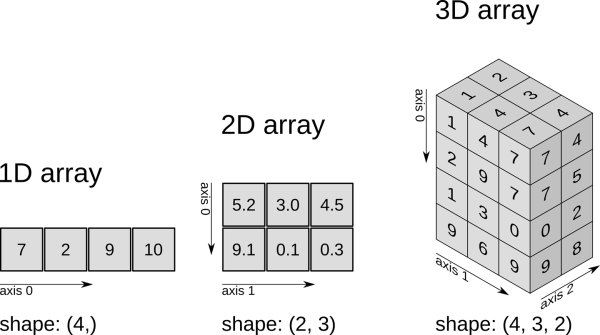
\includegraphics[keepaspectratio]{img/arrays.png}}

}

\caption{Arrays}

\end{figure}%

\section{Creación de arrays}\label{creaciuxf3n-de-arrays}

Para crear un array se utiliza la siguiente función de NumPy

\begin{itemize}
\item
  \texttt{np.array(lista)} : Crea un array a partir de la lista o tupla
  \texttt{lista} y devuelve una referencia a él. El número de
  dimensiones del array dependerá de las listas o tuplas anidadas en
  \texttt{lista}:
\item
  Para una lista de valores se crea un array de una dimensión, también
  conocido como \textbf{vector}.
\item
  Para una lista de listas de valores se crea un array de dos
  dimensiones, también conocido como \textbf{matriz}.
\item
  Para una lista de listas de listas de valores se crea un array de tres
  dimensiones, también conocido como \textbf{cubo}.
\item
  Y así sucesivamente. No hay límite en el número de dimensiones del
  array más allá de la memoria disponible en el sistema.
\end{itemize}

\begin{tcolorbox}[enhanced jigsaw, arc=.35mm, bottomrule=.15mm, bottomtitle=1mm, breakable, colback=white, colbacktitle=quarto-callout-warning-color!10!white, colframe=quarto-callout-warning-color-frame, coltitle=black, left=2mm, leftrule=.75mm, opacityback=0, opacitybacktitle=0.6, rightrule=.15mm, title=\textcolor{quarto-callout-warning-color}{\faExclamationTriangle}\hspace{0.5em}{Advertencia}, titlerule=0mm, toprule=.15mm, toptitle=1mm]

Los elementos de la lista o tupla deben ser del mismo tipo.

\end{tcolorbox}

\begin{Shaded}
\begin{Highlighting}[]
\OperatorTok{\textgreater{}\textgreater{}\textgreater{}} \CommentTok{\# Array de una dimensión}
\OperatorTok{\textgreater{}\textgreater{}\textgreater{}}\NormalTok{ a1 }\OperatorTok{=}\NormalTok{ np.array([}\DecValTok{1}\NormalTok{, }\DecValTok{2}\NormalTok{, }\DecValTok{3}\NormalTok{])}
\OperatorTok{\textgreater{}\textgreater{}\textgreater{}} \BuiltInTok{print}\NormalTok{(a1)}
\NormalTok{[}\DecValTok{1} \DecValTok{2} \DecValTok{3}\NormalTok{]}
\OperatorTok{\textgreater{}\textgreater{}\textgreater{}} \CommentTok{\# Array de dos dimensiones}
\OperatorTok{\textgreater{}\textgreater{}\textgreater{}}\NormalTok{ a2 }\OperatorTok{=}\NormalTok{ np.array([[}\DecValTok{1}\NormalTok{, }\DecValTok{2}\NormalTok{, }\DecValTok{3}\NormalTok{], [}\DecValTok{4}\NormalTok{, }\DecValTok{5}\NormalTok{, }\DecValTok{6}\NormalTok{]])}
\OperatorTok{\textgreater{}\textgreater{}\textgreater{}} \BuiltInTok{print}\NormalTok{(a2)}
\NormalTok{[[}\DecValTok{1} \DecValTok{2} \DecValTok{3}\NormalTok{]}
\NormalTok{ [}\DecValTok{4} \DecValTok{5} \DecValTok{6}\NormalTok{]]}
\OperatorTok{\textgreater{}\textgreater{}\textgreater{}} \CommentTok{\# Array de tres dimensiones}
\OperatorTok{\textgreater{}\textgreater{}\textgreater{}}\NormalTok{ a3 }\OperatorTok{=}\NormalTok{ np.array([[[}\DecValTok{1}\NormalTok{, }\DecValTok{2}\NormalTok{, }\DecValTok{3}\NormalTok{], [}\DecValTok{4}\NormalTok{, }\DecValTok{5}\NormalTok{, }\DecValTok{6}\NormalTok{]], [[}\DecValTok{7}\NormalTok{, }\DecValTok{8}\NormalTok{, }\DecValTok{9}\NormalTok{], [}\DecValTok{10}\NormalTok{, }\DecValTok{11}\NormalTok{, }\DecValTok{12}\NormalTok{]]])}
\OperatorTok{\textgreater{}\textgreater{}\textgreater{}} \BuiltInTok{print}\NormalTok{(a3)}
\NormalTok{[[[ }\DecValTok{1}  \DecValTok{2}  \DecValTok{3}\NormalTok{]}
\NormalTok{  [ }\DecValTok{4}  \DecValTok{5}  \DecValTok{6}\NormalTok{]]}

\NormalTok{ [[ }\DecValTok{7}  \DecValTok{8}  \DecValTok{9}\NormalTok{]}
\NormalTok{  [}\DecValTok{10} \DecValTok{11} \DecValTok{12}\NormalTok{]]]}
\end{Highlighting}
\end{Shaded}

Otras funciones útiles que permiten generar arrays son:

\begin{itemize}
\item
  \texttt{np.empty(dimensiones)} : Crea y devuelve una referencia a un
  array vacío con las dimensiones especificadas en la tupla
  \texttt{dimensiones}.
\item
  \texttt{np.zeros(dimensiones)} : Crea y devuelve una referencia a un
  array con las dimensiones especificadas en la tupla
  \texttt{dimensiones} cuyos elementos son todos ceros.
\item
  \texttt{np.ones(dimensiones)} : Crea y devuelve una referencia a un
  array con las dimensiones especificadas en la tupla
  \texttt{dimensiones} cuyos elementos son todos unos.
\item
  \texttt{np.full(dimensiones,\ valor)} : Crea y devuelve una referencia
  a un array con las dimensiones especificadas en la tupla
  \texttt{dimensiones} cuyos elementos son todos \texttt{valor}.
\item
  \texttt{np.identity(n)} : Crea y devuelve una referencia a la matriz
  identidad de dimensión \texttt{n}.
\item
  \texttt{np.arange(inicio,\ fin,\ salto)} : Crea y devuelve una
  referencia a un array de una dimensión cuyos elementos son la
  secuencia desde \texttt{inicio} hasta \texttt{fin} tomando valores
  cada \texttt{salto}.
\item
  \texttt{np.linspace(inicio,\ fin,\ n)} : Crea y devuelve una
  referencia a un array de una dimensión cuyos elementos son la
  secuencia de \texttt{n} valores equidistantes desde \texttt{inicio}
  hasta \texttt{fin}.
\item
  \texttt{np.random.random(dimensiones)} : Crea y devuelve una
  referencia a un array con las dimensiones especificadas en la tupla
  \texttt{dimensiones} cuyos elementos son aleatorios.
\end{itemize}

\begin{Shaded}
\begin{Highlighting}[]
\OperatorTok{\textgreater{}\textgreater{}\textgreater{}} \BuiltInTok{print}\NormalTok{(np.zeros(}\DecValTok{3}\NormalTok{,}\DecValTok{2}\NormalTok{))}
\NormalTok{[[}\FloatTok{0.} \FloatTok{0.} \FloatTok{0.}\NormalTok{]}
\NormalTok{ [}\FloatTok{0.} \FloatTok{0.} \FloatTok{0.}\NormalTok{]]}
\OperatorTok{\textgreater{}\textgreater{}\textgreater{}} \BuiltInTok{print}\NormalTok{(np.idendity(}\DecValTok{3}\NormalTok{))}
\NormalTok{[[}\FloatTok{1.} \FloatTok{0.} \FloatTok{0.}\NormalTok{]}
\NormalTok{ [}\FloatTok{0.} \FloatTok{1.} \FloatTok{0.}\NormalTok{]}
\NormalTok{ [}\FloatTok{0.} \FloatTok{0.} \FloatTok{1.}\NormalTok{]]}
\OperatorTok{\textgreater{}\textgreater{}\textgreater{}} \BuiltInTok{print}\NormalTok{(np.arange(}\DecValTok{1}\NormalTok{, }\DecValTok{10}\NormalTok{, }\DecValTok{2}\NormalTok{))}
\NormalTok{[}\DecValTok{1} \DecValTok{3} \DecValTok{5} \DecValTok{7} \DecValTok{9}\NormalTok{]}
\OperatorTok{\textgreater{}\textgreater{}\textgreater{}} \BuiltInTok{print}\NormalTok{(np.linspace(}\DecValTok{0}\NormalTok{, }\DecValTok{10}\NormalTok{, }\DecValTok{5}\NormalTok{))}
\NormalTok{[ }\FloatTok{0.}   \FloatTok{2.5}  \FloatTok{5.}   \FloatTok{7.5} \FloatTok{10.}\NormalTok{ ]}
\end{Highlighting}
\end{Shaded}

\section{Atributos de un array}\label{atributos-de-un-array}

Existen varios atributos y funciones que describen las características
de un array.

\begin{itemize}
\item
  \texttt{a.ndim} : Devuelve el número de dimensiones del array
  \texttt{a}.
\item
  \texttt{a.shape} : Devuelve una tupla con las dimensiones del array
  \texttt{a}.
\item
  \texttt{a.size} : Devuelve el número de elementos del array
  \texttt{a}.
\item
  \texttt{a.dtype}: Devuelve el tipo de datos de los elementos del array
  \texttt{a}.
\end{itemize}

\section{Acceso a los elementos de un
array}\label{acceso-a-los-elementos-de-un-array}

Para acceder a los elementos contenidos en un array se usan índices al
igual que para acceder a los elementos de una lista, pero indicando los
índices de cada dimensión separados por comas.

Al igual que para listas, los índices de cada dimensión comienzan en 0.

También es posible obtener subarrays con el operador dos puntos
\texttt{:} indicando el índice inicial y el siguiente al final para cada
dimensión, de nuevo separados por comas.

\begin{Shaded}
\begin{Highlighting}[]
\OperatorTok{\textgreater{}\textgreater{}\textgreater{}}\NormalTok{ a }\OperatorTok{=}\NormalTok{ np.array([[}\DecValTok{1}\NormalTok{, }\DecValTok{2}\NormalTok{, }\DecValTok{3}\NormalTok{], [}\DecValTok{4}\NormalTok{, }\DecValTok{5}\NormalTok{, }\DecValTok{6}\NormalTok{]])}
\OperatorTok{\textgreater{}\textgreater{}\textgreater{}} \BuiltInTok{print}\NormalTok{(a[}\DecValTok{1}\NormalTok{, }\DecValTok{0}\NormalTok{])  }\CommentTok{\# Acceso al elemento de la fila 1 columna 0}
\DecValTok{4}
\OperatorTok{\textgreater{}\textgreater{}\textgreater{}} \BuiltInTok{print}\NormalTok{(a[}\DecValTok{1}\NormalTok{][}\DecValTok{0}\NormalTok{])  }\CommentTok{\# Otra forma de acceder al mismo elemento}
\DecValTok{4}
\OperatorTok{\textgreater{}\textgreater{}\textgreater{}} \BuiltInTok{print}\NormalTok{(a[:, }\DecValTok{0}\NormalTok{:}\DecValTok{2}\NormalTok{])}
\NormalTok{[[}\DecValTok{1} \DecValTok{2}\NormalTok{]}
\NormalTok{ [}\DecValTok{4} \DecValTok{5}\NormalTok{]]}
\end{Highlighting}
\end{Shaded}

\section{Filtrado de elementos de un
array}\label{filtrado-de-elementos-de-un-array}

Una característica muy útil de los arrays es que es muy fácil obtener
otro array con los elementos que cumplen una condición.

\begin{itemize}
\item
  \texttt{a{[}condicion{]}} : Devuelve una lista con los elementos del
  array \texttt{a} que cumplen la condición \texttt{condicion}.

\begin{Shaded}
\begin{Highlighting}[]
\OperatorTok{\textgreater{}\textgreater{}\textgreater{}}\NormalTok{ a }\OperatorTok{=}\NormalTok{ np.array([[}\DecValTok{1}\NormalTok{, }\DecValTok{2}\NormalTok{, }\DecValTok{3}\NormalTok{], [}\DecValTok{4}\NormalTok{, }\DecValTok{5}\NormalTok{, }\DecValTok{6}\NormalTok{]])}
\OperatorTok{\textgreater{}\textgreater{}\textgreater{}} \BuiltInTok{print}\NormalTok{(a[(a }\OperatorTok{\%} \DecValTok{2} \OperatorTok{==} \DecValTok{0}\NormalTok{)])}
\NormalTok{[}\DecValTok{2} \DecValTok{4} \DecValTok{6}\NormalTok{]}
\OperatorTok{\textgreater{}\textgreater{}\textgreater{}} \BuiltInTok{print}\NormalTok{(a[(a }\OperatorTok{\%} \DecValTok{2} \OperatorTok{==} \DecValTok{0}\NormalTok{) }\OperatorTok{\&}\NormalTok{  (a }\OperatorTok{\textgreater{}} \DecValTok{2}\NormalTok{)])}
\NormalTok{[}\DecValTok{2} \DecValTok{4}\NormalTok{]}
\end{Highlighting}
\end{Shaded}
\end{itemize}

\section{Operaciones matemáticas con
arrays}\label{operaciones-matemuxe1ticas-con-arrays}

Existen dos formas de realizar operaciones matemáticas con arrays: a
nivel de elemento y a nivel de array.

Las operaciones a nivel de elemento operan los elementos que ocupan la
misma posición en dos arrays. Se necesitan, por tanto, dos arrays con
las mismas dimensiones y el resultado es una array de la misma
dimensión.

Los operadores mamemáticos \texttt{+}, \texttt{-}, \texttt{*},
\texttt{/}, \texttt{\%}, \texttt{**} se utilizan para la realizar suma,
resta, producto, cociente, resto y potencia a nivel de elemento.

\begin{Shaded}
\begin{Highlighting}[]
\OperatorTok{\textgreater{}\textgreater{}\textgreater{}}\NormalTok{ a }\OperatorTok{=}\NormalTok{ np.array([[}\DecValTok{1}\NormalTok{, }\DecValTok{2}\NormalTok{, }\DecValTok{3}\NormalTok{], [}\DecValTok{4}\NormalTok{, }\DecValTok{5}\NormalTok{, }\DecValTok{6}\NormalTok{]])}
\OperatorTok{\textgreater{}\textgreater{}\textgreater{}}\NormalTok{ b }\OperatorTok{=}\NormalTok{ np.array([[}\DecValTok{1}\NormalTok{, }\DecValTok{1}\NormalTok{, }\DecValTok{1}\NormalTok{], [}\DecValTok{2}\NormalTok{, }\DecValTok{2}\NormalTok{, }\DecValTok{2}\NormalTok{]])}
\OperatorTok{\textgreater{}\textgreater{}\textgreater{}} \BuiltInTok{print}\NormalTok{(a }\OperatorTok{+}\NormalTok{ b )}
\NormalTok{[[}\DecValTok{2} \DecValTok{3} \DecValTok{4}\NormalTok{]}
\NormalTok{ [}\DecValTok{6} \DecValTok{7} \DecValTok{8}\NormalTok{]]}
\OperatorTok{\textgreater{}\textgreater{}\textgreater{}} \BuiltInTok{print}\NormalTok{(a }\OperatorTok{/}\NormalTok{ b)}
\NormalTok{[[}\FloatTok{1.}  \FloatTok{2.}  \FloatTok{3.}\NormalTok{ ]}
\NormalTok{ [}\FloatTok{2.}  \FloatTok{2.5} \FloatTok{3.}\NormalTok{ ]]}
\OperatorTok{\textgreater{}\textgreater{}\textgreater{}} \BuiltInTok{print}\NormalTok{(a }\OperatorTok{**} \DecValTok{2}\NormalTok{)}
\NormalTok{[[ }\DecValTok{1}  \DecValTok{4}  \DecValTok{9}\NormalTok{]}
\NormalTok{ [}\DecValTok{16} \DecValTok{25} \DecValTok{36}\NormalTok{]]}
\end{Highlighting}
\end{Shaded}

\section{Álgebra matricial}\label{uxe1lgebra-matricial}

Numpy incorpora funciones para realizar las principales operaciones
algebraicas con vectores y matrices. La mayoría de los métodos
algebráicos se agrupan en el submódulo \texttt{linalg}.

\subsection{Producto escalar de dos
vectores}\label{producto-escalar-de-dos-vectores}

Para realizar el producto escalar de dos vectores se utiliza el operador
\texttt{@} o el siguiente método:

\begin{itemize}
\item
  \texttt{u.dot(v)}: Devuelve el producto escalar de los vectores
  \texttt{u} y \texttt{v}.

\begin{Shaded}
\begin{Highlighting}[]
\OperatorTok{\textgreater{}\textgreater{}\textgreater{}} \ImportTok{import}\NormalTok{ numpy }\ImportTok{as}\NormalTok{ np}
\OperatorTok{\textgreater{}\textgreater{}\textgreater{}}\NormalTok{ a }\OperatorTok{=}\NormalTok{ np.array([}\DecValTok{1}\NormalTok{, }\DecValTok{2}\NormalTok{, }\DecValTok{3}\NormalTok{])}
\OperatorTok{\textgreater{}\textgreater{}\textgreater{}}\NormalTok{ b }\OperatorTok{=}\NormalTok{ np.array([}\DecValTok{1}\NormalTok{, }\DecValTok{0}\NormalTok{, }\DecValTok{1}\NormalTok{])}
\OperatorTok{\textgreater{}\textgreater{}\textgreater{}} \BuiltInTok{print}\NormalTok{(a }\OperatorTok{@}\NormalTok{ b)}
\DecValTok{4}
\OperatorTok{\textgreater{}\textgreater{}\textgreater{}} \BuiltInTok{print}\NormalTok{(a.dot(b))}
\DecValTok{4}
\end{Highlighting}
\end{Shaded}
\end{itemize}

\subsection{Módulo de un vector}\label{muxf3dulo-de-un-vector}

Para calcular el módulo de un vector se utiliza el siguiente método:

\begin{itemize}
\item
  \texttt{norm(v)}: Devuelve el módulo del vector \texttt{v}.

\begin{Shaded}
\begin{Highlighting}[]
\OperatorTok{\textgreater{}\textgreater{}\textgreater{}} \ImportTok{import}\NormalTok{ numpy }\ImportTok{as}\NormalTok{ np}
\OperatorTok{\textgreater{}\textgreater{}\textgreater{}}\NormalTok{ a }\OperatorTok{=}\NormalTok{ np.array([}\DecValTok{3}\NormalTok{, }\DecValTok{4}\NormalTok{])}
\OperatorTok{\textgreater{}\textgreater{}\textgreater{}} \BuiltInTok{print}\NormalTok{(np.linalg.norm(a))}
\FloatTok{5.0}
\end{Highlighting}
\end{Shaded}
\end{itemize}

\subsection{Producto de dos matrices}\label{producto-de-dos-matrices}

Para realizar el producto matricial se utiliza el mismo operador
\texttt{@} y método que para el producto escalar de vectores:

\begin{itemize}
\item
  \texttt{a.dot(b)} : Devuelve el producto matricial de las matrices
  \texttt{a} y \texttt{b} siempre y cuando sus dimensiones sean
  compatibles.

\begin{Shaded}
\begin{Highlighting}[]
\OperatorTok{\textgreater{}\textgreater{}\textgreater{}} \ImportTok{import}\NormalTok{ numpy }\ImportTok{as}\NormalTok{ np}
\OperatorTok{\textgreater{}\textgreater{}\textgreater{}}\NormalTok{ a }\OperatorTok{=}\NormalTok{ np.array([[}\DecValTok{1}\NormalTok{, }\DecValTok{2}\NormalTok{, }\DecValTok{3}\NormalTok{], [}\DecValTok{4}\NormalTok{, }\DecValTok{5}\NormalTok{, }\DecValTok{6}\NormalTok{]])}
\OperatorTok{\textgreater{}\textgreater{}\textgreater{}}\NormalTok{ b }\OperatorTok{=}\NormalTok{ np.array([[}\DecValTok{1}\NormalTok{, }\DecValTok{1}\NormalTok{], [}\DecValTok{2}\NormalTok{, }\DecValTok{2}\NormalTok{], [}\DecValTok{3}\NormalTok{, }\DecValTok{3}\NormalTok{]])}
\OperatorTok{\textgreater{}\textgreater{}\textgreater{}} \BuiltInTok{print}\NormalTok{(a }\OperatorTok{@}\NormalTok{ b)}
\NormalTok{[[}\DecValTok{14} \DecValTok{14}\NormalTok{]}
\NormalTok{[}\DecValTok{32} \DecValTok{32}\NormalTok{]]}
\OperatorTok{\textgreater{}\textgreater{}\textgreater{}} \BuiltInTok{print}\NormalTok{(a.dot(b))}
\NormalTok{[[}\DecValTok{14} \DecValTok{14}\NormalTok{]}
\NormalTok{[}\DecValTok{32} \DecValTok{32}\NormalTok{]]}
\end{Highlighting}
\end{Shaded}
\end{itemize}

\subsection{Matriz traspuesta}\label{matriz-traspuesta}

Para trasponer una matriz se utiliza el método

\begin{itemize}
\item
  \texttt{a.T} : Devuelve la matriz traspuesta de la matriz \texttt{a}.

\begin{Shaded}
\begin{Highlighting}[]
\OperatorTok{\textgreater{}\textgreater{}\textgreater{}} \ImportTok{import}\NormalTok{ numpy }\ImportTok{as}\NormalTok{ np}
\OperatorTok{\textgreater{}\textgreater{}\textgreater{}}\NormalTok{ a }\OperatorTok{=}\NormalTok{ np.array([[}\DecValTok{1}\NormalTok{, }\DecValTok{2}\NormalTok{, }\DecValTok{3}\NormalTok{], [}\DecValTok{4}\NormalTok{, }\DecValTok{5}\NormalTok{, }\DecValTok{6}\NormalTok{]])}
\OperatorTok{\textgreater{}\textgreater{}\textgreater{}} \BuiltInTok{print}\NormalTok{(a.T)}
\NormalTok{[[}\DecValTok{1} \DecValTok{4}\NormalTok{]}
\NormalTok{[}\DecValTok{2} \DecValTok{5}\NormalTok{]}
\NormalTok{[}\DecValTok{3} \DecValTok{6}\NormalTok{]]}
\end{Highlighting}
\end{Shaded}
\end{itemize}

\subsection{Traza de una matriz}\label{traza-de-una-matriz}

La traza de una matriz cuadrada se calcula con el siguiente método:

\begin{itemize}
\item
  \texttt{a.trace()} : Devuelve la traza (suma de la diagonal principal)
  de la matriz cuadrada \texttt{a}.

\begin{Shaded}
\begin{Highlighting}[]
\OperatorTok{\textgreater{}\textgreater{}\textgreater{}} \ImportTok{import}\NormalTok{ numpy }\ImportTok{as}\NormalTok{ np}
\OperatorTok{\textgreater{}\textgreater{}\textgreater{}}\NormalTok{ a }\OperatorTok{=}\NormalTok{ np.array([[}\DecValTok{1}\NormalTok{, }\DecValTok{2}\NormalTok{, }\DecValTok{3}\NormalTok{], [}\DecValTok{4}\NormalTok{, }\DecValTok{5}\NormalTok{, }\DecValTok{6}\NormalTok{], [}\DecValTok{7}\NormalTok{, }\DecValTok{8}\NormalTok{, }\DecValTok{9}\NormalTok{]])}
\OperatorTok{\textgreater{}\textgreater{}\textgreater{}} \BuiltInTok{print}\NormalTok{(a.trace())}
\DecValTok{15}
\end{Highlighting}
\end{Shaded}
\end{itemize}

\subsection{Determinante de una
matriz}\label{determinante-de-una-matriz}

El determinante de una matriz cuadrada se calcula con la siguiente
función:

\begin{itemize}
\item
  \texttt{det(a)} : Devuelve el determinante de la matriz cuadrada
  \texttt{a}.

\begin{Shaded}
\begin{Highlighting}[]
\OperatorTok{\textgreater{}\textgreater{}\textgreater{}} \ImportTok{import}\NormalTok{ numpy }\ImportTok{as}\NormalTok{ np}
\OperatorTok{\textgreater{}\textgreater{}\textgreater{}}\NormalTok{ a }\OperatorTok{=}\NormalTok{ np.array([[}\DecValTok{1}\NormalTok{, }\DecValTok{2}\NormalTok{], [}\DecValTok{3}\NormalTok{, }\DecValTok{4}\NormalTok{]])}
\OperatorTok{\textgreater{}\textgreater{}\textgreater{}} \BuiltInTok{print}\NormalTok{(np.linalg.det(a))}
\OperatorTok{{-}}\FloatTok{2.0}
\end{Highlighting}
\end{Shaded}
\end{itemize}

\subsection{Matriz inversa}\label{matriz-inversa}

La inversa de una matriz se calcula con la siguiente función:

\begin{itemize}
\item
  \texttt{inv(a)} : Devuelve la matriz inversa de la matriz cuadrada
  \texttt{a}.

\begin{Shaded}
\begin{Highlighting}[]
\OperatorTok{\textgreater{}\textgreater{}\textgreater{}} \ImportTok{import}\NormalTok{ numpy }\ImportTok{as}\NormalTok{ np}
\OperatorTok{\textgreater{}\textgreater{}\textgreater{}}\NormalTok{ a }\OperatorTok{=}\NormalTok{ np.array([[}\DecValTok{1}\NormalTok{, }\DecValTok{2}\NormalTok{], [}\DecValTok{3}\NormalTok{, }\DecValTok{4}\NormalTok{]])}
\OperatorTok{\textgreater{}\textgreater{}\textgreater{}} \BuiltInTok{print}\NormalTok{(np.linalg.inv(a))}
\NormalTok{[[}\OperatorTok{{-}}\FloatTok{2.}   \FloatTok{1.}\NormalTok{ ]}
\NormalTok{[ }\FloatTok{1.5} \OperatorTok{{-}}\FloatTok{0.5}\NormalTok{]]}
\end{Highlighting}
\end{Shaded}
\end{itemize}

\subsection{Autovalores de una matriz}\label{autovalores-de-una-matriz}

Los autovalores de una matriz cuadrada se calculan con la siguiente
función:

\begin{itemize}
\item
  \texttt{eigvals(a)} : Devuelve los autovalores de la matriz cuadrada
  \texttt{a}.

\begin{Shaded}
\begin{Highlighting}[]
\OperatorTok{\textgreater{}\textgreater{}\textgreater{}} \ImportTok{import}\NormalTok{ numpy }\ImportTok{as}\NormalTok{ np}
\OperatorTok{\textgreater{}\textgreater{}\textgreater{}}\NormalTok{ a }\OperatorTok{=}\NormalTok{ np.array([[}\DecValTok{1}\NormalTok{, }\DecValTok{1}\NormalTok{, }\DecValTok{0}\NormalTok{], [}\DecValTok{1}\NormalTok{, }\DecValTok{2}\NormalTok{, }\DecValTok{1}\NormalTok{], [}\DecValTok{0}\NormalTok{, }\DecValTok{1}\NormalTok{, }\DecValTok{1}\NormalTok{]])}
\OperatorTok{\textgreater{}\textgreater{}\textgreater{}} \BuiltInTok{print}\NormalTok{(np.linalg.eigvals(a))}
\NormalTok{[ }\FloatTok{3.00000000e+00}  \FloatTok{1.00000000e+00} \OperatorTok{{-}}\FloatTok{3.36770206e{-}17}\NormalTok{]}
\end{Highlighting}
\end{Shaded}
\end{itemize}

\subsection{Autovectores de una
matriz}\label{autovectores-de-una-matriz}

Los autovectores de una matriz cuadrada se calculan con la siguiente
función:

\begin{itemize}
\item
  \texttt{eig(a)} : Devuelve los autovalores y los autovectores
  asociados de la matriz cuadrada \texttt{a}.

\begin{Shaded}
\begin{Highlighting}[]
\OperatorTok{\textgreater{}\textgreater{}\textgreater{}} \ImportTok{import}\NormalTok{ numpy }\ImportTok{as}\NormalTok{ np}
\OperatorTok{\textgreater{}\textgreater{}\textgreater{}}\NormalTok{ a }\OperatorTok{=}\NormalTok{ np.array([[}\DecValTok{1}\NormalTok{, }\DecValTok{1}\NormalTok{, }\DecValTok{0}\NormalTok{], [}\DecValTok{1}\NormalTok{, }\DecValTok{2}\NormalTok{, }\DecValTok{1}\NormalTok{], [}\DecValTok{0}\NormalTok{, }\DecValTok{1}\NormalTok{, }\DecValTok{1}\NormalTok{]])}
\OperatorTok{\textgreater{}\textgreater{}\textgreater{}} \BuiltInTok{print}\NormalTok{(np.linalg.eig(a))}
\NormalTok{(array([ }\FloatTok{3.00000000e+00}\NormalTok{,  }\FloatTok{1.00000000e+00}\NormalTok{, }\OperatorTok{{-}}\FloatTok{3.36770206e{-}17}\NormalTok{]), array([[}\OperatorTok{{-}}\FloatTok{4.08248290e{-}01}\NormalTok{,  }\FloatTok{7.07106781e{-}01}\NormalTok{,  }\FloatTok{5.77350269e{-}01}\NormalTok{],}
\NormalTok{      [}\OperatorTok{{-}}\FloatTok{8.16496581e{-}01}\NormalTok{,  }\FloatTok{2.61239546e{-}16}\NormalTok{, }\OperatorTok{{-}}\FloatTok{5.77350269e{-}01}\NormalTok{],}
\NormalTok{      [}\OperatorTok{{-}}\FloatTok{4.08248290e{-}01}\NormalTok{, }\OperatorTok{{-}}\FloatTok{7.07106781e{-}01}\NormalTok{,  }\FloatTok{5.77350269e{-}01}\NormalTok{]]))}
\end{Highlighting}
\end{Shaded}
\end{itemize}

\subsection{Solución de un sistema de
ecuaciones}\label{soluciuxf3n-de-un-sistema-de-ecuaciones}

Para resolver un sistema de ecuaciones lineales se utiliza la función
siguiente:

\begin{itemize}
\item
  \texttt{solve(a,\ b)} : Devuelve la solución del sistema de ecuaciones
  lineales con los coeficientes de la matriz \texttt{a} y los términos
  independientes de la matriz \texttt{b}.

\begin{Shaded}
\begin{Highlighting}[]
\OperatorTok{\textgreater{}\textgreater{}\textgreater{}} \ImportTok{import}\NormalTok{ numpy }\ImportTok{as}\NormalTok{ np}
\CommentTok{\# Sistema de dos ecuaciones y dos incógnitas}
\CommentTok{\# x + 2y = 1}
\CommentTok{\# 3x + 5y = 2 }
\OperatorTok{\textgreater{}\textgreater{}\textgreater{}}\NormalTok{ a }\OperatorTok{=}\NormalTok{ np.array([[}\DecValTok{1}\NormalTok{, }\DecValTok{2}\NormalTok{], [}\DecValTok{3}\NormalTok{, }\DecValTok{5}\NormalTok{]])}
\OperatorTok{\textgreater{}\textgreater{}\textgreater{}}\NormalTok{ b }\OperatorTok{=}\NormalTok{ np.array([}\DecValTok{1}\NormalTok{, }\DecValTok{2}\NormalTok{])}
\OperatorTok{\textgreater{}\textgreater{}\textgreater{}} \BuiltInTok{print}\NormalTok{(np.linalg.solve(a, b))}
\NormalTok{[}\OperatorTok{{-}}\FloatTok{1.}  \FloatTok{1.}\NormalTok{]}
\end{Highlighting}
\end{Shaded}
\end{itemize}

\bookmarksetup{startatroot}

\chapter{La librería Pandas}\label{la-libreruxeda-pandas}

\href{https://pandas.pydata.org}{Pandas} es una librería de Python
especializada en el manejo y análisis de estructuras de datos.

\begin{figure}[H]

{\centering \pandocbounded{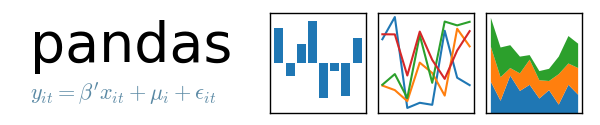
\includegraphics[keepaspectratio]{img/pandas-logo.png}}

}

\caption{Logo librería Pandas}

\end{figure}%

Las principales características de esta librería son:

\begin{itemize}
\tightlist
\item
  Define nuevas estructuras de datos basadas en los arrays de la
  librería NumPy pero con nuevas funcionalidades.
\item
  Permite leer y escribir fácilmente ficheros en formato CSV, Excel y
  bases de datos SQL.
\item
  Permite acceder a los datos mediante índices o nombres para filas y
  columnas.
\item
  Ofrece métodos para reordenar, dividir y combinar conjuntos de datos.
\item
  Permite trabajar con series temporales.
\item
  Realiza todas estas operaciones de manera muy eficiente.
\end{itemize}

\section{Tipos de datos de Pandas}\label{tipos-de-datos-de-pandas}

Pandas dispone de tres estructuras de datos diferentes:

\begin{itemize}
\tightlist
\item
  Series: Estructura de una dimensión.
\item
  DataFrame: Estructura de dos dimensiones (tablas).
\item
  Panel: Estructura de tres dimensiones (cubos).
\end{itemize}

Estas estructuras se construyen a partir de arrays de la librería NumPy,
añadiendo nuevas funcionalidades.

\section{La clase de objetos Series}\label{la-clase-de-objetos-series}

Son estructuras similares a los arrays de una dimensión. Son homogéneas,
es decir, sus elementos tienen que ser del mismo tipo, y su tamaño es
inmutable, es decir, no se puede cambiar, aunque si su contenido.

Dispone de un índice que asocia un nombre a cada elemento del la serie,
a través de la cuál se accede al elemento.

Ejemplo. La siguiente serie contiene las asignaturas de un curso.

\begin{figure}[H]

{\centering \pandocbounded{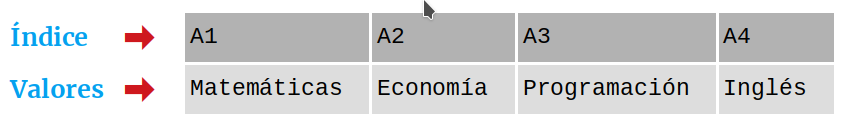
\includegraphics[keepaspectratio]{img/pandas-series.png}}

}

\caption{Ejemplo de serie}

\end{figure}%

\section{Creación de series}\label{creaciuxf3n-de-series}

\subsection{Creación de una serie a partir de una
lista}\label{creaciuxf3n-de-una-serie-a-partir-de-una-lista}

\begin{itemize}
\tightlist
\item
  \texttt{Series(data=lista,\ index=indices,\ dtype=tipo)} : Devuelve un
  objeto de tipo Series con los datos de la lista \texttt{lista}, las
  filas especificados en la lista \texttt{indices} y el tipo de datos
  indicado en \texttt{tipo}. Si no se pasa la lista de índices se
  utilizan como índices los enteros del 0 al \(n-1\), done \(n\) es el
  tamaño de la serie. Si no se pasa el tipo de dato se infiere.
\end{itemize}

\begin{Shaded}
\begin{Highlighting}[]
\OperatorTok{\textgreater{}\textgreater{}\textgreater{}} \ImportTok{import}\NormalTok{ pandas }\ImportTok{as}\NormalTok{ pd}
\OperatorTok{\textgreater{}\textgreater{}\textgreater{}}\NormalTok{ s }\OperatorTok{=}\NormalTok{ pd.Series([}\StringTok{\textquotesingle{}Matemáticas\textquotesingle{}}\NormalTok{, }\StringTok{\textquotesingle{}Historia\textquotesingle{}}\NormalTok{, }\StringTok{\textquotesingle{}Economía\textquotesingle{}}\NormalTok{, }\StringTok{\textquotesingle{}Programación\textquotesingle{}}\NormalTok{, }\StringTok{\textquotesingle{}Inglés\textquotesingle{}}\NormalTok{], dtype}\OperatorTok{=}\StringTok{\textquotesingle{}string\textquotesingle{}}\NormalTok{)}
\OperatorTok{\textgreater{}\textgreater{}\textgreater{}} \BuiltInTok{print}\NormalTok{(s)}
\DecValTok{0}\NormalTok{     Matemáticas}
\DecValTok{1}\NormalTok{        Historia}
\DecValTok{2}\NormalTok{        Economía}
\DecValTok{3}\NormalTok{    Programación}
\DecValTok{4}\NormalTok{          Inglés}
\NormalTok{dtype: string}
\end{Highlighting}
\end{Shaded}

\subsection{Creación de una serie a partir de un
diccionario}\label{creaciuxf3n-de-una-serie-a-partir-de-un-diccionario}

\begin{itemize}
\tightlist
\item
  \texttt{Series(data=diccionario,\ index=indices)}: Devuelve un objeto
  de tipo Series con los valores del diccionario \texttt{diccionario} y
  las filas especificados en la lista \texttt{indices}. Si no se pasa la
  lista de índices se utilizan como índices las claves del diccionario.
\end{itemize}

\begin{Shaded}
\begin{Highlighting}[]
\OperatorTok{\textgreater{}\textgreater{}\textgreater{}} \ImportTok{import}\NormalTok{ pandas }\ImportTok{as}\NormalTok{ pd}
\OperatorTok{\textgreater{}\textgreater{}\textgreater{}}\NormalTok{ s }\OperatorTok{=}\NormalTok{ pd.Series(\{}\StringTok{\textquotesingle{}Matemáticas\textquotesingle{}}\NormalTok{: }\FloatTok{6.0}\NormalTok{,  }\StringTok{\textquotesingle{}Economía\textquotesingle{}}\NormalTok{: }\FloatTok{4.5}\NormalTok{, }\StringTok{\textquotesingle{}Programación\textquotesingle{}}\NormalTok{: }\FloatTok{8.5}\NormalTok{\})}
\OperatorTok{\textgreater{}\textgreater{}\textgreater{}} \BuiltInTok{print}\NormalTok{(s)}
\NormalTok{Matemáticas     }\FloatTok{6.0}
\NormalTok{Economía        }\FloatTok{4.5}
\NormalTok{Programación    }\FloatTok{8.5}
\NormalTok{dtype: float64}
\end{Highlighting}
\end{Shaded}

\section{Atributos de una serie}\label{atributos-de-una-serie}

Existen varias propiedades o métodos para ver las características de una
serie.

\begin{itemize}
\item
  \texttt{s.size} : Devuelve el número de elementos de la serie
  \texttt{s}.
\item
  \texttt{s.index} : Devuelve una lista con los nombres de las filas del
  DataFrame \texttt{s}.
\item
  \texttt{s.dtype} : Devuelve el tipo de datos de los elementos de la
  serie \texttt{s}.
\end{itemize}

\begin{Shaded}
\begin{Highlighting}[]
\OperatorTok{\textgreater{}\textgreater{}\textgreater{}} \ImportTok{import}\NormalTok{ pandas }\ImportTok{as}\NormalTok{ pd}
\OperatorTok{\textgreater{}\textgreater{}\textgreater{}}\NormalTok{ s }\OperatorTok{=}\NormalTok{ pd.Series([}\DecValTok{1}\NormalTok{, }\DecValTok{2}\NormalTok{, }\DecValTok{2}\NormalTok{, }\DecValTok{3}\NormalTok{, }\DecValTok{3}\NormalTok{, }\DecValTok{3}\NormalTok{, }\DecValTok{4}\NormalTok{, }\DecValTok{4}\NormalTok{, }\DecValTok{4}\NormalTok{, }\DecValTok{4}\NormalTok{])}
\OperatorTok{\textgreater{}\textgreater{}\textgreater{}}\NormalTok{ s.size}
\DecValTok{10}
\OperatorTok{\textgreater{}\textgreater{}\textgreater{}}\NormalTok{ s.index}
\NormalTok{RangeIndex(start}\OperatorTok{=}\DecValTok{0}\NormalTok{, stop}\OperatorTok{=}\DecValTok{10}\NormalTok{, step}\OperatorTok{=}\DecValTok{1}\NormalTok{)}
\OperatorTok{\textgreater{}\textgreater{}\textgreater{}}\NormalTok{ s.dtype}
\NormalTok{dtype(}\StringTok{\textquotesingle{}int64\textquotesingle{}}\NormalTok{)}
\end{Highlighting}
\end{Shaded}

\section{Acceso a los elementos de una
serie}\label{acceso-a-los-elementos-de-una-serie}

El acceso a los elementos de un objeto del tipo Series puede ser a
través de posiciones o través de índices (nombres).

\subsection{Acceso por posición}\label{acceso-por-posiciuxf3n}

Se realiza de forma similar a como se accede a los elementos de un
array.

\begin{itemize}
\tightlist
\item
  \texttt{s{[}i{]}} : Devuelve el elemento que ocupa la posición
  \texttt{i+1} en la serie \texttt{s}.
\item
  \texttt{s{[}posiciones{]}}: Devuelve otra serie con los elementos que
  ocupan las posiciones de la lista \texttt{posiciones}.
\end{itemize}

\subsection{Acceso por índice}\label{acceso-por-uxedndice}

\begin{itemize}
\tightlist
\item
  \texttt{s{[}nombre{]}} : Devuelve el elemento con el nombre
  \texttt{nombre} en el índice.
\item
  \texttt{s{[}nombres{]}} : Devuelve otra serie con los elementos
  correspondientes a los nombres indicadas en la lista \texttt{nombres}
  en el índice.
\end{itemize}

\begin{Shaded}
\begin{Highlighting}[]
\OperatorTok{\textgreater{}\textgreater{}\textgreater{}}\NormalTok{ s[}\DecValTok{1}\NormalTok{:}\DecValTok{3}\NormalTok{]}
\NormalTok{Economía        }\FloatTok{4.5}
\NormalTok{Programación    }\FloatTok{8.5}
\NormalTok{dtype: float64}
\OperatorTok{\textgreater{}\textgreater{}\textgreater{}}\NormalTok{ s[}\StringTok{\textquotesingle{}Economía\textquotesingle{}}\NormalTok{]}
\FloatTok{4.5}
\OperatorTok{\textgreater{}\textgreater{}\textgreater{}}\NormalTok{ s[[}\StringTok{\textquotesingle{}Programación\textquotesingle{}}\NormalTok{, }\StringTok{\textquotesingle{}Matemáticas\textquotesingle{}}\NormalTok{]]}
\NormalTok{Programación    }\FloatTok{8.5}
\NormalTok{Matemáticas     }\FloatTok{6.0}
\NormalTok{dtype: float64}
\end{Highlighting}
\end{Shaded}

\section{Resumen descriptivo de una
serie}\label{resumen-descriptivo-de-una-serie}

Las siguientes funciones permiten resumir varios aspectos de una serie:

\begin{itemize}
\tightlist
\item
  \texttt{s.count()} : Devuelve el número de elementos que no son nulos
  ni \texttt{NaN} en la serie \texttt{s}.
\item
  \texttt{s.sum()} : Devuelve la suma de los datos de la serie
  \texttt{s} cuando los datos son de un tipo numérico, o la
  concatenación de ellos cuando son del tipo cadena \texttt{str}.
\item
  \texttt{s.cumsum()} : Devuelve una serie con la suma acumulada de los
  datos de la serie \texttt{s} cuando los datos son de un tipo numérico.
\item
  \texttt{s.value\_counts()} : Devuelve una serie con la frecuencia
  (número de repeticiones) de cada valor de la serie \texttt{s}.
\item
  \texttt{s.min()} : Devuelve el menor de los datos de la serie
  \texttt{s}.
\item
  \texttt{s.max()} : Devuelve el mayor de los datos de la serie
  \texttt{s}.
\item
  \texttt{s.mean()} : Devuelve la media de los datos de la serie
  \texttt{s} cuando los datos son de un tipo numérico.
\item
  \texttt{s.var()} : Devuelve la varianza de los datos de la serie
  \texttt{s} cuando los datos son de un tipo numérico.
\item
  \texttt{s.std()} : Devuelve la desviación típica de los datos de la
  serie \texttt{s} cuando los datos son de un tipo numérico.
\item
  \texttt{s.describe()}: Devuelve una serie con un resumen descriptivo
  que incluye el número de datos, su suma, el mínimo, el máximo, la
  media, la desviación típica y los cuartiles.
\end{itemize}

\begin{Shaded}
\begin{Highlighting}[]
\OperatorTok{\textgreater{}\textgreater{}\textgreater{}} \ImportTok{import}\NormalTok{ pandas }\ImportTok{as}\NormalTok{ pd}
\OperatorTok{\textgreater{}\textgreater{}\textgreater{}}\NormalTok{ s }\OperatorTok{=}\NormalTok{ pd.Series([}\DecValTok{1}\NormalTok{, }\DecValTok{1}\NormalTok{, }\DecValTok{1}\NormalTok{, }\DecValTok{1}\NormalTok{, }\DecValTok{2}\NormalTok{, }\DecValTok{2}\NormalTok{, }\DecValTok{2}\NormalTok{, }\DecValTok{3}\NormalTok{, }\DecValTok{3}\NormalTok{, }\DecValTok{4}\NormalTok{])}
\OperatorTok{\textgreater{}\textgreater{}\textgreater{}}\NormalTok{ s.count()  }\CommentTok{\# Tamaño muestral}
\DecValTok{10}
\OperatorTok{\textgreater{}\textgreater{}\textgreater{}}\NormalTok{ s.}\BuiltInTok{sum}\NormalTok{()  }\CommentTok{\# Suma}
\DecValTok{20}
\OperatorTok{\textgreater{}\textgreater{}\textgreater{}}\NormalTok{ s.cumsum()  }\CommentTok{\# Suma acumulada}
\DecValTok{0}     \DecValTok{1}
\DecValTok{1}     \DecValTok{2}
\DecValTok{2}     \DecValTok{3}
\DecValTok{3}     \DecValTok{4}
\DecValTok{4}     \DecValTok{6}
\DecValTok{5}     \DecValTok{8}
\DecValTok{6}    \DecValTok{10}
\DecValTok{7}    \DecValTok{13}
\DecValTok{8}    \DecValTok{16}
\DecValTok{9}    \DecValTok{20}
\NormalTok{dtype: int64}
\OperatorTok{\textgreater{}\textgreater{}\textgreater{}}\NormalTok{ s.value\_counts()  }\CommentTok{\# Frecuencias absolutas}
\DecValTok{1}    \DecValTok{4}
\DecValTok{2}    \DecValTok{3}
\DecValTok{3}    \DecValTok{2}
\DecValTok{4}    \DecValTok{1}
\NormalTok{dtype: int64}
\OperatorTok{\textgreater{}\textgreater{}\textgreater{}}\NormalTok{ s.value\_counts(normalize}\OperatorTok{=}\VariableTok{True}\NormalTok{)  }\CommentTok{\# Frecuencias relativas}
\DecValTok{1}    \FloatTok{0.4}
\DecValTok{2}    \FloatTok{0.3}
\DecValTok{3}    \FloatTok{0.2}
\DecValTok{4}    \FloatTok{0.1}
\NormalTok{dtype: float64}
\OperatorTok{\textgreater{}\textgreater{}\textgreater{}}\NormalTok{ s.}\BuiltInTok{min}\NormalTok{()  }\CommentTok{\# Mínimo}
\DecValTok{1}
\OperatorTok{\textgreater{}\textgreater{}\textgreater{}}\NormalTok{ s.}\BuiltInTok{max}\NormalTok{()  }\CommentTok{\# Máximo}
\DecValTok{4}
\OperatorTok{\textgreater{}\textgreater{}\textgreater{}}\NormalTok{ s.mean()  }\CommentTok{\# Media}
\FloatTok{2.0}
\OperatorTok{\textgreater{}\textgreater{}\textgreater{}}\NormalTok{ s.var()  }\CommentTok{\# Varianza}
\FloatTok{1.1111111111111112}
\OperatorTok{\textgreater{}\textgreater{}\textgreater{}}\NormalTok{ s.std()  }\CommentTok{\# Desviación típica}
\FloatTok{1.0540925533894598}
\OperatorTok{\textgreater{}\textgreater{}\textgreater{}}\NormalTok{ s.describe()  }\CommentTok{\# Resume descriptivo}
\NormalTok{count    }\FloatTok{10.000000}
\NormalTok{mean      }\FloatTok{2.000000}
\NormalTok{std       }\FloatTok{1.054093}
\BuiltInTok{min}       \FloatTok{1.000000}
\DecValTok{25}\OperatorTok{\%}       \FloatTok{1.000000}
\DecValTok{50}\OperatorTok{\%}       \FloatTok{2.000000}
\DecValTok{75}\OperatorTok{\%}       \FloatTok{2.750000}
\BuiltInTok{max}       \FloatTok{4.000000}
\NormalTok{dtype: float64}
\end{Highlighting}
\end{Shaded}

\section{Aplicar operaciones a una
serie}\label{aplicar-operaciones-a-una-serie}

Los operadores binarios (\texttt{+}, \texttt{*}, \texttt{/}, etc.)
pueden utilizarse con una serie, y devuelven otra serie con el resultado
de aplicar la operación a cada elemento de la serie.

\begin{Shaded}
\begin{Highlighting}[]
\OperatorTok{\textgreater{}\textgreater{}\textgreater{}} \ImportTok{import}\NormalTok{ pandas }\ImportTok{as}\NormalTok{ pd}
\NormalTok{s }\OperatorTok{=}\NormalTok{ pd.Series([}\DecValTok{1}\NormalTok{, }\DecValTok{2}\NormalTok{, }\DecValTok{3}\NormalTok{, }\DecValTok{4}\NormalTok{])}
\OperatorTok{\textgreater{}\textgreater{}\textgreater{}}\NormalTok{ s }\OperatorTok{*} \DecValTok{2}
\DecValTok{0}    \DecValTok{2}
\DecValTok{1}    \DecValTok{4}
\DecValTok{2}    \DecValTok{6}
\DecValTok{3}    \DecValTok{8}
\NormalTok{dtype: int64}
\OperatorTok{\textgreater{}\textgreater{}\textgreater{}}\NormalTok{ s }\OperatorTok{\%} \DecValTok{2}
\DecValTok{0}    \DecValTok{1}
\DecValTok{1}    \DecValTok{0}
\DecValTok{2}    \DecValTok{1}
\DecValTok{3}    \DecValTok{0}
\NormalTok{dtype: int64}
\OperatorTok{\textgreater{}\textgreater{}\textgreater{}}\NormalTok{ s }\OperatorTok{=}\NormalTok{ pd.Series([}\StringTok{\textquotesingle{}a\textquotesingle{}}\NormalTok{, }\StringTok{\textquotesingle{}b\textquotesingle{}}\NormalTok{, }\StringTok{\textquotesingle{}c\textquotesingle{}}\NormalTok{])}
\OperatorTok{\textgreater{}\textgreater{}\textgreater{}}\NormalTok{ s }\OperatorTok{*} \DecValTok{5}
\DecValTok{0}\NormalTok{    aaaaa}
\DecValTok{1}\NormalTok{    bbbbb}
\DecValTok{2}\NormalTok{    ccccc}
\NormalTok{dtype: }\BuiltInTok{object}
\end{Highlighting}
\end{Shaded}

\section{Aplicar funciones a una
serie}\label{aplicar-funciones-a-una-serie}

También es posible aplicar una función a cada elemento de la serie
mediante el siguiente método:

\begin{itemize}
\tightlist
\item
  \texttt{s.apply(f)} : Devuelve una serie con el resultado de aplicar
  la función \texttt{f} a cada uno de los elementos de la serie
  \texttt{s}.
\end{itemize}

\begin{Shaded}
\begin{Highlighting}[]
\OperatorTok{\textgreater{}\textgreater{}\textgreater{}} \ImportTok{import}\NormalTok{ pandas }\ImportTok{as}\NormalTok{ pd}
\OperatorTok{\textgreater{}\textgreater{}\textgreater{}} \ImportTok{from}\NormalTok{ math }\ImportTok{import}\NormalTok{ log}
\OperatorTok{\textgreater{}\textgreater{}\textgreater{}}\NormalTok{ s }\OperatorTok{=}\NormalTok{ pd.Series([}\DecValTok{1}\NormalTok{, }\DecValTok{2}\NormalTok{, }\DecValTok{3}\NormalTok{, }\DecValTok{4}\NormalTok{])}
\OperatorTok{\textgreater{}\textgreater{}\textgreater{}}\NormalTok{ s.}\BuiltInTok{apply}\NormalTok{(log)}
\DecValTok{0}    \FloatTok{0.000000}
\DecValTok{1}    \FloatTok{0.693147}
\DecValTok{2}    \FloatTok{1.098612}
\DecValTok{3}    \FloatTok{1.386294}
\NormalTok{dtype: float64}
\OperatorTok{\textgreater{}\textgreater{}\textgreater{}}\NormalTok{ s }\OperatorTok{=}\NormalTok{ pd.Series([}\StringTok{\textquotesingle{}a\textquotesingle{}}\NormalTok{, }\StringTok{\textquotesingle{}b\textquotesingle{}}\NormalTok{, }\StringTok{\textquotesingle{}c\textquotesingle{}}\NormalTok{])}
\OperatorTok{\textgreater{}\textgreater{}\textgreater{}}\NormalTok{ s.}\BuiltInTok{apply}\NormalTok{(}\BuiltInTok{str}\NormalTok{.upper)}
\DecValTok{0}\NormalTok{    A}
\DecValTok{1}\NormalTok{    B}
\DecValTok{2}\NormalTok{    C}
\NormalTok{dtype: }\BuiltInTok{object}
\end{Highlighting}
\end{Shaded}

\section{Filtrar una serie}\label{filtrar-una-serie}

Para filtrar una serie y quedarse con los valores que cumplen una
determinada condición se utiliza el siguiente método:

\begin{itemize}
\tightlist
\item
  \texttt{s{[}condicion{]}} : Devuelve una serie con los elementos de la
  serie \texttt{s} que se corresponden con el valor \texttt{True} de la
  lista booleana \texttt{condicion}. \texttt{condicion} debe ser una
  lista de valores booleanos de la misma longitud que la serie.
\end{itemize}

\begin{Shaded}
\begin{Highlighting}[]
\OperatorTok{\textgreater{}\textgreater{}\textgreater{}} \ImportTok{import}\NormalTok{ pandas }\ImportTok{as}\NormalTok{ pd}
\OperatorTok{\textgreater{}\textgreater{}\textgreater{}}\NormalTok{ s }\OperatorTok{=}\NormalTok{ pd.Series(\{}\StringTok{\textquotesingle{}Matemáticas\textquotesingle{}}\NormalTok{: }\FloatTok{6.0}\NormalTok{,  }\StringTok{\textquotesingle{}Economía\textquotesingle{}}\NormalTok{: }\FloatTok{4.5}\NormalTok{, }\StringTok{\textquotesingle{}Programación\textquotesingle{}}\NormalTok{: }\FloatTok{8.5}\NormalTok{\})}
\OperatorTok{\textgreater{}\textgreater{}\textgreater{}} \BuiltInTok{print}\NormalTok{(s[s }\OperatorTok{\textgreater{}} \DecValTok{5}\NormalTok{])}
\NormalTok{Matemáticas     }\FloatTok{6.0}
\NormalTok{Programación    }\FloatTok{8.5}
\NormalTok{dtype: float64}
\end{Highlighting}
\end{Shaded}

\section{Ordenar una serie}\label{ordenar-una-serie}

Para ordenar una serie se utilizan los siguientes métodos:

\begin{itemize}
\item
  \texttt{s.sort\_values(ascending=booleano}) : Devuelve la serie que
  resulta de ordenar los valores la serie \texttt{s}. Si argumento del
  parámetro \texttt{ascending} es \texttt{True} el orden es creciente y
  si es \texttt{False} decreciente.
\item
  \texttt{df.sort\_index(ascending=booleano}) : Devuelve la serie que
  resulta de ordenar el índice de la serie \texttt{s}. Si el argumento
  del parámetro \texttt{ascending} es \texttt{True} el orden es
  creciente y si es \texttt{False} decreciente.
\end{itemize}

\begin{Shaded}
\begin{Highlighting}[]
\OperatorTok{\textgreater{}\textgreater{}\textgreater{}} \ImportTok{import}\NormalTok{ pandas }\ImportTok{as}\NormalTok{ pd}
\OperatorTok{\textgreater{}\textgreater{}\textgreater{}}\NormalTok{ s }\OperatorTok{=}\NormalTok{ pd.Series(\{}\StringTok{\textquotesingle{}Matemáticas\textquotesingle{}}\NormalTok{: }\FloatTok{6.0}\NormalTok{,  }\StringTok{\textquotesingle{}Economía\textquotesingle{}}\NormalTok{: }\FloatTok{4.5}\NormalTok{, }\StringTok{\textquotesingle{}Programación\textquotesingle{}}\NormalTok{: }\FloatTok{8.5}\NormalTok{\})}
\OperatorTok{\textgreater{}\textgreater{}\textgreater{}} \BuiltInTok{print}\NormalTok{(s.sort\_values())}
\NormalTok{Economía        }\FloatTok{4.5}
\NormalTok{Matemáticas     }\FloatTok{6.0}
\NormalTok{Programación    }\FloatTok{8.5}
\NormalTok{dtype: float64}
\OperatorTok{\textgreater{}\textgreater{}\textgreater{}} \BuiltInTok{print}\NormalTok{(s.sort\_index(ascending }\OperatorTok{=} \VariableTok{False}\NormalTok{))}
\NormalTok{Programación    }\FloatTok{8.5}
\NormalTok{Matemáticas     }\FloatTok{6.0}
\NormalTok{Economía        }\FloatTok{4.5}
\NormalTok{dtype: float64}
\end{Highlighting}
\end{Shaded}

\section{Eliminar los dados desconocidos en una
serie}\label{eliminar-los-dados-desconocidos-en-una-serie}

Los datos desconocidos representan en Pandas por \texttt{NaN} y los
nulos por \texttt{None}. Tanto unos como otros suelen ser un problema a
la hora de realizar algunos análisis de datos, por lo que es habitual
eliminarlos. Para eliminarlos de una serie se utiliza el siguiente
método:

\begin{itemize}
\tightlist
\item
  \texttt{s.dropna()} : Elimina los datos desconocidos o nulos de la
  serie \texttt{s}.
\end{itemize}

\begin{Shaded}
\begin{Highlighting}[]
\OperatorTok{\textgreater{}\textgreater{}\textgreater{}} \ImportTok{import}\NormalTok{ pandas }\ImportTok{as}\NormalTok{ pd}
\OperatorTok{\textgreater{}\textgreater{}\textgreater{}} \ImportTok{import}\NormalTok{ numpy }\ImportTok{as}\NormalTok{ np}
\OperatorTok{\textgreater{}\textgreater{}\textgreater{}}\NormalTok{ s }\OperatorTok{=}\NormalTok{ pd.Series([}\StringTok{\textquotesingle{}a\textquotesingle{}}\NormalTok{, }\StringTok{\textquotesingle{}b\textquotesingle{}}\NormalTok{, }\VariableTok{None}\NormalTok{, }\StringTok{\textquotesingle{}c\textquotesingle{}}\NormalTok{, np.NaN,  }\StringTok{\textquotesingle{}d\textquotesingle{}}\NormalTok{])}
\OperatorTok{\textgreater{}\textgreater{}\textgreater{}}\NormalTok{ s}
\DecValTok{0}\NormalTok{       a}
\DecValTok{1}\NormalTok{       b}
\DecValTok{2}    \VariableTok{None}
\DecValTok{3}\NormalTok{       c}
\DecValTok{4}\NormalTok{     NaN}
\DecValTok{5}\NormalTok{       d}
\NormalTok{dtype: }\BuiltInTok{object}
\OperatorTok{\textgreater{}\textgreater{}\textgreater{}}\NormalTok{ s.dropna()}
\DecValTok{0}\NormalTok{    a}
\DecValTok{1}\NormalTok{    b}
\DecValTok{3}\NormalTok{    c}
\DecValTok{5}\NormalTok{    d}
\NormalTok{dtype: }\BuiltInTok{object}
\end{Highlighting}
\end{Shaded}

\section{La clase de objetos
DataFrame}\label{la-clase-de-objetos-dataframe}

Un objeto del tipo DataFrame define un conjunto de datos estructurado en
forma de tabla donde cada columna es un objeto de tipo Series, es decir,
todos los datos de una misma columna son del mismo tipo, y las filas son
registros que pueden contender datos de distintos tipos.

Un DataFrame contiene dos índices, uno para las filas y otro para las
columnas, y se puede acceder a sus elementos mediante los nombres de las
filas y las columnas.

\textbf{Ejemplo}. El siguiente DataFrame contiene información sobre los
alumnos de un curso. Cada fila corresponde a un alumno y cada columna a
una variable.

\begin{figure}[H]

{\centering \pandocbounded{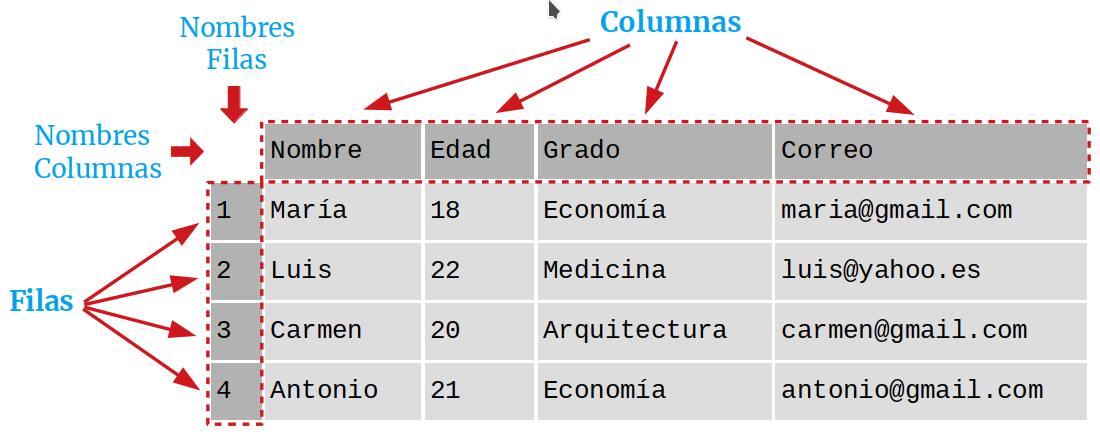
\includegraphics[keepaspectratio]{img/pandas-dataframe.png}}

}

\caption{Ejemplo de DataFrame}

\end{figure}%

\section{Creación de un DataFrame}\label{creaciuxf3n-de-un-dataframe}

\subsection{Creación de un DataFrame a partir de un diccionario de
listas}\label{creaciuxf3n-de-un-dataframe-a-partir-de-un-diccionario-de-listas}

Para crear un DataFrame a partir de un diccionario cuyas claves son los
nombres de las columnas y los valores son listas con los datos de las
columnas se utiliza el método:

\begin{itemize}
\tightlist
\item
  \texttt{DataFrame(data=diccionario,\ index=filas,\ columns=columnas,\ dtype=tipos)}
  : Devuelve un objeto del tipo DataFrame cuyas columnas son las listas
  contenidas en los valores del diccionario \texttt{diccionario}, los
  nombres de filas indicados en la lista \texttt{filas}, los nombres de
  columnas indicados en la lista \texttt{columnas} y los tipos indicados
  en la lista \texttt{tipos}. La lista \texttt{filas} tiene que tener el
  mismo tamaño que las listas del diccionario, mientras que las listas
  \texttt{columnas} y \texttt{tipos} tienen que tener el mismo tamaño
  que el diccionario. Si no se pasa la lista de filas se utilizan como
  nombres los enteros empezando en 0. Si no se pasa la lista de columnas
  se utilizan como nombres las claves del diccionario. Si no se pasa la
  lista de tipos, se infiere.
\end{itemize}

\begin{tcolorbox}[enhanced jigsaw, arc=.35mm, bottomrule=.15mm, bottomtitle=1mm, breakable, colback=white, colbacktitle=quarto-callout-warning-color!10!white, colframe=quarto-callout-warning-color-frame, coltitle=black, left=2mm, leftrule=.75mm, opacityback=0, opacitybacktitle=0.6, rightrule=.15mm, title=\textcolor{quarto-callout-warning-color}{\faExclamationTriangle}\hspace{0.5em}{Advertencia}, titlerule=0mm, toprule=.15mm, toptitle=1mm]

Los valores asociados a las claves del diccionario deben ser listas del
mismo tamaño.

\end{tcolorbox}

\begin{Shaded}
\begin{Highlighting}[]
\OperatorTok{\textgreater{}\textgreater{}\textgreater{}} \ImportTok{import}\NormalTok{ pandas }\ImportTok{as}\NormalTok{ pd}
\OperatorTok{\textgreater{}\textgreater{}\textgreater{}}\NormalTok{ datos }\OperatorTok{=}\NormalTok{ \{}\StringTok{\textquotesingle{}nombre\textquotesingle{}}\NormalTok{:[}\StringTok{\textquotesingle{}María\textquotesingle{}}\NormalTok{, }\StringTok{\textquotesingle{}Luis\textquotesingle{}}\NormalTok{, }\StringTok{\textquotesingle{}Carmen\textquotesingle{}}\NormalTok{, }\StringTok{\textquotesingle{}Antonio\textquotesingle{}}\NormalTok{],}
\NormalTok{... }\StringTok{\textquotesingle{}edad\textquotesingle{}}\NormalTok{:[}\DecValTok{18}\NormalTok{, }\DecValTok{22}\NormalTok{, }\DecValTok{20}\NormalTok{, }\DecValTok{21}\NormalTok{],}
\NormalTok{... }\StringTok{\textquotesingle{}grado\textquotesingle{}}\NormalTok{:[}\StringTok{\textquotesingle{}Economía\textquotesingle{}}\NormalTok{, }\StringTok{\textquotesingle{}Medicina\textquotesingle{}}\NormalTok{, }\StringTok{\textquotesingle{}Arquitectura\textquotesingle{}}\NormalTok{, }\StringTok{\textquotesingle{}Economía\textquotesingle{}}\NormalTok{],}
\NormalTok{... }\StringTok{\textquotesingle{}correo\textquotesingle{}}\NormalTok{:[}\StringTok{\textquotesingle{}maria@gmail.com\textquotesingle{}}\NormalTok{, }\StringTok{\textquotesingle{}luis@yahoo.es\textquotesingle{}}\NormalTok{, }\StringTok{\textquotesingle{}carmen@gmail.com\textquotesingle{}}\NormalTok{, }\StringTok{\textquotesingle{}antonio@gmail.com\textquotesingle{}}\NormalTok{]}
\NormalTok{... \}}
\OperatorTok{\textgreater{}\textgreater{}\textgreater{}}\NormalTok{ df }\OperatorTok{=}\NormalTok{ pd.DataFrame(datos)}
\OperatorTok{\textgreater{}\textgreater{}\textgreater{}} \BuiltInTok{print}\NormalTok{(df)}
\NormalTok{    nombre  edad         grado             correo}
\DecValTok{0}\NormalTok{    María    }\DecValTok{18}\NormalTok{      Economía    maria}\OperatorTok{@}\NormalTok{gmail.com}
\DecValTok{1}\NormalTok{     Luis    }\DecValTok{22}\NormalTok{      Medicina      luis}\OperatorTok{@}\NormalTok{yahoo.es}
\DecValTok{2}\NormalTok{   Carmen    }\DecValTok{20}\NormalTok{  Arquitectura   carmen}\OperatorTok{@}\NormalTok{gmail.com}
\DecValTok{3}\NormalTok{  Antonio    }\DecValTok{21}\NormalTok{      Economía  antonio}\OperatorTok{@}\NormalTok{gmail.com}
\end{Highlighting}
\end{Shaded}

\subsection{Creación de un DataFrame a partir de una lista de
listas}\label{creaciuxf3n-de-un-dataframe-a-partir-de-una-lista-de-listas}

Para crear un DataFrame a partir de una lista de listas con los datos de
las columnas se utiliza el siguiente método:

\begin{itemize}
\tightlist
\item
  \texttt{DataFrame(data=listas,\ index=filas,\ columns=columnas,\ dtype=tipos)}
  : Devuelve un objeto del tipo DataFrame cuyas columnas son los valores
  de las listas de la lista \texttt{listas}, los nombres de filas
  indicados en la lista \texttt{filas}, los nombres de columnas
  indicados en la lista \texttt{columnas} y los tipos indicados en la
  lista \texttt{tipos}. La lista \texttt{filas}, tiene que tener el
  mismo tamaño que la lista \texttt{listas} mientras que las listas
  \texttt{columnas} y \texttt{tipos} tienen que tener el mismo tamaño
  que las listas anidadas en \texttt{listas}. Si no se pasa la lista de
  filas o de columnas se utilizan enteros empezando en 0. Si no se pasa
  la lista de tipos, se infiere.
\end{itemize}

\begin{tcolorbox}[enhanced jigsaw, arc=.35mm, bottomrule=.15mm, bottomtitle=1mm, breakable, colback=white, colbacktitle=quarto-callout-warning-color!10!white, colframe=quarto-callout-warning-color-frame, coltitle=black, left=2mm, leftrule=.75mm, opacityback=0, opacitybacktitle=0.6, rightrule=.15mm, title=\textcolor{quarto-callout-warning-color}{\faExclamationTriangle}\hspace{0.5em}{Advertencia}, titlerule=0mm, toprule=.15mm, toptitle=1mm]

Si las listas anidadas en \texttt{listas} no tienen el mismo tamaño, las
listas menores se rellenan con valores \texttt{NaN}.

\end{tcolorbox}

\begin{Shaded}
\begin{Highlighting}[]
\OperatorTok{\textgreater{}\textgreater{}\textgreater{}} \ImportTok{import}\NormalTok{ pandas }\ImportTok{as}\NormalTok{ pd}
\OperatorTok{\textgreater{}\textgreater{}\textgreater{}}\NormalTok{ df }\OperatorTok{=}\NormalTok{ pd.DataFrame([[}\StringTok{\textquotesingle{}María\textquotesingle{}}\NormalTok{, }\DecValTok{18}\NormalTok{], [}\StringTok{\textquotesingle{}Luis\textquotesingle{}}\NormalTok{, }\DecValTok{22}\NormalTok{], [}\StringTok{\textquotesingle{}Carmen\textquotesingle{}}\NormalTok{, }\DecValTok{20}\NormalTok{]], columns}\OperatorTok{=}\NormalTok{[}\StringTok{\textquotesingle{}Nombre\textquotesingle{}}\NormalTok{, }\StringTok{\textquotesingle{}Edad\textquotesingle{}}\NormalTok{])}
\OperatorTok{\textgreater{}\textgreater{}\textgreater{}} \BuiltInTok{print}\NormalTok{(df)}
\NormalTok{   Nombre   Edad}
\DecValTok{0}\NormalTok{   María     }\DecValTok{18}
\DecValTok{1}\NormalTok{    Luis     }\DecValTok{22}
\DecValTok{2}\NormalTok{  Carmen     }\DecValTok{20}
\end{Highlighting}
\end{Shaded}

\subsection{Creación de un DataFrame a partir de una lista de
diccionarios}\label{creaciuxf3n-de-un-dataframe-a-partir-de-una-lista-de-diccionarios}

Para crear un DataFrame a partir de una lista de diccionarios con los
datos de las filas, se utiliza el siguiente método:

\begin{itemize}
\tightlist
\item
  \texttt{DataFrame(data=diccionarios,\ index=filas,\ columns=columnas,\ dtype=tipos)}
  : Devuelve un objeto del tipo DataFrame cuyas filas contienen los
  valores de los diccionarios de la lista \texttt{diccionarios}, los
  nombres de filas indicados en la lista \texttt{filas}, los nombres de
  columnas indicados en la lista \texttt{columnas} y los tipos indicados
  en la lista \texttt{tipos}. La lista \texttt{filas} tiene que tener el
  mismo tamaño que la lista \texttt{lista}. Si no se pasa la lista de
  filas se utilizan enteros empezando en 0. Si no se pasa la lista de
  columnas se utilizan las claves de los diccionarios. Si no se pasa la
  lista de tipos, se infiere.
\end{itemize}

\begin{tcolorbox}[enhanced jigsaw, arc=.35mm, bottomrule=.15mm, bottomtitle=1mm, breakable, colback=white, colbacktitle=quarto-callout-warning-color!10!white, colframe=quarto-callout-warning-color-frame, coltitle=black, left=2mm, leftrule=.75mm, opacityback=0, opacitybacktitle=0.6, rightrule=.15mm, title=\textcolor{quarto-callout-warning-color}{\faExclamationTriangle}\hspace{0.5em}{Advertencia}, titlerule=0mm, toprule=.15mm, toptitle=1mm]

Si los diccionarios no tienen las mismas claves, las claves que no
aparecen en el diccionario se rellenan con valores \texttt{NaN}.

\end{tcolorbox}

\begin{Shaded}
\begin{Highlighting}[]
\OperatorTok{\textgreater{}\textgreater{}\textgreater{}} \ImportTok{import}\NormalTok{ pandas }\ImportTok{as}\NormalTok{ pd}
\OperatorTok{\textgreater{}\textgreater{}\textgreater{}}\NormalTok{ df }\OperatorTok{=}\NormalTok{ pd.DataFrame([\{}\StringTok{\textquotesingle{}Nombre\textquotesingle{}}\NormalTok{:}\StringTok{\textquotesingle{}María\textquotesingle{}}\NormalTok{, }\StringTok{\textquotesingle{}Edad\textquotesingle{}}\NormalTok{:}\DecValTok{18}\NormalTok{\}, \{}\StringTok{\textquotesingle{}Nombre\textquotesingle{}}\NormalTok{:}\StringTok{\textquotesingle{}Luis\textquotesingle{}}\NormalTok{, }\StringTok{\textquotesingle{}Edad\textquotesingle{}}\NormalTok{:}\DecValTok{22}\NormalTok{\}, \{}\StringTok{\textquotesingle{}Nombre\textquotesingle{}}\NormalTok{:}\StringTok{\textquotesingle{}Carmen\textquotesingle{}}\NormalTok{\}])}
\OperatorTok{\textgreater{}\textgreater{}\textgreater{}} \BuiltInTok{print}\NormalTok{(df)}
\DecValTok{0}\NormalTok{   María  }\FloatTok{18.0}
\DecValTok{1}\NormalTok{    Luis  }\FloatTok{22.0}
\DecValTok{2}\NormalTok{  Carmen   NaN}
\end{Highlighting}
\end{Shaded}

\subsection{Creación de un DataFrame a partir de un
array}\label{creaciuxf3n-de-un-dataframe-a-partir-de-un-array}

Para crear un DataFrame a partir de un array de NumPy se utiliza el
siguiente método:

\begin{itemize}
\tightlist
\item
  \texttt{DataFrame(data=array,\ index=filas,\ columns=columnas,\ dtype=tipo)}
  : Devuelde un objeto del tipo DataFrame cuyas filas y columnas son las
  del array \texttt{array}, los nombres de filas indicados en la lista
  \texttt{filas}, los nombres de columnas indicados en la lista
  \texttt{columnas} y el tipo indicado en \texttt{tipo}. La lista
  \texttt{filas} tiene que tener el mismo tamaño que el número de filas
  del array y la lista \texttt{columnas} el mismo tamaño que el número
  de columnas del array. Si no se pasa la lista de filas se utilizan
  enteros empezando en 0. Si no se pasa la lista de columnas se utilizan
  las claves de los diccionarios. Si no se pasa la lista de tipos, se
  infiere.
\end{itemize}

\begin{Shaded}
\begin{Highlighting}[]
\OperatorTok{\textgreater{}\textgreater{}\textgreater{}} \ImportTok{import}\NormalTok{ pandas }\ImportTok{as}\NormalTok{ pd}
\OperatorTok{\textgreater{}\textgreater{}\textgreater{}}\NormalTok{ df }\OperatorTok{=}\NormalTok{ pd.DataFrame(np.random.randn(}\DecValTok{4}\NormalTok{, }\DecValTok{3}\NormalTok{), columns}\OperatorTok{=}\NormalTok{[}\StringTok{\textquotesingle{}a\textquotesingle{}}\NormalTok{, }\StringTok{\textquotesingle{}b\textquotesingle{}}\NormalTok{, }\StringTok{\textquotesingle{}c\textquotesingle{}}\NormalTok{])}
\OperatorTok{\textgreater{}\textgreater{}\textgreater{}} \BuiltInTok{print}\NormalTok{(df)}
\NormalTok{          a         b         c}
\DecValTok{0} \OperatorTok{{-}}\FloatTok{1.408238}  \FloatTok{0.644706}  \FloatTok{1.077434}
\DecValTok{1} \OperatorTok{{-}}\FloatTok{0.279264} \OperatorTok{{-}}\FloatTok{0.249229}  \FloatTok{1.019137}
\DecValTok{2} \OperatorTok{{-}}\FloatTok{0.805470} \OperatorTok{{-}}\FloatTok{0.629498}  \FloatTok{0.935066}
\DecValTok{3}  \FloatTok{0.236936} \OperatorTok{{-}}\FloatTok{0.431673} \OperatorTok{{-}}\FloatTok{0.177379}
\end{Highlighting}
\end{Shaded}

\subsection{Creación de un DataFrame a partir de un fichero CSV o
Excel}\label{creaciuxf3n-de-un-dataframe-a-partir-de-un-fichero-csv-o-excel}

Dependiendo del tipo de fichero, existen distintas funciones para
importar un DataFrame desde un fichero.

\begin{itemize}
\item
  \texttt{read\_csv(fichero.csv,\ sep=separador,\ header=n,\ index\_col=m,\ na\_values=no-validos,\ decimal=separador-decimal)}
  : Devuelve un objeto del tipo DataFrame con los datos del fichero CSV
  \texttt{fichero.csv} usando como separador de los datos la cadena
  \texttt{separador}. Como nombres de columnas se utiliza los valores de
  la fila \texttt{n} y como nombres de filas los valores de la columna
  \texttt{m}. Si no se indica \texttt{m} se utilizan como nombres de
  filas los enteros empezando en 0. Los valores incluídos en la lista
  \texttt{no-validos} se convierten en \texttt{NaN}. Para los datos
  numéricos se utiliza como separador de decimales el carácter indicado
  en \texttt{separador-decimal}.
\item
  \texttt{read\_excel(fichero.xlsx,\ sheet\_name=hoja,\ header=n,\ index\_col=m,\ na\_values=no-validos,\ decimal=separador-decimal)}
  : Devuelve un objeto del tipo DataFrame con los datos de la hoja de
  cálculo \texttt{hoja} del fichero Excel \texttt{fichero.xlsx}. Como
  nombres de columnas se utiliza los valores de la fila \texttt{n} y
  como nombres de filas los valores de la columna \texttt{m}. Si no se
  indica \texttt{m} se utilizan como nombres de filas los enteros
  empezando en 0. Los valores incluídos en la lista \texttt{no-validos}
  se convierten en \texttt{NaN}. Para los datos numéricos se utiliza
  como separador de decimales el carácter indicado en
  \texttt{separador-decimal}.
\end{itemize}

\begin{Shaded}
\begin{Highlighting}[]
\OperatorTok{\textgreater{}\textgreater{}\textgreater{}} \ImportTok{import}\NormalTok{ pandas }\ImportTok{as}\NormalTok{ pd}
\OperatorTok{\textgreater{}\textgreater{}\textgreater{}} \CommentTok{\# Importación del fichero datos{-}colesteroles.csv}
\OperatorTok{\textgreater{}\textgreater{}\textgreater{}}\NormalTok{ df }\OperatorTok{=}\NormalTok{ pd.read\_csv(}
\StringTok{\textquotesingle{}https://raw.githubusercontent.com/asalber/manual{-}python/master/datos/colesteroles.csv\textquotesingle{}}\NormalTok{, sep}\OperatorTok{=}\StringTok{\textquotesingle{};\textquotesingle{}}\NormalTok{, decimal}\OperatorTok{=}\StringTok{\textquotesingle{},\textquotesingle{}}\NormalTok{)}
\OperatorTok{\textgreater{}\textgreater{}\textgreater{}} \BuiltInTok{print}\NormalTok{(df.head())}
\NormalTok{                              nombre  edad sexo    peso    altura  colesterol}
\DecValTok{0}\NormalTok{       José Luis Martínez Izquierdo    }\DecValTok{18}\NormalTok{    H    }\FloatTok{85.0}    \FloatTok{1.79}         \FloatTok{182.0}
\DecValTok{1}\NormalTok{                     Rosa Díaz Díaz    }\DecValTok{32}\NormalTok{    M    }\FloatTok{65.0}    \FloatTok{1.73}         \FloatTok{232.0}
\DecValTok{2}\NormalTok{              Javier García Sánchez    }\DecValTok{24}\NormalTok{    H     NaN    }\FloatTok{1.81}         \FloatTok{191.0}
\DecValTok{3}\NormalTok{                Carmen López Pinzón    }\DecValTok{35}\NormalTok{    M    }\FloatTok{65.0}    \FloatTok{1.70}         \FloatTok{200.0}
\DecValTok{4}\NormalTok{               Marisa López Collado    }\DecValTok{46}\NormalTok{    M    }\FloatTok{51.0}    \FloatTok{1.58}         \FloatTok{148.0}
\end{Highlighting}
\end{Shaded}

\section{Exportación de ficheros}\label{exportaciuxf3n-de-ficheros}

También existen funciones para exportar un DataFrame a un fichero con
diferentes formatos.

\begin{itemize}
\item
  \texttt{df.to\_csv(fichero.csv,\ sep=separador,\ columns=booleano,\ index=booleano)}
  : Exporta el DataFrame \texttt{df} al fichero \texttt{fichero.csv} en
  formato CSV usando como separador de los datos la cadena
  \texttt{separador}. Si se pasa \texttt{True} al parámetro
  \texttt{columns} se exporta también la fila con los nombres de
  columnas y si se pasa \texttt{True} al parámetro \texttt{index} se
  exporta también la columna con los nombres de las filas.
\item
  \texttt{df.to\_excel(fichero.xlsx,\ sheet\_name\ =\ hoja,\ columns=booleano,\ index=booleano)}
  : Exporta el DataFrame \texttt{df} a la hoja de cálculo \texttt{hoja}
  del fichero \texttt{fichero.xlsx} en formato Excel. Si se pasa
  \texttt{True} al parámetro \texttt{columns} se exporta también la fila
  con los nombres de columnas y si se pasa \texttt{True} al parámetro
  \texttt{index} se exporta también la columna con los nombres de las
  filas.
\end{itemize}

\section{Atributos de un DataFrame}\label{atributos-de-un-dataframe}

Existen varias propiedades o métodos para ver las características de un
DataFrame.

\begin{itemize}
\item
  \texttt{df.info()} : Devuelve información (número de filas, número de
  columnas, índices, tipo de las columnas y memoria usado) sobre el
  DataFrame \texttt{df}.
\item
  \texttt{df.shape} : Devuelve una tupla con el número de filas y
  columnas del DataFrame \texttt{df}.
\item
  \texttt{df.size} : Devuelve el número de elementos del DataFrame.
\item
  \texttt{df.columns} : Devuelve una lista con los nombres de las
  columnas del DataFrame \texttt{df}.
\item
  \texttt{df.index} : Devuelve una lista con los nombres de las filas
  del DataFrame \texttt{df}.
\item
  \texttt{df.dtypes} : Devuelve una serie con los tipos de datos de las
  columnas del DataFrame \texttt{df}.
\item
  \texttt{df.head(n)} : Devuelve las \texttt{n} primeras filas del
  DataFrame \texttt{df}.
\item
  \texttt{df.tail(n)} : Devuelve las \texttt{n} últimas filas del
  DataFrame \texttt{df}.
\end{itemize}

\begin{Shaded}
\begin{Highlighting}[]
\OperatorTok{\textgreater{}\textgreater{}\textgreater{}} \ImportTok{import}\NormalTok{ pandas }\ImportTok{as}\NormalTok{ pd}
\OperatorTok{\textgreater{}\textgreater{}\textgreater{}}\NormalTok{ df }\OperatorTok{=}\NormalTok{ pd.read\_csv(}
\StringTok{\textquotesingle{}https://raw.githubusercontent.com/asalber/manual{-}python/master/datos/colesterol.csv\textquotesingle{}}\NormalTok{)}
\OperatorTok{\textgreater{}\textgreater{}\textgreater{}}\NormalTok{ df.info()}
\OperatorTok{\textless{}}\KeywordTok{class} \StringTok{\textquotesingle{}pandas.core.frame.DataFrame\textquotesingle{}}\OperatorTok{\textgreater{}}
\NormalTok{RangeIndex: }\DecValTok{14}\NormalTok{ entries, }\DecValTok{0}\NormalTok{ to }\DecValTok{13}
\NormalTok{Data columns (total }\DecValTok{6}\NormalTok{ columns):}
 \CommentTok{\#   Column      Non{-}Null Count  Dtype  }
\OperatorTok{{-}{-}{-}}  \OperatorTok{{-}{-}{-}{-}{-}{-}}      \OperatorTok{{-}{-}{-}{-}{-}{-}{-}{-}{-}{-}{-}{-}{-}{-}}  \OperatorTok{{-}{-}{-}{-}{-}}  
 \DecValTok{0}\NormalTok{   nombre      }\DecValTok{14}\NormalTok{ non}\OperatorTok{{-}}\NormalTok{null     }\BuiltInTok{object} 
 \DecValTok{1}\NormalTok{   edad        }\DecValTok{14}\NormalTok{ non}\OperatorTok{{-}}\NormalTok{null     int64  }
 \DecValTok{2}\NormalTok{   sexo        }\DecValTok{14}\NormalTok{ non}\OperatorTok{{-}}\NormalTok{null     }\BuiltInTok{object} 
 \DecValTok{3}\NormalTok{   peso        }\DecValTok{13}\NormalTok{ non}\OperatorTok{{-}}\NormalTok{null     float64}
 \DecValTok{4}\NormalTok{   altura      }\DecValTok{14}\NormalTok{ non}\OperatorTok{{-}}\NormalTok{null     float64}
 \DecValTok{5}\NormalTok{   colesterol  }\DecValTok{13}\NormalTok{ non}\OperatorTok{{-}}\NormalTok{null     float64}
\NormalTok{dtypes: float64(}\DecValTok{3}\NormalTok{), int64(}\DecValTok{1}\NormalTok{), }\BuiltInTok{object}\NormalTok{(}\DecValTok{2}\NormalTok{)}
\NormalTok{memory usage: }\FloatTok{800.0}\OperatorTok{+} \BuiltInTok{bytes}
\OperatorTok{\textgreater{}\textgreater{}\textgreater{}}\NormalTok{ df.shape}
\NormalTok{(}\DecValTok{14}\NormalTok{, }\DecValTok{6}\NormalTok{)}
\OperatorTok{\textgreater{}\textgreater{}\textgreater{}}\NormalTok{ df.size}
\DecValTok{84}
\OperatorTok{\textgreater{}\textgreater{}\textgreater{}}\NormalTok{ df.columns}
\NormalTok{Index([}\StringTok{\textquotesingle{}nombre\textquotesingle{}}\NormalTok{, }\StringTok{\textquotesingle{}edad\textquotesingle{}}\NormalTok{, }\StringTok{\textquotesingle{}sexo\textquotesingle{}}\NormalTok{, }\StringTok{\textquotesingle{}peso\textquotesingle{}}\NormalTok{, }\StringTok{\textquotesingle{}altura\textquotesingle{}}\NormalTok{, }\StringTok{\textquotesingle{}colesterol\textquotesingle{}}\NormalTok{], dtype}\OperatorTok{=}\StringTok{\textquotesingle{}object\textquotesingle{}}\NormalTok{)}
\OperatorTok{\textgreater{}\textgreater{}\textgreater{}}\NormalTok{ df.index}
\NormalTok{RangeIndex(start}\OperatorTok{=}\DecValTok{0}\NormalTok{, stop}\OperatorTok{=}\DecValTok{14}\NormalTok{, step}\OperatorTok{=}\DecValTok{1}\NormalTok{)}
\OperatorTok{\textgreater{}\textgreater{}\textgreater{}}\NormalTok{ df.dtypes}
\NormalTok{nombre         }\BuiltInTok{object}
\NormalTok{edad            int64}
\NormalTok{sexo           }\BuiltInTok{object}
\NormalTok{peso          float64}
\NormalTok{altura        float64}
\NormalTok{colesterol    float64}
\NormalTok{dtype: }\BuiltInTok{object}
\end{Highlighting}
\end{Shaded}

\section{Renombrar los nombres de las filas y
columnas}\label{renombrar-los-nombres-de-las-filas-y-columnas}

Para cambiar el nombre de las filas y las columnas de un DataFrame se
utiliza el siguiente método:

\begin{itemize}
\tightlist
\item
  \texttt{df.rename(columns=columnas,\ index=filas)}: Devuelve el
  DataFrame que resulta de renombrar las columnas indicadas en las
  claves del diccionario \texttt{columnas} con sus valores y las filas
  indicadas en las claves del diccionario \texttt{filas} con sus valores
  en el DataFrame \texttt{df}.
\end{itemize}

\begin{Shaded}
\begin{Highlighting}[]
\OperatorTok{\textgreater{}\textgreater{}\textgreater{}} \ImportTok{import}\NormalTok{ pandas }\ImportTok{as}\NormalTok{ pd}
\OperatorTok{\textgreater{}\textgreater{}\textgreater{}}\NormalTok{ df }\OperatorTok{=}\NormalTok{ pd.read\_csv(}
\StringTok{\textquotesingle{}https://raw.githubusercontent.com/asalber/manual{-}python/master/datos/colesterol.csv\textquotesingle{}}\NormalTok{)}
\OperatorTok{\textgreater{}\textgreater{}\textgreater{}} \BuiltInTok{print}\NormalTok{(df.rename(columns}\OperatorTok{=}\NormalTok{\{}\StringTok{\textquotesingle{}nombre\textquotesingle{}}\NormalTok{:}\StringTok{\textquotesingle{}nombre y apellidos\textquotesingle{}}\NormalTok{, }\StringTok{\textquotesingle{}altura\textquotesingle{}}\NormalTok{:}\StringTok{\textquotesingle{}estatura\textquotesingle{}}\NormalTok{\}, index}\OperatorTok{=}\NormalTok{\{}\DecValTok{0}\NormalTok{:}\DecValTok{1000}\NormalTok{, }\DecValTok{1}\NormalTok{:}\DecValTok{1001}\NormalTok{, }\DecValTok{2}\NormalTok{:}\DecValTok{1002}\NormalTok{\}))}
\NormalTok{                    nombre y apellidos  edad sexo    peso  estatura    colesterol}
\DecValTok{1000}\NormalTok{      José Luis Martínez Izquierdo    }\DecValTok{18}\NormalTok{    H    }\FloatTok{85.0}      \FloatTok{1.79}         \FloatTok{182.0}
\DecValTok{1001}\NormalTok{                    Rosa Díaz Díaz    }\DecValTok{32}\NormalTok{    M    }\FloatTok{65.0}      \FloatTok{1.73}         \FloatTok{232.0}
\DecValTok{1002}\NormalTok{             Javier García Sánchez    }\DecValTok{24}\NormalTok{    H     NaN      }\FloatTok{1.81}         \FloatTok{191.0}
\DecValTok{3}\NormalTok{                  Carmen López Pinzón    }\DecValTok{35}\NormalTok{    M    }\FloatTok{65.0}      \FloatTok{1.70}         \FloatTok{200.0}
\DecValTok{4}\NormalTok{                 Marisa López Collado    }\DecValTok{46}\NormalTok{    M    }\FloatTok{51.0}      \FloatTok{1.58}         \FloatTok{148.0}
\NormalTok{...}
\end{Highlighting}
\end{Shaded}

\section{Cambiar el índice de un
DataFrame}\label{cambiar-el-uxedndice-de-un-dataframe}

Aunque el índice de un DataFrame suele fijarse en la creación del mismo,
en ocasiones puede ser necesario cambiar el índice una vez creado el
DataFrame. Para ello se utiliza el siguiente método:

\begin{itemize}
\tightlist
\item
  \texttt{df.set\_index(keys\ =\ columnas,\ verify\_integrity\ =\ bool)}:
  Devuelve el DataFrame que resulta de eliminar las columnas de la lista
  \texttt{columnas} y convertirlas en el nuevo índice. El parámetro
  \texttt{verify\_integrity} recibe un booleano (\texttt{False} por
  defecto) y realiza una comprobación para evitar duplicados en la clave
  cuando recibe \texttt{True}.
\end{itemize}

\begin{Shaded}
\begin{Highlighting}[]
\OperatorTok{\textgreater{}\textgreater{}\textgreater{}} \ImportTok{import}\NormalTok{ pandas }\ImportTok{as}\NormalTok{ pd}
\OperatorTok{\textgreater{}\textgreater{}\textgreater{}}\NormalTok{ df }\OperatorTok{=}\NormalTok{ pd.read\_csv(}
\StringTok{\textquotesingle{}https://raw.githubusercontent.com/asalber/manual{-}python/master/datos/colesterol.csv\textquotesingle{}}\NormalTok{)}
\OperatorTok{\textgreater{}\textgreater{}\textgreater{}} \BuiltInTok{print}\NormalTok{(df.set\_index(}\StringTok{"nombre"}\NormalTok{).head())}
\NormalTok{                              edad sexo  peso  altura  colesterol}
\NormalTok{nombre                                                           }
\NormalTok{José Luis Martínez Izquierdo    }\DecValTok{18}\NormalTok{    H  }\FloatTok{85.0}    \FloatTok{1.79}       \FloatTok{182.0}
\NormalTok{Rosa Díaz Díaz                  }\DecValTok{32}\NormalTok{    M  }\FloatTok{65.0}    \FloatTok{1.73}       \FloatTok{232.0}
\NormalTok{Javier García Sánchez           }\DecValTok{24}\NormalTok{    H   NaN    }\FloatTok{1.81}       \FloatTok{191.0}
\NormalTok{Carmen López Pinzón             }\DecValTok{35}\NormalTok{    M  }\FloatTok{65.0}    \FloatTok{1.70}       \FloatTok{200.0}
\NormalTok{Marisa López Collado            }\DecValTok{46}\NormalTok{    M  }\FloatTok{51.0}    \FloatTok{1.58}       \FloatTok{148.0}
\OperatorTok{\textgreater{}\textgreater{}\textgreater{}} 
\end{Highlighting}
\end{Shaded}

\section{Reindexar un DataFrame}\label{reindexar-un-dataframe}

Para reordenar los índices de las filas y las columnas de un DataFrame,
así como añadir o eliminar índices, se utiliza el siguiente método:

\begin{itemize}
\tightlist
\item
  \texttt{df.reindex(index=filas,\ columns=columnas,\ fill\_value=relleno)}
  : Devuelve el DataFrame que resulta de tomar del DataFrame \texttt{df}
  las filas con nombres en la lista \texttt{filas} y las columnas con
  nombres en la lista \texttt{columnas}. Si alguno de los nombres
  indicados en \texttt{filas} o \texttt{columnas} no existía en el
  DataFrame \texttt{df}, se crean filan o columnas nuevas rellenas con
  el valor \texttt{relleno}.
\end{itemize}

\begin{Shaded}
\begin{Highlighting}[]
\OperatorTok{\textgreater{}\textgreater{}\textgreater{}} \ImportTok{import}\NormalTok{ pandas }\ImportTok{as}\NormalTok{ pd}
\OperatorTok{\textgreater{}\textgreater{}\textgreater{}}\NormalTok{ df }\OperatorTok{=}\NormalTok{ pd.read\_csv(}
\StringTok{\textquotesingle{}https://raw.githubusercontent.com/asalber/manual{-}python/master/datos/colesterol.csv\textquotesingle{}}\NormalTok{)}
\OperatorTok{\textgreater{}\textgreater{}\textgreater{}} \BuiltInTok{print}\NormalTok{(df.reindex(index}\OperatorTok{=}\NormalTok{[}\DecValTok{4}\NormalTok{, }\DecValTok{3}\NormalTok{, }\DecValTok{1}\NormalTok{], columns}\OperatorTok{=}\NormalTok{[}\StringTok{\textquotesingle{}nombre\textquotesingle{}}\NormalTok{, }\StringTok{\textquotesingle{}tensión\textquotesingle{}}\NormalTok{, }\StringTok{\textquotesingle{}colesterol\textquotesingle{}}\NormalTok{]))}
\NormalTok{                  nombre  tensión  colesterol}
\DecValTok{4}\NormalTok{   Marisa López Collado      NaN       }\FloatTok{148.0}
\DecValTok{3}\NormalTok{    Carmen López Pinzón      NaN       }\FloatTok{200.0}
\DecValTok{1}\NormalTok{         Rosa Díaz Díaz      NaN       }\FloatTok{232.0}
\end{Highlighting}
\end{Shaded}

\section{Acceso a los elementos de un
DataFrame}\label{acceso-a-los-elementos-de-un-dataframe}

El acceso a los datos de un DataFrame se puede hacer a través de
posiciones o través de los nombres de las filas y columnas.

\subsection{Accesos mediante
posiciones}\label{accesos-mediante-posiciones}

\begin{itemize}
\item
  \texttt{df.iloc{[}i,\ j{]}} : Devuelve el elemento que se encuentra en
  la fila \texttt{i} y la columna \texttt{j} del DataFrame \texttt{df}.
  Pueden indicarse secuencias de índices para obtener partes del
  DataFrame.
\item
  \texttt{df.iloc{[}filas,\ columnas{]}} : Devuelve un DataFrame con los
  elementos de las filas de la lista \texttt{filas} y de las columnas de
  la lista \texttt{columnas}.
\item
  \texttt{df.iloc{[}i{]}} : Devuelve una serie con los elementos de la
  fila \texttt{i} del DataFrame \texttt{df}.
\end{itemize}

\begin{Shaded}
\begin{Highlighting}[]
\OperatorTok{\textgreater{}\textgreater{}\textgreater{}} \ImportTok{import}\NormalTok{ pandas }\ImportTok{as}\NormalTok{ pd}
\OperatorTok{\textgreater{}\textgreater{}\textgreater{}}\NormalTok{ df }\OperatorTok{=}\NormalTok{ pd.read\_csv(}
\StringTok{\textquotesingle{}https://raw.githubusercontent.com/asalber/manual{-}python/master/datos/colesterol.csv\textquotesingle{}}\NormalTok{)}
\OperatorTok{\textgreater{}\textgreater{}\textgreater{}} \BuiltInTok{print}\NormalTok{(df.iloc[}\DecValTok{1}\NormalTok{, }\DecValTok{3}\NormalTok{])}
\DecValTok{65}
\OperatorTok{\textgreater{}\textgreater{}\textgreater{}} \BuiltInTok{print}\NormalTok{(df.iloc[}\DecValTok{1}\NormalTok{, :}\DecValTok{2}\NormalTok{])}
\NormalTok{nombre     Rosa Díaz Díaz}
\NormalTok{edad                   }\DecValTok{32}
\end{Highlighting}
\end{Shaded}

\subsection{Acceso a los elementos mediante
nombres}\label{acceso-a-los-elementos-mediante-nombres}

\begin{itemize}
\tightlist
\item
  \texttt{df.loc{[}fila,\ columna{]}} : Devuelve el elemento que se
  encuentra en la fila con nombre \texttt{fila} y la columna de con
  nombre \texttt{columna} del DataFrame \texttt{df}.
\end{itemize}

\texttt{df.loc{[}filas,\ columnas{]}} : Devuelve un DataFrame con los
elemento que se encuentra en las filas con los nombres de la lista
\texttt{filas} y las columnas con los nombres de la lista
\texttt{columnas} del DataFrame \texttt{df}.

\begin{itemize}
\item
  \texttt{df{[}columna{]}} : Devuelve una serie con los elementos de la
  columna de nombre \texttt{columna} del DataFrame \texttt{df}.
\item
  \texttt{df.columna} : Devuelve una serie con los elementos de la
  columna de nombre \texttt{columna} del DataFrame \texttt{df}. Es
  similar al método anterior pero solo funciona cuando el nombre de la
  columna no tiene espacios en blanco.
\end{itemize}

\begin{Shaded}
\begin{Highlighting}[]
\OperatorTok{\textgreater{}\textgreater{}\textgreater{}} \ImportTok{import}\NormalTok{ pandas }\ImportTok{as}\NormalTok{ pd}
\OperatorTok{\textgreater{}\textgreater{}\textgreater{}}\NormalTok{ df }\OperatorTok{=}\NormalTok{ pd.read\_csv(}
\StringTok{\textquotesingle{}https://raw.githubusercontent.com/asalber/manual{-}python/master/datos/colesterol.csv\textquotesingle{}}\NormalTok{)}
\OperatorTok{\textgreater{}\textgreater{}\textgreater{}} \BuiltInTok{print}\NormalTok{(df.loc[}\DecValTok{2}\NormalTok{, }\StringTok{\textquotesingle{}colesterol\textquotesingle{}}\NormalTok{])}
\DecValTok{191}
\OperatorTok{\textgreater{}\textgreater{}\textgreater{}} \BuiltInTok{print}\NormalTok{(df.loc[:}\DecValTok{3}\NormalTok{, (}\StringTok{\textquotesingle{}colesterol\textquotesingle{}}\NormalTok{,}\StringTok{\textquotesingle{}peso\textquotesingle{}}\NormalTok{)])}
\NormalTok{     colesterol    peso}
\DecValTok{1}         \FloatTok{232.0}    \FloatTok{65.0}
\DecValTok{2}         \FloatTok{191.0}\NormalTok{     NaN}
\DecValTok{3}         \FloatTok{200.0}    \FloatTok{65.0}
\OperatorTok{\textgreater{}\textgreater{}\textgreater{}} \BuiltInTok{print}\NormalTok{(df[}\StringTok{\textquotesingle{}colesterol\textquotesingle{}}\NormalTok{])}
\DecValTok{0}     \FloatTok{182.0}
\DecValTok{1}     \FloatTok{232.0}
\DecValTok{2}     \FloatTok{191.0}
\DecValTok{3}     \FloatTok{200.0}
\NormalTok{...}
\end{Highlighting}
\end{Shaded}

\section{Operaciones con las columnas de un
DataFrame}\label{operaciones-con-las-columnas-de-un-dataframe}

\subsection{Añadir columnas a un
DataFrame}\label{auxf1adir-columnas-a-un-dataframe}

El procedimiento para añadir una nueva columna a un DataFrame es similar
al de añadir un nuevo par a un diccionario, pero pasando los valores de
la columna en una lista o serie.

\begin{itemize}
\item
  \texttt{d{[}nombre{]}\ =\ lista}: Añade al DataFrame \texttt{df} una
  nueva columna con el nombre \texttt{nombre} y los valores de la lista
  \texttt{lista}. La lista debe tener el mismo tamaño que el número de
  filas de \texttt{df}.
\item
  \texttt{d{[}nombre{]}\ =\ serie}: Añade al DataFrame \texttt{df} una
  nueva columna con el nombre \texttt{nombre} y los valores de la serie
  \texttt{serie}. Si el tamaño de la serie es menor que el número de
  filas de \texttt{df} se rellena con valores \texttt{NaN} mientras que
  si es mayor se recorta.
\end{itemize}

\begin{Shaded}
\begin{Highlighting}[]
\OperatorTok{\textgreater{}\textgreater{}\textgreater{}} \ImportTok{import}\NormalTok{ pandas }\ImportTok{as}\NormalTok{ pd}
\OperatorTok{\textgreater{}\textgreater{}\textgreater{}}\NormalTok{ df }\OperatorTok{=}\NormalTok{ pd.read\_csv(}
\StringTok{\textquotesingle{}https://raw.githubusercontent.com/asalber/manual{-}python/master/datos/colesterol.csv\textquotesingle{}}\NormalTok{)}
\OperatorTok{\textgreater{}\textgreater{}\textgreater{}}\NormalTok{ df[}\StringTok{\textquotesingle{}diabetes\textquotesingle{}}\NormalTok{] }\OperatorTok{=}\NormalTok{ pd.Series([}\VariableTok{False}\NormalTok{, }\VariableTok{False}\NormalTok{, }\VariableTok{True}\NormalTok{, }\VariableTok{False}\NormalTok{, }\VariableTok{True}\NormalTok{])}
\OperatorTok{\textgreater{}\textgreater{}\textgreater{}} \BuiltInTok{print}\NormalTok{(df)}
\NormalTok{                              nombre  edad sexo    peso  altura    colesterol diabetes}
\DecValTok{0}\NormalTok{       José Luis Martínez Izquierdo    }\DecValTok{18}\NormalTok{    H    }\FloatTok{85.0}    \FloatTok{1.79}         \FloatTok{182.0}    \VariableTok{False}
\DecValTok{1}\NormalTok{                     Rosa Díaz Díaz    }\DecValTok{32}\NormalTok{    M    }\FloatTok{65.0}    \FloatTok{1.73}         \FloatTok{232.0}    \VariableTok{False}
\DecValTok{2}\NormalTok{              Javier García Sánchez    }\DecValTok{24}\NormalTok{    H   NaN}\FloatTok{.0}    \FloatTok{1.81}         \FloatTok{191.0}     \VariableTok{True}
\DecValTok{3}\NormalTok{                Carmen López Pinzón    }\DecValTok{35}\NormalTok{    M    }\FloatTok{65.0}    \FloatTok{1.70}         \FloatTok{200.0}    \VariableTok{False}
\DecValTok{4}\NormalTok{               Marisa López Collado    }\DecValTok{46}\NormalTok{    M    }\FloatTok{51.0}    \FloatTok{1.58}         \FloatTok{148.0}     \VariableTok{True}
\DecValTok{5}\NormalTok{                  Antonio Ruiz Cruz    }\DecValTok{68}\NormalTok{    H    }\FloatTok{66.0}    \FloatTok{1.74}         \FloatTok{249.0}\NormalTok{      NaN}
\NormalTok{...}
\end{Highlighting}
\end{Shaded}

\subsection{Operaciones sobre
columnas}\label{operaciones-sobre-columnas}

Puesto que los datos de una misma columna de un DataFrame son del mismo
tipo, es fácil aplicar la misma operación a todos los elementos de la
columna.

\begin{Shaded}
\begin{Highlighting}[]
\OperatorTok{\textgreater{}\textgreater{}\textgreater{}} \ImportTok{import}\NormalTok{ pandas }\ImportTok{as}\NormalTok{ pd}
\OperatorTok{\textgreater{}\textgreater{}\textgreater{}}\NormalTok{ df }\OperatorTok{=}\NormalTok{ pd.read\_csv(}
\StringTok{\textquotesingle{}https://raw.githubusercontent.com/asalber/manual{-}python/master/datos/colesterol.csv\textquotesingle{}}\NormalTok{)}
\OperatorTok{\textgreater{}\textgreater{}\textgreater{}} \BuiltInTok{print}\NormalTok{(df[}\StringTok{\textquotesingle{}altura\textquotesingle{}}\NormalTok{]}\OperatorTok{*}\DecValTok{100}\NormalTok{)}
\DecValTok{0}     \DecValTok{179}
\DecValTok{1}     \DecValTok{173}
\DecValTok{2}     \DecValTok{181}
\NormalTok{...}

\OperatorTok{\textgreater{}\textgreater{}\textgreater{}} \BuiltInTok{print}\NormalTok{(df[}\StringTok{\textquotesingle{}sexo\textquotesingle{}}\NormalTok{]}\OperatorTok{==}\StringTok{\textquotesingle{}M\textquotesingle{}}\NormalTok{)}
\DecValTok{0}     \VariableTok{False}
\DecValTok{1}      \VariableTok{True}
\DecValTok{2}     \VariableTok{False}
\NormalTok{...}
\end{Highlighting}
\end{Shaded}

\subsection{Aplicar funciones a
columnas}\label{aplicar-funciones-a-columnas}

Para aplicar funciones a todos los elementos de una columna se utiliza
el siguiente método:

\begin{itemize}
\tightlist
\item
  \texttt{df{[}columna{]}.apply(f)} : Devuelve una serie con los valores
  que resulta de aplicar la función \texttt{f} a los elementos de la
  columna con nombre \texttt{columna} del DataFrame \texttt{df}.
\end{itemize}

\begin{Shaded}
\begin{Highlighting}[]
\OperatorTok{\textgreater{}\textgreater{}\textgreater{}} \ImportTok{import}\NormalTok{ pandas }\ImportTok{as}\NormalTok{ pd}
\OperatorTok{\textgreater{}\textgreater{}\textgreater{}} \ImportTok{from}\NormalTok{ math }\ImportTok{import}\NormalTok{ log}
\OperatorTok{\textgreater{}\textgreater{}\textgreater{}}\NormalTok{ df }\OperatorTok{=}\NormalTok{ pd.read\_csv(}
\StringTok{\textquotesingle{}https://raw.githubusercontent.com/asalber/manual{-}python/master/datos/colesterol.csv\textquotesingle{}}\NormalTok{)}
\OperatorTok{\textgreater{}\textgreater{}\textgreater{}} \BuiltInTok{print}\NormalTok{(df[}\StringTok{\textquotesingle{}altura\textquotesingle{}}\NormalTok{].}\BuiltInTok{apply}\NormalTok{(log))}
\DecValTok{0}     \FloatTok{0.582216}
\DecValTok{1}     \FloatTok{0.548121}
\DecValTok{2}     \FloatTok{0.593327}
\NormalTok{...}
\end{Highlighting}
\end{Shaded}

\subsection{\texorpdfstring{Convertir una columna al tipo
\texttt{datetime}}{Convertir una columna al tipo datetime}}\label{convertir-una-columna-al-tipo-datetime}

A menudo una columna contiene cadenas que representan fechas. Para
convertir estas cadenas al tipo \texttt{datetime} se utiliza el
siguiente método:

\begin{itemize}
\tightlist
\item
  \texttt{to\_datetime(columna,\ formato)}: Devuelve la serie que
  resulta de convertir las cadenas de la columna con el nombre
  \texttt{columna} en fechas del tipo \texttt{datetime} con el formado
  especificado en \texttt{formato}. (\href{../datetime/}{Ver librería
  datetime})
\end{itemize}

\begin{Shaded}
\begin{Highlighting}[]
\OperatorTok{\textgreater{}\textgreater{}\textgreater{}} \ImportTok{import}\NormalTok{ pandas }\ImportTok{as}\NormalTok{ pd}
\OperatorTok{\textgreater{}\textgreater{}\textgreater{}}\NormalTok{ df }\OperatorTok{=}\NormalTok{ pd.DataFrame(\{}\StringTok{\textquotesingle{}Name\textquotesingle{}}\NormalTok{: [}\StringTok{\textquotesingle{}María\textquotesingle{}}\NormalTok{, }\StringTok{\textquotesingle{}Carlos\textquotesingle{}}\NormalTok{, }\StringTok{\textquotesingle{}Carmen\textquotesingle{}}\NormalTok{], }\StringTok{\textquotesingle{}Nacimiento\textquotesingle{}}\NormalTok{:[}\StringTok{\textquotesingle{}05{-}03{-}2000\textquotesingle{}}\NormalTok{, }\StringTok{\textquotesingle{}20{-}05{-}2001\textquotesingle{}}\NormalTok{, }\StringTok{\textquotesingle{}10{-}12{-}1999\textquotesingle{}}\NormalTok{]\})}
\OperatorTok{\textgreater{}\textgreater{}\textgreater{}} \BuiltInTok{print}\NormalTok{(pd.to\_datetime(df.Nacimiento, }\BuiltInTok{format} \OperatorTok{=} \StringTok{\textquotesingle{}}\SpecialCharTok{\%d}\StringTok{{-}\%m{-}\%Y\textquotesingle{}}\NormalTok{))}
\DecValTok{0}   \DecValTok{2000}\OperatorTok{{-}}\DecValTok{0}\ErrorTok{3}\OperatorTok{{-}}\DecValTok{0}\ErrorTok{5}
\DecValTok{1}   \DecValTok{2001}\OperatorTok{{-}}\DecValTok{0}\ErrorTok{5}\OperatorTok{{-}}\DecValTok{20}
\DecValTok{2}   \DecValTok{1999}\OperatorTok{{-}}\DecValTok{12}\OperatorTok{{-}}\DecValTok{10}
\NormalTok{Name: Nacimiento, dtype: datetime64[ns]}
\end{Highlighting}
\end{Shaded}

\subsection{Resumen descriptivo de un
DataFrame}\label{resumen-descriptivo-de-un-dataframe}

Al igual que para las series, los siguientes métodos permiten resumir la
información de un DataFrame por columnas:

\begin{itemize}
\tightlist
\item
  \texttt{df.count()} : Devuelve una serie con el número de elementos
  que no son nulos ni \texttt{NaN} en cada columna del DataFrame
  \texttt{df}.
\item
  \texttt{df.sum()} : Devuelve una serie con la suma de los datos de las
  columnas del DataFrame \texttt{df} cuando los datos son de un tipo
  numérico, o la concatenación de ellos cuando son del tipo cadena
  \texttt{str}.
\item
  \texttt{df.cumsum()} : Devuelve un DataFrame con la suma acumulada de
  los datos de las columnas del DataFrame \texttt{df} cuando los datos
  son de un tipo numérico.
\item
  \texttt{df.min()} : Devuelve una serie con los menores de los datos de
  las columnas del DataFrame \texttt{df}.
\item
  \texttt{df.max()} : Devuelve una serie con los mayores de los datos de
  las columnas del DataFrame \texttt{df}.
\item
  \texttt{df.mean()} : Devuelve una serie con las medias de los datos de
  las columnas numéricas del DataFrame \texttt{df}.
\item
  \texttt{df.var()} : Devuelve una serie con las varianzas de los datos
  de las columnas numéricas del DataFrame \texttt{df}.
\item
  \texttt{df.std()} : Devuelve una serie con las desviaciones típicas de
  los datos de las columnas numéricas del DataFrame \texttt{df}.
\item
  \texttt{df.cov()} : Devuelve un DataFrame con las covarianzas de los
  datos de las columnas numéricas del DataFrame \texttt{df}.
\item
  \texttt{df.corr()} : Devuelve un DataFrame con los coeficientes de
  correlación de Pearson de los datos de las columnas numéricas del
  DataFrame \texttt{df}.
\item
  \texttt{df.describe(include\ =\ tipo)} : Devuelve un DataFrame con un
  resumen estadístico de las columnas del DataFrame \texttt{df} del tipo
  \texttt{tipo}. Para los datos numéricos (\texttt{number}) se calcula
  la media, la desviación típica, el mínimo, el máximo y los cuartiles.
  Para los datos no numéricos (\texttt{object}) se calcula el número de
  valores, el número de valores distintos, la moda y su frecuencia. Si
  no se indica el tipo solo se consideran las columnas numéricas.
\end{itemize}

\begin{Shaded}
\begin{Highlighting}[]
\OperatorTok{\textgreater{}\textgreater{}\textgreater{}} \ImportTok{import}\NormalTok{ pandas }\ImportTok{as}\NormalTok{ pd}
\OperatorTok{\textgreater{}\textgreater{}\textgreater{}}\NormalTok{ df }\OperatorTok{=}\NormalTok{ pd.read\_csv(}
\StringTok{\textquotesingle{}https://raw.githubusercontent.com/asalber/manual{-}python/master/datos/colesterol.csv\textquotesingle{}}\NormalTok{)}
\OperatorTok{\textgreater{}\textgreater{}\textgreater{}}\NormalTok{df.edad.count()  }\CommentTok{\# Tamaño muestral}
\DecValTok{14}
\OperatorTok{\textgreater{}\textgreater{}\textgreater{}} \BuiltInTok{print}\NormalTok{(df.edad.mean())  }\CommentTok{\# Media}
\FloatTok{38.214285714285715}
\OperatorTok{\textgreater{}\textgreater{}\textgreater{}} \BuiltInTok{print}\NormalTok{(df.edad.var())  }\CommentTok{\# Varianza}
\FloatTok{244.02747252747255}
\OperatorTok{\textgreater{}\textgreater{}\textgreater{}} \BuiltInTok{print}\NormalTok{(df.edad.std())  }\CommentTok{\# Desviación típica}
\FloatTok{15.62137870123737}
\OperatorTok{\textgreater{}\textgreater{}\textgreater{}}\NormalTok{ df.cov()  }\CommentTok{\# Matriz de covarianzas}
\NormalTok{                  edad        peso    altura   colesterol}
\NormalTok{edad        }\FloatTok{244.027473}  \OperatorTok{{-}}\FloatTok{69.891026} \OperatorTok{{-}}\FloatTok{0.326593}   \FloatTok{279.717949}
\NormalTok{peso        }\OperatorTok{{-}}\FloatTok{69.891026}  \FloatTok{260.076923}  \FloatTok{1.764615}    \OperatorTok{{-}}\FloatTok{2.424242}
\NormalTok{altura       }\OperatorTok{{-}}\FloatTok{0.326593}    \FloatTok{1.764615}  \FloatTok{0.013229}     \FloatTok{0.563269}
\NormalTok{colesterol  }\FloatTok{279.717949}   \OperatorTok{{-}}\FloatTok{2.424242}  \FloatTok{0.563269}  \FloatTok{1587.858974}
\OperatorTok{\textgreater{}\textgreater{}\textgreater{}}\NormalTok{ df.corr()  }\CommentTok{\# Matriz de correlación}
\NormalTok{                edad      peso    altura  colesterol}
\NormalTok{edad        }\FloatTok{1.000000} \OperatorTok{{-}}\FloatTok{0.276185} \OperatorTok{{-}}\FloatTok{0.181774}    \FloatTok{0.452391}
\NormalTok{peso       }\OperatorTok{{-}}\FloatTok{0.276185}  \FloatTok{1.000000}  \FloatTok{0.918984}   \OperatorTok{{-}}\FloatTok{0.003621}
\NormalTok{altura     }\OperatorTok{{-}}\FloatTok{0.181774}  \FloatTok{0.918984}  \FloatTok{1.000000}    \FloatTok{0.122694}
\NormalTok{colesterol  }\FloatTok{0.452391} \OperatorTok{{-}}\FloatTok{0.003621}  \FloatTok{0.122694}    \FloatTok{1.000000}
\OperatorTok{\textgreater{}\textgreater{}\textgreater{}} \BuiltInTok{print}\NormalTok{(df.describe())  }\CommentTok{\# Resumen descriptivo}
\NormalTok{            edad        peso     altura  colesterol}
\NormalTok{count  }\FloatTok{14.000000}   \FloatTok{13.000000}  \FloatTok{14.000000}   \FloatTok{13.000000}
\NormalTok{mean   }\FloatTok{38.214286}   \FloatTok{70.923077}   \FloatTok{1.768571}  \FloatTok{220.230769}
\NormalTok{std    }\FloatTok{15.621379}   \FloatTok{16.126901}   \FloatTok{0.115016}   \FloatTok{39.847948}
\BuiltInTok{min}    \FloatTok{18.000000}   \FloatTok{51.000000}   \FloatTok{1.580000}  \FloatTok{148.000000}
\DecValTok{25}\OperatorTok{\%}    \FloatTok{24.750000}   \FloatTok{61.000000}   \FloatTok{1.705000}  \FloatTok{194.000000}
\DecValTok{50}\OperatorTok{\%}    \FloatTok{35.000000}   \FloatTok{65.000000}   \FloatTok{1.755000}  \FloatTok{210.000000}
\DecValTok{75}\OperatorTok{\%}    \FloatTok{49.750000}   \FloatTok{78.000000}   \FloatTok{1.840000}  \FloatTok{249.000000}
\BuiltInTok{max}    \FloatTok{68.000000}  \FloatTok{109.000000}   \FloatTok{1.980000}  \FloatTok{280.000000}
\OperatorTok{\textgreater{}\textgreater{}\textgreater{}} \BuiltInTok{print}\NormalTok{(df.describe(include}\OperatorTok{=}\StringTok{\textquotesingle{}object\textquotesingle{}}\NormalTok{))}
\NormalTok{                          nombre sexo}
\NormalTok{count                         }\DecValTok{14}   \DecValTok{14}
\NormalTok{unique                        }\DecValTok{14}    \DecValTok{2}
\NormalTok{top      Antonio Fernández Ocaña    H}
\NormalTok{freq                           }\DecValTok{1}    \DecValTok{8}
\end{Highlighting}
\end{Shaded}

\subsection{Eliminar columnas de un
DataFrame}\label{eliminar-columnas-de-un-dataframe}

Para eliminar columnas de un DataFrame se utilizan los siguientes
métodos:

\begin{itemize}
\item
  \texttt{del\ d{[}nombre{]}} : Elimina la columna con nombre
  \texttt{nombre} del DataFrame \texttt{df}.
\item
  \texttt{df.pop(nombre)} : Elimina la columna con nombre
  \texttt{nombre} del DataFrame \texttt{df} y la devuelve como una
  serie.
\end{itemize}

\begin{Shaded}
\begin{Highlighting}[]
\OperatorTok{\textgreater{}\textgreater{}\textgreater{}} \ImportTok{import}\NormalTok{ pandas }\ImportTok{as}\NormalTok{ pd}
\OperatorTok{\textgreater{}\textgreater{}\textgreater{}}\NormalTok{ df }\OperatorTok{=}\NormalTok{ pd.read\_csv(}
\StringTok{\textquotesingle{}https://raw.githubusercontent.com/asalber/manual{-}python/master/datos/colesterol.csv\textquotesingle{}}\NormalTok{)}
\OperatorTok{\textgreater{}\textgreater{}\textgreater{}}\NormalTok{ edad }\OperatorTok{=}\NormalTok{ df.pop(}\StringTok{\textquotesingle{}edad\textquotesingle{}}\NormalTok{)}
\OperatorTok{\textgreater{}\textgreater{}\textgreater{}} \BuiltInTok{print}\NormalTok{(df)}
\NormalTok{                              nombre    sexo  peso  altura    colesterol}
\DecValTok{0}\NormalTok{       José Luis Martínez Izquierdo     H    }\FloatTok{85.0}    \FloatTok{1.79}         \FloatTok{182.0}
\DecValTok{1}\NormalTok{                     Rosa Díaz Díaz     M    }\FloatTok{65.0}    \FloatTok{1.73}         \FloatTok{232.0}
\DecValTok{2}\NormalTok{              Javier García Sánchez     H     }
\NormalTok{NaN    }\FloatTok{1.81}         \FloatTok{191.0}
\NormalTok{...}
\BuiltInTok{print}\NormalTok{(edad)}
\DecValTok{0}     \DecValTok{18}
\DecValTok{1}     \DecValTok{32}
\DecValTok{2}     \DecValTok{24}
\NormalTok{...}
\end{Highlighting}
\end{Shaded}

\section{Operaciones con las filas de un
DataFrame}\label{operaciones-con-las-filas-de-un-dataframe}

\subsection{Añadir una fila a un
DataFrame}\label{auxf1adir-una-fila-a-un-dataframe}

Para añadir una fila a un DataFrame se utiliza el siguiente método:

\begin{itemize}
\tightlist
\item
  \texttt{df.append(serie,\ ignore\_index=True)} : Devuelve el DataFrame
  que resulta de añadir una fila al DataFrame \texttt{df} con los
  valores de la serie \texttt{serie}. Los nombres del índice de la serie
  deben corresponderse con los nombres de las columnas de \texttt{df}.
  Si no se pasa el parámetro \texttt{ignore\_index} entonces debe
  pasarse el parámetro \texttt{name} a la serie, donde su argumento será
  el nombre de la nueva fila.
\end{itemize}

\begin{Shaded}
\begin{Highlighting}[]
\OperatorTok{\textgreater{}\textgreater{}\textgreater{}} \ImportTok{import}\NormalTok{ pandas }\ImportTok{as}\NormalTok{ pd}
\OperatorTok{\textgreater{}\textgreater{}\textgreater{}}\NormalTok{ df }\OperatorTok{=}\NormalTok{ pd.read\_csv(}
\StringTok{\textquotesingle{}https://raw.githubusercontent.com/asalber/manual{-}python/master/datos/colesterol.csv\textquotesingle{}}\NormalTok{)}
\OperatorTok{\textgreater{}\textgreater{}\textgreater{}}\NormalTok{ df }\OperatorTok{=}\NormalTok{ df.append(pd.Series([}\StringTok{\textquotesingle{}Carlos Rivas\textquotesingle{}}\NormalTok{, }\DecValTok{28}\NormalTok{, }\StringTok{\textquotesingle{}H\textquotesingle{}}\NormalTok{, }\FloatTok{89.0}\NormalTok{, }\FloatTok{1.78}\NormalTok{, }\FloatTok{245.0}\NormalTok{], index}\OperatorTok{=}\NormalTok{[}\StringTok{\textquotesingle{}nombre\textquotesingle{}}\NormalTok{,}\StringTok{\textquotesingle{}edad\textquotesingle{}}\NormalTok{,}\StringTok{\textquotesingle{}sexo\textquotesingle{}}\NormalTok{,}\StringTok{\textquotesingle{}peso\textquotesingle{}}\NormalTok{,}\StringTok{\textquotesingle{}altura\textquotesingle{}}\NormalTok{,}\StringTok{\textquotesingle{}colesterol\textquotesingle{}}\NormalTok{]), ignore\_index}\OperatorTok{=}\VariableTok{True}\NormalTok{)}
\OperatorTok{\textgreater{}\textgreater{}\textgreater{}} \BuiltInTok{print}\NormalTok{(df.tail())}
\NormalTok{                              nombre  edad sexo    peso  altura    colesterol}
\DecValTok{10}\NormalTok{             Macarena Álvarez Luna    }\DecValTok{53}\NormalTok{    M    }\FloatTok{55.0}    \FloatTok{1.62}         \FloatTok{262.0}
\DecValTok{11}\NormalTok{        José María de la Guía Sanz    }\DecValTok{58}\NormalTok{    H    }\FloatTok{78.0}    \FloatTok{1.87}         \FloatTok{198.0}
\DecValTok{12}\NormalTok{   Miguel Angel Cuadrado Gutiérrez    }\DecValTok{27}\NormalTok{    H   }\FloatTok{109.0}    \FloatTok{1.98}         \FloatTok{210.0}
\DecValTok{13}\NormalTok{             Carolina Rubio Moreno    }\DecValTok{20}\NormalTok{    M    }\FloatTok{61.0}    \FloatTok{1.77}         \FloatTok{194.0}
\DecValTok{14}\NormalTok{                      Carlos Rivas    }\DecValTok{28}\NormalTok{    H    }\FloatTok{89.0}    \FloatTok{1.78}         \FloatTok{245.0}
\end{Highlighting}
\end{Shaded}

\subsection{Eliminar filas de un
DataFrame}\label{eliminar-filas-de-un-dataframe}

Para eliminar filas de un DataFrame se utilizan el siguiente método:

\begin{itemize}
\tightlist
\item
  \texttt{df.drop(filas)} : Devuelve el DataFrame que resulta de
  eliminar las filas con los nombres indicados en la lista
  \texttt{filas} del DataFrame \texttt{df}.
\end{itemize}

\begin{Shaded}
\begin{Highlighting}[]
\OperatorTok{\textgreater{}\textgreater{}\textgreater{}} \ImportTok{import}\NormalTok{ pandas }\ImportTok{as}\NormalTok{ pd}
\OperatorTok{\textgreater{}\textgreater{}\textgreater{}}\NormalTok{ df }\OperatorTok{=}\NormalTok{ pd.read\_csv(}
\StringTok{\textquotesingle{}https://raw.githubusercontent.com/asalber/manual{-}python/master/datos/colesterol.csv\textquotesingle{}}\NormalTok{)}
\OperatorTok{\textgreater{}\textgreater{}\textgreater{}} \BuiltInTok{print}\NormalTok{(df.drop([}\DecValTok{1}\NormalTok{, }\DecValTok{3}\NormalTok{]))}
\NormalTok{                              nombre  edad sexo   peso  altura  colesterol}
\DecValTok{0}\NormalTok{       José Luis Martínez Izquierdo    }\DecValTok{18}\NormalTok{    H   }\FloatTok{85.0}    \FloatTok{1.79}       \FloatTok{182.0}
\DecValTok{2}\NormalTok{              Javier García Sánchez    }\DecValTok{24}\NormalTok{    H    NaN    }\FloatTok{1.81}       \FloatTok{191.0}
\DecValTok{4}\NormalTok{               Marisa López Collado    }\DecValTok{46}\NormalTok{    M   }\FloatTok{51.0}    \FloatTok{1.58}       \FloatTok{148.0}
\NormalTok{...}
\end{Highlighting}
\end{Shaded}

\subsection{Filtrar las filas de un
DataFrame}\label{filtrar-las-filas-de-un-dataframe}

Una operación bastante común con un DataFrame es obtener las filas que
cumplen una determinada condición.

\begin{itemize}
\tightlist
\item
  \texttt{df{[}condicion{]}} : Devuelve un DataFrame con las filas del
  DataFrame \texttt{df} que se corresponden con el valor \texttt{True}
  de la lista booleana \texttt{condicion}. \texttt{condicion} debe ser
  una lista de valores booleanos de la misma longitud que el número de
  filas del DataFrame.
\end{itemize}

\begin{Shaded}
\begin{Highlighting}[]
\OperatorTok{\textgreater{}\textgreater{}\textgreater{}} \ImportTok{import}\NormalTok{ pandas }\ImportTok{as}\NormalTok{ pd}
\OperatorTok{\textgreater{}\textgreater{}\textgreater{}}\NormalTok{ df }\OperatorTok{=}\NormalTok{ pd.read\_csv(}
\StringTok{\textquotesingle{}https://raw.githubusercontent.com/asalber/manual{-}python/master/datos/colesterol.csv\textquotesingle{}}\NormalTok{)}
\OperatorTok{\textgreater{}\textgreater{}\textgreater{}} \BuiltInTok{print}\NormalTok{(df[(df[}\StringTok{\textquotesingle{}sexo\textquotesingle{}}\NormalTok{]}\OperatorTok{==}\StringTok{\textquotesingle{}H\textquotesingle{}}\NormalTok{) }\OperatorTok{\&}\NormalTok{ (df[}\StringTok{\textquotesingle{}colesterol\textquotesingle{}}\NormalTok{] }\OperatorTok{\textgreater{}} \DecValTok{260}\NormalTok{)])}
\NormalTok{                     nombre  edad sexo    peso  altura    colesterol}
\DecValTok{6}\NormalTok{   Antonio Fernández Ocaña    }\DecValTok{51}\NormalTok{    H    }\FloatTok{62.0}    \FloatTok{1.72}         \FloatTok{276.0}
\DecValTok{9}\NormalTok{   Santiago Reillo Manzano    }\DecValTok{46}\NormalTok{    H    }\FloatTok{75.0}    \FloatTok{1.85}         \FloatTok{280.0}
\end{Highlighting}
\end{Shaded}

\subsection{Ordenar un DataFrame}\label{ordenar-un-dataframe}

Para ordenar un DataFrame de acuerdo a los valores de una determinada
columna se utilizan los siguientes métodos:

\begin{itemize}
\item
  \texttt{df.sort\_values(columna,\ ascending=booleano}) : Devuelve el
  DataFrame que resulta de ordenar las filas del DataFrame \texttt{df}
  según los valores del la columna con nombre \texttt{columna}. Si
  argumento del parámetro \texttt{ascending} es \texttt{True} el orden
  es creciente y si es \texttt{False} decreciente.
\item
  \texttt{df.sort\_index(ascending=booleano}) : Devuelve el DataFrame
  que resulta de ordenar las filas del DataFrame \texttt{df} según los
  nombres de las filas. Si el argumento del parámetro \texttt{ascending}
  es \texttt{True} el orden es creciente y si es \texttt{False}
  decreciente.
\end{itemize}

\begin{Shaded}
\begin{Highlighting}[]
\OperatorTok{\textgreater{}\textgreater{}\textgreater{}} \ImportTok{import}\NormalTok{ pandas }\ImportTok{as}\NormalTok{ pd}
\OperatorTok{\textgreater{}\textgreater{}\textgreater{}}\NormalTok{ df }\OperatorTok{=}\NormalTok{ pd.read\_csv(}
\StringTok{\textquotesingle{}https://raw.githubusercontent.com/asalber/manual{-}python/master/datos/colesterol.csv\textquotesingle{}}\NormalTok{)}
\OperatorTok{\textgreater{}\textgreater{}\textgreater{}} \BuiltInTok{print}\NormalTok{(df.sort\_values(}\StringTok{\textquotesingle{}colesterol\textquotesingle{}}\NormalTok{))}
\NormalTok{                              nombre  edad sexo   peso  altura  colesterol}
\DecValTok{4}\NormalTok{               Marisa López Collado    }\DecValTok{46}\NormalTok{    M   }\FloatTok{51.0}    \FloatTok{1.58}       \FloatTok{148.0}
\DecValTok{0}\NormalTok{       José Luis Martínez Izquierdo    }\DecValTok{18}\NormalTok{    H   }\FloatTok{85.0}    \FloatTok{1.79}       \FloatTok{182.0}
\DecValTok{2}\NormalTok{              Javier García Sánchez    }\DecValTok{24}\NormalTok{    H    NaN    }\FloatTok{1.81}       \FloatTok{191.0}
\DecValTok{13}\NormalTok{             Carolina Rubio Moreno    }\DecValTok{20}\NormalTok{    M   }\FloatTok{61.0}    \FloatTok{1.77}       \FloatTok{194.0}
\NormalTok{...}
\end{Highlighting}
\end{Shaded}

\subsection{Eliminar las filas con dados desconocidos en un
DataFrame}\label{eliminar-las-filas-con-dados-desconocidos-en-un-dataframe}

Para eliminar las filas de un DataFrame que contienen datos desconocidos
\texttt{NaN} o nulos \texttt{None} se utiliza el siguiente método:

\begin{itemize}
\tightlist
\item
  \texttt{s.dropna(subset=columnas)} : Devuelve el DataFrame que resulta
  de eliminar las filas que contienen algún dato desconocido o nulo en
  las columnas de la lista \texttt{columna} del DataFrame \texttt{df}.
  Si no se pasa un argumento al parámetro \texttt{subset} se aplica a
  todas las columnas del DataFrame.
\end{itemize}

\begin{Shaded}
\begin{Highlighting}[]
\OperatorTok{\textgreater{}\textgreater{}\textgreater{}} \ImportTok{import}\NormalTok{ pandas }\ImportTok{as}\NormalTok{ pd}
\OperatorTok{\textgreater{}\textgreater{}\textgreater{}}\NormalTok{ df }\OperatorTok{=}\NormalTok{ pd.read\_csv(}
\StringTok{\textquotesingle{}https://raw.githubusercontent.com/asalber/manual{-}python/master/datos/colesterol.csv\textquotesingle{}}\NormalTok{)}
\OperatorTok{\textgreater{}\textgreater{}\textgreater{}} \BuiltInTok{print}\NormalTok{(df.dropna())}
\NormalTok{                              nombre  edad sexo   peso  altura  colesterol}
\DecValTok{0}\NormalTok{       José Luis Martínez Izquierdo    }\DecValTok{18}\NormalTok{    H   }\FloatTok{85.0}    \FloatTok{1.79}       \FloatTok{182.0}
\DecValTok{1}\NormalTok{                     Rosa Díaz Díaz    }\DecValTok{32}\NormalTok{    M   }\FloatTok{65.0}    \FloatTok{1.73}       \FloatTok{232.0}
\DecValTok{3}\NormalTok{                Carmen López Pinzón    }\DecValTok{35}\NormalTok{    M   }\FloatTok{65.0}    \FloatTok{1.70}       \FloatTok{200.0}
\DecValTok{4}\NormalTok{               Marisa López Collado    }\DecValTok{46}\NormalTok{    M   }\FloatTok{51.0}    \FloatTok{1.58}       \FloatTok{148.0}
\NormalTok{...}
\end{Highlighting}
\end{Shaded}

\section{Agrupación de un
DataFrame}\label{agrupaciuxf3n-de-un-dataframe}

En muchas aplicaciones es útil agrupar los datos de un DataFrame de
acuerdo a los valores de una o varias columnas (categorías), como por
ejemplo el sexo o el país.

\begin{figure}[H]

{\centering \pandocbounded{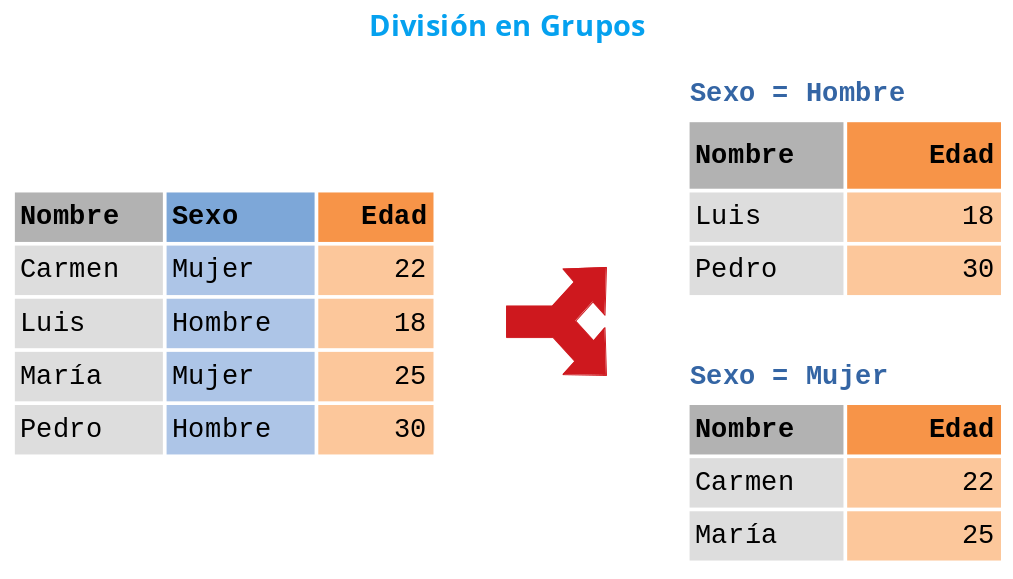
\includegraphics[keepaspectratio]{img/pandas-grupos.png}}

}

\caption{División en grupos de un DataFrame}

\end{figure}%

\subsection{Dividir un DataFrame en
grupos}\label{dividir-un-dataframe-en-grupos}

Para dividir un DataFrame en grupos se utiliza el siguiente método:

\begin{itemize}
\tightlist
\item
  \texttt{df.groupby(columnas).groups} : Devuelve un diccionario con
  cuyas claves son las tuplas que resultan de todas las combinaciones de
  los valores de las columnas con nombres en la lista \texttt{columnas},
  y valores las listas de los nombres de las filas que contienen esos
  valores en las correspondientes columnas del DataFrame \texttt{df}.
\end{itemize}

\begin{Shaded}
\begin{Highlighting}[]
\OperatorTok{\textgreater{}\textgreater{}\textgreater{}} \ImportTok{import}\NormalTok{ pandas }\ImportTok{as}\NormalTok{ pd}
\OperatorTok{\textgreater{}\textgreater{}\textgreater{}}\NormalTok{ df }\OperatorTok{=}\NormalTok{ pd.read\_csv(}
\StringTok{\textquotesingle{}https://raw.githubusercontent.com/asalber/manual{-}python/master/datos/colesterol.csv\textquotesingle{}}\NormalTok{)}
\OperatorTok{\textgreater{}\textgreater{}\textgreater{}} \BuiltInTok{print}\NormalTok{(df.groupby(}\StringTok{\textquotesingle{}sexo\textquotesingle{}}\NormalTok{).groups)}
\NormalTok{\{}\StringTok{\textquotesingle{}H\textquotesingle{}}\NormalTok{: Int64Index([}\DecValTok{0}\NormalTok{, }\DecValTok{2}\NormalTok{, }\DecValTok{5}\NormalTok{, }\DecValTok{6}\NormalTok{, }\DecValTok{8}\NormalTok{, }\DecValTok{9}\NormalTok{, }\DecValTok{11}\NormalTok{, }\DecValTok{12}\NormalTok{], dtype}\OperatorTok{=}\StringTok{\textquotesingle{}int64\textquotesingle{}}\NormalTok{), }\StringTok{\textquotesingle{}M\textquotesingle{}}\NormalTok{: Int64Index([}\DecValTok{1}\NormalTok{, }\DecValTok{3}\NormalTok{, }\DecValTok{4}\NormalTok{, }\DecValTok{7}\NormalTok{, }\DecValTok{10}\NormalTok{, }\DecValTok{13}\NormalTok{], dtype}\OperatorTok{=}\StringTok{\textquotesingle{}int64\textquotesingle{}}\NormalTok{)\}}
\OperatorTok{\textgreater{}\textgreater{}\textgreater{}} \BuiltInTok{print}\NormalTok{(df.groupby([}\StringTok{\textquotesingle{}sexo\textquotesingle{}}\NormalTok{,}\StringTok{\textquotesingle{}edad\textquotesingle{}}\NormalTok{]).groups)}
\NormalTok{\{(}\StringTok{\textquotesingle{}H\textquotesingle{}}\NormalTok{, }\DecValTok{18}\NormalTok{): Int64Index([}\DecValTok{0}\NormalTok{], dtype}\OperatorTok{=}\StringTok{\textquotesingle{}int64\textquotesingle{}}\NormalTok{), (}\StringTok{\textquotesingle{}H\textquotesingle{}}\NormalTok{, }\DecValTok{24}\NormalTok{): Int64Index([}\DecValTok{2}\NormalTok{], dtype}\OperatorTok{=}\StringTok{\textquotesingle{}int64\textquotesingle{}}\NormalTok{), (}\StringTok{\textquotesingle{}H\textquotesingle{}}\NormalTok{, }\DecValTok{27}\NormalTok{): Int64Index([}\DecValTok{12}\NormalTok{], dtype}\OperatorTok{=}\StringTok{\textquotesingle{}int64\textquotesingle{}}\NormalTok{), (}\StringTok{\textquotesingle{}H\textquotesingle{}}\NormalTok{, }\DecValTok{35}\NormalTok{): Int64Index([}\DecValTok{8}\NormalTok{], dtype}\OperatorTok{=}\StringTok{\textquotesingle{}int64\textquotesingle{}}\NormalTok{), (}\StringTok{\textquotesingle{}H\textquotesingle{}}\NormalTok{, }\DecValTok{46}\NormalTok{): Int64Index([}\DecValTok{9}\NormalTok{], dtype}\OperatorTok{=}\StringTok{\textquotesingle{}int64\textquotesingle{}}\NormalTok{), (}\StringTok{\textquotesingle{}H\textquotesingle{}}\NormalTok{, }\DecValTok{51}\NormalTok{): Int64Index([}\DecValTok{6}\NormalTok{], dtype}\OperatorTok{=}\StringTok{\textquotesingle{}int64\textquotesingle{}}\NormalTok{), (}\StringTok{\textquotesingle{}H\textquotesingle{}}\NormalTok{, }\DecValTok{58}\NormalTok{): Int64Index([}\DecValTok{11}\NormalTok{], dtype}\OperatorTok{=}\StringTok{\textquotesingle{}int64\textquotesingle{}}\NormalTok{), (}\StringTok{\textquotesingle{}H\textquotesingle{}}\NormalTok{, }\DecValTok{68}\NormalTok{): Int64Index([}\DecValTok{5}\NormalTok{], dtype}\OperatorTok{=}\StringTok{\textquotesingle{}int64\textquotesingle{}}\NormalTok{), (}\StringTok{\textquotesingle{}M\textquotesingle{}}\NormalTok{, }\DecValTok{20}\NormalTok{): Int64Index([}\DecValTok{13}\NormalTok{], dtype}\OperatorTok{=}\StringTok{\textquotesingle{}int64\textquotesingle{}}\NormalTok{), (}\StringTok{\textquotesingle{}M\textquotesingle{}}\NormalTok{, }\DecValTok{22}\NormalTok{): Int64Index([}\DecValTok{7}\NormalTok{], dtype}\OperatorTok{=}\StringTok{\textquotesingle{}int64\textquotesingle{}}\NormalTok{), (}\StringTok{\textquotesingle{}M\textquotesingle{}}\NormalTok{, }\DecValTok{32}\NormalTok{): Int64Index([}\DecValTok{1}\NormalTok{], dtype}\OperatorTok{=}\StringTok{\textquotesingle{}int64\textquotesingle{}}\NormalTok{), (}\StringTok{\textquotesingle{}M\textquotesingle{}}\NormalTok{, }\DecValTok{35}\NormalTok{): Int64Index([}\DecValTok{3}\NormalTok{], dtype}\OperatorTok{=}\StringTok{\textquotesingle{}int64\textquotesingle{}}\NormalTok{), (}\StringTok{\textquotesingle{}M\textquotesingle{}}\NormalTok{, }\DecValTok{46}\NormalTok{): Int64Index([}\DecValTok{4}\NormalTok{], dtype}\OperatorTok{=}\StringTok{\textquotesingle{}int64\textquotesingle{}}\NormalTok{), (}\StringTok{\textquotesingle{}M\textquotesingle{}}\NormalTok{, }\DecValTok{53}\NormalTok{): Int64Index([}\DecValTok{10}\NormalTok{], dtype}\OperatorTok{=}\StringTok{\textquotesingle{}int64\textquotesingle{}}\NormalTok{)\}}
\end{Highlighting}
\end{Shaded}

Para obtener un grupo concreto se utiliza el siguiente método:

\begin{itemize}
\tightlist
\item
  \texttt{df.groupby(columnas).get\_group(valores)} : Devuelve un
  DataFrame con las filas del DataFrame \texttt{df} que cumplen que las
  columnas de la lista \texttt{columnas} presentan los valores de la
  tupla \texttt{valores}. La lista \texttt{columnas} y la tupla
  \texttt{valores} deben tener el mismo tamaño.
\end{itemize}

\begin{Shaded}
\begin{Highlighting}[]
\OperatorTok{\textgreater{}\textgreater{}\textgreater{}} \ImportTok{import}\NormalTok{ pandas }\ImportTok{as}\NormalTok{ pd}
\OperatorTok{\textgreater{}\textgreater{}\textgreater{}}\NormalTok{ df }\OperatorTok{=}\NormalTok{ pd.read\_csv(}
\StringTok{\textquotesingle{}https://raw.githubusercontent.com/asalber/manual{-}python/master/datos/colesterol.csv\textquotesingle{}}\NormalTok{)}
\OperatorTok{\textgreater{}\textgreater{}\textgreater{}} \BuiltInTok{print}\NormalTok{(df.groupby(}\StringTok{\textquotesingle{}sexo\textquotesingle{}}\NormalTok{).get\_group(}\StringTok{\textquotesingle{}M\textquotesingle{}}\NormalTok{))}
\NormalTok{                    nombre  edad sexo    peso   altura    colesterol}
\DecValTok{1}\NormalTok{           Rosa Díaz Díaz    }\DecValTok{32}\NormalTok{    M    }\FloatTok{65.0}     \FloatTok{1.73}         \FloatTok{232.0}
\DecValTok{3}\NormalTok{      Carmen López Pinzón    }\DecValTok{35}\NormalTok{    M    }\FloatTok{65.0}     \FloatTok{1.70}         \FloatTok{200.0}
\DecValTok{4}\NormalTok{     Marisa López Collado    }\DecValTok{46}\NormalTok{    M    }\FloatTok{51.0}     \FloatTok{1.58}         \FloatTok{148.0}
\DecValTok{7}\NormalTok{    Pilar Martín González    }\DecValTok{22}\NormalTok{    M    }\FloatTok{60.0}     \FloatTok{1.66}\NormalTok{           NaN}
\DecValTok{10}\NormalTok{   Macarena Álvarez Luna    }\DecValTok{53}\NormalTok{    M    }\FloatTok{55.0}     \FloatTok{1.62}         \FloatTok{262.0}
\DecValTok{13}\NormalTok{   Carolina Rubio Moreno    }\DecValTok{20}\NormalTok{    M    }\FloatTok{61.0}     \FloatTok{1.77}         \FloatTok{194.0}
\end{Highlighting}
\end{Shaded}

\subsection{Aplicar una función de agregación por
grupos}\label{aplicar-una-funciuxf3n-de-agregaciuxf3n-por-grupos}

Una vez dividido el DataFame en grupos, es posible aplicar funciones de
agregación a cada grupo mediante el siguiente método:

\begin{itemize}
\tightlist
\item
  \texttt{df.groupby(columnas).agg(funciones)} : Devuelve un DataFrame
  con el resultado de aplicar las funciones de agregación de la lista
  \texttt{funciones} a cada uno de los DataFrames que resultan de
  dividir el DataFrame según las columnas de la lista \texttt{columnas}.
\end{itemize}

Una función de agregación toma como argumento una lista y devuelve una
único valor. Algunas de las funciones de agregación más comunes son:

\begin{itemize}
\tightlist
\item
  \texttt{np.min} : Devuelve el mínimo de una lista de valores.
\item
  \texttt{np.max} : Devuelve el máximo de una lista de valores.
\item
  \texttt{np.count\_nonzero} : Devuelve el número de valores no nulos de
  una lista de valores.
\item
  \texttt{np.sum} : Devuelve la suma de una lista de valores.
\item
  \texttt{np.mean} : Devuelve la media de una lista de valores.
\item
  \texttt{np.std} : Devuelve la desviación típica de una lista de
  valores.
\end{itemize}

\begin{Shaded}
\begin{Highlighting}[]
\OperatorTok{\textgreater{}\textgreater{}\textgreater{}} \ImportTok{import}\NormalTok{ pandas }\ImportTok{as}\NormalTok{ pd}
\OperatorTok{\textgreater{}\textgreater{}\textgreater{}}\NormalTok{ df }\OperatorTok{=}\NormalTok{ pd.read\_csv(}
\StringTok{\textquotesingle{}https://raw.githubusercontent.com/asalber/manual{-}python/master/datos/colesterol.csv\textquotesingle{}}\NormalTok{)}
\OperatorTok{\textgreater{}\textgreater{}\textgreater{}} \BuiltInTok{print}\NormalTok{(df.groupby(}\StringTok{\textquotesingle{}sexo\textquotesingle{}}\NormalTok{).agg(np.mean))}
\NormalTok{           edad       peso    altura  colesterol}
\NormalTok{sexo                                            }
\NormalTok{H     }\FloatTok{40.875000}  \FloatTok{80.714286}  \FloatTok{1.837500}     \FloatTok{228.375}
\NormalTok{M     }\FloatTok{34.666667}  \FloatTok{59.500000}  \FloatTok{1.676667}     \FloatTok{207.200}
\end{Highlighting}
\end{Shaded}

\section{Reestructurar un DataFrame}\label{reestructurar-un-dataframe}

A menudo la disposición de los datos en un DataFrame no es la adecuada
para su tratamiento y es necesario reestructurar el DataFrame. Los datos
que contiene un DataFrame pueden organizarse en dos formatos: ancho y
largo.

\begin{figure}[H]

{\centering \pandocbounded{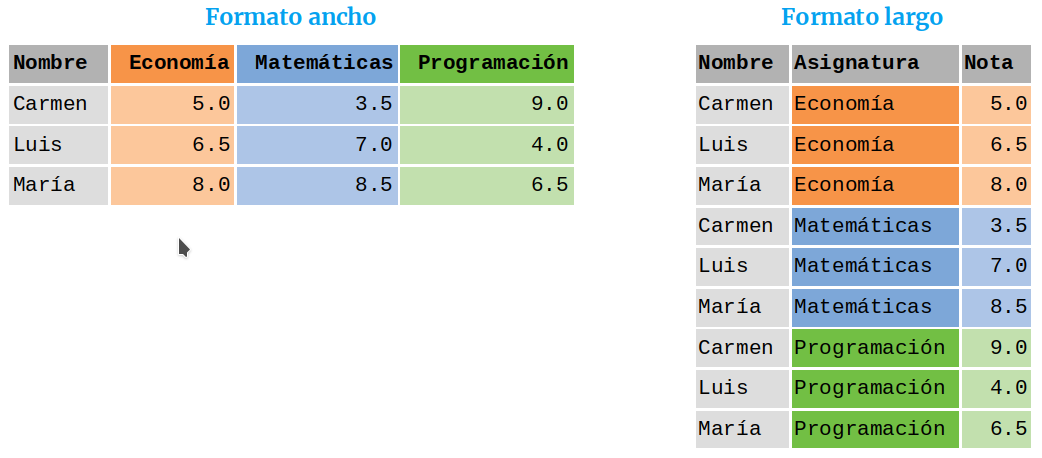
\includegraphics[keepaspectratio]{img/formatos-dataframe.png}}

}

\caption{Formatos de un DataFrame}

\end{figure}%

\subsection{Convertir un DataFrame a formato
largo}\label{convertir-un-dataframe-a-formato-largo}

Para convertir un DataFrame de formato ancho a formato largo (columnas a
filas) se utiliza el siguiente método:

\begin{itemize}
\tightlist
\item
  \texttt{df.melt(id\_vars=id-columnas,\ value\_vars=columnas,\ var\_name=nombre-columnas,\ var\_value=nombre-valores)}
  : Devuelve el DataFrame que resulta de convertir el DataFrame
  \texttt{df} de formato ancho a formato largo. Todas las columnas de
  lista \texttt{columnas} se reestructuran en dos nuevas columnas con
  nombres \texttt{nombre-columnas} y \texttt{nombre-valores} que
  contienen los nombres de las columnas originales y sus valores,
  respectivamente. Las columnas en la lista \texttt{id-columnas} se
  mantienen sin reestructurar. Si no se pasa la lista \texttt{columnas}
  entonces se reestructuran todas las columnas excepto las columnas de
  la lista \texttt{id-columnas}.
\end{itemize}

\begin{Shaded}
\begin{Highlighting}[]
\OperatorTok{\textgreater{}\textgreater{}\textgreater{}} \ImportTok{import}\NormalTok{ pandas }\ImportTok{as}\NormalTok{ pd}
\OperatorTok{\textgreater{}\textgreater{}\textgreater{}}\NormalTok{ datos }\OperatorTok{=}\NormalTok{ \{}\StringTok{\textquotesingle{}nombre\textquotesingle{}}\NormalTok{:[}\StringTok{\textquotesingle{}María\textquotesingle{}}\NormalTok{, }\StringTok{\textquotesingle{}Luis\textquotesingle{}}\NormalTok{, }\StringTok{\textquotesingle{}Carmen\textquotesingle{}}\NormalTok{],}
\NormalTok{... }\StringTok{\textquotesingle{}edad\textquotesingle{}}\NormalTok{:[}\DecValTok{18}\NormalTok{, }\DecValTok{22}\NormalTok{, }\DecValTok{20}\NormalTok{],}
\NormalTok{... }\StringTok{\textquotesingle{}Matemáticas\textquotesingle{}}\NormalTok{:[}\FloatTok{8.5}\NormalTok{, }\DecValTok{7}\NormalTok{, }\FloatTok{3.5}\NormalTok{],}
\NormalTok{... }\StringTok{\textquotesingle{}Economía\textquotesingle{}}\NormalTok{:[}\DecValTok{8}\NormalTok{, }\FloatTok{6.5}\NormalTok{, }\DecValTok{5}\NormalTok{],}
\NormalTok{... }\StringTok{\textquotesingle{}Programación\textquotesingle{}}\NormalTok{:[}\FloatTok{6.5}\NormalTok{, }\DecValTok{4}\NormalTok{, }\DecValTok{9}\NormalTok{]\}}
\OperatorTok{\textgreater{}\textgreater{}\textgreater{}}\NormalTok{ df }\OperatorTok{=}\NormalTok{ pd.DataFrame(datos)}
\OperatorTok{\textgreater{}\textgreater{}\textgreater{}}\NormalTok{ df1 }\OperatorTok{=}\NormalTok{ df.melt(id\_vars}\OperatorTok{=}\NormalTok{[}\StringTok{\textquotesingle{}nombre\textquotesingle{}}\NormalTok{, }\StringTok{\textquotesingle{}edad\textquotesingle{}}\NormalTok{], var\_name}\OperatorTok{=}\StringTok{\textquotesingle{}asignatura\textquotesingle{}}\NormalTok{, value\_name}\OperatorTok{=}\StringTok{\textquotesingle{}nota\textquotesingle{}}\NormalTok{)}
\OperatorTok{\textgreater{}\textgreater{}\textgreater{}} \BuiltInTok{print}\NormalTok{(df1)}
\NormalTok{   nombre  edad    asignatura  nota}
\DecValTok{0}\NormalTok{   María    }\DecValTok{18}\NormalTok{   Matemáticas   }\FloatTok{8.5}
\DecValTok{1}\NormalTok{    Luis    }\DecValTok{22}\NormalTok{   Matemáticas   }\FloatTok{7.0}
\DecValTok{2}\NormalTok{  Carmen    }\DecValTok{20}\NormalTok{   Matemáticas   }\FloatTok{3.5}
\DecValTok{3}\NormalTok{   María    }\DecValTok{18}\NormalTok{      Economía   }\FloatTok{8.0}
\DecValTok{4}\NormalTok{    Luis    }\DecValTok{22}\NormalTok{      Economía   }\FloatTok{6.5}
\DecValTok{5}\NormalTok{  Carmen    }\DecValTok{20}\NormalTok{      Economía   }\FloatTok{5.0}
\DecValTok{6}\NormalTok{   María    }\DecValTok{18}\NormalTok{  Programación   }\FloatTok{6.5}
\DecValTok{7}\NormalTok{    Luis    }\DecValTok{22}\NormalTok{  Programación   }\FloatTok{4.0}
\DecValTok{8}\NormalTok{  Carmen    }\DecValTok{20}\NormalTok{  Programación   }\FloatTok{9.0}
\end{Highlighting}
\end{Shaded}

\subsection{Convertir un DataFrame a formato
ancho}\label{convertir-un-dataframe-a-formato-ancho}

Para convertir un DataFrame de formato largo a formato ancho (filas a
columnas) se utiliza el siguiente método:

\begin{itemize}
\tightlist
\item
  \texttt{df.pivot(index=filas,\ columns=columna,\ values=valores)} :
  Devuelve el DataFrame que resulta de convertir el DataFrame
  \texttt{df} de formato largo a formato ancho. Se crean tantas columnas
  nuevas como valores distintos haya en la columna \texttt{columna}. Los
  nombres de estas nuevas columnas son los valores de la columna
  \texttt{columna} mientras que sus valores se toman de la columna
  \texttt{valores}. Los nombres del índice del nuevo DataFrame se toman
  de los valores de la columna \texttt{filas}.
\end{itemize}

\begin{Shaded}
\begin{Highlighting}[]
\CommentTok{\# Continuación del código anterior}
\OperatorTok{\textgreater{}\textgreater{}\textgreater{}} \BuiltInTok{print}\NormalTok{(df1.pivot(index}\OperatorTok{=}\StringTok{\textquotesingle{}nombre\textquotesingle{}}\NormalTok{, columns}\OperatorTok{=}\StringTok{\textquotesingle{}asignatura\textquotesingle{}}\NormalTok{, values}\OperatorTok{=}\StringTok{\textquotesingle{}nota\textquotesingle{}}\NormalTok{))}
\NormalTok{asignatura  Economía  Matemáticas  Programación}
\NormalTok{nombre                                  }
\NormalTok{Carmen           }\FloatTok{5.0}          \FloatTok{3.5}           \FloatTok{9.0}
\NormalTok{Luis             }\FloatTok{6.5}          \FloatTok{7.0}           \FloatTok{4.0}
\NormalTok{María            }\FloatTok{8.0}          \FloatTok{8.5}           \FloatTok{6.5}
\end{Highlighting}
\end{Shaded}

\section{Combinar varios DataFrames}\label{combinar-varios-dataframes}

Dos o más DataFrames pueden combinarse en otro DataFrame. La combinación
puede ser de varias formas:

\begin{itemize}
\tightlist
\item
  \textbf{Concatenación}: Combinación de varios DataFrames concatenando
  sus filas o columnas.
\item
  \textbf{Mezcla}: Combinación de varios DataFrames usando columnas o
  índices comunes.
\end{itemize}

\subsection{Concatenación de
DataFrames}\label{concatenaciuxf3n-de-dataframes}

\begin{itemize}
\item
  \textbf{Concatenación de filas}. Las filas de los DataFrames se
  concatenan unas a continuación de las otras para formar el nuevo
  DataFrame. Para ello es necesario que los DataFrames que se combinen
  tengan el mismo índice de columnas.

  \begin{figure}[H]

  {\centering \pandocbounded{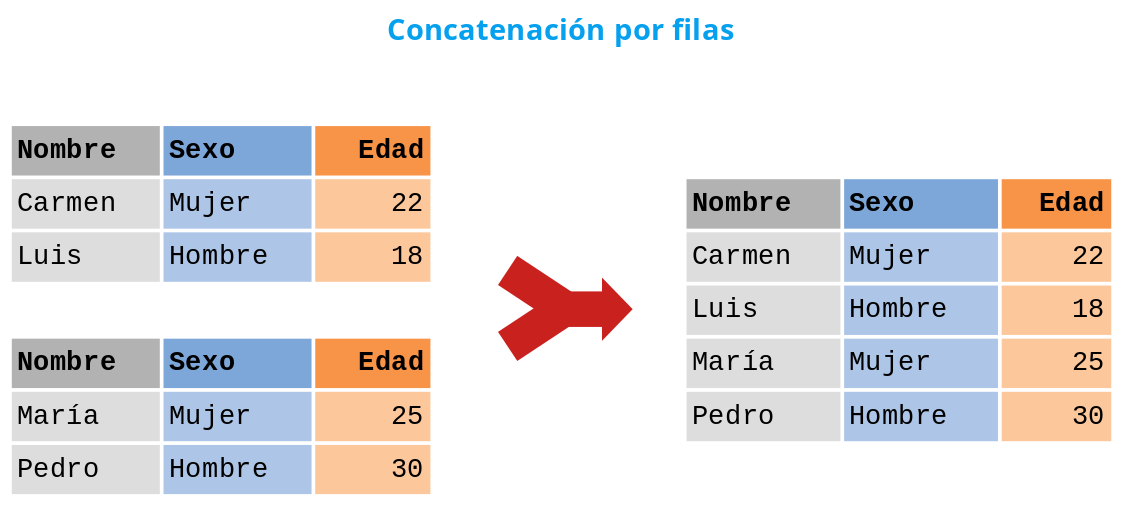
\includegraphics[keepaspectratio]{img/pandas-concatenacion-filas.png}}

  }

  \caption{Concatenación de DataFrames por filas}

  \end{figure}%
\item
  \textbf{Concatenación de columnas}. Las columnas de los DataFrames se
  concatenan unas a continuación de las otras para formar el nuevo
  DataFrame. Para ello es necesario que los DataFrames que se combinen
  tengan el mismo índice de filas.

  \begin{figure}[H]

  {\centering \pandocbounded{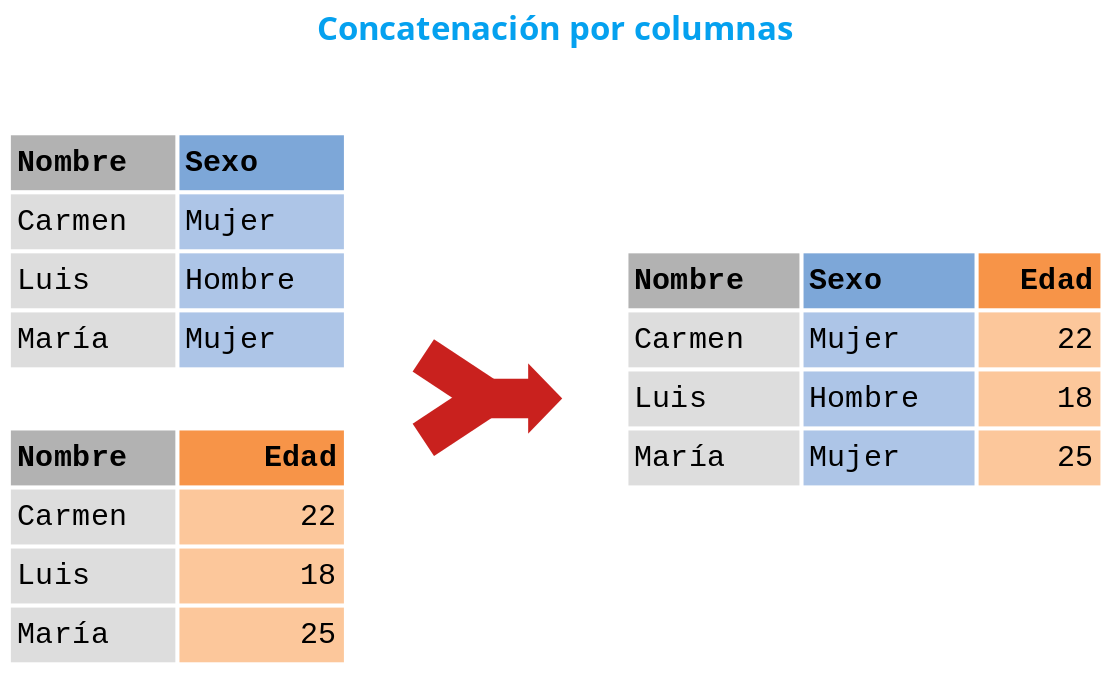
\includegraphics[keepaspectratio]{img/pandas-concatenacion-columnas.png}}

  }

  \caption{Concatenación de DataFrames por columnas}

  \end{figure}%
\end{itemize}

Para concatenar dos o más DataFrames se utiliza el siguiente método:

\begin{itemize}
\tightlist
\item
  \texttt{df.concat(dataframes,\ axis\ =\ eje)}: Devuelve el DataFrame
  que resulta de concatenar los DataFrames de la lista
  \texttt{dataframes}. Si \texttt{eje} es 0 (valor por defecto) la
  concatenación se realiza por filas, y si \texttt{eje} es 1 se realiza
  por columnas.
\end{itemize}

\begin{tcolorbox}[enhanced jigsaw, arc=.35mm, bottomrule=.15mm, bottomtitle=1mm, breakable, colback=white, colbacktitle=quarto-callout-warning-color!10!white, colframe=quarto-callout-warning-color-frame, coltitle=black, left=2mm, leftrule=.75mm, opacityback=0, opacitybacktitle=0.6, rightrule=.15mm, title=\textcolor{quarto-callout-warning-color}{\faExclamationTriangle}\hspace{0.5em}{Advertencia}, titlerule=0mm, toprule=.15mm, toptitle=1mm]

Si los DataFrames que se concatenan por filas no tienen el mismo índice
de columnas, el DataFrame resultante incluirá todas las columnas
existentes en los DataFrames y rellenará con valores \texttt{NaN} los
datos no disponibles. Si los DataFrames que se concatenan por columnas
no tienen el mismo índice de filas, el DataFrame resultante incluirá
todas las filas existentes en los DataFrames y rellenará con valores
\texttt{NaN} los datos no disponibles.

\end{tcolorbox}

\begin{Shaded}
\begin{Highlighting}[]
\OperatorTok{\textgreater{}\textgreater{}\textgreater{}} \ImportTok{import}\NormalTok{ pandas }\ImportTok{as}\NormalTok{ pd}
\OperatorTok{\textgreater{}\textgreater{}\textgreater{}}\NormalTok{ df1 }\OperatorTok{=}\NormalTok{ pd.DataFrame(\{}\StringTok{"Nombre"}\NormalTok{:[}\StringTok{"Carmen"}\NormalTok{, }\StringTok{"Luis"}\NormalTok{], }
\NormalTok{... }\StringTok{"Sexo"}\NormalTok{:[}\StringTok{"Mujer"}\NormalTok{, }\StringTok{"Hombre"}\NormalTok{], }\StringTok{"Edad"}\NormalTok{:[}\DecValTok{22}\NormalTok{, }\DecValTok{18}\NormalTok{]\}).set\_index(}\StringTok{"Nombre"}\NormalTok{)}
\OperatorTok{\textgreater{}\textgreater{}\textgreater{}}\NormalTok{ df2 }\OperatorTok{=}\NormalTok{ pd.DataFrame(\{}\StringTok{"Nombre"}\NormalTok{:[}\StringTok{"María"}\NormalTok{, }\StringTok{"Pedro"}\NormalTok{], }
\NormalTok{... }\StringTok{"Sexo"}\NormalTok{:[}\StringTok{"Mujer"}\NormalTok{, }\StringTok{"Hombre"}\NormalTok{], }\StringTok{"Edad"}\NormalTok{:[}\DecValTok{25}\NormalTok{, }\DecValTok{30}\NormalTok{]\}).set\_index(}\StringTok{"Nombre"}\NormalTok{)}
\OperatorTok{\textgreater{}\textgreater{}\textgreater{}}\NormalTok{ df }\OperatorTok{=}\NormalTok{ pd.concat([df1, df2])}
\OperatorTok{\textgreater{}\textgreater{}\textgreater{}}\NormalTok{ df}
\NormalTok{          Sexo  Edad}
\NormalTok{Nombre              }
\NormalTok{Carmen   Mujer    }\DecValTok{22}
\NormalTok{Luis    Hombre    }\DecValTok{18}
\NormalTok{María    Mujer    }\DecValTok{25}
\NormalTok{Pedro   Hombre    }\DecValTok{30}
\end{Highlighting}
\end{Shaded}

\begin{Shaded}
\begin{Highlighting}[]
\OperatorTok{\textgreater{}\textgreater{}\textgreater{}} \ImportTok{import}\NormalTok{ pandas }\ImportTok{as}\NormalTok{ pd}
\OperatorTok{\textgreater{}\textgreater{}\textgreater{}}\NormalTok{ df1 }\OperatorTok{=}\NormalTok{ pd.DataFrame(\{}\StringTok{"Nombre"}\NormalTok{:[}\StringTok{"Carmen"}\NormalTok{, }\StringTok{"Luis"}\NormalTok{, }\StringTok{"María"}\NormalTok{], }
\NormalTok{... }\StringTok{"Sexo"}\NormalTok{:[}\StringTok{"Mujer"}\NormalTok{, }\StringTok{"Hombre"}\NormalTok{, }\StringTok{"Mujer"}\NormalTok{]\}).set\_index(}\StringTok{"Nombre"}\NormalTok{)}
\OperatorTok{\textgreater{}\textgreater{}\textgreater{}}\NormalTok{ df2 }\OperatorTok{=}\NormalTok{ pd.DataFrame(\{}\StringTok{"Nombre"}\NormalTok{:[}\StringTok{"Carmen"}\NormalTok{, }\StringTok{"Luis"}\NormalTok{, }\StringTok{"María"}\NormalTok{], }
\NormalTok{... }\StringTok{"Edad"}\NormalTok{:[}\DecValTok{22}\NormalTok{, }\DecValTok{18}\NormalTok{, }\DecValTok{25}\NormalTok{]\}).set\_index(}\StringTok{"Nombre"}\NormalTok{)}
\OperatorTok{\textgreater{}\textgreater{}\textgreater{}}\NormalTok{ df }\OperatorTok{=}\NormalTok{ pd.concat([df1, df2], axis }\OperatorTok{=} \DecValTok{1}\NormalTok{)}
\OperatorTok{\textgreater{}\textgreater{}\textgreater{}}\NormalTok{ df}
\NormalTok{          Sexo  Edad}
\NormalTok{Nombre              }
\NormalTok{Carmen   Mujer    }\DecValTok{22}
\NormalTok{Luis    Hombre    }\DecValTok{18}
\NormalTok{María    Mujer    }\DecValTok{25}
\end{Highlighting}
\end{Shaded}

\subsection{Mezcla de DataFrames}\label{mezcla-de-dataframes}

La mezcla de DataFrames permite integrar filas de dos DataFrames que
contienen información en común en una o varias columnas o índices que se
conocen como \emph{clave}.

Para mezclar dos DataFrames se utiliza el siguiente método:

\begin{itemize}
\tightlist
\item
  \texttt{df.merge(df1,\ df2,\ on\ =\ clave,\ how\ =\ tipo)}: Devuelve
  el DataFrame que resulta de mezclar el DataFrame \texttt{df2} con el
  DataFrame \texttt{df1}, usando como claves las columnas de la lista
  \texttt{clave} y siguiendo el método de mezcla indicado por
  \texttt{tipo}.
\end{itemize}

El tipo de mezcla puede ser

\begin{itemize}
\item
  \texttt{"inner"} (por defecto): El DataFrame resultante solo contiene
  las filas cuyos valores en la clave están en los dos DataFrames. Es
  equivalente a la intersección de conjuntos.

\begin{Shaded}
\begin{Highlighting}[]
\OperatorTok{\textgreater{}\textgreater{}\textgreater{}} \ImportTok{import}\NormalTok{ pandas }\ImportTok{as}\NormalTok{ pd}
\OperatorTok{\textgreater{}\textgreater{}\textgreater{}}\NormalTok{ df1 }\OperatorTok{=}\NormalTok{ pd.DataFrame(\{}\StringTok{"Nombre"}\NormalTok{:[}\StringTok{"Carmen"}\NormalTok{, }\StringTok{"Luis"}\NormalTok{, }\StringTok{"María"}\NormalTok{],  }\StringTok{"Sexo"}\NormalTok{:[}\StringTok{"Mujer"}\NormalTok{, }\StringTok{"Hombre"}\NormalTok{, }\StringTok{"Mujer"}\NormalTok{]\})}
\OperatorTok{\textgreater{}\textgreater{}\textgreater{}}\NormalTok{ df2 }\OperatorTok{=}\NormalTok{ pd.DataFrame(\{}\StringTok{"Nombre"}\NormalTok{:[}\StringTok{"María"}\NormalTok{, }\StringTok{"Pedro"}\NormalTok{, }\StringTok{"Luis"}\NormalTok{], }\StringTok{"Edad"}\NormalTok{:[}\DecValTok{25}\NormalTok{, }\DecValTok{30}\NormalTok{, }\DecValTok{18}\NormalTok{]]\})}
\OperatorTok{\textgreater{}\textgreater{}\textgreater{}}\NormalTok{ df }\OperatorTok{=}\NormalTok{ pd.merge(df1, df2, on}\OperatorTok{=}\StringTok{"Nombre"}\NormalTok{)}
\OperatorTok{\textgreater{}\textgreater{}\textgreater{}} \BuiltInTok{print}\NormalTok{(df)}
\NormalTok{  Nombre    Sexo  Edad}
\DecValTok{0}\NormalTok{   Luis  Hombre    }\DecValTok{18}
\DecValTok{1}\NormalTok{  María   Mujer    }\DecValTok{25}
\end{Highlighting}
\end{Shaded}
\item
  \texttt{"outer"}: El DataFrame resultante contiene todas las filas de
  los dos DataFrames. Si una fila de un DataFrame no puede emparejarse
  con otra los mismos valores en la clave en el otro DataFrame, la fila
  se añade igualmente al DataFrame resultante rellenando las columnas
  del otro DataFrame con el valor \texttt{NaN}. Es equivalente a la
  unión de conjuntos.

\begin{Shaded}
\begin{Highlighting}[]
\OperatorTok{\textgreater{}\textgreater{}\textgreater{}} \ImportTok{import}\NormalTok{ pandas }\ImportTok{as}\NormalTok{ pd}
\OperatorTok{\textgreater{}\textgreater{}\textgreater{}}\NormalTok{ df1 }\OperatorTok{=}\NormalTok{ pd.DataFrame(\{}\StringTok{"Nombre"}\NormalTok{:[}\StringTok{"Carmen"}\NormalTok{, }\StringTok{"Luis"}\NormalTok{, }\StringTok{"María"}\NormalTok{],  }\StringTok{"Sexo"}\NormalTok{:[}\StringTok{"Mujer"}\NormalTok{, }\StringTok{"Hombre"}\NormalTok{, }\StringTok{"Mujer"}\NormalTok{]\})}
\OperatorTok{\textgreater{}\textgreater{}\textgreater{}}\NormalTok{ df2 }\OperatorTok{=}\NormalTok{ pd.DataFrame(\{}\StringTok{"Nombre"}\NormalTok{:[}\StringTok{"María"}\NormalTok{, }\StringTok{"Pedro"}\NormalTok{, }\StringTok{"Luis"}\NormalTok{], }\StringTok{"Edad"}\NormalTok{:[}\DecValTok{25}\NormalTok{, }\DecValTok{30}\NormalTok{, }\DecValTok{18}\NormalTok{]]\})}
\OperatorTok{\textgreater{}\textgreater{}\textgreater{}}\NormalTok{ df }\OperatorTok{=}\NormalTok{ pd.merge(df1, df2, on}\OperatorTok{=}\StringTok{"Nombre"}\NormalTok{, how}\OperatorTok{=}\StringTok{"outer"}\NormalTok{)}
\OperatorTok{\textgreater{}\textgreater{}\textgreater{}} \BuiltInTok{print}\NormalTok{(df)}
\NormalTok{   Nombre    Sexo  Edad}
\DecValTok{0}\NormalTok{  Carmen   Mujer   NaN}
\DecValTok{1}\NormalTok{    Luis  Hombre  }\FloatTok{18.0}
\DecValTok{2}\NormalTok{   María   Mujer  }\FloatTok{25.0}
\DecValTok{3}\NormalTok{   Pedro     NaN  }\FloatTok{30.0}
\end{Highlighting}
\end{Shaded}
\item
  \texttt{"left"}: El DataFrame resultante contiene todas las filas del
  primer DataFrame y descarta las filas del segundo DataFrame que no
  pueden emparejarse con alguna fila del primer DataFrame a través de la
  clave.

\begin{Shaded}
\begin{Highlighting}[]
\OperatorTok{\textgreater{}\textgreater{}\textgreater{}} \ImportTok{import}\NormalTok{ pandas }\ImportTok{as}\NormalTok{ pd}
\OperatorTok{\textgreater{}\textgreater{}\textgreater{}}\NormalTok{ df1 }\OperatorTok{=}\NormalTok{ pd.DataFrame(\{}\StringTok{"Nombre"}\NormalTok{:[}\StringTok{"Carmen"}\NormalTok{, }\StringTok{"Luis"}\NormalTok{, }\StringTok{"María"}\NormalTok{],  }\StringTok{"Sexo"}\NormalTok{:[}\StringTok{"Mujer"}\NormalTok{, }\StringTok{"Hombre"}\NormalTok{, }\StringTok{"Mujer"}\NormalTok{]\})}
\OperatorTok{\textgreater{}\textgreater{}\textgreater{}}\NormalTok{ df2 }\OperatorTok{=}\NormalTok{ pd.DataFrame(\{}\StringTok{"Nombre"}\NormalTok{:[}\StringTok{"María"}\NormalTok{, }\StringTok{"Pedro"}\NormalTok{, }\StringTok{"Luis"}\NormalTok{], }\StringTok{"Edad"}\NormalTok{:[}\DecValTok{25}\NormalTok{, }\DecValTok{30}\NormalTok{, }\DecValTok{18}\NormalTok{]]\})}
\OperatorTok{\textgreater{}\textgreater{}\textgreater{}}\NormalTok{ df }\OperatorTok{=}\NormalTok{ pd.merge(df1, df2, on}\OperatorTok{=}\StringTok{"Nombre"}\NormalTok{, how}\OperatorTok{=}\StringTok{"left"}\NormalTok{)}
\OperatorTok{\textgreater{}\textgreater{}\textgreater{}} \BuiltInTok{print}\NormalTok{(df)}
\NormalTok{   Nombre    Sexo  Edad}
\DecValTok{0}\NormalTok{  Carmen   Mujer   NaN}
\DecValTok{1}\NormalTok{    Luis  Hombre  }\FloatTok{18.0}
\DecValTok{2}\NormalTok{   María   Mujer  }\FloatTok{25.0}
\end{Highlighting}
\end{Shaded}
\item
  \texttt{"right"}: El DataFrame resultante contiene todas las filas del
  segundo DataFrame y descarta las filas del primer DataFrame que no
  pueden emparejarse con alguna fila del segundo DataFrame a través de
  la clave.

\begin{Shaded}
\begin{Highlighting}[]
\OperatorTok{\textgreater{}\textgreater{}\textgreater{}} \ImportTok{import}\NormalTok{ pandas }\ImportTok{as}\NormalTok{ pd}
\OperatorTok{\textgreater{}\textgreater{}\textgreater{}}\NormalTok{ df1 }\OperatorTok{=}\NormalTok{ pd.DataFrame(\{}\StringTok{"Nombre"}\NormalTok{:[}\StringTok{"Carmen"}\NormalTok{, }\StringTok{"Luis"}\NormalTok{, }\StringTok{"María"}\NormalTok{],  }\StringTok{"Sexo"}\NormalTok{:[}\StringTok{"Mujer"}\NormalTok{, }\StringTok{"Hombre"}\NormalTok{, }\StringTok{"Mujer"}\NormalTok{]\})}
\OperatorTok{\textgreater{}\textgreater{}\textgreater{}}\NormalTok{ df2 }\OperatorTok{=}\NormalTok{ pd.DataFrame(\{}\StringTok{"Nombre"}\NormalTok{:[}\StringTok{"María"}\NormalTok{, }\StringTok{"Pedro"}\NormalTok{, }\StringTok{"Luis"}\NormalTok{], }\StringTok{"Edad"}\NormalTok{:[}\DecValTok{25}\NormalTok{, }\DecValTok{30}\NormalTok{, }\DecValTok{18}\NormalTok{]]\})}
\OperatorTok{\textgreater{}\textgreater{}\textgreater{}}\NormalTok{ df }\OperatorTok{=}\NormalTok{ pd.merge(df1, df2, on}\OperatorTok{=}\StringTok{"Nombre"}\NormalTok{, how}\OperatorTok{=}\StringTok{"right"}\NormalTok{)}
\OperatorTok{\textgreater{}\textgreater{}\textgreater{}} \BuiltInTok{print}\NormalTok{(df)}
\NormalTok{  Nombre    Sexo  Edad}
\DecValTok{0}\NormalTok{  María   Mujer    }\DecValTok{25}
\DecValTok{1}\NormalTok{  Pedro     NaN    }\DecValTok{30}
\DecValTok{2}\NormalTok{   Luis  Hombre    }\DecValTok{18}
\end{Highlighting}
\end{Shaded}
\end{itemize}

\bookmarksetup{startatroot}

\chapter{La librería Matplotlib}\label{la-libreruxeda-matplotlib}

\href{https://matplotlib.org/}{Matplotlib} es una librería de Python
especializada en la creación de gráficos en dos dimensiones.

\begin{figure}[H]

{\centering \pandocbounded{
\includegraphics[keepaspectratio]{img/matplotlib-logo.png}}

}

\caption{Gráfico con matplotlib}

\end{figure}%

Permite crear y personalizar los tipos de gráficos más comunes, entre
ellos:

\begin{itemize}
\tightlist
\item
  Diagramas de barras
\item
  Histograma
\item
  Diagramas de sectores
\item
  Diagramas de caja y bigotes
\item
  Diagramas de violín
\item
  Diagramas de dispersión o puntos
\item
  Diagramas de lineas
\item
  Diagramas de areas
\item
  Diagramas de contorno
\item
  Mapas de color
\end{itemize}

y combinaciones de todos ellos.

En la siguiente \href{https://matplotlib.org/gallery/index.html}{galería
de gráficos} pueden apreciarse todos los tipos de gráficos que pueden
crearse con esta librería.

\section{Creación de gráficos con
matplotlib}\label{creaciuxf3n-de-gruxe1ficos-con-matplotlib}

Para crear un gráfico con matplotlib es habitual seguir los siguientes
pasos:

\begin{enumerate}
\def\labelenumi{\arabic{enumi}.}
\item
  Importar el módulo \texttt{pyplot}.
\item
  Definir la figura que contendrá el gráfico, que es la region (ventana
  o página) donde se dibujará y los ejes sobre los que se dibujarán los
  datos. Para ello se utiliza la función \texttt{subplots()}.
\item
  Dibujar los datos sobre los ejes. Para ello se utilizan distintas
  funciones dependiendo del tipo de gráfico que se quiera.
\item
  Personalizar el gráfico. Para ello existen multitud de funciones que
  permiten añadir un título, una leyenda, una rejilla, cambiar colores o
  personalizar los ejes.
\item
  Guardar el gráfico. Para ello se utiliza la función
  \texttt{savefig()}.
\item
  Mostrar el gráfico. Para ello se utiliza la función \texttt{show()}.
\end{enumerate}

\begin{Shaded}
\begin{Highlighting}[]
\CommentTok{\# Importar el módulo pyplot con el alias plt}
\ImportTok{import}\NormalTok{ matplotlib.pyplot }\ImportTok{as}\NormalTok{ plt}
\CommentTok{\# Crear la figura y los ejes}
\NormalTok{fig, ax }\OperatorTok{=}\NormalTok{ plt.subplots()}
\CommentTok{\# Dibujar puntos}
\NormalTok{ax.scatter(x }\OperatorTok{=}\NormalTok{ [}\DecValTok{1}\NormalTok{, }\DecValTok{2}\NormalTok{, }\DecValTok{3}\NormalTok{], y }\OperatorTok{=}\NormalTok{ [}\DecValTok{3}\NormalTok{, }\DecValTok{2}\NormalTok{, }\DecValTok{1}\NormalTok{])}
\CommentTok{\# Guardar el gráfico en formato png}
\NormalTok{plt.savefig(}\StringTok{\textquotesingle{}diagrama{-}dispersion.png\textquotesingle{}}\NormalTok{)}
\CommentTok{\# Mostrar el gráfico}
\NormalTok{plt.show()}
\end{Highlighting}
\end{Shaded}

\begin{figure}[H]

{\centering \pandocbounded{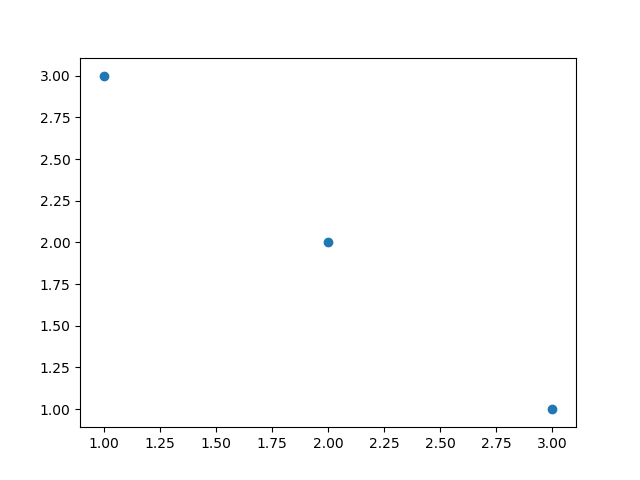
\includegraphics[keepaspectratio]{img/diagrama-dispersion.png}}

}

\caption{Gráfico con matplotlib}

\end{figure}%

\section{Diagramas de dispersión o
puntos}\label{diagramas-de-dispersiuxf3n-o-puntos}

\begin{itemize}
\tightlist
\item
  \texttt{scatter(x,\ y)}: Dibuja un diagrama de puntos con las
  coordenadas de la lista \texttt{x} en el eje X y las coordenadas de la
  lista \texttt{y} en el eje Y.
  \href{https://matplotlib.org/api/_as_gen/matplotlib.pyplot.scatter.html\#matplotlib.pyplot.scatter}{}
\end{itemize}

\begin{Shaded}
\begin{Highlighting}[]
\ImportTok{import}\NormalTok{ matplotlib.pyplot }\ImportTok{as}\NormalTok{ plt}
\NormalTok{fig, ax }\OperatorTok{=}\NormalTok{ plt.subplots()}
\NormalTok{ax.scatter([}\DecValTok{1}\NormalTok{, }\DecValTok{2}\NormalTok{, }\DecValTok{3}\NormalTok{, }\DecValTok{4}\NormalTok{], [}\DecValTok{1}\NormalTok{, }\DecValTok{2}\NormalTok{, }\DecValTok{0}\NormalTok{, }\FloatTok{0.5}\NormalTok{])}
\NormalTok{plt.show()}
\end{Highlighting}
\end{Shaded}

\begin{figure}[H]

{\centering \pandocbounded{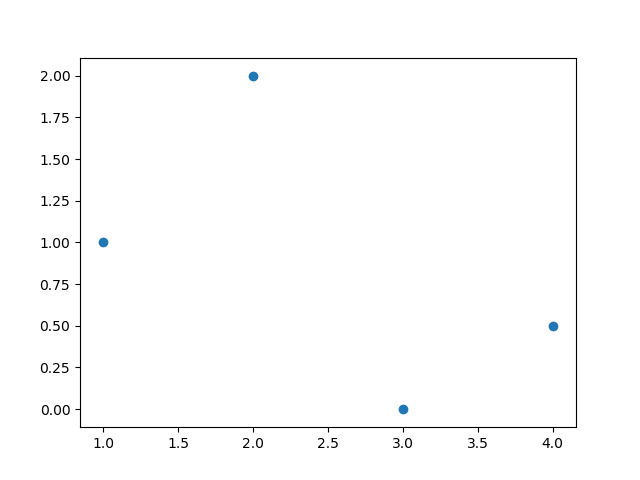
\includegraphics[keepaspectratio]{img/diagrama-puntos.png}}

}

\caption{Gráfico con matplotlib}

\end{figure}%

\section{Diagramas de líneas}\label{diagramas-de-luxedneas}

\begin{itemize}
\tightlist
\item
  \texttt{plot(x,\ y)}: Dibuja un polígono con los vértices dados por
  las coordenadas de la lista \texttt{x} en el eje X y las coordenadas
  de la lista \texttt{y} en el eje Y.
  \href{https://matplotlib.org/api/_as_gen/matplotlib.pyplot.plot.html\#matplotlib.pyplot.plot}{}
\end{itemize}

\begin{Shaded}
\begin{Highlighting}[]
\ImportTok{import}\NormalTok{ matplotlib.pyplot }\ImportTok{as}\NormalTok{ plt}
\NormalTok{fig, ax }\OperatorTok{=}\NormalTok{ plt.subplots()}
\NormalTok{ax.plot([}\DecValTok{1}\NormalTok{, }\DecValTok{2}\NormalTok{, }\DecValTok{3}\NormalTok{, }\DecValTok{4}\NormalTok{], [}\DecValTok{1}\NormalTok{, }\DecValTok{2}\NormalTok{, }\DecValTok{0}\NormalTok{, }\FloatTok{0.5}\NormalTok{])}
\NormalTok{plt.show()}
\end{Highlighting}
\end{Shaded}

\begin{figure}[H]

{\centering \pandocbounded{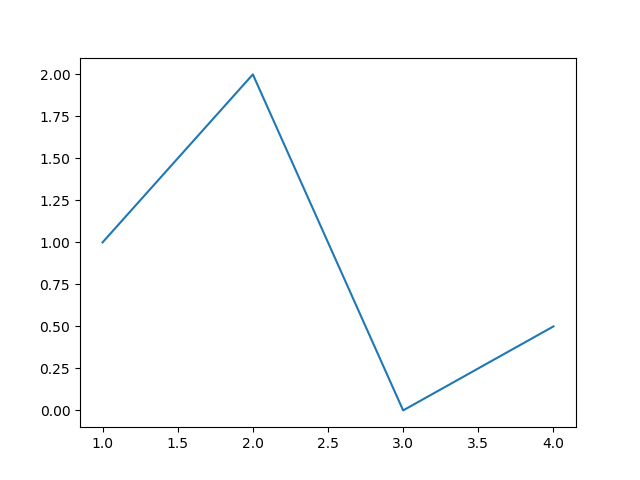
\includegraphics[keepaspectratio]{img/diagrama-lineas.png}}

}

\caption{Gráfico con matplotlib}

\end{figure}%

\section{Diagramas de areas}\label{diagramas-de-areas}

\begin{itemize}
\tightlist
\item
  \texttt{fill\_between(x,\ y)}: Dibuja el area bajo el polígono con los
  vértices dados por las coordenadas de la lista \texttt{x} en el eje X
  y las coordenadas de la lista \texttt{y} en el eje Y.
  \href{https://matplotlib.org/api/_as_gen/matplotlib.pyplot.fill_between.html\#matplotlib.pyplot.fill_between}{}
\end{itemize}

\begin{Shaded}
\begin{Highlighting}[]
\ImportTok{import}\NormalTok{ matplotlib.pyplot }\ImportTok{as}\NormalTok{ plt}
\NormalTok{fig, ax }\OperatorTok{=}\NormalTok{ plt.subplots()}
\NormalTok{ax.fill\_between([}\DecValTok{1}\NormalTok{, }\DecValTok{2}\NormalTok{, }\DecValTok{3}\NormalTok{, }\DecValTok{4}\NormalTok{], [}\DecValTok{1}\NormalTok{, }\DecValTok{2}\NormalTok{, }\DecValTok{0}\NormalTok{, }\FloatTok{0.5}\NormalTok{])}
\NormalTok{plt.show()}
\end{Highlighting}
\end{Shaded}

\begin{figure}[H]

{\centering \pandocbounded{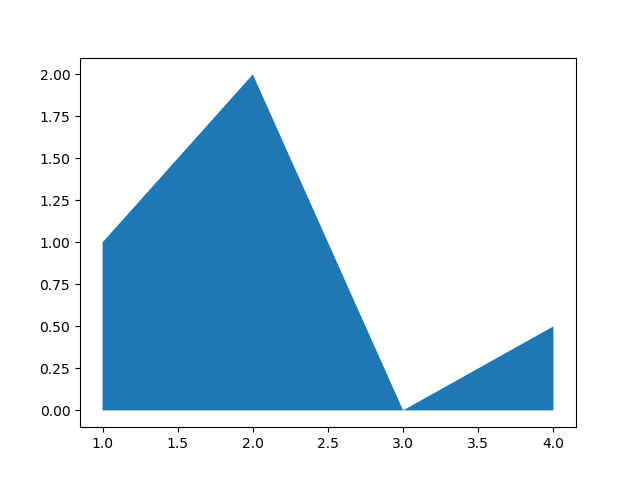
\includegraphics[keepaspectratio]{img/diagrama-areas.png}}

}

\caption{Gráfico con matplotlib}

\end{figure}%

\section{Diagramas de barras
verticales}\label{diagramas-de-barras-verticales}

\begin{itemize}
\tightlist
\item
  \texttt{bar(x,\ y)}: Dibuja un diagrama de barras verticales donde
  \texttt{x} es una lista con la posición de las barras en el eje X, e
  \texttt{y} es una lista con la altura de las barras en el eje Y.
  \href{https://matplotlib.org/api/_as_gen/matplotlib.pyplot.bar.html\#matplotlib.pyplot.bar}{}
\end{itemize}

\begin{Shaded}
\begin{Highlighting}[]
\ImportTok{import}\NormalTok{ matplotlib.pyplot }\ImportTok{as}\NormalTok{ plt}
\NormalTok{fig, ax }\OperatorTok{=}\NormalTok{ plt.subplots()}
\NormalTok{ax.bar([}\DecValTok{1}\NormalTok{, }\DecValTok{2}\NormalTok{, }\DecValTok{3}\NormalTok{], [}\DecValTok{3}\NormalTok{, }\DecValTok{2}\NormalTok{, }\DecValTok{1}\NormalTok{])}
\NormalTok{plt.show()}
\end{Highlighting}
\end{Shaded}

\begin{figure}[H]

{\centering \pandocbounded{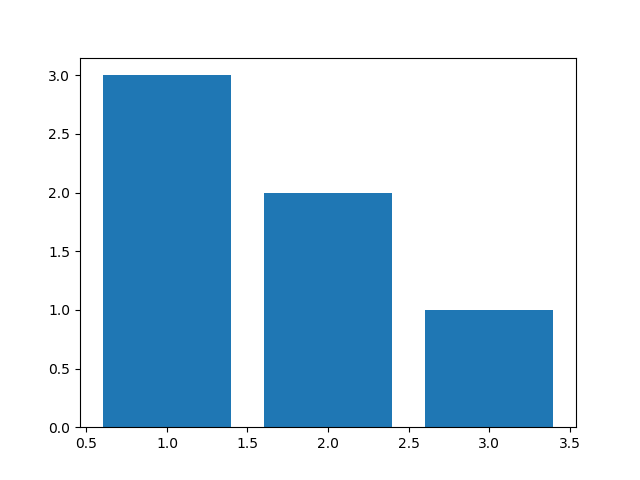
\includegraphics[keepaspectratio]{img/diagrama-barras.png}}

}

\caption{Gráfico con matplotlib}

\end{figure}%

\section{Diagramas de barras
horizontales}\label{diagramas-de-barras-horizontales}

\begin{itemize}
\tightlist
\item
  \texttt{barh(x,\ y)}: Dibuja un diagrama de barras horizontales donde
  \texttt{x} es una lista con la posición de las barras en el eje Y, e
  \texttt{y} es una lista con la longitud de las barras en el eje X.
  \href{https://matplotlib.org/api/_as_gen/matplotlib.pyplot.barh.html\#matplotlib.pyplot.barh}{}
\end{itemize}

\begin{Shaded}
\begin{Highlighting}[]
\ImportTok{import}\NormalTok{ matplotlib.pyplot }\ImportTok{as}\NormalTok{ plt}
\NormalTok{fig, ax }\OperatorTok{=}\NormalTok{ plt.subplots()}
\NormalTok{ax.barh([}\DecValTok{1}\NormalTok{, }\DecValTok{2}\NormalTok{, }\DecValTok{3}\NormalTok{], [}\DecValTok{3}\NormalTok{, }\DecValTok{2}\NormalTok{, }\DecValTok{1}\NormalTok{])}
\NormalTok{plt.show()}
\end{Highlighting}
\end{Shaded}

\begin{figure}[H]

{\centering \pandocbounded{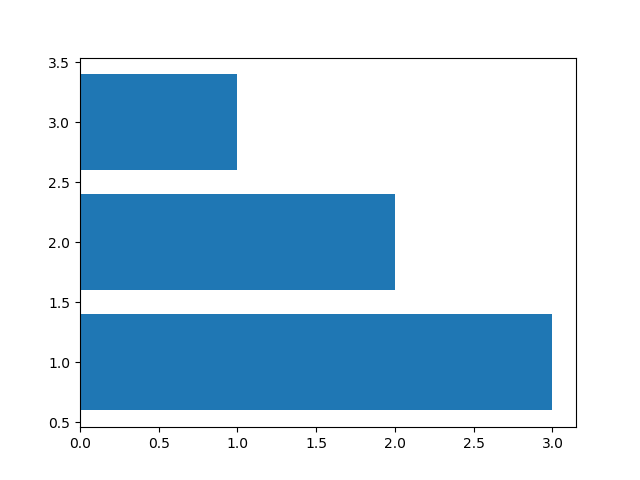
\includegraphics[keepaspectratio]{img/diagrama-barras-horizontales.png}}

}

\caption{Gráfico con matplotlib}

\end{figure}%

\section{Histogramas}\label{histogramas}

\begin{itemize}
\tightlist
\item
  \texttt{hist(x,\ bins)}: Dibuja un histograma con las frecuencias
  resultantes de agrupar los datos de la lista \texttt{x} en las clases
  definidas por la lista \texttt{bins}.
  \href{https://matplotlib.org/api/_as_gen/matplotlib.pyplot.hist.html\#matplotlib.pyplot.hist}{}
\end{itemize}

\begin{Shaded}
\begin{Highlighting}[]
\ImportTok{import}\NormalTok{ numpy }\ImportTok{as}\NormalTok{ np}
\ImportTok{import}\NormalTok{ matplotlib.pyplot }\ImportTok{as}\NormalTok{ plt}
\NormalTok{fig, ax }\OperatorTok{=}\NormalTok{ plt.subplots()}
\NormalTok{x }\OperatorTok{=}\NormalTok{ np.random.normal(}\DecValTok{5}\NormalTok{, }\FloatTok{1.5}\NormalTok{, size}\OperatorTok{=}\DecValTok{1000}\NormalTok{)}
\NormalTok{ax.hist(x, np.arange(}\DecValTok{0}\NormalTok{, }\DecValTok{11}\NormalTok{))}
\NormalTok{plt.show()}
\end{Highlighting}
\end{Shaded}

\begin{figure}[H]

{\centering \pandocbounded{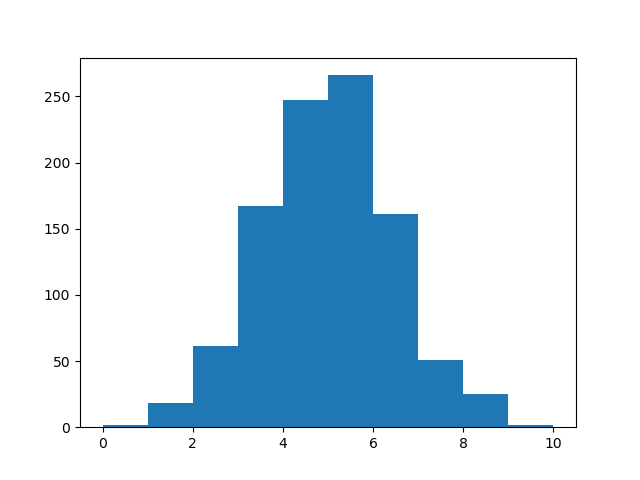
\includegraphics[keepaspectratio]{img/histograma.png}}

}

\caption{Gráfico con matplotlib}

\end{figure}%

\section{Diagramas de sectores}\label{diagramas-de-sectores}

\begin{itemize}
\tightlist
\item
  \texttt{pie(x)}: Dibuja un diagrama de sectores con las frecuencias de
  la lista \texttt{x}.
  \href{https://matplotlib.org/api/_as_gen/matplotlib.pyplot.pie.html\#matplotlib.pyplot.pie}{}
\end{itemize}

\begin{Shaded}
\begin{Highlighting}[]
\ImportTok{import}\NormalTok{ matplotlib.pyplot }\ImportTok{as}\NormalTok{ plt}
\NormalTok{fig, ax }\OperatorTok{=}\NormalTok{ plt.subplots()}
\NormalTok{ax.pie([}\DecValTok{5}\NormalTok{, }\DecValTok{4}\NormalTok{, }\DecValTok{3}\NormalTok{, }\DecValTok{2}\NormalTok{, }\DecValTok{1}\NormalTok{])}
\NormalTok{plt.show()}
\end{Highlighting}
\end{Shaded}

\begin{figure}[H]

{\centering \pandocbounded{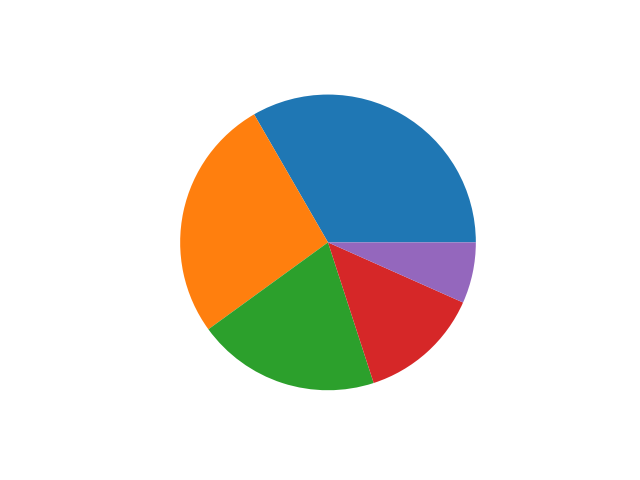
\includegraphics[keepaspectratio]{img/diagrama-sectores.png}}

}

\caption{Gráfico con matplotlib}

\end{figure}%

\section{Diagramas de caja y bigotes}\label{diagramas-de-caja-y-bigotes}

\begin{itemize}
\tightlist
\item
  \texttt{boxplot(x)}: Dibuja un diagrama de caja y bigotes con los
  datos de la lista \texttt{x}.
  \href{https://matplotlib.org/api/_as_gen/matplotlib.pyplot.boxplot.html\#matplotlib.pyplot.boxplot}{}
\end{itemize}

\begin{Shaded}
\begin{Highlighting}[]
\ImportTok{import}\NormalTok{ matplotlib.pyplot }\ImportTok{as}\NormalTok{ plt}
\NormalTok{fig, ax }\OperatorTok{=}\NormalTok{ plt.subplots()}
\NormalTok{ax.boxplot([}\DecValTok{1}\NormalTok{, }\DecValTok{2}\NormalTok{, }\DecValTok{1}\NormalTok{, }\DecValTok{2}\NormalTok{, }\DecValTok{3}\NormalTok{, }\DecValTok{4}\NormalTok{, }\DecValTok{3}\NormalTok{, }\DecValTok{3}\NormalTok{, }\DecValTok{5}\NormalTok{, }\DecValTok{7}\NormalTok{])}
\NormalTok{plt.show()}
\end{Highlighting}
\end{Shaded}

\begin{figure}[H]

{\centering \pandocbounded{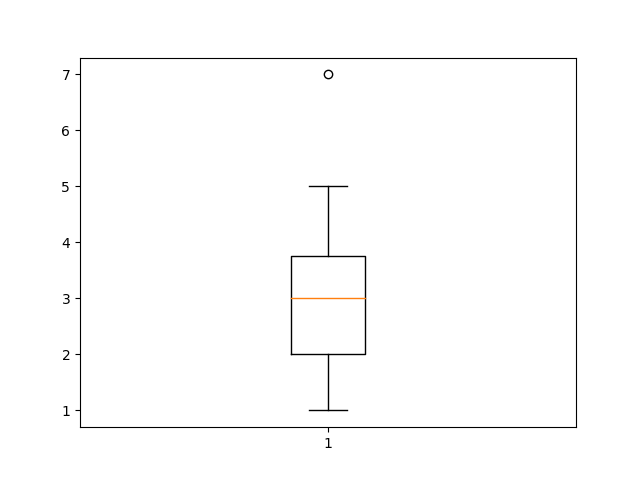
\includegraphics[keepaspectratio]{img/diagrama-caja.png}}

}

\caption{Gráfico con matplotlib}

\end{figure}%

\section{Diagramas de violín}\label{diagramas-de-violuxedn}

\begin{itemize}
\tightlist
\item
  \texttt{violinplot(x)}: Dibuja un diagrama de violín con los datos de
  la lista \texttt{x}.
  \href{https://matplotlib.org/api/_as_gen/matplotlib.pyplot.violinplot.html\#matplotlib.pyplot.violinplot}{}
\end{itemize}

\begin{Shaded}
\begin{Highlighting}[]
\ImportTok{import}\NormalTok{ matplotlib.pyplot }\ImportTok{as}\NormalTok{ plt}
\NormalTok{fig, ax }\OperatorTok{=}\NormalTok{ plt.subplots()}
\NormalTok{ax.violinplot([}\DecValTok{1}\NormalTok{, }\DecValTok{2}\NormalTok{, }\DecValTok{1}\NormalTok{, }\DecValTok{2}\NormalTok{, }\DecValTok{3}\NormalTok{, }\DecValTok{4}\NormalTok{, }\DecValTok{3}\NormalTok{, }\DecValTok{3}\NormalTok{, }\DecValTok{5}\NormalTok{, }\DecValTok{7}\NormalTok{])}
\NormalTok{plt.show()}
\end{Highlighting}
\end{Shaded}

\begin{figure}[H]

{\centering \pandocbounded{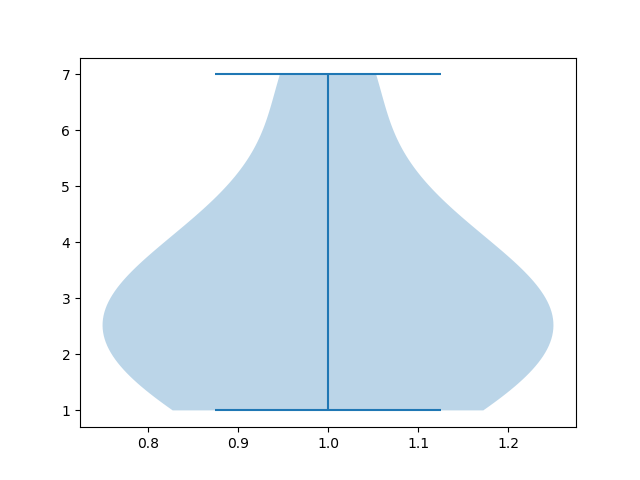
\includegraphics[keepaspectratio]{img/diagrama-violin.png}}

}

\caption{Gráfico con matplotlib}

\end{figure}%

\section{Diagramas de contorno}\label{diagramas-de-contorno}

\begin{itemize}
\tightlist
\item
  \texttt{contourf(x,\ y,\ z)}: Dibuja un diagrama de contorno con las
  curvas de nivel de la superficie dada por los puntos con las
  coordenadas de las listas \texttt{x}, \texttt{y} y \texttt{z} en los
  ejes X, Y y Z respectivamente.
  \href{https://matplotlib.org/api/_as_gen/matplotlib.pyplot.contourf.html\#matplotlib.pyplot.contourf}{}
\end{itemize}

\begin{Shaded}
\begin{Highlighting}[]
\ImportTok{import}\NormalTok{ matplotlib.pyplot }\ImportTok{as}\NormalTok{ plt}
\NormalTok{fig, ax }\OperatorTok{=}\NormalTok{ plt.subplots()}
\NormalTok{x }\OperatorTok{=}\NormalTok{ np.linspace(}\OperatorTok{{-}}\FloatTok{3.0}\NormalTok{, }\FloatTok{3.0}\NormalTok{, }\DecValTok{100}\NormalTok{)}
\NormalTok{y }\OperatorTok{=}\NormalTok{ np.linspace(}\OperatorTok{{-}}\FloatTok{3.0}\NormalTok{, }\FloatTok{3.0}\NormalTok{, }\DecValTok{100}\NormalTok{)}
\NormalTok{x, y }\OperatorTok{=}\NormalTok{ np.meshgrid(x, y)}
\NormalTok{z }\OperatorTok{=}\NormalTok{ np.sqrt(x}\OperatorTok{**}\DecValTok{2} \OperatorTok{+} \DecValTok{2}\OperatorTok{*}\NormalTok{y}\OperatorTok{**}\DecValTok{2}\NormalTok{)}
\NormalTok{ax.contourf(x, y, z)}
\NormalTok{plt.show()}
\end{Highlighting}
\end{Shaded}

\begin{figure}[H]

{\centering \pandocbounded{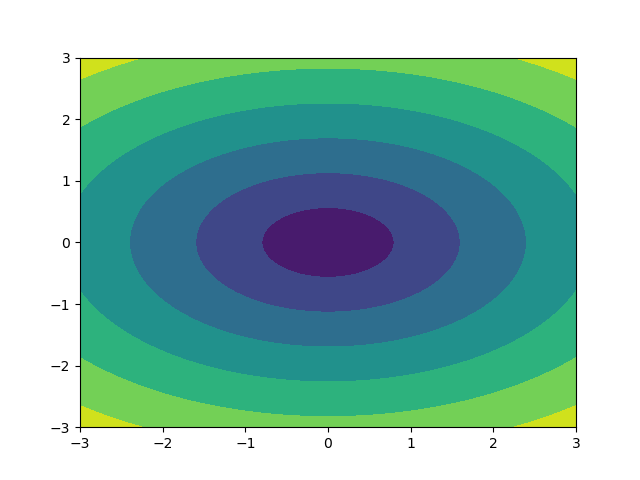
\includegraphics[keepaspectratio]{img/diagrama-contorno.png}}

}

\caption{Gráfico con matplotlib}

\end{figure}%

\section{Mapas de color}\label{mapas-de-color}

\begin{itemize}
\tightlist
\item
  \texttt{imshow(x)}: Dibuja un mapa de color a partir de una matriz
  (array bidimensiona) \texttt{x}.
  \href{https://matplotlib.org/api/_as_gen/matplotlib.pyplot.imshow.html\#matplotlib.pyplot.imshow}{}
\end{itemize}

\begin{Shaded}
\begin{Highlighting}[]
\ImportTok{import}\NormalTok{ matplotlib.pyplot }\ImportTok{as}\NormalTok{ plt}
\NormalTok{fig, ax }\OperatorTok{=}\NormalTok{ plt.subplots()}
\NormalTok{x }\OperatorTok{=}\NormalTok{ np.random.random((}\DecValTok{16}\NormalTok{, }\DecValTok{16}\NormalTok{))}
\NormalTok{ax.imshow(x)}
\NormalTok{plt.show()}
\end{Highlighting}
\end{Shaded}

\begin{figure}[H]

{\centering \pandocbounded{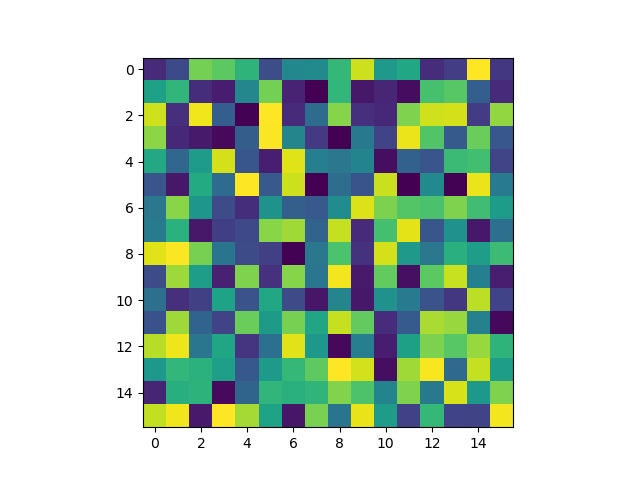
\includegraphics[keepaspectratio]{img/mapa-calor.png}}

}

\caption{Gráfico con matplotlib}

\end{figure}%

\begin{itemize}
\tightlist
\item
  \texttt{hist2d(x,\ y)}: Dibuja un mapa de color que simula un
  histograma bidimensional, donde los colores de los cuadrados dependen
  de las frecuencias de las clases de la muestra dada por las listas
  \texttt{x} e \texttt{y}.
  \href{https://matplotlib.org/api/_as_gen/matplotlib.pyplot.hist2d.html\#matplotlib.pyplot.hist2d}{}
\end{itemize}

\begin{Shaded}
\begin{Highlighting}[]
\ImportTok{import}\NormalTok{ matplotlib.pyplot }\ImportTok{as}\NormalTok{ plt}
\NormalTok{fig, ax }\OperatorTok{=}\NormalTok{ plt.subplots()}
\NormalTok{x, y }\OperatorTok{=}\NormalTok{ np.random.multivariate\_normal(mean}\OperatorTok{=}\NormalTok{[}\FloatTok{0.0}\NormalTok{, }\FloatTok{0.0}\NormalTok{], cov}\OperatorTok{=}\NormalTok{[[}\FloatTok{1.0}\NormalTok{, }\FloatTok{0.4}\NormalTok{], [}\FloatTok{0.4}\NormalTok{, }\FloatTok{0.5}\NormalTok{]], size}\OperatorTok{=}\DecValTok{1000}\NormalTok{).T}
\NormalTok{ax.hist2d(x, y)}
\NormalTok{plt.show()}
\end{Highlighting}
\end{Shaded}

\begin{figure}[H]

{\centering \pandocbounded{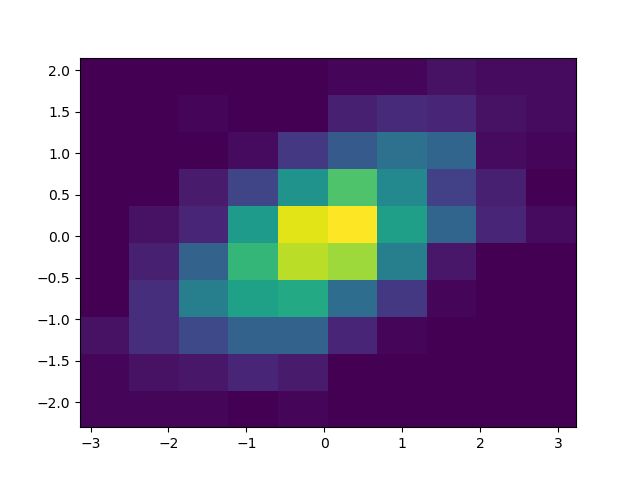
\includegraphics[keepaspectratio]{img/histograma2D.png}}

}

\caption{Gráfico con matplotlib}

\end{figure}%

\section{Cambiar el aspecto de los
gráficos}\label{cambiar-el-aspecto-de-los-gruxe1ficos}

Los gráficos creados con Matplotlib son personalizables y puede
cambiarse el aspecto de casi todos sus elementos. Los elementos que
suelen modificarse más a menudo son:

\begin{itemize}
\tightlist
\item
  Colores
\item
  Marcadores de puntos
\item
  Estilo de líneas
\item
  Títulos
\item
  Ejes
\item
  Leyenda
\item
  Rejilla
\end{itemize}

\section{Colores}\label{colores}

Para cambiar el color de los objetos se utiliza el parámetro
\texttt{color\ =\ nombre-color}, donde \texttt{nombre-color} es una
cadena con el nombre del color de entre los
\href{https://matplotlib.org/3.2.1/gallery/color/named_colors.html}{colores
disponibles}.

\begin{Shaded}
\begin{Highlighting}[]
\ImportTok{import}\NormalTok{ matplotlib.pyplot }\ImportTok{as}\NormalTok{ plt}
\NormalTok{fig, ax }\OperatorTok{=}\NormalTok{ plt.subplots()}
\NormalTok{dias }\OperatorTok{=}\NormalTok{ [}\StringTok{\textquotesingle{}L\textquotesingle{}}\NormalTok{, }\StringTok{\textquotesingle{}M\textquotesingle{}}\NormalTok{, }\StringTok{\textquotesingle{}X\textquotesingle{}}\NormalTok{, }\StringTok{\textquotesingle{}J\textquotesingle{}}\NormalTok{, }\StringTok{\textquotesingle{}V\textquotesingle{}}\NormalTok{, }\StringTok{\textquotesingle{}S\textquotesingle{}}\NormalTok{, }\StringTok{\textquotesingle{}D\textquotesingle{}}\NormalTok{]}
\NormalTok{temperaturas }\OperatorTok{=}\NormalTok{ \{}\StringTok{\textquotesingle{}Madrid\textquotesingle{}}\NormalTok{:[}\FloatTok{28.5}\NormalTok{, }\FloatTok{30.5}\NormalTok{, }\DecValTok{31}\NormalTok{, }\DecValTok{30}\NormalTok{, }\DecValTok{28}\NormalTok{, }\FloatTok{27.5}\NormalTok{, }\FloatTok{30.5}\NormalTok{], }\StringTok{\textquotesingle{}Barcelona\textquotesingle{}}\NormalTok{:[}\FloatTok{24.5}\NormalTok{, }\FloatTok{25.5}\NormalTok{, }\FloatTok{26.5}\NormalTok{, }\DecValTok{25}\NormalTok{, }\FloatTok{26.5}\NormalTok{, }\FloatTok{24.5}\NormalTok{, }\DecValTok{25}\NormalTok{]\}}
\NormalTok{ax.plot(dias, temperaturas[}\StringTok{\textquotesingle{}Madrid\textquotesingle{}}\NormalTok{], color }\OperatorTok{=} \StringTok{\textquotesingle{}tab:purple\textquotesingle{}}\NormalTok{)}
\NormalTok{ax.plot(dias, temperaturas[}\StringTok{\textquotesingle{}Barcelona\textquotesingle{}}\NormalTok{], color }\OperatorTok{=} \StringTok{\textquotesingle{}tab:green\textquotesingle{}}\NormalTok{)}
\NormalTok{plt.show()}
\end{Highlighting}
\end{Shaded}

\begin{figure}[H]

{\centering \pandocbounded{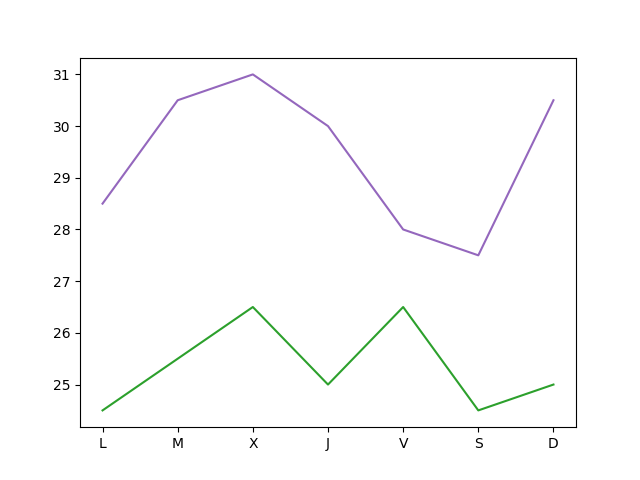
\includegraphics[keepaspectratio]{img/lineas-colores.png}}

}

\caption{Gráfico con matplotlib}

\end{figure}%

\section{Marcadores}\label{marcadores}

Para cambiar la forma de los puntos marcadores se utiliza el parámetro
\texttt{marker\ =\ nombre-marcador} donde \texttt{nombre-marcador} es
una cadena con el nombre del marcador de entre los
\href{https://matplotlib.org/3.2.1/api/markers_api.html}{marcadores
disponibles}

\begin{Shaded}
\begin{Highlighting}[]
\ImportTok{import}\NormalTok{ matplotlib.pyplot }\ImportTok{as}\NormalTok{ plt}
\NormalTok{fig, ax }\OperatorTok{=}\NormalTok{ plt.subplots()}
\NormalTok{dias }\OperatorTok{=}\NormalTok{ [}\StringTok{\textquotesingle{}L\textquotesingle{}}\NormalTok{, }\StringTok{\textquotesingle{}M\textquotesingle{}}\NormalTok{, }\StringTok{\textquotesingle{}X\textquotesingle{}}\NormalTok{, }\StringTok{\textquotesingle{}J\textquotesingle{}}\NormalTok{, }\StringTok{\textquotesingle{}V\textquotesingle{}}\NormalTok{, }\StringTok{\textquotesingle{}S\textquotesingle{}}\NormalTok{, }\StringTok{\textquotesingle{}D\textquotesingle{}}\NormalTok{]}
\NormalTok{temperaturas }\OperatorTok{=}\NormalTok{ \{}\StringTok{\textquotesingle{}Madrid\textquotesingle{}}\NormalTok{:[}\FloatTok{28.5}\NormalTok{, }\FloatTok{30.5}\NormalTok{, }\DecValTok{31}\NormalTok{, }\DecValTok{30}\NormalTok{, }\DecValTok{28}\NormalTok{, }\FloatTok{27.5}\NormalTok{, }\FloatTok{30.5}\NormalTok{], }\StringTok{\textquotesingle{}Barcelona\textquotesingle{}}\NormalTok{:[}\FloatTok{24.5}\NormalTok{, }\FloatTok{25.5}\NormalTok{, }\FloatTok{26.5}\NormalTok{, }\DecValTok{25}\NormalTok{, }\FloatTok{26.5}\NormalTok{, }\FloatTok{24.5}\NormalTok{, }\DecValTok{25}\NormalTok{]\}}
\NormalTok{ax.plot(dias, temperaturas[}\StringTok{\textquotesingle{}Madrid\textquotesingle{}}\NormalTok{], marker }\OperatorTok{=} \StringTok{\textquotesingle{}\^{}\textquotesingle{}}\NormalTok{)}
\NormalTok{ax.plot(dias, temperaturas[}\StringTok{\textquotesingle{}Barcelona\textquotesingle{}}\NormalTok{], marker }\OperatorTok{=} \StringTok{\textquotesingle{}o\textquotesingle{}}\NormalTok{)}
\NormalTok{plt.show()}
\end{Highlighting}
\end{Shaded}

\begin{figure}[H]

{\centering \pandocbounded{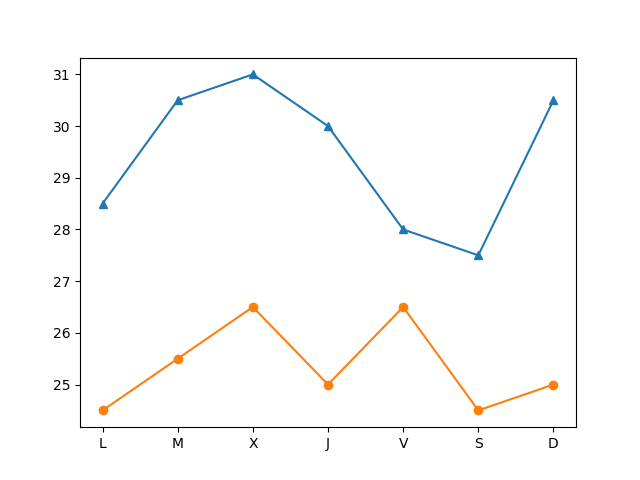
\includegraphics[keepaspectratio]{img/lineas-marcadores.png}}

}

\caption{Gráfico con matplotlib}

\end{figure}%

\section{Líneas}\label{luxedneas}

Para cambiar el estilo de las líneas se utiliza el parámetro
\texttt{linestyle\ =\ nombre-estilo} donde \texttt{nombre-estilo} es una
cadena con el nombre del estilo de entre los
\href{https://matplotlib.org/3.2.1/gallery/lines_bars_and_markers/linestyles.html}{estilos
disponibles}

\begin{Shaded}
\begin{Highlighting}[]
\ImportTok{import}\NormalTok{ matplotlib.pyplot }\ImportTok{as}\NormalTok{ plt}
\NormalTok{fig, ax }\OperatorTok{=}\NormalTok{ plt.subplots()}
\NormalTok{dias }\OperatorTok{=}\NormalTok{ [}\StringTok{\textquotesingle{}L\textquotesingle{}}\NormalTok{, }\StringTok{\textquotesingle{}M\textquotesingle{}}\NormalTok{, }\StringTok{\textquotesingle{}X\textquotesingle{}}\NormalTok{, }\StringTok{\textquotesingle{}J\textquotesingle{}}\NormalTok{, }\StringTok{\textquotesingle{}V\textquotesingle{}}\NormalTok{, }\StringTok{\textquotesingle{}S\textquotesingle{}}\NormalTok{, }\StringTok{\textquotesingle{}D\textquotesingle{}}\NormalTok{]}
\NormalTok{temperaturas }\OperatorTok{=}\NormalTok{ \{}\StringTok{\textquotesingle{}Madrid\textquotesingle{}}\NormalTok{:[}\FloatTok{28.5}\NormalTok{, }\FloatTok{30.5}\NormalTok{, }\DecValTok{31}\NormalTok{, }\DecValTok{30}\NormalTok{, }\DecValTok{28}\NormalTok{, }\FloatTok{27.5}\NormalTok{, }\FloatTok{30.5}\NormalTok{], }\StringTok{\textquotesingle{}Barcelona\textquotesingle{}}\NormalTok{:[}\FloatTok{24.5}\NormalTok{, }\FloatTok{25.5}\NormalTok{, }\FloatTok{26.5}\NormalTok{, }\DecValTok{25}\NormalTok{, }\FloatTok{26.5}\NormalTok{, }\FloatTok{24.5}\NormalTok{, }\DecValTok{25}\NormalTok{]\}}
\NormalTok{ax.plot(dias, temperaturas[}\StringTok{\textquotesingle{}Madrid\textquotesingle{}}\NormalTok{], linestyle }\OperatorTok{=} \StringTok{\textquotesingle{}dashed\textquotesingle{}}\NormalTok{)}
\NormalTok{ax.plot(dias, temperaturas[}\StringTok{\textquotesingle{}Barcelona\textquotesingle{}}\NormalTok{], linestyle }\OperatorTok{=} \StringTok{\textquotesingle{}dotted\textquotesingle{}}\NormalTok{)}
\NormalTok{plt.show()}
\end{Highlighting}
\end{Shaded}

\begin{figure}[H]

{\centering \pandocbounded{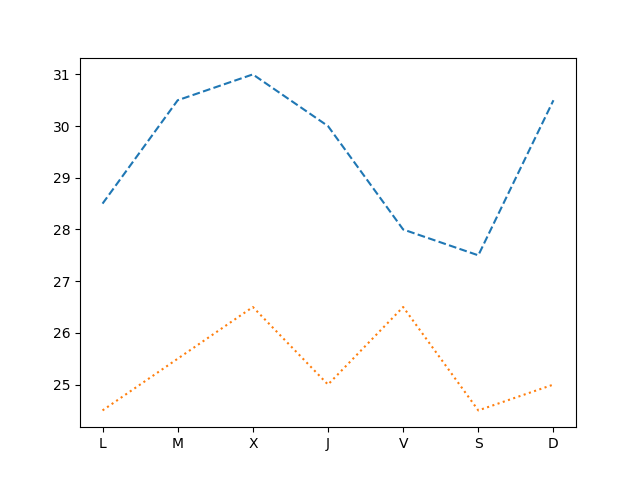
\includegraphics[keepaspectratio]{img/lineas-estilo.png}}

}

\caption{Gráfico con matplotlib}

\end{figure}%

\section{Títulos}\label{tuxedtulos}

Para añadir un título principal al gráfico se utiliza el siguiente
método:

\begin{itemize}
\tightlist
\item
  \texttt{ax.set\_title(titulo,\ loc=alineacion,\ fontdict=fuente)} :
  Añade un título con el contenido de la cadena \texttt{titulo} a los
  ejes \texttt{ax}. El parámetro \texttt{loc} indica la alineación del
  título, que puede ser
  \texttt{\textquotesingle{}left\textquotesingle{}} (izquierda),
  \texttt{\textquotesingle{}center\textquotesingle{}} (centro) o
  \texttt{\textquotesingle{}right\textquotesingle{}} (derecha), y el
  parámetro \texttt{fontdict} indica mediante un diccionario las
  características de la fuente (la el tamaño \texttt{fontisize}, el
  grosor \texttt{fontweight} o el color \texttt{color}).
\end{itemize}

\begin{Shaded}
\begin{Highlighting}[]
\ImportTok{import}\NormalTok{ matplotlib.pyplot }\ImportTok{as}\NormalTok{ plt}
\NormalTok{fig, ax }\OperatorTok{=}\NormalTok{ plt.subplots()}
\NormalTok{dias }\OperatorTok{=}\NormalTok{ [}\StringTok{\textquotesingle{}L\textquotesingle{}}\NormalTok{, }\StringTok{\textquotesingle{}M\textquotesingle{}}\NormalTok{, }\StringTok{\textquotesingle{}X\textquotesingle{}}\NormalTok{, }\StringTok{\textquotesingle{}J\textquotesingle{}}\NormalTok{, }\StringTok{\textquotesingle{}V\textquotesingle{}}\NormalTok{, }\StringTok{\textquotesingle{}S\textquotesingle{}}\NormalTok{, }\StringTok{\textquotesingle{}D\textquotesingle{}}\NormalTok{]}
\NormalTok{temperaturas }\OperatorTok{=}\NormalTok{ \{}\StringTok{\textquotesingle{}Madrid\textquotesingle{}}\NormalTok{:[}\FloatTok{28.5}\NormalTok{, }\FloatTok{30.5}\NormalTok{, }\DecValTok{31}\NormalTok{, }\DecValTok{30}\NormalTok{, }\DecValTok{28}\NormalTok{, }\FloatTok{27.5}\NormalTok{, }\FloatTok{30.5}\NormalTok{], }\StringTok{\textquotesingle{}Barcelona\textquotesingle{}}\NormalTok{:[}\FloatTok{24.5}\NormalTok{, }\FloatTok{25.5}\NormalTok{, }\FloatTok{26.5}\NormalTok{, }\DecValTok{25}\NormalTok{, }\FloatTok{26.5}\NormalTok{, }\FloatTok{24.5}\NormalTok{, }\DecValTok{25}\NormalTok{]\}}
\NormalTok{ax.plot(dias, temperaturas[}\StringTok{\textquotesingle{}Madrid\textquotesingle{}}\NormalTok{])}
\NormalTok{ax.plot(dias, temperaturas[}\StringTok{\textquotesingle{}Barcelona\textquotesingle{}}\NormalTok{])}
\NormalTok{ax.set\_title(}\StringTok{\textquotesingle{}Evolución de la temperatura diaria\textquotesingle{}}\NormalTok{, loc }\OperatorTok{=} \StringTok{"left"}\NormalTok{, fontdict }\OperatorTok{=}\NormalTok{ \{}\StringTok{\textquotesingle{}fontsize\textquotesingle{}}\NormalTok{:}\DecValTok{14}\NormalTok{, }\StringTok{\textquotesingle{}fontweight\textquotesingle{}}\NormalTok{:}\StringTok{\textquotesingle{}bold\textquotesingle{}}\NormalTok{, }\StringTok{\textquotesingle{}color\textquotesingle{}}\NormalTok{:}\StringTok{\textquotesingle{}tab:blue\textquotesingle{}}\NormalTok{\})}
\NormalTok{plt.show()}
\end{Highlighting}
\end{Shaded}

\begin{figure}[H]

{\centering \pandocbounded{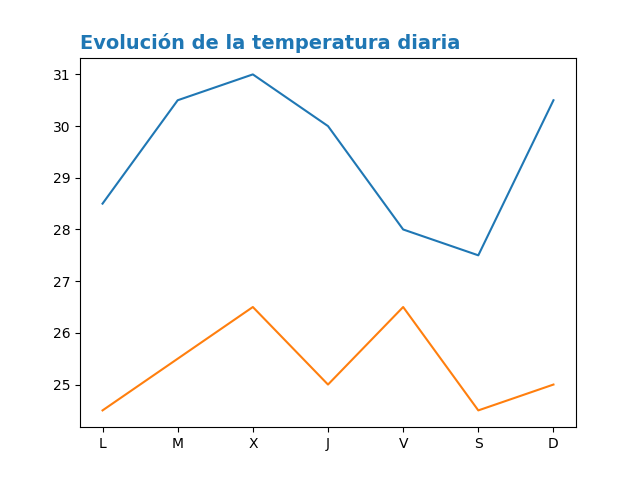
\includegraphics[keepaspectratio]{img/titulo.png}}

}

\caption{Gráfico con matplotlib}

\end{figure}%

\section{Ejes}\label{ejes}

Para cambiar el aspecto de los ejes se suelen utilizar los siguientes
métodos:

\begin{itemize}
\tightlist
\item
  \texttt{ax.set\_xlabel(titulo)} : Añade un título con el contenido de
  la cadena \texttt{titulo} al eje x de \texttt{ax}. Se puede
  personalizar la alineación y la fuente con los mismos parámetros que
  para el título principal.
\item
  \texttt{ax.set\_ylabel(titulo)} : Añade un título con el contenido de
  la cadena \texttt{titulo} al eje y de \texttt{ax}. Se puede
  personalizar la alineación y la fuente con los mismos parámetros que
  para el título principal.
\item
  \texttt{ax.set\_xlim({[}limite-inferior,\ limite-superior{]})} :
  Establece los límites que se muestran en el eje x de \texttt{ax}.
\item
  \texttt{ax.set\_ylim({[}limite-inferior,\ limite-superior{]})} :
  Establece los límites que se muestran en el eje y de \texttt{ax}.
\item
  \texttt{ax.set\_xticks(marcas)} : Dibuja marcas en el eje x de
  \texttt{ax} en las posiciones indicadas en la lista \texttt{marcas}.
\item
  \texttt{ax.set\_yticks(marcas)} : Dibuja marcas en el eje y de
  \texttt{ax} en las posiciones indicadas en la lista \texttt{marcas}.
\item
  \texttt{ax.set\_xscale(escala)} : Establece la escala del eje x de
  \texttt{ax}, donde el parámetro \texttt{escala} puede ser
  \texttt{\textquotesingle{}linear\textquotesingle{}} (lineal) o
  \texttt{\textquotesingle{}log\textquotesingle{}} (logarítmica).\\
\item
  \texttt{ax.set\_yscale(escala)} : Establece la escala del eje y de
  \texttt{ax}, donde el parámetro \texttt{escala} puede ser
  \texttt{\textquotesingle{}linear\textquotesingle{}} (lineal) o
  \texttt{\textquotesingle{}log\textquotesingle{}} (logarítmica).
\end{itemize}

\begin{Shaded}
\begin{Highlighting}[]
\ImportTok{import}\NormalTok{ matplotlib.pyplot }\ImportTok{as}\NormalTok{ plt}
\NormalTok{fig, ax }\OperatorTok{=}\NormalTok{ plt.subplots()}
\NormalTok{dias }\OperatorTok{=}\NormalTok{ [}\StringTok{\textquotesingle{}L\textquotesingle{}}\NormalTok{, }\StringTok{\textquotesingle{}M\textquotesingle{}}\NormalTok{, }\StringTok{\textquotesingle{}X\textquotesingle{}}\NormalTok{, }\StringTok{\textquotesingle{}J\textquotesingle{}}\NormalTok{, }\StringTok{\textquotesingle{}V\textquotesingle{}}\NormalTok{, }\StringTok{\textquotesingle{}S\textquotesingle{}}\NormalTok{, }\StringTok{\textquotesingle{}D\textquotesingle{}}\NormalTok{]}
\NormalTok{temperaturas }\OperatorTok{=}\NormalTok{ \{}\StringTok{\textquotesingle{}Madrid\textquotesingle{}}\NormalTok{:[}\FloatTok{28.5}\NormalTok{, }\FloatTok{30.5}\NormalTok{, }\DecValTok{31}\NormalTok{, }\DecValTok{30}\NormalTok{, }\DecValTok{28}\NormalTok{, }\FloatTok{27.5}\NormalTok{, }\FloatTok{30.5}\NormalTok{], }\StringTok{\textquotesingle{}Barcelona\textquotesingle{}}\NormalTok{:[}\FloatTok{24.5}\NormalTok{, }\FloatTok{25.5}\NormalTok{, }\FloatTok{26.5}\NormalTok{, }\DecValTok{25}\NormalTok{, }\FloatTok{26.5}\NormalTok{, }\FloatTok{24.5}\NormalTok{, }\DecValTok{25}\NormalTok{]\}}
\NormalTok{ax.plot(dias, temperaturas[}\StringTok{\textquotesingle{}Madrid\textquotesingle{}}\NormalTok{])}
\NormalTok{ax.plot(dias, temperaturas[}\StringTok{\textquotesingle{}Barcelona\textquotesingle{}}\NormalTok{])}
\NormalTok{ax.set\_xlabel(}\StringTok{"Días"}\NormalTok{, fontdict }\OperatorTok{=}\NormalTok{ \{}\StringTok{\textquotesingle{}fontsize\textquotesingle{}}\NormalTok{:}\DecValTok{14}\NormalTok{, }\StringTok{\textquotesingle{}fontweight\textquotesingle{}}\NormalTok{:}\StringTok{\textquotesingle{}bold\textquotesingle{}}\NormalTok{, }\StringTok{\textquotesingle{}color\textquotesingle{}}\NormalTok{:}\StringTok{\textquotesingle{}tab:blue\textquotesingle{}}\NormalTok{\})}
\NormalTok{ax.set\_ylabel(}\StringTok{"Temperatura ºC"}\NormalTok{)}
\NormalTok{ax.set\_ylim([}\DecValTok{20}\NormalTok{,}\DecValTok{35}\NormalTok{])}
\NormalTok{ax.set\_yticks(}\BuiltInTok{range}\NormalTok{(}\DecValTok{20}\NormalTok{, }\DecValTok{35}\NormalTok{))}
\NormalTok{plt.show()}
\end{Highlighting}
\end{Shaded}

\begin{figure}[H]

{\centering \pandocbounded{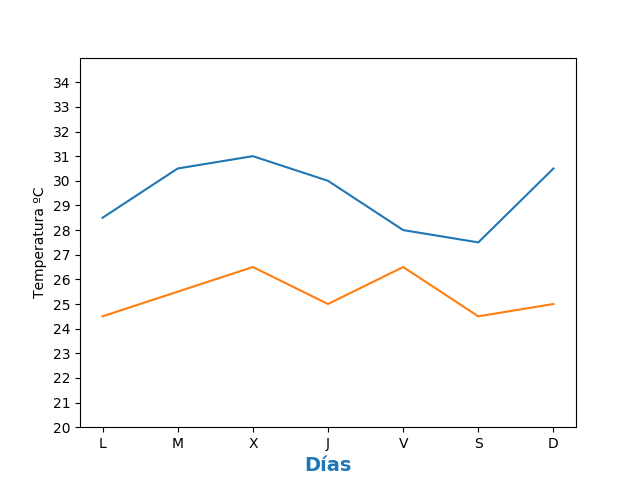
\includegraphics[keepaspectratio]{img/ejes.png}}

}

\caption{Gráfico con matplotlib}

\end{figure}%

\section{Leyenda}\label{leyenda}

Para añadir una leyenda a un gráfico se utiliza el siguiente método:

\begin{itemize}
\tightlist
\item
  \texttt{ax.legend(leyendas,\ loc\ =\ posición)} : Dibuja un leyenda en
  los ejes \texttt{ax} con los nombres indicados en la lista
  \texttt{leyendas}. El parámetro \texttt{loc} indica la posición en la
  que se dibuja la leyenda y puede ser
  \texttt{\textquotesingle{}upper\ left\textquotesingle{}} (arriba
  izquierda), \texttt{\textquotesingle{}upper\ center\textquotesingle{}}
  (arriba centro),
  \texttt{\textquotesingle{}upper\ right\textquotesingle{}} (arriba
  derecha), \texttt{\textquotesingle{}center\ left\textquotesingle{}}
  (centro izquierda),
  \texttt{\textquotesingle{}center\textquotesingle{}} (centro),
  \texttt{\textquotesingle{}center\ right\textquotesingle{}} (centro
  derecha), \texttt{\textquotesingle{}lower\ left\textquotesingle{}}
  (abajo izquierda),
  \texttt{\textquotesingle{}lower\ center\textquotesingle{}} (abajo
  centro), \texttt{\textquotesingle{}lower\ right\textquotesingle{}}
  (abajo derecha). Se puede omitir la lista \texttt{leyendas} si se
  indica la leyenda de cada serie en la función que la dibuja mediante
  el parámetro \texttt{label}.
\end{itemize}

\begin{Shaded}
\begin{Highlighting}[]
\ImportTok{import}\NormalTok{ matplotlib.pyplot }\ImportTok{as}\NormalTok{ plt}
\NormalTok{fig, ax }\OperatorTok{=}\NormalTok{ plt.subplots()}
\NormalTok{dias }\OperatorTok{=}\NormalTok{ [}\StringTok{\textquotesingle{}L\textquotesingle{}}\NormalTok{, }\StringTok{\textquotesingle{}M\textquotesingle{}}\NormalTok{, }\StringTok{\textquotesingle{}X\textquotesingle{}}\NormalTok{, }\StringTok{\textquotesingle{}J\textquotesingle{}}\NormalTok{, }\StringTok{\textquotesingle{}V\textquotesingle{}}\NormalTok{, }\StringTok{\textquotesingle{}S\textquotesingle{}}\NormalTok{, }\StringTok{\textquotesingle{}D\textquotesingle{}}\NormalTok{]}
\NormalTok{temperaturas }\OperatorTok{=}\NormalTok{ \{}\StringTok{\textquotesingle{}Madrid\textquotesingle{}}\NormalTok{:[}\FloatTok{28.5}\NormalTok{, }\FloatTok{30.5}\NormalTok{, }\DecValTok{31}\NormalTok{, }\DecValTok{30}\NormalTok{, }\DecValTok{28}\NormalTok{, }\FloatTok{27.5}\NormalTok{, }\FloatTok{30.5}\NormalTok{], }\StringTok{\textquotesingle{}Barcelona\textquotesingle{}}\NormalTok{:[}\FloatTok{24.5}\NormalTok{, }\FloatTok{25.5}\NormalTok{, }\FloatTok{26.5}\NormalTok{, }\DecValTok{25}\NormalTok{, }\FloatTok{26.5}\NormalTok{, }\FloatTok{24.5}\NormalTok{, }\DecValTok{25}\NormalTok{]\}}
\NormalTok{ax.plot(dias, temperaturas[}\StringTok{\textquotesingle{}Madrid\textquotesingle{}}\NormalTok{], label }\OperatorTok{=} \StringTok{\textquotesingle{}Madrid\textquotesingle{}}\NormalTok{)}
\NormalTok{ax.plot(dias, temperaturas[}\StringTok{\textquotesingle{}Barcelona\textquotesingle{}}\NormalTok{], label }\OperatorTok{=} \StringTok{\textquotesingle{}Barcelona\textquotesingle{}}\NormalTok{)}
\NormalTok{ax.legend(loc }\OperatorTok{=} \StringTok{\textquotesingle{}upper right\textquotesingle{}}\NormalTok{)}
\NormalTok{plt.show()}
\end{Highlighting}
\end{Shaded}

\begin{figure}[H]

{\centering \pandocbounded{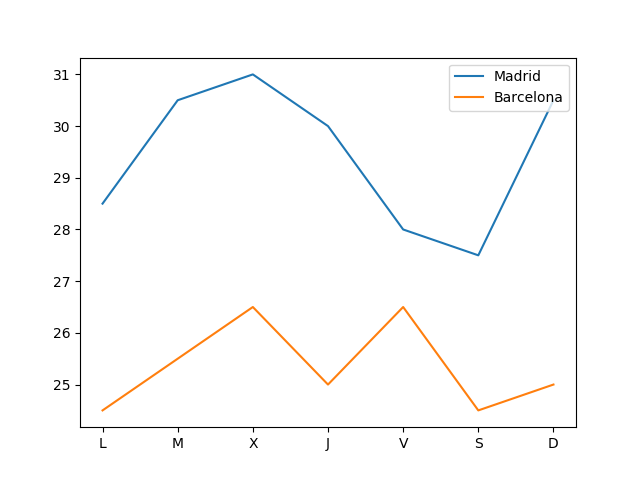
\includegraphics[keepaspectratio]{img/leyenda.png}}

}

\caption{Gráfico con matplotlib}

\end{figure}%

\section{Rejilla}\label{rejilla}

\texttt{ax.grid(axis=ejes,\ color=color,\ linestyle=estilo)} : Dibuja
una rejilla en los ejes de \texttt{ax}. El parámetro \texttt{axis}
indica los ejes sobre los que se dibuja la regilla y puede ser
\texttt{\textquotesingle{}x\textquotesingle{}} (eje x),
\texttt{\textquotesingle{}y\textquotesingle{}} (eje y) o
\texttt{\textquotesingle{}both\textquotesingle{}} (ambos). Los
parámetros \texttt{color} y \texttt{linestyle} establecen el color y el
estilo de las líneas de la rejilla, y pueden tomar los mismos valores
vistos en los apartados de colores y líneas.

\begin{Shaded}
\begin{Highlighting}[]
\ImportTok{import}\NormalTok{ matplotlib.pyplot }\ImportTok{as}\NormalTok{ plt}
\NormalTok{fig, ax }\OperatorTok{=}\NormalTok{ plt.subplots()}
\NormalTok{dias }\OperatorTok{=}\NormalTok{ [}\StringTok{\textquotesingle{}L\textquotesingle{}}\NormalTok{, }\StringTok{\textquotesingle{}M\textquotesingle{}}\NormalTok{, }\StringTok{\textquotesingle{}X\textquotesingle{}}\NormalTok{, }\StringTok{\textquotesingle{}J\textquotesingle{}}\NormalTok{, }\StringTok{\textquotesingle{}V\textquotesingle{}}\NormalTok{, }\StringTok{\textquotesingle{}S\textquotesingle{}}\NormalTok{, }\StringTok{\textquotesingle{}D\textquotesingle{}}\NormalTok{]}
\NormalTok{temperaturas }\OperatorTok{=}\NormalTok{ \{}\StringTok{\textquotesingle{}Madrid\textquotesingle{}}\NormalTok{:[}\FloatTok{28.5}\NormalTok{, }\FloatTok{30.5}\NormalTok{, }\DecValTok{31}\NormalTok{, }\DecValTok{30}\NormalTok{, }\DecValTok{28}\NormalTok{, }\FloatTok{27.5}\NormalTok{, }\FloatTok{30.5}\NormalTok{], }\StringTok{\textquotesingle{}Barcelona\textquotesingle{}}\NormalTok{:[}\FloatTok{24.5}\NormalTok{, }\FloatTok{25.5}\NormalTok{, }\FloatTok{26.5}\NormalTok{, }\DecValTok{25}\NormalTok{, }\FloatTok{26.5}\NormalTok{, }\FloatTok{24.5}\NormalTok{, }\DecValTok{25}\NormalTok{]\}}
\NormalTok{ax.plot(dias, temperaturas[}\StringTok{\textquotesingle{}Madrid\textquotesingle{}}\NormalTok{])}
\NormalTok{ax.plot(dias, temperaturas[}\StringTok{\textquotesingle{}Barcelona\textquotesingle{}}\NormalTok{])}
\NormalTok{ax.grid(axis }\OperatorTok{=} \StringTok{\textquotesingle{}y\textquotesingle{}}\NormalTok{, color }\OperatorTok{=} \StringTok{\textquotesingle{}gray\textquotesingle{}}\NormalTok{, linestyle }\OperatorTok{=} \StringTok{\textquotesingle{}dashed\textquotesingle{}}\NormalTok{)}
\NormalTok{plt.show()}
\end{Highlighting}
\end{Shaded}

\begin{figure}[H]

{\centering \pandocbounded{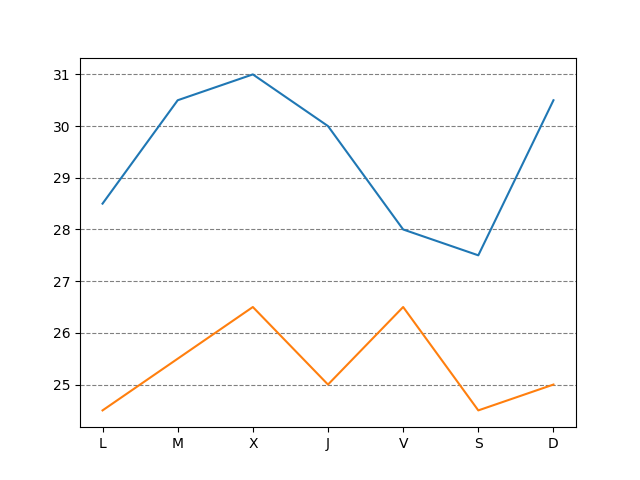
\includegraphics[keepaspectratio]{img/rejilla.png}}

}

\caption{Gráfico con matplotlib}

\end{figure}%

\section{Múltiples gráficos}\label{muxfaltiples-gruxe1ficos}

Es posible dibujar varios gráficos en distintos ejes en una misma figura
organizados en forma de tabla. Para ello, cuando se inicializa la figura
y los ejes, hay que pasarle a la función \texttt{subplots} el número de
filas y columnas de la tabla que contendrá los gráficos. Con esto los
distintos ejes se organizan en un array y se puede acceder a cada uno de
ellos a través de sus índices. Si se quiere que los distintos ejes
compartan los mismos límites para los ejes se pueden pasar los
parámetros \texttt{sharex\ =\ True} para el eje x o
\texttt{sharey\ =\ True} para el eje y.

\begin{Shaded}
\begin{Highlighting}[]
\ImportTok{import}\NormalTok{ matplotlib.pyplot }\ImportTok{as}\NormalTok{ plt}
\NormalTok{fig, ax }\OperatorTok{=}\NormalTok{ plt.subplots(}\DecValTok{2}\NormalTok{, }\DecValTok{2}\NormalTok{, sharey }\OperatorTok{=} \VariableTok{True}\NormalTok{)}
\NormalTok{dias }\OperatorTok{=}\NormalTok{ [}\StringTok{\textquotesingle{}L\textquotesingle{}}\NormalTok{, }\StringTok{\textquotesingle{}M\textquotesingle{}}\NormalTok{, }\StringTok{\textquotesingle{}X\textquotesingle{}}\NormalTok{, }\StringTok{\textquotesingle{}J\textquotesingle{}}\NormalTok{, }\StringTok{\textquotesingle{}V\textquotesingle{}}\NormalTok{, }\StringTok{\textquotesingle{}S\textquotesingle{}}\NormalTok{, }\StringTok{\textquotesingle{}D\textquotesingle{}}\NormalTok{]}
\NormalTok{temperaturas }\OperatorTok{=}\NormalTok{ \{}\StringTok{\textquotesingle{}Madrid\textquotesingle{}}\NormalTok{:[}\FloatTok{28.5}\NormalTok{, }\FloatTok{30.5}\NormalTok{, }\DecValTok{31}\NormalTok{, }\DecValTok{30}\NormalTok{, }\DecValTok{28}\NormalTok{, }\FloatTok{27.5}\NormalTok{, }\FloatTok{30.5}\NormalTok{], }\StringTok{\textquotesingle{}Barcelona\textquotesingle{}}\NormalTok{:[}\FloatTok{24.5}\NormalTok{, }\FloatTok{25.5}\NormalTok{, }\FloatTok{26.5}\NormalTok{, }\DecValTok{25}\NormalTok{, }\FloatTok{26.5}\NormalTok{, }\FloatTok{24.5}\NormalTok{, }\DecValTok{25}\NormalTok{]\}}
\NormalTok{ax[}\DecValTok{0}\NormalTok{, }\DecValTok{0}\NormalTok{].plot(dias, temperaturas[}\StringTok{\textquotesingle{}Madrid\textquotesingle{}}\NormalTok{])}
\NormalTok{ax[}\DecValTok{0}\NormalTok{, }\DecValTok{1}\NormalTok{].plot(dias, temperaturas[}\StringTok{\textquotesingle{}Barcelona\textquotesingle{}}\NormalTok{], color }\OperatorTok{=} \StringTok{\textquotesingle{}tab:orange\textquotesingle{}}\NormalTok{)}
\NormalTok{ax[}\DecValTok{1}\NormalTok{, }\DecValTok{0}\NormalTok{].bar(dias, temperaturas[}\StringTok{\textquotesingle{}Madrid\textquotesingle{}}\NormalTok{])}
\NormalTok{ax[}\DecValTok{1}\NormalTok{, }\DecValTok{1}\NormalTok{].bar(dias, temperaturas[}\StringTok{\textquotesingle{}Barcelona\textquotesingle{}}\NormalTok{], color }\OperatorTok{=} \StringTok{\textquotesingle{}tab:orange\textquotesingle{}}\NormalTok{)}
\NormalTok{plt.show()}
\end{Highlighting}
\end{Shaded}

\begin{figure}[H]

{\centering \pandocbounded{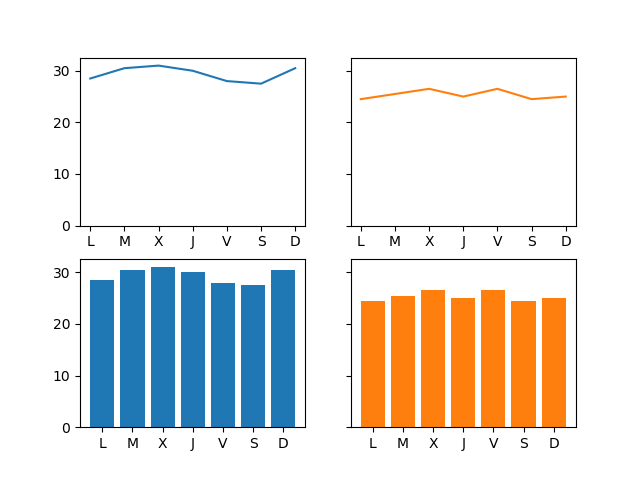
\includegraphics[keepaspectratio]{img/multiples-graficos.png}}

}

\caption{Gráfico con matplotlib}

\end{figure}%

\section{Integración con Pandas}\label{integraciuxf3n-con-pandas}

Matplotlib se integra a la perfección con la librería Pandas,
permitiendo dibujar gráficos a partir de los datos de las series y
DataFrames de Pandas.

\begin{itemize}
\tightlist
\item
  \texttt{df.plot(kind=tipo,\ x=columnax,\ y=columnay,\ ax=ejes)} :
  Dibuja un diagrama del tipo indicado por el parámetro \texttt{kind} en
  los ejes indicados en el parámetro \texttt{ax}, representando en el
  eje x la columna del parámetro \texttt{x} y en el eje y la columna del
  parámetro \texttt{y}. El parámetro \texttt{kind} puede tomar como
  argumentos \texttt{\textquotesingle{}line\textquotesingle{}} (lineas),
  \texttt{\textquotesingle{}scatter\textquotesingle{}} (puntos),
  \texttt{\textquotesingle{}bar\textquotesingle{}} (barras verticales),
  \texttt{\textquotesingle{}barh\textquotesingle{}} (barras
  horizontales), \texttt{\textquotesingle{}hist\textquotesingle{}}
  (histograma), \texttt{\textquotesingle{}box\textquotesingle{}}
  (cajas), \texttt{\textquotesingle{}density\textquotesingle{}}
  (densidad), \texttt{\textquotesingle{}area\textquotesingle{}} (area) o
  \texttt{\textquotesingle{}pie\textquotesingle{}} (sectores). Es
  posible pasar otros parámetros para indicar el color, el marcador o el
  estilo de línea como se vió en los apartados anteriores.
\end{itemize}

\begin{Shaded}
\begin{Highlighting}[]
\ImportTok{import}\NormalTok{ pandas }\ImportTok{as}\NormalTok{ pd }
\ImportTok{import}\NormalTok{ matplotlib.pyplot }\ImportTok{as}\NormalTok{ plt}
\NormalTok{df }\OperatorTok{=}\NormalTok{ pd.DataFrame(\{}\StringTok{\textquotesingle{}Días\textquotesingle{}}\NormalTok{:[}\StringTok{\textquotesingle{}L\textquotesingle{}}\NormalTok{, }\StringTok{\textquotesingle{}M\textquotesingle{}}\NormalTok{, }\StringTok{\textquotesingle{}X\textquotesingle{}}\NormalTok{, }\StringTok{\textquotesingle{}J\textquotesingle{}}\NormalTok{, }\StringTok{\textquotesingle{}V\textquotesingle{}}\NormalTok{, }\StringTok{\textquotesingle{}S\textquotesingle{}}\NormalTok{, }\StringTok{\textquotesingle{}D\textquotesingle{}}\NormalTok{], }
                   \StringTok{\textquotesingle{}Madrid\textquotesingle{}}\NormalTok{:[}\FloatTok{28.5}\NormalTok{, }\FloatTok{30.5}\NormalTok{, }\DecValTok{31}\NormalTok{, }\DecValTok{30}\NormalTok{, }\DecValTok{28}\NormalTok{, }\FloatTok{27.5}\NormalTok{, }\FloatTok{30.5}\NormalTok{], }
                   \StringTok{\textquotesingle{}Barcelona\textquotesingle{}}\NormalTok{:[}\FloatTok{24.5}\NormalTok{, }\FloatTok{25.5}\NormalTok{, }\FloatTok{26.5}\NormalTok{, }\DecValTok{25}\NormalTok{, }\FloatTok{26.5}\NormalTok{, }\FloatTok{24.5}\NormalTok{, }\DecValTok{25}\NormalTok{]\})}
\NormalTok{fig, ax }\OperatorTok{=}\NormalTok{ plt.subplots()}
\NormalTok{df.plot(x }\OperatorTok{=} \StringTok{\textquotesingle{}Días\textquotesingle{}}\NormalTok{, y }\OperatorTok{=} \StringTok{\textquotesingle{}Madrid\textquotesingle{}}\NormalTok{, ax }\OperatorTok{=}\NormalTok{ ax)}
\NormalTok{df.plot(x }\OperatorTok{=} \StringTok{\textquotesingle{}Días\textquotesingle{}}\NormalTok{, y }\OperatorTok{=} \StringTok{\textquotesingle{}Barcelona\textquotesingle{}}\NormalTok{, ax }\OperatorTok{=}\NormalTok{ ax)}
\NormalTok{plt.show()}
\end{Highlighting}
\end{Shaded}

\begin{figure}[H]

{\centering \pandocbounded{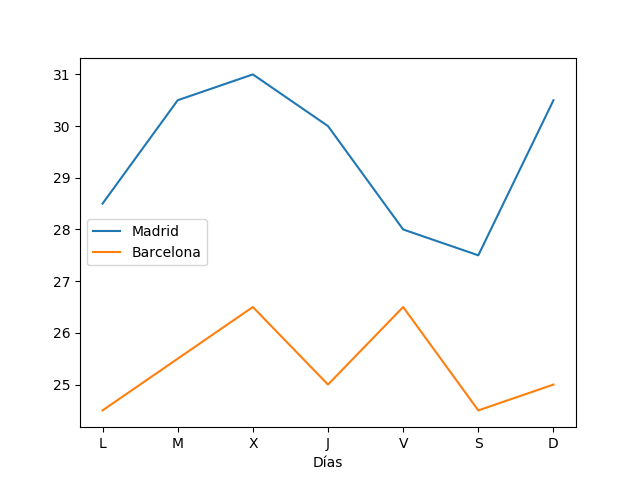
\includegraphics[keepaspectratio]{img/matplotlib-pandas.png}}

}

\caption{Gráfico con matplotlib}

\end{figure}%

Si no se indican los parámetros \texttt{x} e \texttt{y} se representa el
índice de las filas en el eje x y una serie por cada columna del
Dataframe. Las columnas no numéricas se ignoran.

\begin{Shaded}
\begin{Highlighting}[]
\ImportTok{import}\NormalTok{ pandas }\ImportTok{as}\NormalTok{ pd }
\ImportTok{import}\NormalTok{ matplotlib.pyplot }\ImportTok{as}\NormalTok{ plt}
\NormalTok{df }\OperatorTok{=}\NormalTok{ pd.DataFrame(\{}\StringTok{\textquotesingle{}Días\textquotesingle{}}\NormalTok{:[}\StringTok{\textquotesingle{}L\textquotesingle{}}\NormalTok{, }\StringTok{\textquotesingle{}M\textquotesingle{}}\NormalTok{, }\StringTok{\textquotesingle{}X\textquotesingle{}}\NormalTok{, }\StringTok{\textquotesingle{}J\textquotesingle{}}\NormalTok{, }\StringTok{\textquotesingle{}V\textquotesingle{}}\NormalTok{, }\StringTok{\textquotesingle{}S\textquotesingle{}}\NormalTok{, }\StringTok{\textquotesingle{}D\textquotesingle{}}\NormalTok{], }
                   \StringTok{\textquotesingle{}Madrid\textquotesingle{}}\NormalTok{:[}\FloatTok{28.5}\NormalTok{, }\FloatTok{30.5}\NormalTok{, }\DecValTok{31}\NormalTok{, }\DecValTok{30}\NormalTok{, }\DecValTok{28}\NormalTok{, }\FloatTok{27.5}\NormalTok{, }\FloatTok{30.5}\NormalTok{], }
                   \StringTok{\textquotesingle{}Barcelona\textquotesingle{}}\NormalTok{:[}\FloatTok{24.5}\NormalTok{, }\FloatTok{25.5}\NormalTok{, }\FloatTok{26.5}\NormalTok{, }\DecValTok{25}\NormalTok{, }\FloatTok{26.5}\NormalTok{, }\FloatTok{24.5}\NormalTok{, }\DecValTok{25}\NormalTok{]\})}
\NormalTok{df }\OperatorTok{=}\NormalTok{ df.set\_index(}\StringTok{\textquotesingle{}Días\textquotesingle{}}\NormalTok{)}
\NormalTok{fig, ax }\OperatorTok{=}\NormalTok{ plt.subplots()}
\NormalTok{df.plot(ax }\OperatorTok{=}\NormalTok{ ax)}
\NormalTok{plt.show()}
\end{Highlighting}
\end{Shaded}

\begin{figure}[H]

{\centering \pandocbounded{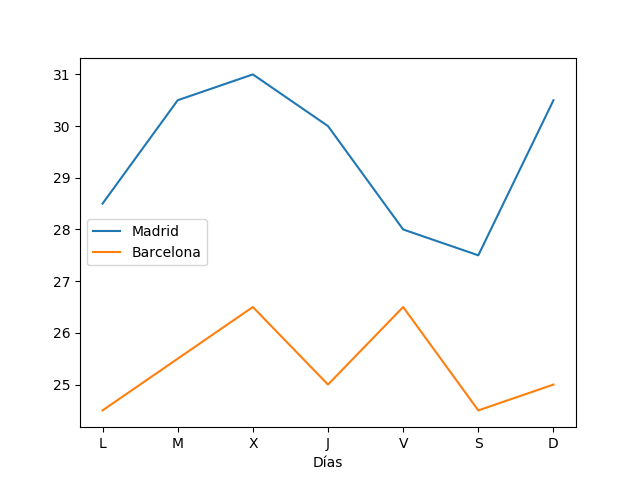
\includegraphics[keepaspectratio]{img/matplotlib-pandas2.png}}

}

\caption{Gráfico con matplotlib}

\end{figure}%

\cleardoublepage
\phantomsection
\addcontentsline{toc}{part}{Apéndices}
\appendix

\chapter{Depuración de código}\label{depuraciuxf3n-de-cuxf3digo}

\section{Depuración de programas}\label{depuraciuxf3n-de-programas}

La depuración es una técnica que permite \emph{trazar} un programa, es
decir, seguir el flujo de ejecución de un programa paso a paso,
ejecutando una instrucción en cada paso, y observar el estado de sus
variables.

Cuando un programa tiene cierta complejidad, la depuración es
imprescindible pare detectar posibles errores.

Python dispone del módulo \texttt{pyd} para depurar programas, pero es
mucho más cómodo utilizar algún entorno de desarrollo que incorpore la
depuración, como por ejemplo Visual Studio Code.

\subsection{Comandos de depuración}\label{comandos-de-depuraciuxf3n}

\begin{itemize}
\tightlist
\item
  \textbf{Establecer punto de parada}: Detiene la ejecución del programa
  en una línea concreta de código.
\item
  \textbf{Continuar la ejecución}: Continúa la ejecución del programa
  hasta el siguiente punto de parada o hasta que finalice.
\item
  \textbf{Próximo paso}: Ejecuta la siguiente línea de código y para la
  ejecución.
\item
  \textbf{Próximo paso con entrada en función}: Ejecuta la siguiente
  línea de código. Si se trata de una llamada a una función entonces
  ejecuta la primera instrucción de la función y para la ejecución.
\item
  \textbf{Próximo paso con salida de función}: Ejecuta lo que queda de
  la función actual y para la ejecución.
\item
  \textbf{Terminar la depuración}: Termina la depuración.
\end{itemize}

\subsection{Depuración en Visual Studio
Code}\label{depuraciuxf3n-en-visual-studio-code}

Antes de iniciar la depuración de un programa en VSCode hay que
establecer algún punto de parada. Para ello basta con hacer click en le
margen izquierdo de la ventana con del código a la altura de la línea
donde se quiere parar la ejecución del programa.

\begin{figure}[H]

{\centering \pandocbounded{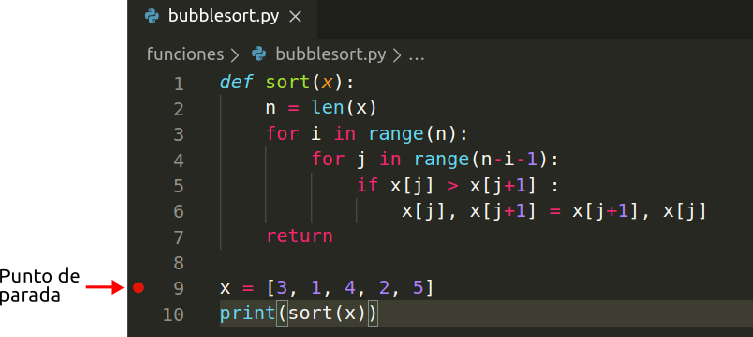
\includegraphics[keepaspectratio]{img/break-point.png}}

}

\caption{Punto de parada en Visual Studio Code}

\end{figure}%

Para iniciar la depuración de un programa en VSCode hay que hacer clic
sobre el botón
\pandocbounded{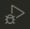
\includegraphics[keepaspectratio,alt={Visual Studio Code debbuger}]{img/debug-button.png}}
o pulsar la combinación de teclas (Ctr+Shift+D).

La primera vez que depuremos un programa tendremos que crear un fichero
de configuración del depurador (\texttt{launch.json}). Para ello hay que
hacer clic en el botón \texttt{Run\ and\ Debug}. VSCode mostrará los
distintos ficheros de configuración disponibles y debe seleccionarse el
más adecuado para el tipo de programa a depurar. Para programas simples
se debe seleccionar \texttt{Python\ file}.

La depuración comenzará iniciando la ejecución del programa desde el
inicio hasta el primer punto de parada que encuentre.

Una vez iniciado el proceso de depuración, se puede avanzar en la
ejecución del programa haciendo uso de la barra de depuración que
contiene botones con los principales comandos de depuración.

\begin{figure}[H]

{\centering \pandocbounded{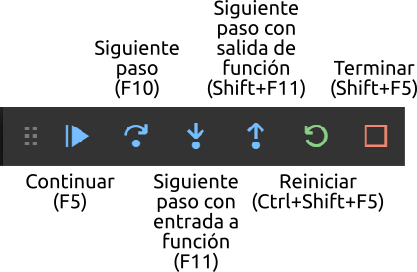
\includegraphics[keepaspectratio]{img/debbuger-bar.png}}

}

\caption{Barra de depuración de Visual Studio Code}

\end{figure}%

Durante la ejecución del programa, se puede ver el contenido de las
variables del programa en la ventana del estado de las variables.

El usuario también puede introducir expresiones y ver cómo se evalúan
durante la ejecución del programa en la ventana de vista de expresiones.

\begin{figure}[H]

{\centering \pandocbounded{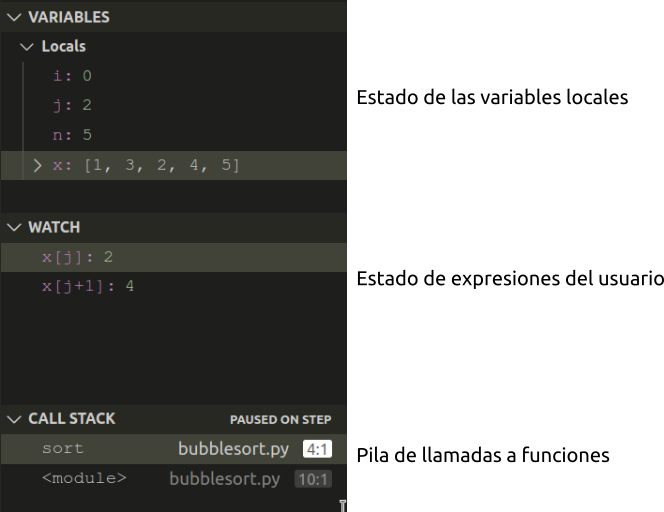
\includegraphics[keepaspectratio]{img/debbuger-estado-variables.png}}

}

\caption{Ventana de estado de variables de Visual Studio Code}

\end{figure}%

\chapter{Bibliografía}\label{bibliografuxeda}

\section{Referencias}\label{referencias}

\subsection{Webs}\label{webs}

\begin{itemize}
\tightlist
\item
  \href{https://www.python.org/}{Python} Sitio web de Python.
\item
  \href{https://repl.it/}{Repl.it} Entorno de desarrollo web para varios
  lenguajes, incluido Python.
\item
  \href{http://pythontutor.com/}{Python tutor} Sitio web que permite
  visualizar la ejecución el código Python.
\end{itemize}

\subsection{Libros y manuales}\label{libros-y-manuales}

\begin{itemize}
\tightlist
\item
  \href{https://www.tutorialpython.com/}{Tutorial de Python} Tutorial
  rápido de python.
\item
  \href{http://mundogeek.net/tutorial-python/}{Python para todos} Libro
  de introducción a Python con muchos ejemplos. Es de licencia libre.
\item
  \href{https://www.safecreative.org/work/1207302042960-curso-python-para-principiantes}{Python
  para principiantes} Libro de introducción Python que abarca
  orientación a objetos. Es de licencia libre.
\item
  \href{https://ehmatthes.github.io/pcc/}{Python crash course} Libro de
  introducción a Python gratuito.
\item
  \href{http://greenteapress.com/wp/think-python-2e/}{Think python 2e}.
  Libro de introducción a Python que abarca también algoritmos,
  estructuras de datos y gráficos. Es de licencia libre.
\item
  \href{http://shop.oreilly.com/product/0636920028154.do}{Learning
  Python} Libro de introducción a Python con enfoque de programación
  orientada a objetos.
\end{itemize}

\subsection{Vídeos}\label{vuxeddeos}

\begin{itemize}
\tightlist
\item
  \href{https://www.edx.org/course/programming-for-everybody-getting-started-with-python}{Curso
  ``Python para todos''}.
\end{itemize}




\end{document}
